\documentclass{school-22.211-notes}
\date{February  8, 2012 - May 23, 2012}

\renewcommand{\topic}[1]{\section{#1}}
\renewcommand{\subtopic}[1]{\subsection{#1}}
\renewcommand{\subsubtopic}[1]{\subsubsection{#1}}
\renewcommand{\subsubsubtopic}[1]{\paragraph{#1}}
\makeatletter
\renewcommand{\paragraph}{\@startsection{paragraph}{4}{0ex}%
{-3.25ex plus -1ex minus -0.2ex}%
{1.5ex plus 0.2ex}%
{\normalfont\normalsize\bfseries}}
\makeatother

\renewcommand{\lecture}[1]{\clearpage \section{#1}}
\renewcommand{\topic}[1]{\subsection{#1}}
\renewcommand{\subtopic}[1]{\subsubsection{#1}}
\renewcommand{\subsubtopic}[1]{\paragraph{#1}}
\renewcommand{\subsubsubtopic}[1]{\subparagraph{#1}}


\begin{document}
\maketitle
\makecontents

\renewcommand{\maketitle}[1]{}
\renewcommand{\documentclass}[1]{}

\documentclass{school-22.211-notes}
\date{February  8, 2012}

\begin{document}
\maketitle

\lecture{Introduction}
\topic{Course Objectives}
\begin{itemize}
  \item Continuous energy transport, reduction to multi-group diffusion group;
  \item Resonance absorption and spatial self-shielding models;
  \item Calculation of neutron spectra;
  \item Determination of few-group diffusion constants;
  \item Elementary reactor transient analysis.
\end{itemize}

\topic{Exercises}
\subtopic{Estimate the Mean Free Path of a Fission Neutron in an LWR} 


\lecture{Neutron Slowing Down and Thermalization}
Next time: elastic scattering; xi spectrum; calculate the flux for different reactor types. 
\topic{Preview: Reuss Ch7}
\begin{enumerate}
\item Decouple absorption and scattering is possible because absorption is complicated at lower energies, whereas scattering is the opposite (b/c inelastic and anisotropic aspects). 

\item Elastic vs inelastic: elastic scattering has no threshold, making it the most important one in neutron slowing down. 

\item Laws of elastic collision: 
  \begin{align}
    \frac{E_{nf}}{E_{ni}} &= \frac{A^2 + 1 + 2A \cos \theta}{(A+1)^2} = \frac{1}{2} \left( 1 + \alpha + (1-\alpha) \cos \theta \right) \\
    \cos \psi &= \frac{1 + A \cos \theta}{\sqrt{A^2 + 1 + 2A \cos \theta}} \\
    \alpha &= \frac{(A-1)^2}{(A+1)^2} = \mbox{min ratio between final n energy and initial} 
  \end{align}

\item Lethargy, a unitless measurement of energy:
  \eqn{ u = \ln \frac{E_{\mathrm{ref}}}{E} }
Notice as time goes, neutrons slow down, $u$ increases, making it like a measure of the age of the neutrons. Then we can write:
\begin{align}
w &= u_f - u_i = -\ln \left( \frac{1}{2} ( 1 + \alpha + (1-\alpha) \cos \theta ) \right) \\
w_{min} &= 0 \\
w_{max} &= \epsilon = -\ln \alpha \\
P(w) \dw &= \frac{e^{-w}}{1 - \alpha} \dw \\
\expect{w} &= \xi = 1 - \frac{\alpha \epsilon}{1 - \alpha} 
\end{align}
$\xi$ is the average `progress' of the neutrons in terms of lethargy on the path of slowing down. That is, neutrons advance by $\xi$ lethargy units on average at each collision. Then to overcome the total lethargy interval $U = \ln \frac{E_0}{E_1}$, the number of collisions needed is:
\eqn{ n = \frac{U}{\xi} }

\item Moderating power is the best measure of a material's ability to slow down neutrons. It has two forms:
\eqn{\mbox{per atom basis} = \xi \sigma_s \fsp \fsp \fsp \mbox{per volume basis} = \xi \Sigma_s   }
A good moderating material should have: high slowing down (hence light nuclei), low capture (D, Be, C), moderating power (take into account both high slowing down and high scattering xs). 

\item Laws of inelastic collision. Elastic scattering is important for moderators because they are light; inelastic scattering is important for heavy materials like the fuel because they have almost no elastic collision. Minimum energy of the neutron for an inelastic collision is:
\eqn{ E_{\mathrm{threshold}} = \frac{A+1}{A} Q } 

\item First form of the slowing down equation:
  \begin{align}
    \rho(u) \du 
    &= \mbox{arrival density} = \begin{array}{l}
      \mbox{\# neutrons arriving per time and per volume} \\
      \mbox{in d$u$ between $u$ and $u + \du$ following a scattering to $u'$} 
      \end{array} \\
    &= \overbrace{\int_{-\infty}^u \Sigma_s (u') \Phi(u') \du'}^{\textcircled{1}} \overbrace{ P(u'\to u) \du }^{\textcircled{2}} \\
    \textcircled{1} &= \mbox{\# neutrons travelling in du' and scattered per time and per volume} \\
    \textcircled{2} &= \mbox{probability a neutron scattered at u' will be transferred in du} \\
    \rho(u) &= \int_{-\infty}^u \Sigma_s (u'\to u) \phi(u') \du' \\
    S(u) + \rho(u) &= \boxed{S(u) + \int_{-\infty}^u \Sigma_s (u'\to u) \phi(u') \du  = \Sigma(u) \phi(u) }
  \end{align}


\end{enumerate}



\end{document}

\documentclass{school-22.211-notes}
\date{February 13, 2012}

\begin{document}
\maketitle


%%%%%%%%%%%%%%%%%%%%%%%% Neutron Slowing Down and Thermalization %%%%%%%%%%%%%%%
\lecture{Neutron Slowing Down and Thermalization}

\topic{Summary: Reuss Ch 7}
\begin{enumerate}
\item Decouple absorption and scattering is possible because absorption is complicated at lower energies, whereas scattering is the opposite (b/c inelastic and anisotropic aspects). 

\item Elastic vs inelastic: elastic scattering has no threshold, making it the most important one in neutron slowing down. 

\item Laws of elastic collision: 
  \begin{align}
    \frac{E_{nf}}{E_{ni}} &= \frac{A^2 + 1 + 2A \cos \theta}{(A+1)^2} = \frac{1}{2} \left( 1 + \alpha + (1-\alpha) \cos \theta \right) \\
    \cos \psi &= \frac{1 + A \cos \theta}{\sqrt{A^2 + 1 + 2A \cos \theta}} \\
    \alpha &= \frac{(A-1)^2}{(A+1)^2} = \mbox{min ratio between final n energy and initial} 
  \end{align}

\item Lethargy, a unitless measurement of energy:
  \eqn{ u = \ln \frac{E_{\mathrm{ref}}}{E} }
Notice as time goes, neutrons slow down, $u$ increases, making it like a measure of the age of the neutrons. Then we can write:
\begin{align}
w &= u_f - u_i = -\ln \left( \frac{1}{2} ( 1 + \alpha + (1-\alpha) \cos \theta ) \right) \\
w_{min} &= 0 \\
w_{max} &= \epsilon = -\ln \alpha \\
P(w) \dw &= \frac{e^{-w}}{1 - \alpha} \dw \\
\expect{w} &= \xi = 1 - \frac{\alpha \epsilon}{1 - \alpha} 
\end{align}
$\xi$ is the average `progress' of the neutrons in terms of lethargy on the path of slowing down. That is, neutrons advance by $\xi$ lethargy units on average at each collision. Then to overcome the total lethargy interval $U = \ln \frac{E_0}{E_1}$, the number of collisions needed is:
\eqn{ n = \frac{U}{\xi} }

\item Moderating power is the best measure of a material's ability to slow down neutrons. It has two forms:
\eqn{\mbox{per atom basis} = \xi \sigma_s \fsp \fsp \fsp \mbox{per volume basis} = \xi \Sigma_s   }
A good moderating material should have: high slowing down (hence light nuclei), low capture (D, Be, C), moderating power (take into account both high slowing down and high scattering xs). 

\item Laws of inelastic collision. Elastic scattering is important for moderators because they are light; inelastic scattering is important for heavy materials like the fuel because they have almost no elastic collision. Minimum energy of the neutron for an inelastic collision is:
\eqn{ E_{\mathrm{threshold}} = \frac{A+1}{A} Q } 

\item First form of the slowing down equation:
  \begin{align}
    \rho(u) \du 
    &= \mbox{arrival density} = \begin{array}{l}
      \mbox{\# neutrons arriving per time and per volume} \\
      \mbox{in d$u$ between $u$ and $u + \du$ following a scattering to $u'$} 
      \end{array} \\
    &= \overbrace{\int_{-\infty}^u \Sigma_s (u') \Phi(u') \du'}^{\textcircled{1}} \overbrace{ P(u'\to u) \du }^{\textcircled{2}} \\
    \textcircled{1} &= \mbox{\# neutrons travelling in du' and scattered per time and per volume} \\
    \textcircled{2} &= \mbox{probability a neutron scattered at u' will be transferred in du} \\
    \rho(u) &= \int_{-\infty}^u \Sigma_s (u'\to u) \phi(u') \du' \\
    S(u) + \rho(u) &= \boxed{S(u) + \int_{-\infty}^u \Sigma_s (u'\to u) \phi(u') \du  = \Sigma(u) \phi(u) }
  \end{align}
\end{enumerate}

%%%%%%%%%%%%%%%%%%%%%%%%%%%% Ch 9 %%%%%%%%%%%%%%%%%%%%%%%%%%%%%%%%
\topic{Summary: Reuss Ch 9 (need completion)}

\topic{Summary: Reuss Ch 2.7 (need completion)}


\topic{Developing An Infinite-medium Monte Carlo Neutronics}
*does xs depend on geometry? if not, why does it matter infinite medium? 

\subtopic{Isotopic Importance by Infinite Medium Reactor Materials}

\begin{table}
  \centering
  \begin{tabular}{|c|c|c|}
    PWR & & \\
    BWR & & 
  \end{tabular}
  \caption{Volume Fraction of Reactor Materials}
\end{table}
Notice in PWR, H and O densities come out to be the same. 

Usually given a xs, it is given in 0.025 eV because it is the peak of the Maxiwillean distribution in room temperature. 

\subtopic{Absorption and Scattering}
Absorption and scattering always line up together in terms of energy. 

Sodium has a high capture xs in thermal range, and a small capture xs in fast range. But we can still build a thermal reactor with water as moderator and sodium as coolant, as long as sodium's volume is lower than that of the H. 

\topic{Models for High Energy Elastic Scattering Physics}
Compression: log slowing down. 

Take an energy and adds up all the neutrons in that energy, we get flux vs. energy. 

\subtopic{Flux vs. energy graph}
The curve due to Placzek Transients; if the lower energy bound is not low enough, the flux would tail down, which means that we are not tracking enough energy. WIth enough energy, the flux should be a $\frac{1}{E}$ shape. 

\subtopic{Flux vs. lethargy}
 calculate mean energy and place them in corresponding bins; even at higher generations, there are still some neutrons not slowed down entirely yet, so the flux curve tails down. In lethargy space, $\phi(E)$ should be constant. 

Binning method: When we are plotting, we are really plotting the expectation value of the numbers of neutrons; so if we ask `how many neutrons would there be at x energy level' the answer should be zero. So the bins have to be fine enough to see the details, but not too fine that the bins got no more neutrons. 


\topic{Models for Fission Neutron Emission Spectra}
When building a cdf for neutron emission, it is always important to sample right after and compare with the spectrum to make sure the cdf is correct. 

Spectrum: shape in energy, which is independent on the number of incoming neutrons and xs for one specie; for two species, the relative xs matter. 

Fission source peak: have to take into account the cross section: 
\eqn{\phi(E) \propto \Sum_N \Sum_g N_g^n \tau_g^n = \Sum_n \Sum_g N_g^n \frac{1}{\Sigma(E_g^n)}   }
So without taking into account xs, the sudo flux is flat and missing the fission source peak; taking into account hygrogen peak xs, the real flux peaks shows up. 

\topic{Models for Equilibrium Thermal Scattering Physics}
\subtopic{Equilibrium Monatomic Gas: Maxwellian Distribution of Target Energy}

Maxiwellian: 4 eV cut-off. 


Adding thermalization into the hydrogen flux, we get the bump. The size of the bump depends on the absorber. If we add a $1/v$ absorber with a 0.2 absorption-to-scattering ratio at 0.025 MeV, then the flux in hydrogen looks more like the flux in a typical LWR. 


\subtopic{U238 Target in Motion Thermal Scattering Distributions}
Fuel in LWR is around 1000K. Assume 1200K for now, then the four times cut-off for a 25 kT (2.5 eV) neutron has a cutoff of 200 kT (20 eV). 

Scattering resonance: anti-resonance, due to the interacting wave between potential scattering and compound nuclear scattering. 

The problem is, the scattering xs goes to 0 and goes up (scattering may even be larger than absorption) right around the peak energy, and if you cutoff right before the peak, the results are wrong. 

\subtopic{Bound Elastic Scattering of H in Water Molecule vs Temperature}
So far we've only talked about free gas; in the case of tightly bound atoms at very low wnergy, 
\eqn{\sigma_{\mathrm{bound}} = \left( 1 + \frac{1}{A} \right) \sigma  }
The dependency on $A$ suggests that the bound elastic scattering matters for light nuclei, and not so much for heavy nuclei. 

In the case of hydrogen, the free gas model would still provide the right shape, but the probability can be off by a factor of 10. In the case of graphite, the free gas model does not provide the right shape. The lower energy you want to go, the more careful you need to be. 

Know the terminologies $S, \alpha$ (momentum transfer), $\beta$ (energy transfer). 

A couple of important points:
\begin{itemize}
\item Thermal scattering distributions: generate cdf for 1kT, 4kT, 8kT.  
\item 4 eV is the typicall up-scattering cutoff energy in many models and codes. For an incident neutron energy higher than 4 eV, use asymptotic elastic down scattering. 
\end{itemize}

\topic{Pset 2: Slowing Down with Maxwellian Free Gas Thermalization}
For pset 2, we place a $1/v$ absorber in the thermal range, because otherwise the up-scattering would push neutrons to higher energies infinitely. For the $1/v$ absorber, we set the xs at 0.025 eV to a certain number (like 7 barns), and set the xs from 10e-3 eV upto a certain energy to be $\sigma_{0.025} \sqrt{\frac{E_{0.025}}{E}}$. 7 barns is picked for absorption xs because H's scattering xs is about 11 barns, and this way the absorption-to-scattering ratio is something around 20\%. 


\end{document}

\documentclass{school-22.211-notes}
\date{February 15, 2012}

\begin{document}
\maketitle

\topic{Models for Resonance}
At the end of last lecture, we get a smooth flux vs. lethargy curve, with two peaks (the one in the higher energy is stronger), and a smooth curve inbetween. Now we are going to look at the middle resonance region. 

\subtopic{Model Assumptions}
For our resonance model, we use the Single Level Breit-Wigner(SLBW) and assume:
\begin{itemize}
  \item the only resonance isotope is U238;
  \item all resonances are well isolated;
  \item only s-wave interaction (scattering \& absorption);
  \item Reich-Moore parameters can be used in SLBW;
  \item treat as resolved only the lowest 14 s-wave resonances;
  \item generate simple `statistical model' for energies up to 10 keV, assuming an uniform spacing 25 eV\footnote{notice on a typical plot which is log-log, the spacing appears to be closer and closer as energy increases; though it is actually reasonable to assume that the spacing is uniform};
\end{itemize}

\subtopic{Resonance Data}
One place to get resonance data is from LANL's website. For instance, \href{http://t2.lanl.gov/cgi-bin/endf?2,151,/inet/WWW/data/data/ENDFB-VII-neutron/U/238}{U238 Resonance Parameters}. Among the tables, GN means $\Gamma_N$ with unit eV, and GG means $\Gamma_G$ in eV. Extract the energy range from 0 to 10 keV (ignore the negative resonance energies). 

\topic{Models For Resolved Resonance Absorption}
\begin{align}
\sigma_{\gamma} (E,T) &= \sqrt{\frac{E_0}{E}} \frac{2}{\Gamma} A \psi(x,\xi) \\
\sigma_{n} (E,T) &= \frac{2}{\Gamma} \left[ A \psi(x,\xi) + B \chi(x,\xi) \right] + \sigma_{\mathrm{potential}} 
\end{align}
To convert them into a form suitable for numerical calculation,
\begin{align}
\sigma_{\gamma} (E,T) &= \sqrt{\frac{E_0}{E}} \frac{\Gamma_n}{\Gamma} \frac{\Gamma_{\gamma}}{\Gamma} r \psi(x,\xi) \\
\sigma_{n} (E,T) &= \frac{\Gamma_n}{\Gamma} \frac{\Gamma_n}{\Gamma} \left[ r \psi(x,\xi) + q \chi(x,\xi) \right] + \sigma_{\mathrm{potential}} 
\end{align}
where
\begin{align}
\xi &= \Gamma \sqrt{\frac{A}{4 k T E_0}} \\
x &= \frac{2 (E-E_0)}{\Gamma} \\
r &= \frac{h^2}{2 \pi E_0} \frac{A+1}{A} &= \frac{2603911}{E_0} \frac{A+1}{A} \\
q &= \sqrt{ r \sigma_{\mathrm{potential}} } \\
\Gamma &= \Gamma_n + \Gamma_{\gamma} \\
\sigma_{\mathrm{potential}} &=  4 \pi R^2 
\end{align}
Notice there are many numerical representations of the $\psi, \chi$ functions. For now, we can use ....

Results: It is important to notice that \textit{all resonances contribute to all energies, even though their contributions can be infinitesimally}. 


\topic{Model For Unresolved Resonance Absorption}
We assume 25 eV resonance spacing, and assume
\begin{align}
\Gamma_{\gamma} &= 0.023 \eV \\
\Gamma_{n} = 0.05 \sqrt{\frac{E}{E_{\mathrm{last}}}}  \eV
\end{align}
in which $E_{\mathrm{last}}$ means the last energy used in the 14 resonance region. 

Notice that for the purpose of this excercise we assume this region to be unresolved, whereas in reality they are resolved. 


\end{document}

\documentclass{school-22.211-notes}
\date{February 22, 2012}

\begin{document}
\maketitle

%%%%%%%%%%%%%%%%%%%%%%%%% Resonance Day 2: Important Parameters %%%%%%%%%%%%%%%%%%%%%%%%%%%%
\clearpage
\topic{Important Parameters}
\subtopic{Resonance Integrals}
We introduce \hi{(Infinite) Resonance Integrals} as flux weighted (that is, weighted with 1/E spectrum $\phi(E) \sim \frac{1}{E}$) microscopic cross section: 
\begin{align}
\RI &=  - \int_{u1}^{u2} \sigma(u) \du \\
u &= \ln \left( \frac{E_0}{E} \right) = \ln(E_0) - \ln E \\
\du &= - \frac{1}{E} \dE \\ 
\RI &=  \int \sigma (E) \frac{1}{E} \dE 
\end{align}
Notice, 
\begin{itemize}
\item RI is defined directly from cross section data; no flux calculation is required because 1/E spectrum is assumed; 
\item RI depends on the normalization of the 1/E flux spectrum; it is also implicitly assumed that flux equals 1 when $E = 1$ through normalization;
\item RI is independent of energy bounds for isolated resonances;
\item RI is independent of temperature. This is because if the energy bound is larger enough, then as temperature increases, the spectrum would broaden, but because the area under the curve remains the same, assume the cross section is constant, then RI is essentially integrating the spectrum, which would not change upon temperature change;
\item RI is useful for inter-comparing libraries or cross section models. It is a classic way to evaluate new resonance data typically from 0.5 eV to 10 keV. We use RI to check our resonance data, in particularly the three big resonances at 6.67, 20.9, 36.7, 66 eV. Numerical test of the SLBW RIs shows that the RI comes out to be within 1\% of ENDF/B-VII Reich-Moore data (Lec 6, slide 17, with 0.01 eV as spacing in histogram). 
\end{itemize}


\subtopic{Group Cross Section}
Group cross section is a similar but much more useful quantity. From its definition, we see $\sigma_g$ does not depend on the flux normalization: 
\begin{align}
\sigma_g &= \frac{\int_{E_1}^{E_2} \sigma(E) \phi(E) \dE }{\int_{E_1}^{E_2} \phi(E) \dE} 
\end{align}
If we make assumptions on the flux spectrum, then we can relate $\sigma_g$ to $\RI_{\eff}$,
\begin{align}
\phi(E) &\sim \frac{1}{E} \\
\sigma_g &= \frac{\int_{E_1}^{E_2} \sigma(E) \frac{1}{E} \dE }{\int_{E_1}^{E_2} \frac{1}{E} \dE} 
= \frac{\RI_{\eff}}{\ln(E_2) - \ln(E_1)}  
= \frac{\RI_{\eff}}{\ln(E_2/E_1)} \\
\Aboxed{\RI_{\eff} &= \sigma_g \ln(E_2/E_1) } \label{RIeff}
\end{align}
Notice\footnote{Review here for exam}:
\begin{itemize}
\item Group cross section by definition depends on both cross section and flux spectrum. 
\item Group cross section depends on the flux, but not on the normalization of flux (that is, only the shape matters, not the magnitude);
\item Group cross section depend explicitly on energy bounds (widths) of the groups; 
\item Effective RI can be computed from group cross sections and group energy bounds as in Eq.~\ref{RIeff}; As spectrum approaches 1/E, the effective RI computed from group cross sections will approach infinite RI. 
\end{itemize}

\clearpage
\subtopic{Dilution Cross Section/Dilution Factor}
In an infinite homogeneous medium with one resonance absorber and one moderator,  we write removal rates equals scattering rates (see Reuss 8.2.1 for a similar derivation), 
\begin{align}
\left[ N_r \sigma_r (u) + N_m \sigma_m (u) \right] \phi (u) &= \int_{-\infty}^u N_m \sigma_m (u') \phi(u') P(u' \to u) \du' \\ 
&= N_m \sigma_m \int_{-\infty}^u \phi(u') P(u' \to u) \du' \\
&= N_m \sigma_m C \\
\phi(u) &\propto \frac{N_m \sigma_m}{N_r \sigma_r(u) + N_m \sigma_m} \\
\phi(u) &\propto \frac{ \frac{N_m}{N_r} \sigma_m}{\sigma_r(u) + \frac{N_m}{N_r} \sigma_m}  \label{flux-shape}
\end{align}
In the above derivation we made two assumptions:
\begin{itemize}
\item The moderator's xs is independent of energy near resonances. For almost any moderators we can pick, the assumption that the elastic scattering xs is constant is valid in the thermal range as in Figure~\ref{scatter-xs}. 
\item $\int \phi(u') P(u' \to u) \du'$ is constant. We know that the flux above the resonance is 1/E and hence constant in lethargy. If we assume scattering into the resonance comes from this constant lethargy region, then the resonance lethargy is constant as well. 
\end{itemize}
Eq.~\ref{flux-shape} suggests that \textit{in infinite medium the flux shape near resonance depends only on the ratio of the number density of the moderator to the resonance absorber and the moderator cross section.} But once we move into a finite medium or we take into account leakage, then the absolute number densities are needed.
 
To capture the ratio of number densities and the moderator cross section, we define \hi{dilution cross section} as,
\eqn{ \boxed{ \sigma_d = \frac{N_m \sigma_m}{N_r} } }
Then the flux shape near resonance is,
\eqn{ \boxed{ \phi(u) \propto \frac{\sigma_d}{\sigma_r + \sigma_d} } }
This flux shapes let us to compute approximated effective RI. Recall RI is defined as, $\RI = \int \sigma_r (u) \du$. Then the approximated effective RI is,
\eqn{ \boxed{ \RI_{\eff} = \int \sigma_r(u) \frac{\sigma_d}{\sigma_r + \sigma_d} \du }  }
Two extremes of $\RI_{\eff}$ and $\sigma_d$:
\begin{itemize}
\item As $\sigma_d \to \infty$, the entire media is moderator, we reach the limit of infinite dilute, $\RI_{\eff} \to \RI$; we should get within 1\% of the ENDFVII xs data;
\item As $\sigma_d \to 0$, analytically our assumptions do not hold true any more, but the MC is true that as $\RI_{\eff} \to 0, \phi \to 0$ as seen in Figure~\ref{energy-self-shielding}. Interpretation: as we have no moderator, every atom is essentially self-shield because they are all resonant isotopes, hence infinite flux depression.  
\end{itemize}
The scattering down to resonance is independent of the resonance. In other words, if the spectrum above a resonance returns to 1/E as in Figure~\ref{1overE}, the group cross sections will be independent of higher energy absorptions. This may be related to what we talk about before, that 
\begin{figure}
  \centering
  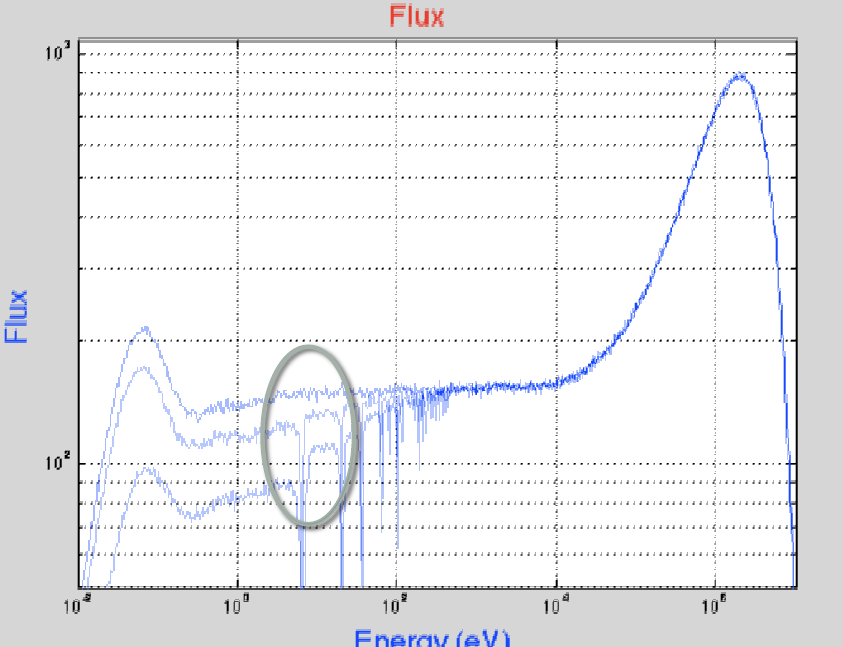
\includegraphics[width=3in]{images/r-m/resonance-1-over-E.png}
  \caption{The 1/E Spectrum Above A Resonance Suggests Group XS Independent of Higher Energy Absorption} \label{1overE}
\end{figure}



%%%%%%%%%%%%%%%%%%%%%%%%% RESONANCE ESCAPE PROBABILITY %%%%%%%%%%%%%%%%%%%%%%%%
\clearpage
\subtopic{Resonance Escape Probability}
We define $p$ as the ratio of the therm neutron absorption rate over absorption rate at all energies; it is the fraction of neutrons absorbed thermally over all neutrons absorbed in the cell; hence it is the probability that a neutron will escape capture at energies above thermal; finally since most of the non-thermal capture in natural or slightly enriched uranium lattices is in the resonance part of the slowing down region, it is the \hi{resonance escape probability}\footnote{Henry, p. 110}. 
\begin{align}
p &= \exp \left( - \frac{N_R \RI_{\eff}}{\xi \Sigma_m} \right)  = \exp \left( - \frac{\RI_{\eff}}{\xi \sigma_d} \right)
\end{align}
Notice: (1) this expression is only an approximation; (2) \textit{p only depends on effective RI and dilution cross section.} For instance, in a hydrogen system with $\sigma_d = 200$, we can tabulate the p values as in Table~\ref{p-values}. The last entry tells us that \textit{about 20\% of neutrons are absorbed in U238 resonances.}
\begin{table}
  \centering
  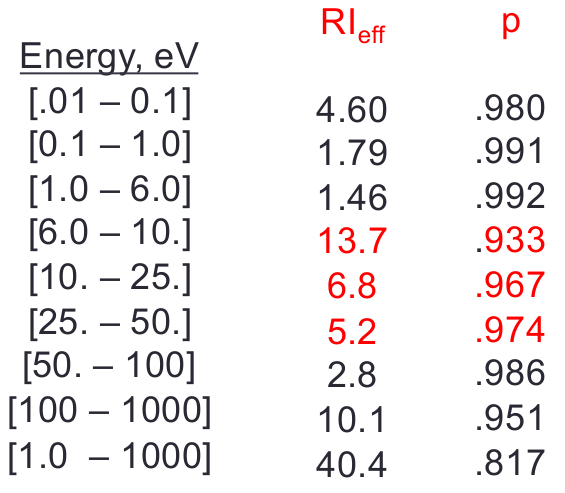
\includegraphics[width=1.5in]{images/r-m/resonance-escape-probability.png}
  \caption{Resonance Escape Probability For A Hydrogen System} \label{p-values}
\end{table}

\textbf{Derivation of $p$ expression:}
\begin{enumerate}
\item Assumptions: only elastic down scatter above the resonance, $\sigma_{a,m} = 0, \sigma_{s} = $const, and only a single resonance absorber. 
\item Start from our balance equation (scattering in = resonance absorption),
\begin{align}
\frac{S}{\zeta(u)} \du &= \left[ N_r \sigma_{a,r} (u) + \Sigma_m \right] \phi(u) \du = N_r \left[ \sigma_{a,r} (u) + \sigma_d \right] \phi(u) \du \\
\Rightarrow \phi(u) &= \frac{S}{\zeta(u) N_r \left[ \sigma_{a,r} (u) + \sigma_d \right] } 
\end{align}
Define resonance escape probability as:
\begin{align}
p &= \frac{S - \int N_r \sigma_a(u) \phi(u) \du}{S} \\
&= 1 - \frac{\int N_r \sigma_a(u) \frac{S}{\zeta(u) N_r \left[ \sigma_{a,r} (u) + \sigma_d \right] } \du }{S} \\
&= 1 - \int \frac{\sigma_{a,r} (u) }{\zeta(u) \left[ \sigma_{a,r} (u) + \sigma_d \right] } \du
\end{align}
\item Assume the mean logarithmic energy decrement is independent of lethargy, 
\eqn{ p = 1 - \frac{1}{\zeta} \int \frac{\sigma_{a,r} (u)}{\sigma_{a,r} (u) + \sigma_d} \du }
\item Use our definition of effective RI,
\eqn{ \RI_{\eff}^{u1 \to u2} = \int_{u1}^{u2} \frac{\sigma_{a,r} (u) \sigma_d}{\sigma_{a,r} (u) + \sigma_d} \du }
We can write $p$ in terms of $\RI$:
\eqn{ \boxed{p^{1\to 2} = 1 - \frac{\RI_{\eff}^{u1 \to u2}}{\zeta \sigma_d} } }
\item Since the source is incrementally reduce with each successive resonance,
\eqn{ p^{u1 \to uN} = \left( 1 - \frac{\RI_{\eff}^{u1 \to u2}}{\zeta \sigma_d} \right) \left( 1 - \frac{\RI_{\eff}^{u2 \to u3}}{\zeta \sigma_d} \right)
  \cdots \left( 1 - \frac{\RI_{\eff}^{uN-1 \to uN}}{\zeta \sigma_d} \right) }
We approximate the sequence as,
\eqn{ p^{u1 \to uN} = \exp \left( - \frac{\Sum_{u1}^{uN-1} \RI_{\eff}^u}{\zeta \sigma_d} \right) }
or
\eqn{ \boxed{ p \approx \exp \left( - \frac{\RI_{\eff}}{\zeta \sigma_d} \right) = \exp \left( - \frac{N_r \RI_{\eff}}{\zeta \Sigma_m} \right)  } }
which for hydrogen system becomes, 
\eqn{ p \approx \exp \left( - \frac{\RI_{\eff}}{\sigma_d} \right) }
\end{enumerate}






\end{document}

\documentclass{school-22.211-notes}
\date{February 27, 2012}

\begin{document}
\maketitle


\clearpage
%%%%%%%%%%%%%%%%%%%%%%%%% Resonance Models Day 3: Important properties %%%%%%%%%%%%%%%%%%%%%%%%%%%%
\topic{Important Properties}
\subtopic{Doppler Broadening/Temperature Effects On Cross Section}
Doppler effect describes the importance of thermal agigation on cross section. Thermal equilibrium means: 
\begin{itemize}
\item All heat source are perfectly balanced and the temperature of the medium is assumed constant. 
\item Atom energy/velocity distribution can be approximated by Maxwell-Boltzman distribution, that is, a probability distribution that expresses velocity distribution as a function of temperature and mass medium. The higher the temperature, the wider the velocity range is; the lighter the atom is, the wider the velocity range is. Know the Boltzmann constant. 
\end{itemize}

U238 has a negative Doppler feedback. Reason: as temperature increases, the resonance width increases with its depth decreases. We care less about the depth, because there is no neutrons present right at the peak anyway. 


\hi{Doppler Broadening} means, as the temperature increases, the width of the spectrum increases, although the area under the curve stays the same\footnote{References: Reuss Section 8.4; Handbook of Nuclear Engineering Chapter 4 Section 3; Duderstadt p.337-338; Bell p.433 (points out the area under the cross section curve is constant; hence the absorption rate is proportional to the magnitude of the flux in a sense.)}. 
There are two possibilities: 
\begin{enumerate}
\item Infinite RI (infinite dilution factor, negligible absorber concentration, $\Sigma_t \sim \Sigma_s^M$) is independent of temperature becase the area under the psi chi curves are constant. The absorber concentration is too low to perturb the flux, hence no flux depression and no self-shielding.  
\item Effective RI (finite concentration of \ce{^{238} U}) is dependent of temperature and the resonant material density because of the energy self-shielding effect as in Figure~\ref{Doppler}: 
  \begin{itemize}
  \item If temperature increases, $\RI_{\eff}$ would increase, because the broadened resonance increases the energy range over which abosrption occurs, which outweighs the lowering of the resonance peak. Reason: Energy self-shielding (the strong absorption of the resonance tends to shield the absorber nucleir from neutrons with energy $E\sim E_0$, hence the term `flux depression').  As temperature increases, the resonance is broadened by the Doppler effect, the neutron flux depression is decreased, whereas the area under the cross section curve is essentially constant. Hence the resonance absorption which is the energy-integrated reaction rate $\Sigma_a(E) \phi(E)$ increases with increasing temperature. 
  \item If U/H increases, there are two consequences: one is that the flux is more depressed hence the $\RIeff$ decreases; secondly the higher energies become more important as we would later see in Section~\ref{spectral-hardening-section}. 
  \item \textit{The higher the concentration of U238, the larger the Doppler temperature effects become.}
  \end{itemize}
\end{enumerate}


\textbf{Why do resonance broaden?} 

If a neutron's energy equals that of the resonance, it will be absorbed. If it is
slightly above or below the resonance energy, it will scatter off the U-238 nuclei
without absorption. As the fuel heats up, the nuclei vibrate and this changes the
relative speed between the neutron and the nuclei. Hence, the neutron is
effectively at a different energy. What are the consequences? Suppose a neutron
is initially slightly below the resonance energy. If the nucleus moves toward the
neutron, the relative speed between the two goes up. Hence, that neutron will be
absorbed.

But for every neutron that is now newly absorbed, one that was previously at the
resonance energy is now too high and it only scatters off the nucleus. So, why is
there a net increase in absorption? The reason is that scattered neutron loses only
a slight amount of energy (small object bouncing off a large one) and on its next
collision, which will likely be with the fuel again, it will be absorbed. Thus, U-
238 resonances broaden because (1) the U-238 nuclei vibrate more rapidly on heat
up and (2) the fuel is separate from the coolant so that successive interactions
occur in the fuel.

\begin{figure}
  \begin{subfigure}[b]{0.45\textwidth}
    \centering
    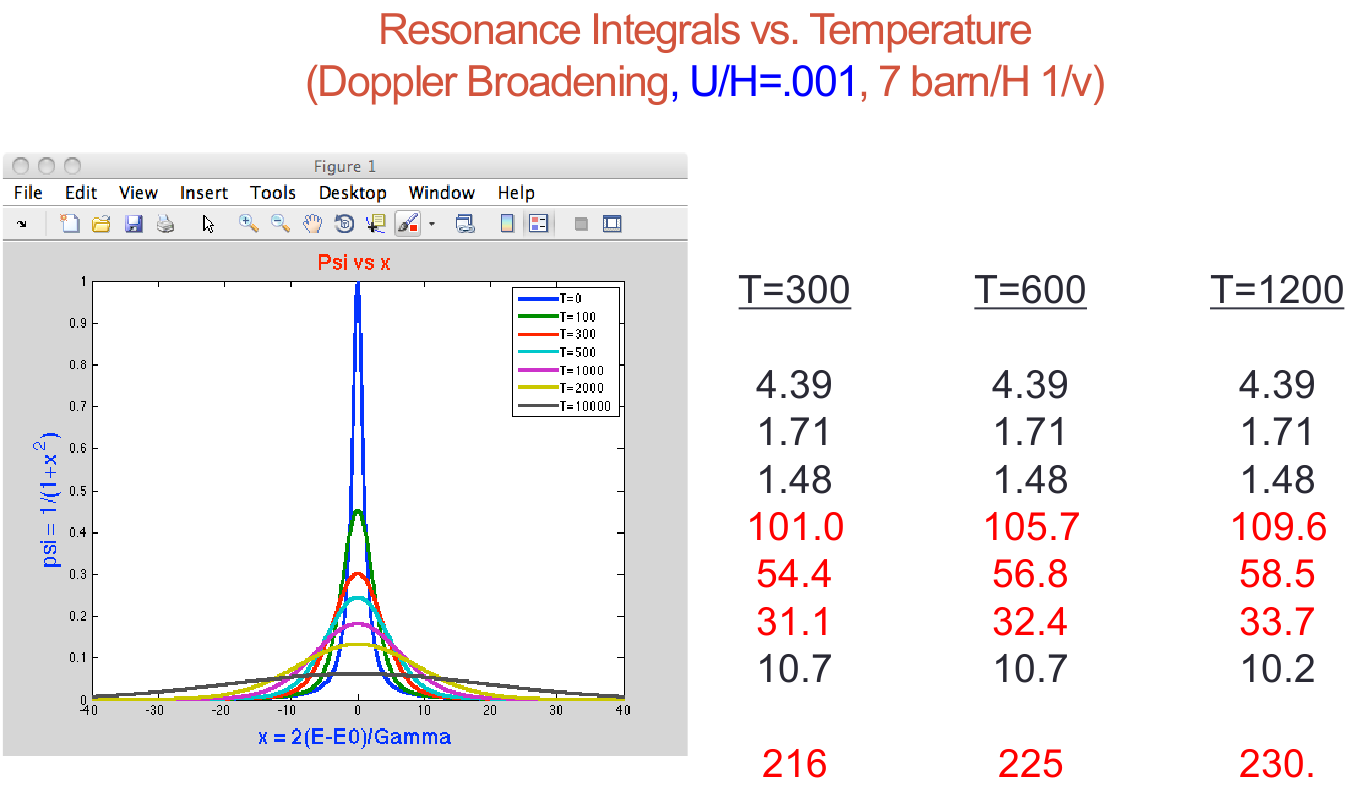
\includegraphics[width=\textwidth]{images/r-m/Doppler-RI-1.png}
    \caption{U/H = 0.001} \label{UH0.01}
  \end{subfigure}
  \begin{subfigure}[b]{0.45\textwidth}
    \centering
    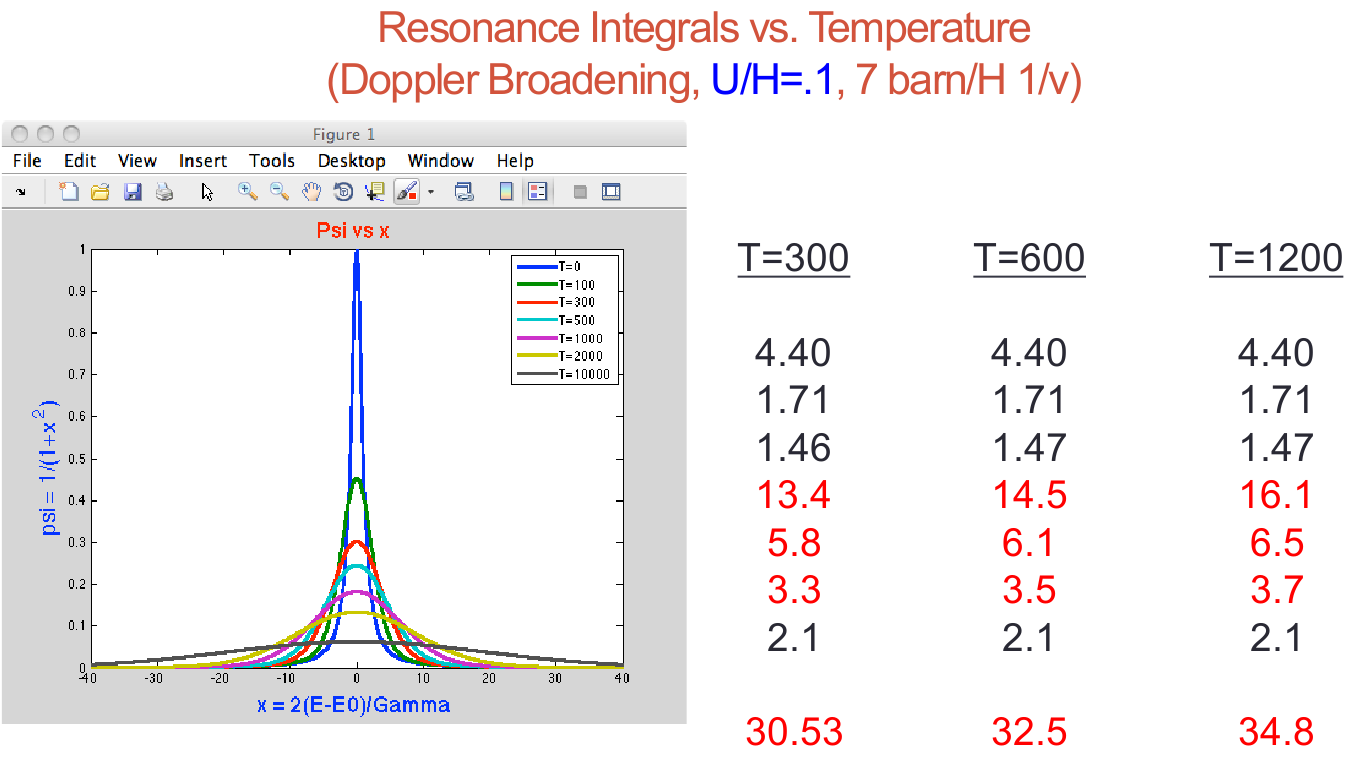
\includegraphics[width=\textwidth]{images/r-m/Doppler-RI-2.png}
    \caption{U/H = 0.1} \label{UH0.1}
  \end{subfigure}
  \caption{Impact of Temperature On Effective RI, Doppler Broadening} \label{Doppler}
\end{figure}


\clearpage
%%%%%%%%%%%%%%%%%%% SELF-SHIELDING %%%%%%%%%%%%%%%%%%%%%
\subtopic{Spatial Self-Shielding}
Self-shielding/flux depression is first observed through: 
\begin{table}[ht]
  \centering
  \begin{tabular}{|l|p{6cm}|p{6cm}|} \hline
    & Observation & Explaination \\ \hline
    Spatial 
    & if natural uranium was made into a lump surrounded by moderator, resonance absorption $\down \down$  
    & U238 in the center of a pin is `shielded' from neutrons in the moderator \\ \hline
    Energy
    & if U/H $\up$, absorption rate per atom (for neutrons slowed down in a water \& U mix) $\down$   
    & the magnitude of absorption is proportional to the width of the resonance;  \\ \hline
  \end{tabular}
  \caption{Observation Concerning Self-Shielding}
  \end{table}

In a sentence, lumped configuration shields the fuel region from neutrons with $E \sim E_0$, hence decreasing resonance absorption and increasing $p$. As fuel diameter increases, the RI -- and therefore the absorption -- decreases. 

For a homogenized medium, the value of p for natural uranium is about 0.70.
However, larger values exist for the heterogeneous case. This is because of a
phenomenon called ``spatial self-shielding.'' The idea is to keep the fuel and
moderator separate. Neutrons slow down in a stepwise manner. Some collisions
will cause neutrons to jump over the energies that correspond to the U238
resonances. Others will land in resonance energies. What happens to these neutrons? 
Suppose a neutron has an energy close to that of a U-238 resonance. 
\begin{itemize}
\item If a neutron scatters off U238 it will lose
only a small amount of energy. In this case, the neutron is
left near the resonance energy.
\item If it scatters off moderator it will lose a lot of its energy.  In this case the neutron is removed from that energy.
\end{itemize}

What then is the effect of homogeneous or heterogeneous fuel? If the fuel and
moderator are separate and the neutron is in the moderator, chances are it will
collide with another moderator atom and be scattered out of the resonance region.
So, heterogeneous arrangements favor resonance escape. In contrast, if the fuel
and moderator are infinitely mixed (homogeneous) or if the fuel rod/moderator
volumes repeat on small scales with dimensions less than a diffusion length, the
next collision may again be with fuel and the neutron will be absorbed.
Heterogeneous arrays are sometimes called ``lumped'' meaning that the fuel and
moderator are separate, widely spread entities.

Notice both $f$ and $p$ depends on the moderator-to-fuel ratio and there is a trade-off
between the two\footnote{It should be noted that if one separates the fuel and moderator (large amounts of
moderator between fuel rods), one decreases the thermal utilization. For f to be
large, one seeks to maximize absorption in the fuel and hence minimize spatial
self-shielding which could lead to absorption in the moderator. Thus, there is a
tradeoff between f and p. Both depend on the moderator-to-fuel volume ratio.
Optimal designs have both f and p at about 0.9.}. 

\subtopic{Energy Self-shielding}
In a sentence, \textit{the strong absorption of the resonance tends to shield the absorber nuclei from neutrons with energy$\sim E_0$, hence creating the flux depression at $E_0$.}

Forget: When pure scattering, we can assume the thermal flux to be Maxwellian. But as we increase absorption, the spectrum would harden. 

Example: compare spectrum of UOX and MOX. UOX is 4\% U235, 96\% U238. MOX is 8\% Pu (2/3 fissile, 1/3 parasitic absorber), 92\% U238. The reason MOX's thermal spectrum is depressed is, 
\begin{itemize}
\item 1/3 of Pu in MOX is parasitic absorbtion, thus decreasing the thermal spectrum. 
\item Pu239's fission cross section is significantly larger than U235's fission cross section, thus depressing the spectrum.
\item Pu has huge thermal resonances. 
\end{itemize}




Kord: 

As we increase the U/H ratio, the RI decreases in the three big resonance regions, and we see big dips on the spectrum plot. There are so much U238 in the fuel, that there is no flux in the fuel anymore. 

As we increase the number of uranium atoms by a factor of 10, the number of absorption per atom is decreased by a factor of 3. That is, the total aborption still increases, but the absorption per atom decreases. Figure~\ref{energy-self-shielding} illustrates that RI are very dependent on the density of resonant materials.
\begin{figure}
  \centering
  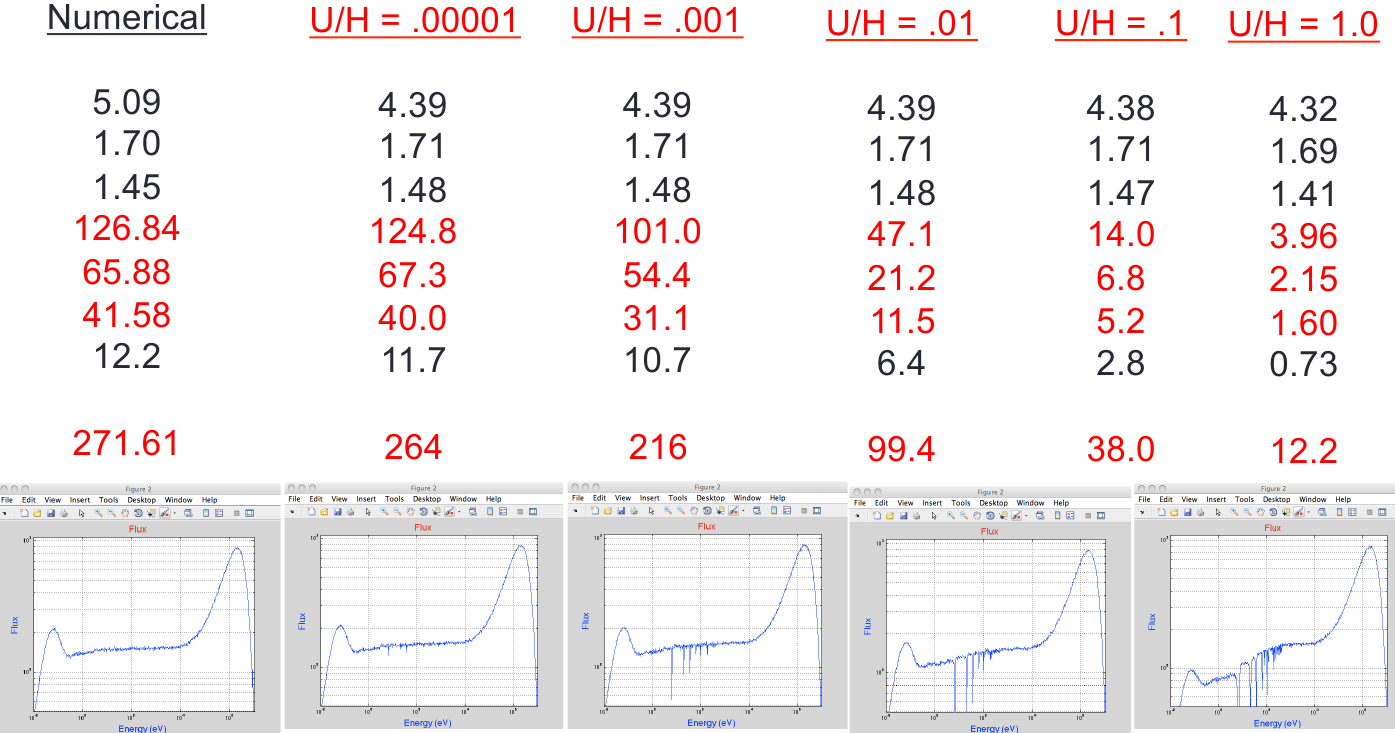
\includegraphics[width=4.5in]{images/r-m/self-shielding.png}
  \caption{Impact of Energy Self-Shielding On Effective RI} \label{energy-self-shielding}
\end{figure}



\clearpage
%%%%%%%%%%%%%%%%%%%%% SPECTRAL HARDENING %%%%%%%%%%%%%%%%%%
\subtopic{Spectral Hardening Shifts Resonant Absorption Rates}\label{spectral-hardening-section}
As U/H increases, the higher energy ranges become more important, and the peak of the thermal spectrum shifts to the right. Distribution of group-wise absorption shifts towards the higher energy. $1/v$ absorption of U238 becomes more significant. Self-shielding reduces the large resonance absorption fractions. See Figure~\ref{spectral-hardening}. 
\begin{figure}[ht]
  \centering
  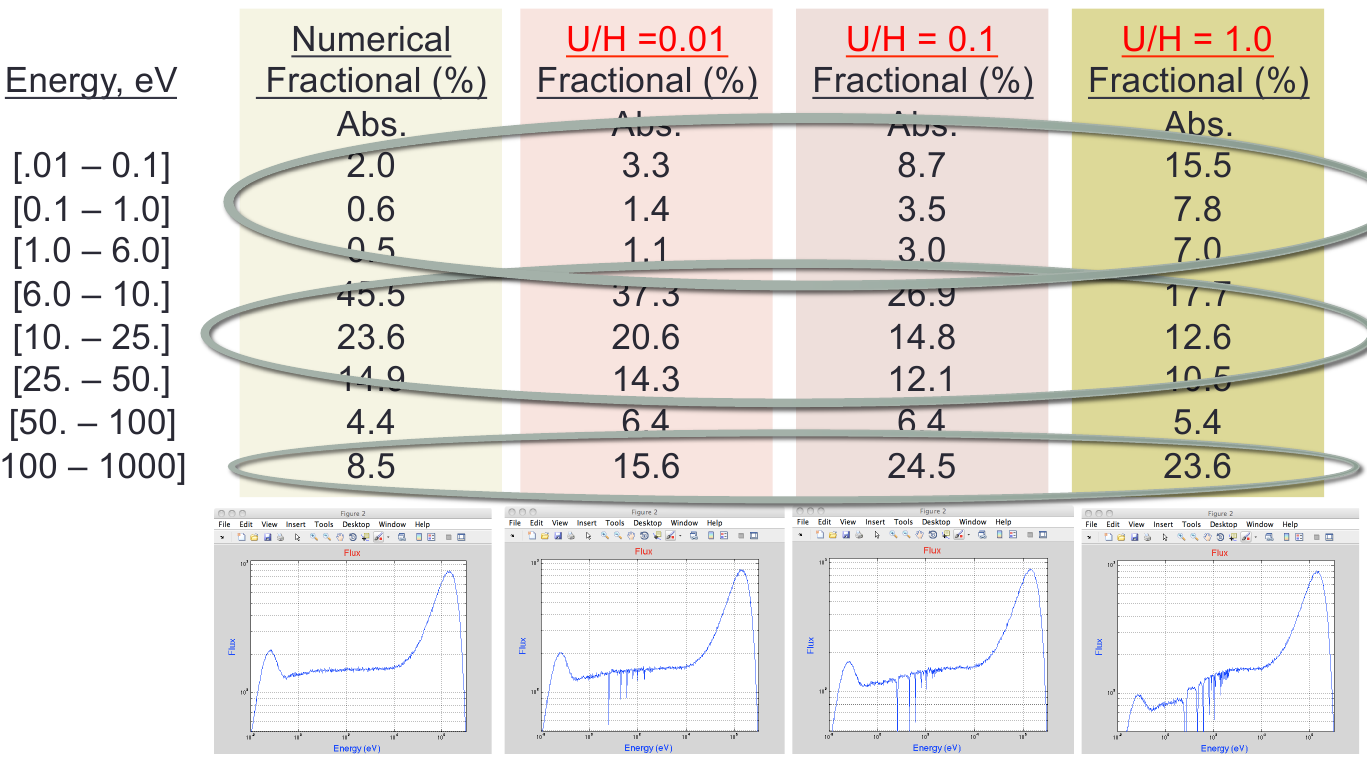
\includegraphics[width=6in]{images/r-m/spectral-hardening.png}
  \caption{Impact of Spectral Hardening On RI} \label{spectral-hardening}
\end{figure}

As Shultis states(p.286-297),

``As the temperature of the core material increases, the thermal neutrons maintain a Maxwellian energy distribution one but shifted increasingly towards higher energies. The thermal spectrum is said to harden. If all the cross sections in the core
had exactly a 1/v dependence, there would be no change in the thermal-neutron
interaction rates. However, most heavy nuclides have resonances near the upper end
of the thermal energy range and their cross sections, consequently, are not exactly
1/v in the thermal energy region. For example 239Pu has a large resonance at about 0.3 eV, and, as the thermal neutrons shift in energy towards this resonance, more neutrons are absorbed by 239Pu and thus the fission rate increases, thus producing a positive reactivity feedback. By contrast, hardening the thermal neutron spectrum causes a very slight decrease in absorption by 235U. 

This hardening of the thermal neutron spectrum with increasing temperature
is taken to an extreme in the TRIGA class of reactors which use as fuel enriched 235U blended in zirconium hydride. As the fuel temperature increases, vibrating hydrogen atoms trapped in the zirconium-hydride crystal lattice can transfer some
of their vibratiorial energy (about 0.13 eV) to thermal neutrons, thereby removing
them from the thermal energy region so they are less likely to be absorbed by the
fuel. This very rapid negative reactivity feedback effect is the reason these reactors
can be operated in a pulse mode, in which a large positive reactivity is inserted into
the core by rapidly removing a control rod to make the reactor very super prompt
critical. However, the ZrH negative temperature feedback acts within a few ms to
stop the runaway chain reaction, which has increased the reactor power by many
thousands of times the initial power, and brings the reactor power back to safe
limits.'' 


\subtopic{Impact On Design}
\eqn{ \kinf = \epsilon p \eta f}
$\epsilon$ is fast fission. 
\eqn{ \epsilon = \frac{\int_{F+T} \Sigma_f^F (E) \phi_F \dE}{\int_T \Sigma_f^F \phi_F \dE} }

$p$ is resonance escape probability, 
\eqn{ p = \frac{V_F \int_T \Sigma_a^F \phi_F \dE + V_M \int_T \Sigma_a^M \phi_M \dE}{V_F \int_{T+I} \Sigma_a^F \phi_F \dE + V_M \int_{T+I} \Sigma_a^M \phi_M \dE }  \approx \exp \left[ - \frac{V_F N_F \RI}{\Sum_i (V \xi \Sigma_s)_i} \right] }

$eta$ is 
\eqn{\eta = \frac{\int_T \nu \Sigma_f^F \phi_F \dE}{\int_T \Sigma_a^F \phi_F \dE}  }

$f$ is
\eqn{ f = \frac{V_F \int_T \Sigma_a^F  \phi_f \dE}{V_F \int_T \Sigma_a^F \phi_F \dE + V_M \int_T \Sigma_a^M \phi_M \dE} }


Insert image here. Maximum $k$ gives us the optimal design (in terms of moderation). In reality we always operate at slightly under moderated. With Boron in it, we need to operate at even under moderation, and have to limit Boron concentration to 2000 ppm. Because now if we lose water, we not only lose moderation, but also lose absorption, and when Boron concentration is to high, we lose more absorption than moderation, which actually create a positive coefficient. 


\end{document}

\documentclass{school-22.211-notes}
\date{February 29, 2012}

\begin{document}
\maketitle



%%%%%%%%%%%%%%%%%%%%%%%%% Resonance Models Day 4 %%%%%%%%%%%%%%%%%%%%%%%%%%%%
\clearpage
\topic{Dilution Cross Section/Dilution Factor}
In an infinite homogeneous medium with one resonance absorber and one moderator,  we write removal rates equals scattering rates (see Reuss 8.2.1 for a similar derivation), 
\begin{align}
\left[ N_r \sigma_r (u) + N_m \sigma_m (u) \right] \phi (u) &= \int_{-\infty}^u N_m \sigma_m (u') \phi(u') P(u' \to u) \du' \\ 
&= N_m \sigma_m \int_{-\infty}^u \phi(u') P(u' \to u) \du' \\
&= N_m \sigma_m C \\
\phi(u) &\propto \frac{N_m \sigma_m}{N_r \sigma_r(u) + N_m \sigma_m} \\
\phi(u) &\propto \frac{ \frac{N_m}{N_r} \sigma_m}{\sigma_r(u) + \frac{N_m}{N_r} \sigma_m}  \label{flux-shape}
\end{align}
In the above derivation we made two assumptions:
\begin{itemize}
\item The moderator's xs is independent of energy near resonances. For almost any moderators we can pick, the assumption that the elastic scattering xs is constant is valid in the thermal range as in Figure~\ref{scatter-xs}. 
\item $\int \phi(u') P(u' \to u) \du'$ is constant. We know that the flux above the resonance is 1/E and hence constant in lethargy. If we assume scattering into the resonance comes from this constant lethargy region, then the resonance lethargy is constant as well. 
\end{itemize}
Eq.~\ref{flux-shape} suggests that \textit{in infinite medium the flux shape near resonance depends only on the ratio of the number density of the moderator to the resonance absorber and the moderator cross section.} But once we move into a finite medium or we take into account leakage, then the absolute number densities are needed.
 
To capture the ratio of number densities and the moderator cross section, we define \hi{dilution cross section} as,
\eqn{ \boxed{ \sigma_d = \frac{N_m \sigma_m}{N_r} } }
Then the flux shape near resonance is,
\eqn{ \boxed{ \phi(u) \propto \frac{\sigma_d}{\sigma_r + \sigma_d} } }
This flux shapes let us to compute approximated effective RI. Recall RI is defined as, $\RI = \int \sigma_r (u) \du$. Then the approximated effective RI is,
\eqn{ \boxed{ \RI_{\eff} = \int \sigma_r(u) \frac{\sigma_d}{\sigma_r + \sigma_d} \du }  }
Two extremes of $\RI_{\eff}$ and $\sigma_d$:
\begin{itemize}
\item As $\sigma_d \to \infty$, the entire media is moderator, we reach the limit of infinite dilute, $\RI_{\eff} \to \RI$; we should get within 1\% of the ENDFVII xs data;
\item As $\sigma_d \to 0$, analytically our assumptions do not hold true any more, but the MC is true that as $\RI_{\eff} \to 0, \phi \to 0$ as seen in Figure~\ref{energy-self-shielding}. Interpretation: as we have no moderator, every atom is essentially self-shield because they are all resonant isotopes, hence infinite flux depression.  
\end{itemize}
The scattering down to resonance is independent of the resonance. In other words, if the spectrum above a resonance returns to 1/E as in Figure~\ref{1overE}, the group cross sections will be independent of higher energy absorptions. This may be related to what we talk about before, that 
\begin{figure}
  \centering
  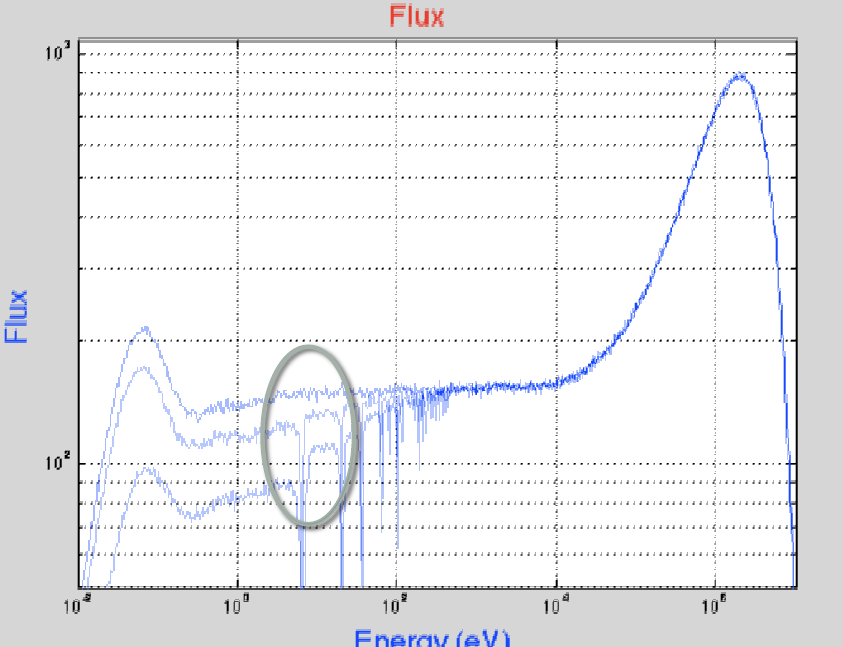
\includegraphics[width=3in]{images/r-m/resonance-1-over-E.png}
  \caption{The 1/E Spectrum Above A Resonance Suggests Group XS Independent of Higher Energy Absorption} \label{1overE}
\end{figure}


\clearpage
%%%%%%%%%%%%%%%%%%%%%%%%% RESONANCE ESCAPE PROBABILITY %%%%%%%%%%%%%%%%%%%%%%%%
\topic{Resonance Escape Probability}
We define $p$ as the ratio of the therm neutron absorption rate over absorption rate at all energies; it is the fraction of neutrons absorbed thermally over all neutrons absorbed in the cell; hence it is the probability that a neutron will escape capture at energies above thermal; finally since most of the non-thermal capture in natural or slightly enriched uranium lattices is in the resonance part of the slowing down region, it is the \hi{resonance escape probability}\footnote{Henry, p. 110}. 
\begin{align}
p &= \exp \left( - \frac{N_R \RI_{\eff}}{\xi \Sigma_m} \right)  = \exp \left( - \frac{\RI_{\eff}}{\xi \sigma_d} \right)
\end{align}
Notice: (1) this expression is only an approximation; (2) \textit{p only depends on effective RI and dilution cross section.} For instance, in a hydrogen system with $\sigma_d = 200$, we can tabulate the p values as in Table~\ref{p-values}. The last entry tells us that \textit{about 20\% of neutrons are absorbed in U238 resonances.}
\begin{table}
  \centering
  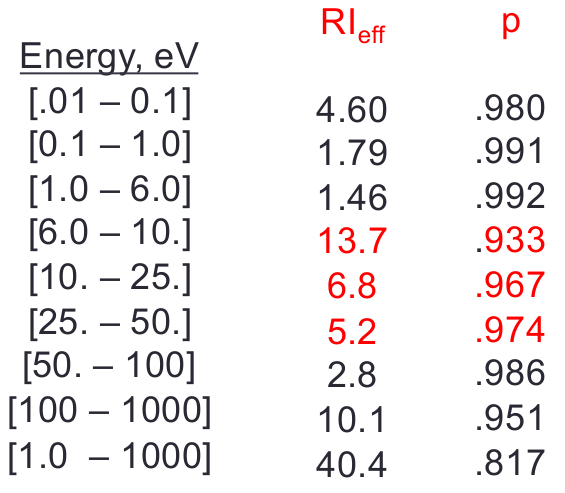
\includegraphics[width=1.5in]{images/r-m/resonance-escape-probability.png}
  \caption{Resonance Escape Probability For A Hydrogen System} \label{p-values}
\end{table}

\textbf{Derivation of $p$ expression:}
\begin{enumerate}
\item Assumptions: only elastic down scatter above the resonance, $\sigma_{a,m} = 0, \sigma_{s} = $const, and only a single resonance absorber. 
\item Start from our balance equation (scattering in = resonance absorption),
\begin{align}
\frac{S}{\zeta(u)} \du &= \left[ N_r \sigma_{a,r} (u) + \Sigma_m \right] \phi(u) \du = N_r \left[ \sigma_{a,r} (u) + \sigma_d \right] \phi(u) \du \\
\Rightarrow \phi(u) &= \frac{S}{\zeta(u) N_r \left[ \sigma_{a,r} (u) + \sigma_d \right] } 
\end{align}
Define resonance escape probability as:
\begin{align}
p &= \frac{S - \int N_r \sigma_a(u) \phi(u) \du}{S} \\
&= 1 - \frac{\int N_r \sigma_a(u) \frac{S}{\zeta(u) N_r \left[ \sigma_{a,r} (u) + \sigma_d \right] } \du }{S} \\
&= 1 - \int \frac{\sigma_{a,r} (u) }{\zeta(u) \left[ \sigma_{a,r} (u) + \sigma_d \right] } \du
\end{align}
\item Assume the mean logarithmic energy decrement is independent of lethargy, 
\eqn{ p = 1 - \frac{1}{\zeta} \int \frac{\sigma_{a,r} (u)}{\sigma_{a,r} (u) + \sigma_d} \du }
\item Use our definition of effective RI,
\eqn{ \RI_{\eff}^{u1 \to u2} = \int_{u1}^{u2} \frac{\sigma_{a,r} (u) \sigma_d}{\sigma_{a,r} (u) + \sigma_d} \du }
We can write $p$ in terms of $\RI$:
\eqn{ \boxed{p^{1\to 2} = 1 - \frac{\RI_{\eff}^{u1 \to u2}}{\zeta \sigma_d} } }
\item Since the source is incrementally reduce with each successive resonance,
\eqn{ p^{u1 \to uN} = \left( 1 - \frac{\RI_{\eff}^{u1 \to u2}}{\zeta \sigma_d} \right) \left( 1 - \frac{\RI_{\eff}^{u2 \to u3}}{\zeta \sigma_d} \right)
  \cdots \left( 1 - \frac{\RI_{\eff}^{uN-1 \to uN}}{\zeta \sigma_d} \right) }
We approximate the sequence as,
\eqn{ p^{u1 \to uN} = \exp \left( - \frac{\Sum_{u1}^{uN-1} \RI_{\eff}^u}{\zeta \sigma_d} \right) }
or
\eqn{ \boxed{ p \approx \exp \left( - \frac{\RI_{\eff}}{\zeta \sigma_d} \right) = \exp \left( - \frac{N_r \RI_{\eff}}{\zeta \Sigma_m} \right)  } }
which for hydrogen system becomes, 
\eqn{ p \approx \exp \left( - \frac{\RI_{\eff}}{\sigma_d} \right) }
\end{enumerate}




\end{document}

\documentclass{school-22.211-notes}
\date{March  5, 2012}

\begin{document}
\maketitle

\clearpage
\topic{Heterogeneous Geometry Resonant Approximations} \label{heterogeneous-geo}
This is probably the most important topic in generating cross section in reactor physics. We want to take into account both the spatial and energy structure distributions of flux within each resonance when solving the neutron slowing down problem. 

\begin{enumerate}
\item Assumptions for heterogeneous geometry resonant approximations:
\begin{itemize}
\item All neutron interactions in moderator are purely scattering;
\item Moderator scattering xs is independent of energy;
\item The previous two points together leads to that the slowing down energy source in fuel and moderator is 1/E;
\item Slowing down source is spatially uniform within each region (a fairly accurate assumption);
\item A single resonance absorber species exists only in the fuel;
\item Fuel scattering removes neutrons from resonance energy (that is, narrow resonance model); 
\end{itemize}

\item Spatial Reciprocity Theorem. First we introduce the reciprocity condition. The only assumption we make for this theorem is that the source is flat. This theorem does not depend on geometry. 

Given two homogeneous region 1 and 2, the probability of going from point A in 1 to point B in 2 without colliding is:
\eqn{ \frac{e^{-\tau}}{4 \pi R^2} }
where $\tau = \frac{x_1}{\lambda_1} + \frac{x_2}{\lambda_2} = x_1 \Sigma_1 + x_2 \Sigma_2$. The probability of going from A to B and then colliding at B is: 
\eqn{ \frac{e^{-\tau}}{4 \pi R^2} \Sigma_2 }
The probability of going from A to any point in region 2 and colliding is:
\eqn{ \int \frac{e^{-\tau}}{4 \pi R^2} \Sigma_2  \dV_2}
The probability of a uniform spatial neutron source in region 1 going to any point in region 2 and colliding is:
\eqn{ \int \dV_1 \int \frac{e^{-\tau}}{4 \pi R^2} \Sigma_2  \dV_2}
The average probability per unit volume of a uniform source neutron going from region 1 to 2 and colliding is:
\eqn{ P_{1\to 2} = \frac{\Sigma_2}{V_1} \int \dV_1 \int \frac{e^{-\tau}}{4 \pi R^2}  \dV_2}
Likewise,
\eqn{ P_{2\to 1} = \frac{\Sigma_1}{V_2} \int \dV_2 \int \frac{e^{-\tau}}{4 \pi R^2}  \dV_1}
Since the two integrals are symmetric (that is, $P_{A\to B}$ and $P_{B \to A}$ are essentially the same), we can write,
\eqn{ P_{1\to 2} \frac{V_1}{\Sigma_2} = P_{2\to 1} \frac{V_2}{\Sigma_1} }
Hence we reach the reciprocity condition:
\eqn{ \boxed{ P_{1\to 2} \Sigma_1 V_1 = P_{2\to 1} \Sigma_2 V_2 } }

\item Two Region Balance Equations. 
First collision reaction rate balance, where $\sigma_{t,f}(u) = \sigma_{r,f} + \sigma_{pot, f}$ (the resonance absorption xs plus the potential scattering xs):
\eqn{ \overbrace{N_f \sigma_{t,f} (u) \Phi(u) V_f}^{\mbox{fuel region lost neutrons}} = \overbrace{Q_f V_f P_{f\to f} + Q_m V_m P_{m\to f}}^{\mbox{fuel region gain neutrons from slowing down sources}}  }
Because slowing down sources in both fuel and moderator are assumed to arise from the 1/E flux above the resonance energy, we can write
\eqn{ Q_m &= N_m \sigma_{s,m} \Psi(u) &  Q_f&= N_f \sigma_{pot, f} \Psi(u) }
Plug the slowing down sources back into the reaction rate balance equation, and recall $\Phi(u) = \Psi(u) \phi(u)$ where $\phi(u)$ is the \hi{fine structure energy shape of the flux for homogeneous mixture}, we extand the definition to define $\phi_f(u)$ as the heterogeneous energy shape of flux in fuel,
\eqn{ N_f \sigma_{t,f} (u) \phi_f (u) V_f = N_f \sigma_{pot, f} V_f P_{f\to f} + N_m \sigma{s,m} V_m P_{m\to f} }
Next we use reciprocity relationship,
\eqn{ P_{m\to f} N_m \sigma_m V_m = P_{f\to m} N_f \sigma_f V_f}
and substitute into the balance equation to get,
\eqn{ N_f \sigma_{t}^F (u) \phi_f (u) V_f = N_f \sigma_{pot}^F V_f P_{f\to f} + N_f \sigma_{t}^F V_f P_{f\to m} }
Then we replace $P_{f\to m} = 1 - P_{f\to f}$ and get, 
\eqn{ N_f \sigma_{t}^F (u) \phi_f (u) V_f = N_f \sigma_{pot}^F V_f P_{f\to f} + N_f \sigma_{t}^F V_f (1 - P_{f\to f}) }
Divide both sides by the number of neutrons, we get a balance equation in unit of cross section:
\eqn{ \sigma_{t}^F (u) \phi_f (u) = \sigma_{pot}^F P_{f\to f} +  \sigma_{t}^F (1 - P_{f\to f}) }
That is, if we know $P_{f\to f}$, we can solve for the spatially averaged energy shape of the flux in the fuel. 
\end{enumerate}

\clearpage
\subtopic{Wigner's Approximation of $P_{f\to f}$}
 Obtaining $\phi_f(u)$.
In this section we compute numerically the fuel-to-fuel first flight collision probability $P_{f\to f}$, hence obtaining an expression for the heterogeneous energy shape of flux in fuel $\phi_f(u)$. 

Wigner approximates $P_{f\to f}$ in terms of the mean chord length $l$: 
\eqn{ P_{f\to f} &\approx \frac{l N_f \sigma_{t,f} (u)}{1 + l N_f \sigma_{t,f} (u)} = \frac{\sigma_{t,f}(u)}{\frac{1}{l N_f} + \sigma_{t,f} (u)} }
Recall Cauchy's Theorem for any convex body, 
\eqn{ l = \frac{4V}{S} }
and define \hi{escape cross section},
\eqn{ \Sigma_e &= \frac{1}{l} & \sigma_e &= \frac{\Sigma_e}{N_f} }
$P_{f\to f}$ simplifies to, 
\eqn{ P_{f\to f} = \frac{\sigma_{t,f} (u)}{\sigma_{t,f} (u) + \sigma_e} }
Hence $\phi_f(u)$ can be written as, 
\eqn{ \boxed{ \phi_f (u) = \frac{\sigma_{pot, f} + \sigma_e}{\sigma_{t,f} (u) + \sigma_e } = \frac{\sigma_{pot, f} + \sigma_e}{\sigma_{r,f} (u) + \sigma_{pot, f} + \sigma_e} } }
\hi{Heterogeneous/Homogeneous Equivalence} suggests that the effects of heterogeneity are equivalent to some dilution cross section in a homogeneous mixture:
\begin{align}
\mbox{Homogeneous mixture energy shape of flux } \phi(u) &= \frac{\sigma_{pot, f} + \sigma_d}{\sigma_{r,f} (u) + \sigma_{pot, f} + \sigma_d}   & \sigma_d &= \frac{N_m \sigma_m}{N_r}  \\
\mbox{Heterogeneous energy shape of flux in the fuel } \phi_f(u) &= \frac{\sigma_{pot, f} + \sigma_e}{\sigma_{r,f} (u) + \sigma_{pot, f} + \sigma_e}   & \sigma_e &= \frac{S_f}{4 V_f N_r} 
\end{align}

\textbf{Example: calculate corresponding cross sections.} Given a PWR with a 0.41 cm radius pellet, \ce{^{238}U} number density of $4.0 \times 10^{22} \cm^{-3}$, enriched to 3\%, and fuel density is 10 g/cc. 
\begin{itemize}
\item If the system is homogeneous uranium and hydrogen, then the dilution cross section looks like:
\eqn{ \sigma_d &=  \frac{N_m \sigma_m}{N_r}  = \frac{1}{0.2} 20 \fsp \barn = 100 \fsp \barn/\mbox{resonance atom} }
If the system is 2 region, and we homogeneous the fuel region, then
\begin{align}
\sigma_e &= \frac{S_f}{4 V_f N_r} = \frac{2 \pi r h}{4 \pi r^2 h N_r} = \frac{1}{2 r N_r} = \frac{1}{(2)(0.41 \cm)(2.2 \times 10^{22} \cm^{-3})} \frac{1 \barn}{10^{-24} \cm^2} = 55 \fsp \barn/\mbox{resonance atom} \\
\sigma_b^{hom} &=  0.05 \sigma_{pot}^{235} + 2 \sigma_{pot}^O = 0.05 (11.3) + 2 (4.0) = 9 \fsp \barn \\
\sigma_b^{het} &= \sigma_b^{hom} + \sigma_e = 64 \fsp \barn \\ 
\sigma_s^F &= \sigma_{pot}^R + \sigma_b^{hom} = \sigma_{pot}^{238} + 0.05 \sigma_{pot}^{235} + 2 \sigma_{pot}^O = 11.4 + 0.05 (11.3) + 2 (4.0) = 20 \fsp \barn 
\end{align} 
\end{itemize}

\clearpage
\subtopic{Bell's Refinements of the Wigner's Collision Probability}. 
Bell Factor $b$ can be read off a plot given opacity (average chord times total cross section) and geometry (eg: homogeneous medium, infinite plate, sphere etc). It is then used to approximate $P_{f\to f}$ and hence $\phi_f(u)$:
\eqn{ P_{f\to f} &= \frac{\sigma_{t,f} (u)}{b \sigma_e + \sigma_{t,f} (u)}  & \phi_f(u) &=\phi_f (u) = \frac{\sigma_{pot, f} + b \sigma_e}{\sigma_{t,f} (u) + b \sigma_e }  }
Bell's refinement does nothing to the infinite opacity case, but could be a factor of 50\% or even a factor of 3 difference as opacity approaches zero. 
\begin{figure}[ht]
  \centering
  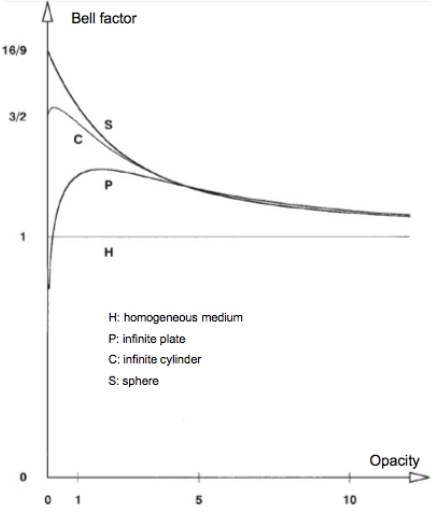
\includegraphics[width=3.5in]{images/r-m/bell.png}
  \caption{Bell's Factor for Various Geometris} \label{bell}
\end{figure}

\clearpage
\subtopic{Arrays of Rods, Dancoff Factor}
Notice our model so far is an isolated pin (that is, a fuel pin surrounded by an almost infinite moderator). Now we are going to discuss arrays of rods. The major difference is that not all neutrons leaving a fuel pin would have their next interaction in the moderator. 

We hence define the \hi{Dancoff Factor C}:
\eqn{ C = 1 - \frac{ \left. P_{f\to f} \right|_{\mbox{isolated rods}}}{ \left. P_{f\to f} \right|_{\mbox{arrays of rods}}}   }
$C$ depends on: the radius of the rods (in units of mean free path) and the lattice size/radius of rods, as plotted in Fig.~\ref{dancoff}. 
\begin{figure}[ht]
  \centering
  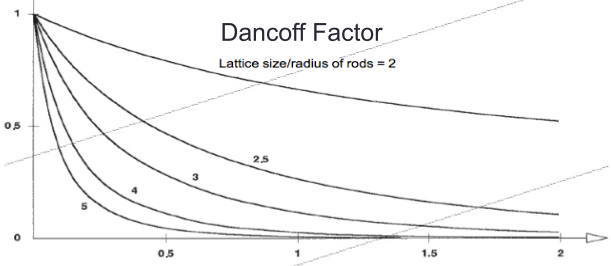
\includegraphics[width=4in]{images/r-m/dancoff.png}
  \caption{Dancoff Factor} \label{dancoff}
\end{figure}
\textbf{Notice if the moderator is opaque, the Dancoff factor becomes zero; if transparent, the Danoff factor trends to 1.0.}  LWRs typically have a C of 0.3. 
\eqn{ P_{f\to f}  = \frac{\sigma_{t,f} (u)}{\frac{(1-C)b}{(1-C) + Cb} \sigma_e + \sigma_{t,f} (u)}  } 
C changes the coefficient in front of the escape cross section from $\sigma_e \to \frac{(1-C)b}{1-C + Cb} \sigma_e$. For a typical PWR pin, that is reduced by 0.7 to 0.8.

\textbf{Example: Find Dancoff Factor.} Given water at 1 g/cc with a number density of $6.6 \times 10^{24}$ H atoms/cc, hydrogen xs of 20 barns, a PWR pin with 0.41 cm radius, a lattice pitch of 1.26cm. 
\begin{itemize}
\item We first find the mean free path: 
\eqn{ mfp = \frac{1}{\Sigma} = \frac{1}{N \sigma} =  \frac{1}{0.066 \times 10^{24} \times  20 \times 10^{-24}} =  0.76 \cm }
Then we find the parameter one, pellet radius over mfp = $\frac{0.41 \cm}{0.76 \cm}  = 0.54$, the other parameter is the lattice size over pellet radius $\frac{1.26 \cm}{0.41 \cm} = 3.07$. Using these two parameters, we can read off the plot that $C = 0.3$. For a Bell factor of about 1.1, the escape xs is reduced by,
\eqn{ \frac{ (1-C)b}{(1-C) + Cb} = 0.774} 
\end{itemize}


\clearpage
\subtopic{Carlvik's Refinements of the Bell's Collision Probability}
\eqn{ P_{ff} \approx \frac{\beta \sigma_{t,f}}{\alpha_1 + \sigma_e + \sigma_{t,f}} + \frac{(1-\beta) \sigma_{t,f}}{\alpha_2 \sigma_e + \sigma_{t,f}} }
where
\eqn{ \alpha_1 &= \frac{5A+6 - \sqrt{A^2 + 36A + 36}}{2(A+1)}, &\alpha_2 &= \frac{5A+6 + \sqrt{A^2 + 36A + 36}}{2(A+1)} &\beta&= \frac{\frac{4A+6}{A+1} - \alpha_1}{\alpha_2 - \alpha1} &A&= \frac{1-C}{C} }
Carlvik's two-term approximation is what is actually used in production tools nowaday. To use it, we essentially look up the resonance integral (or group xs) twice, once with $\sigma_e$ multiplied by $\alpha_1$ and the second time with $\sigma_e$ multiplied by $\alpha_2$, each of them are simple functions of the Dancoff factor: 
\eqn{ \RIeff = \beta \int_{u1}^{u2} \sigma_r (u) \frac{\sigma_{pot, f} + \alpha_1 \sigma_e}{\sigma_{r,f}(u) + \sigma_{pot, f} + \alpha_1 \sigma_e} \du + (1-\beta) \int_{u1}^{u2} \sigma_r (u) \frac{\sigma_{pot,f} + \alpha_2 \sigma_e}{\sigma_{r,f}(u) + \sigma_{pot,f} + \alpha_2 \sigma_e} \du }
To double check, 
\begin{itemize}
\item $C\to 1, \alpha_1 \to 0, \beta \to 1$, e.g., there is no escape from fuel.
\item $C\to 0, \alpha_1 \to 2, \alpha_2 \to 3, \beta \to 2$, e.g., isolated rod.
\item FOr intermediate values of $C$, each coefficient is a monotonic function.
\end{itemize}


\end{document}

\documentclass{school-22.211-notes}
\date{March  7, 2012}

\begin{document}
\maketitle

\topic{k-infinity In Infinite Medium Calculations (No Leakage)}


\eqn{ k_{\inf} =  \frac{\mbox{total fissions} \cdot \bar{\nu} }{\mbox{total absorptions}} = \frac{\int \dV \int \nu \Sigma_f \Phi \dE}{\int \dV \int \Sigma_a \Phi \dE} = \epsilon \eta f p }


Reference: Henry p. 104. 

\topic{Solving Two-Region Monte Carlo Spectral Analysis}
Review codes in Lec8. Review slide 22 on approximation of collision probabilities. 

\topic{Observations From Two-Region Monte Carlo Spectral Analysis}
\begin{enumerate}
\item With no oxygen or zirconium: flux dips in moderator are mild because there is only elastic scattering. 
\item Adding in Zr: Zr has massive elastic scattering resonances, hence creating fluctuations in both spectrums most noticable in energies right above the resonance energies. THe reactivity change is small (positive 560 pcm).
\item Adding in O: the fast flux looks distorded in both fuel and moderator, this is because the oxygen xs has werid dips in high energy xs. the reactivity change is not large (negative 680 pcm). 
\item Removing hydrogen absorption: the spectrum shape does not change much, but the reactivity change is huge (8808 pcm), because there are so much hydrogen in the system (hydrogen xs is 1/v down to 100 keV); this is why LWR fuel has to be enriched. 
\item Remove U238 fission: reduce reactivity by 2\% (negative -1910 pcm). Spectrum shape does not change. 
\end{enumerate}
Looking at the flux in the moderator divided by the flux in the fuel, we see that:
\begin{itemize}
\item Above resonance energies: fuel flux is depressed because absorption is high compared with fission; 
\item In resonance energies: larger than 1 because of fuel spectrums dips for the resonances; especially at the interval containing 6.7 eV;
\item Below resonance energies: the ratio is around 1, till we hit the really low energy (less than 0.1 eV), that there is a 1/E tail that the fuel flux gets depressed. 
\end{itemize}

\topic{HW4: Heterogeneous Spectral Calculations}
We are going to get all of our cross section data from pointwise ENDF cross section. 

Build table: use 0.01 log(E) spacing (that's about 25,000 bins) to re-generate tables from the reading-in cross section. 


\lecture{Exam 1 Review}
Know how to interprete thermal scattering pdf and cdf. Questions would be based on understanding of the physics. 

\textbf{Part 1: Background Info (see Ch 1-3 from Reuss)}
\begin{enumerate}
\item Number Density
\item Flux
\item Lethargy
\item Mean free path
\item 1/v absorption cross section: 
  \begin{itemize}
  \item Wave-particle duality suggests that slow neutrons see a larger portion of space than fast neutrons, which means that slow neutrons often have larger cross sections, which leads to the 1/v rule for absorption (Reuss, 2.4.1). 
  \item Reason: Breit-Wigner states that absorption cross section is ($i = \gamma$ for radiative capture and $f$ for fission etc):
    \eqn{ \sigma_i = \pi \bar{\lambda}^2 g \frac{\Gamma_n \Gamma_i}{(E - E_0)^2 + \Gamma^2/4}  }
    \begin{itemize}
    \item $\Gamma_f, \Gamma_{\gamma}, \Gamma_{\alpha}$ etc are independent to energy E; $\Gamma_n \sim \sqrt{E}$ (for s-wave);
    \item $\bar{\lambda}^2 \sim \frac{1}{E}$;
    \item The denominator is approximately equal to the constant $E_0^2$ assuming that $E, \Gamma$ are small compared to $E_0$.
    \end{itemize}
    Thus $\sigma_f, \sigma_c \sim \frac{1}{\sqrt{E}} \sim \frac{1}{v}$. Even if several resonances make a contribution, the reasoning remains valid. This reasoning is not valid if $E_0$ is close to zero. 
  \item Henry (p. 202) has a derivation for why $\sigma_a(E_r) \approx \frac{1}{v_r}$, but it is using Breit-Wigner for resonance xs. 
  \end{itemize}
\item 1/E spectrum: true except when resonant absorber is present (recall we keep using 1/E for spectrum above the resonance). It is characteristic of the scalar flux in the slowing down energy range, as long as there is no up-scattering and no fission source. It arises basically from the kinematics of the scattering interaction. However it gets distorted by the energy behavior of the scattering cross sections and by neutron-absorption processes (Henry, p. 90). Asymptotic elastic scattering for high energy would yield a 1/E spectrum. 
\item Maxwellian shapes.
\end{enumerate}


\textbf{Part 2: Physical components of Monte Carlo code}
\begin{enumerate}
\item Elastic scattering:
  \begin{itemize}
  \item Asymptotic elastic scattering for high energy (above 4eV): assume isotropic scattering in COM. Generate 1/E spectrum; asymptotic flux value is $\Phi_{as} (u) = \frac{S}{\xi \Sigma_s (u)}$ according to Reuss (7.2.3). 
  \item Thermal elastic scattering (below 4eV): use elastic scattering for monatomic (Maxwellian) free gas; may up-scatter;
  \end{itemize}
\item Simple bound thermal scattering: 
\eqn{ \sigma_{\mbox{bound}} = \left( 1 + \frac{1}{A_{\mathrm{atom}}} \right) \sigma_{\mathrm{free}} }
\item SLBW resonance models
\item Doppler broadening
\item Monte Carlo tallies
\item Resonance integrals: represents the average absorption xs characterizing the resonance, averaged over the flux within the resonance. It is sort of like the averaged reaction rate, or collision density. Definition:
\eqn{ \RIeff = - \int_{u1}^{u2} \sigma(u) \du = \int_{E_1}^{E_2} \sigma(E) \frac{1}{E} \dE }
Relating to $\sigma_g, \sigma_d$: 
\eqn{ \RIeff &= \sigma_g \ln{\frac{E_2}{E_1}}  & \RIeff^{u1\to u2} &= \int_{u1}^{u2} \sigma_a^R (u) \frac{\sigma_d}{\sigma_a^R(u) + \sigma_d} \du  }
\item Group cross sections $\sigma_g$: the contribution of the resonance to a flux-weighted multigroup cross section.
  \eqn{ \sigma_g = \frac{\RI_{\eff}}{\ln(E_2/E_1)} }
\item Background (dilution) cross section $\sigma_d$:
\item Narrow vs. wide resonance models
\item Resonance escape probability $p$: only depends on effective RI and dilution xs: 
\eqn{ \boxed{ p \approx \exp \left( - \frac{\RI_{\eff}}{\zeta \sigma_d} \right) = \exp \left( - \frac{N_r \RI_{\eff}}{\zeta \Sigma_m} \right)  } }
\item Homogeneous/heterogeneous equivalence: 
\begin{align*}
\mbox{Homogeneous mixture energy shape of flux } \phi(u) &= \frac{\sigma_{pot, f} + \sigma_d}{\sigma_{r,f} (u) + \sigma_{pot, f} + \sigma_d}   & \sigma_d &= \frac{N_m \sigma_m}{N_r}  \\
\mbox{Heterogeneous energy shape of flux in the fuel } \phi_f(u) &= \frac{\sigma_{pot, f} + \sigma_e}{\sigma_{r,f} (u) + \sigma_{pot, f} + \sigma_e}   & \sigma_e &= \frac{S_f}{4 V_f N_r} 
\end{align*}
\item Effective cross section $\sigma_e$: 
\eqn{ \sigma_e = \frac{1}{l N_f} = \frac{S}{4V N_f} }
\item 2-region reciprocity relation:
\eqn{ P_{1\to 2} \Sigma_1 V_1 = P_{2\to 1} \Sigma_2 V_2 }
\item Dancoff factors.
\end{enumerate}

\textbf{Part 3: Other important concepts}
\begin{enumerate}
\item Self-shielding:
\item Doppler effect:
\item Maxwellian distribution: 
  \begin{itemize}
  \item Fission emission spectrum: peak occurs at 1.7 MeV, average occurs at 2 MeV.
  \item Thermal flux spectrum: for an infintie source-free medium with small absorption cross section (as long as $\Sigma_a(E)$ is small compare to $\Sigma_s(E)$), the thermal spectrum is Maxwellian. The higher energy portion of the thermal region is approximately 1/E with slowing down source and absorption present (Henry, p.98). 
  \end{itemize}
\item Slowing down equations. 
\item Review of spectrum:
    \begin{enumerate}
      \item a high energy hump. Reason: fission spectrum, degraded due to scattering; 
      \item slight decrease in the epithermal region. Reason: resonant capture losses, esp. U238; 
      \item  a low energy hump. Reason: Maxwell distribution of the thermal agitation but a little harder because the temperature equilibrium has not been perfectly achieved. 
    \end{enumerate}
\end{enumerate}


%%%%%%%%%%%%%%%%%%%%%%%%% Qualify Exam Start %%%%%%%%%%%%%%%%%%%%%%%%%%%%
\lecture{Facts For Qualify Exam}
\begin{enumerate}
\item Common units, see Table~\ref{units}.
\begin{table}
  \centering
  \begin{tabular}{|c|c|c|c|} \hline
   $\sigma$ & $\Sigma$ & $\phi = nv$ & $R = \phi \Sigma$  \\ \hline
   $\cm^2$ & $1/\cm$ & $\frac{n}{\cm^2 \s}$ & $\frac{\mathrm{reactions}}{\cm^3 \s}$ \\ \hline
  \end{tabular}
  \caption{Units of Common Terms} \label{units}
\end{table}

\item Fast flux in hydrogen is around $10^{14}$ n/cm$^2$s, and on the order of $10^{12}$n/cm$^2$s for thermal flux. 

\item U235 fission xs at 0.1 eV is about 200 barns; Pu239 fission xs is about 500 barns. In thermal reactors, Pu absorption should be about twice that of uranium. 

\item Elastic Scatterin cross section as in Figure~\ref{scatter-xs}
\begin{figure}
  \centering
  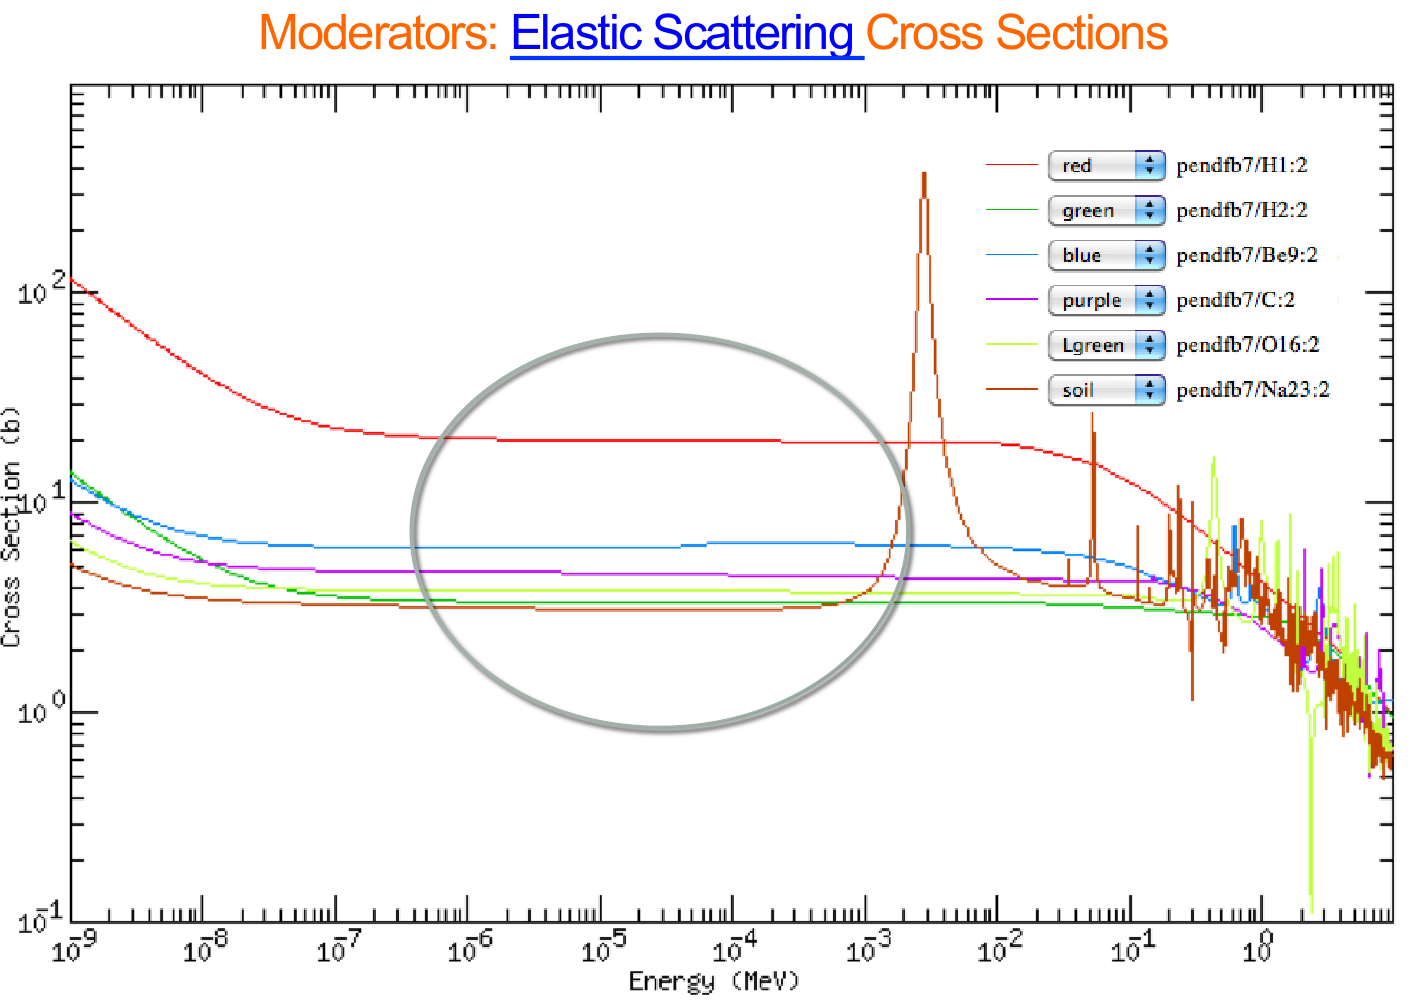
\includegraphics[width=4in]{images/scatter-xs-moderator.png}
  \\
  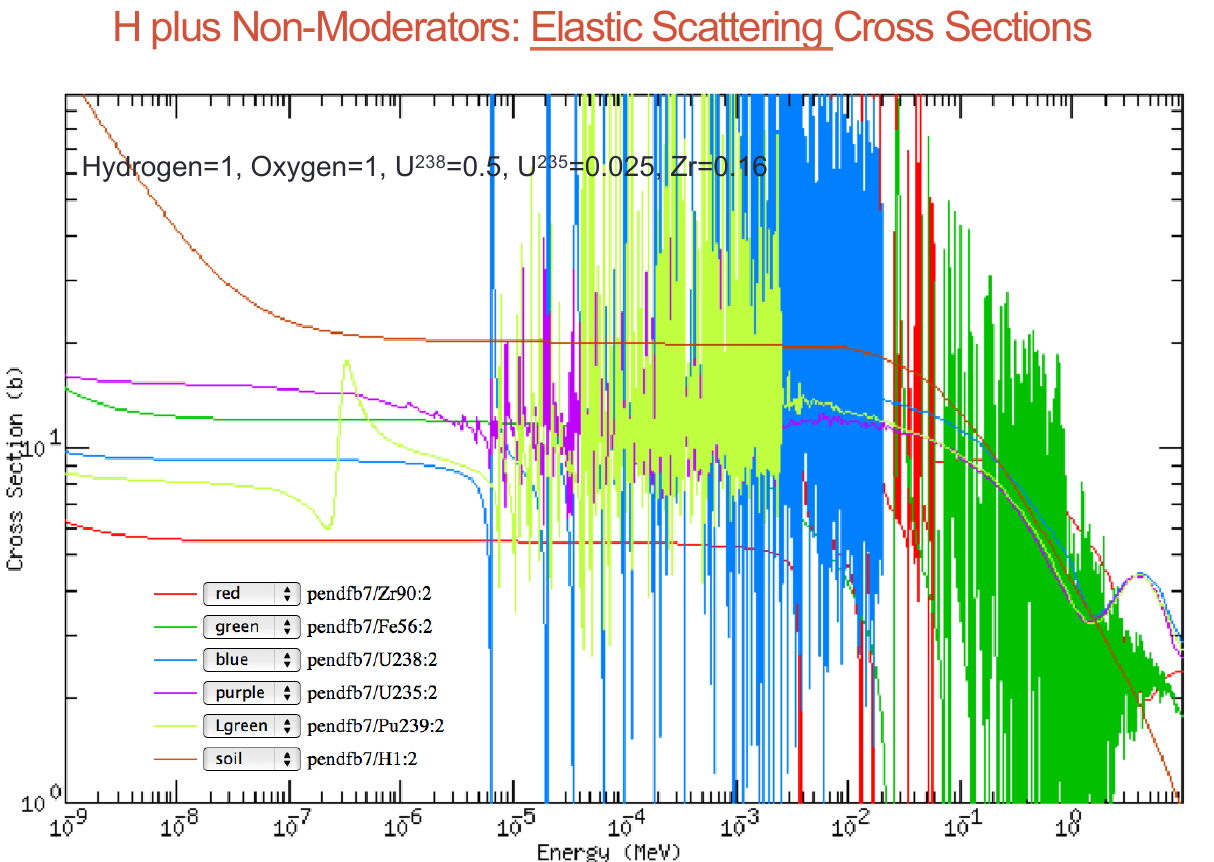
\includegraphics[width=4in]{images/scatter-xs-LWR.png}
  \caption{Elastic Scattering Cross Sections} \label{scatter-xs}
\end{figure}

\item Capture cross section as in Figure~\ref{capture-xs}: 
\begin{figure}
  \centering
  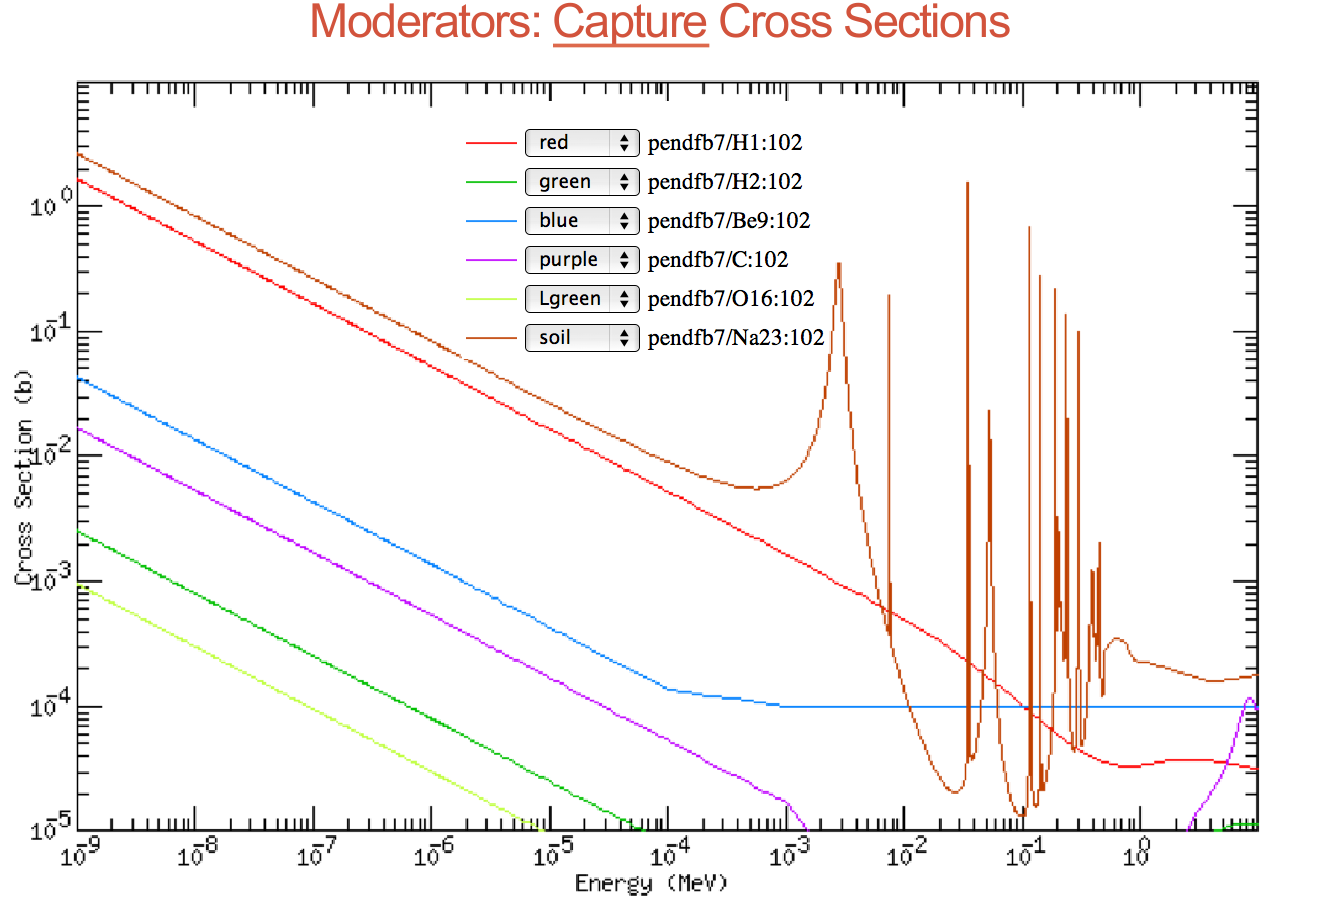
\includegraphics[width=4in]{images/capture-xs.png}
  \\
  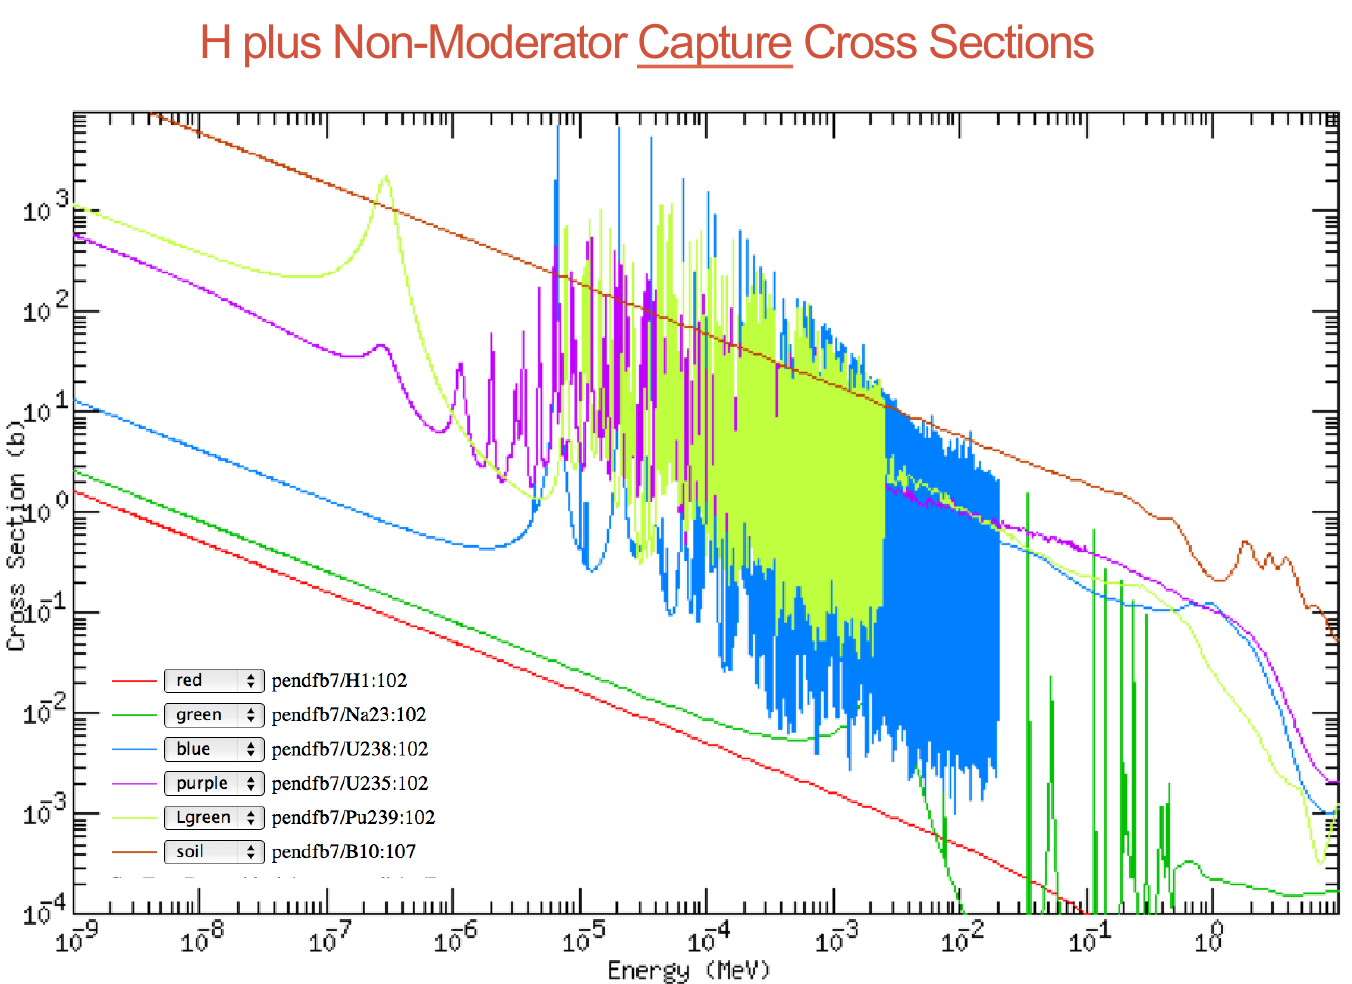
\includegraphics[width=4in]{images/capture-xs-2.png}
  \caption{Capture Cross Section} \label{capture-xs}
\end{figure}
\begin{enumerate}
\item H has no resonance; it has the highest scattering xs in LWR, so we can ignore any other isotopic's neutron scattering.   
\item Na has a huge resonance in 23 keV, and more resonances at higher energies because it is a heavy isotope.
\item Near zero energy,
\eqn{ \sigma(E\to 0) \propto \sqrt{\frac{kT}{AE}}    }
\item Resonance at 6 to 7 eV: U238. 
\item U235's thermal elastic xs is larger than 238's, and they both have resonance around the same range.   
\item A small resonance at .3 eV: Pu239 (its signiture is a super low energy scattering xs). 
\end{enumerate}

\item Given an unknown material type, all we care is to count the nucleus density of each material and look at it's xs. 
\item Average fission neutron energy: 2 MeV; average peak fission energy: 1 MeV; see fission sepctrum. 

\item Core decay heat after 1 day is about 1\% rated. 

\item Constants to know: 1u = 931.5 MeV. 
\end{enumerate}
%%%%%%%%%%%%%%%%%%%%%%%%% Qualify Exam End %%%%%%%%%%%%%%%%%%%%%%%%%%%%


\end{document}

% after exam 1:
\documentclass{school-22.211-notes}
\date{March 14, 2012}

\begin{document}
\maketitle

\lecture{Intro to Diffusion Theory}
\topic{Why We Need Deterministic Codes}
Lec10. Monte Carlo requires too much computing power. 


Pin-cell based, 


Assumbly based. 




In the next section we will discuss how to solve diffusion equation. 


\topic{k-infinity In Infinite Medium Calculations (No Leakage)}
Reference: Henry p. 104, Lec10 [FIXME] 
\eqn{ k_{\infty} =  \frac{\mbox{total fissions} \cdot \bar{\nu} }{\mbox{total absorptions}} = \frac{\int \dV \int \nu \overline{\Sigma_f} \Phi \dE}{\int \dV \int \overline{\Sigma_a} \Phi \dE} = \epsilon \eta f p }

\subtopic{k from one-group cross section}




\subtopic{k from two-group cross section}
\begin{enumerate}
\item General case: 
  \begin{align}
    \frac{\nu \overline{\Sigma_{f1}}}{\kinf} - \overline{\Sigma_{a1}} \phi_1 - \\
  \end{align}

\item Using effective removal cross section. We define an \hi{effective removal cross section} as,
  

   Although it looks like a chicken-to-egg problem that we include $\frac{\phi_2}{\phi_1}$ in $\hat{\Sigma}_{s12}$, my understanding is that we either know flux and needs to find cross section, or the other way around, hence we do not need to worry about this term. 

   If no upscattering, $\hat{\Sigma}_{s12}$ is effectively $\overline{\Sigma}_{s12}$, hence 
\end{enumerate}

\subtopic{k From Balance Equation}
For two region problem, we can also solve $\kinf$ from the neutron balance equation. 





The $\kinf$ from the three methods above should agree, because reaction rates conserves[FIXME].




\end{document}

\documentclass{school-22.211-notes}
\date{March 19, 2012}

\begin{document}
\maketitle

\lecture{One-Group Diffusion: Analytical Solutions, Part 1}
\topic{Helmholtz Equation}
We start with the one-group diffusion equation,
\eqn{ -\divergence D(\vecr) \gradient \phi(\vecr) + \Sigma_a(\vecr) \phi(\vecr) = \frac{1}{\keff} \nu \Sigma_f(\vecr) \phi(\vecr) }
Assume homogeneous material, that is, spatial constant cross section,
\eqn{ -D \laplacian \phi(\vecr) + \Sigma_a \phi(\vecr) = \frac{1}{\keff} \nu \Sigma_f \phi(\vecr) }
Rearranging and defining a buckling term, 
\eqn{ \laplacian \phi(\vecr) + \underbrace{\frac{ \frac{\nu \Sigma_f}{\keff} - \Sigma_a}{D} }_{B^2} \phi(\vecr) = 0 }
We obtain a classic Helmholtz Equation,
\eqn{ \boxed{\laplacian \phi(\vecr) + B_m^2 \phi(\vecr) = 0 } }
Helmholtz Equation implies that,
\eqn{ B_m^2 = - \frac{\laplacian \phi(\vecr)}{\phi(\vecr)} }
Notice,
\begin{enumerate}
\item Since $B_m^2$ is a constant, that is to say $\frac{\laplacian \phi(\vecr)}{\phi(\vecr)}$ is a constant, that is to say $\phi(\vecr)$ has a constant curvature. 
\item Material buckling: 
  \eqn{ B_m^2 = \frac{\frac{\nu \Sigma_f}{\keff} - \Sigma_a}{D} }
  which matches geometry buckling, 
  \eqn{ \keff = \frac{\nu \Sigma_f}{DB_g^2 + \Sigma_a} }
  where $DB^2_g$ is the leakage per unit volume per unit flux. Notice $\keff$ does not depend on volume or flux. 

\item Critical buckling: when a system is critical, the material buckling is uniquely determined by cross sections, 
  \eqn{ B_m^2 = \frac{\nu \Sigma_f - \Sigma_a}{D} = \frac{\frac{\nu \Sigma_f}{\Sigma_a} - 1}{\frac{D}{\Sigma_a}} = \frac{\kinf - 1}{M^2} }
  \hi{Migration area} $M^2 = \frac{D}{\Sigma_a}$ is a measurement of the amount of travelling before absorption. 


\item Solutions exist only for certain values of the buckling such that the flux is everywhere positive and vanishing on outer (or extrapolated) surfaces; we define these unique values as `geometrical buckling' $B_g^2$. The allowable values of geometrical buckling that satisfy the boundary conditions are uniquely determined reactor geometry.

\item For a criticality problem, we can solve find the $B^2$ such that the system is critical. Hence giving geometry, only certain materials would make the system critical; given material, only certain geometries would make the system critical. That is, given a reactor, it would be critical if and only if the material and the geometry satisfy,
  \eqn{ B_g^2 = B_m^2} 

\item Solution only exists when $\kinf > 1$ (exception: if there is external source, $\kinf$ can be less than 1 and the system is still critical). 


\end{enumerate}



Talbe~\ref{simple-geometry-laplacian} lists a couple of one group homogeneous geometry Laplacians. 
\begin{table}
  \centering
  \begin{tabular}{|l|l|} \hline
    Slab & $\dphidxn2 + B^2 \phi(x) = 0$ \\ \hline
    Sphere & $\dphidrn2 + \frac{2}{r} \dphidr + B^2 \phi(r) = 0$ \\ \hline
    Infinite Cylinder & $\dphidrn2 + \frac{1}{r} \dphidr + B^2 \phi(r) = 0$ \\ \hline
    Finite Cylinder & $\dphidrn2 + \frac{1}{r} \dphidr + \dphidzn2 + B^2 \phi(r,z) = 0$ \\ \hline
    Cartesian & $\dphidxn2 + \dphidyn2 + \dphidzn2 + B^2 \phi(x,y,z) = 0$ \\ \hline
  \end{tabular}
\caption{Simple Geometry Laplacians} \label{simple-geometry-laplacian}
\end{table}




\clearpage
\topic{One Group Criticality Problem}
 Slab $\in  \left[- \frac{L_0}{2}, \frac{L_0}{2} \right]$:
  \eqn{ \dphidxn2 + B^2 \phi (x) &= 0, &\phi(x) &= A \cos (Bx) + C \sin(Bx) }
BCs: $\phi(\pm L/2) = 0$, $\frac{L}{2} = \frac{L_0}{2} + 0.711 \lambda_{tr}$. Two equations two unknowns, 
  \eqn{ \left[ \begin{array}{cc} \cos(BL/2) & \sin(BL/2) \\ \cos(BL/2) & -\sin(BL/2) \end{array} \right] \left[ \begin{array}{cc} A \\ C \end{array} \right] = 0 }
  Set the determinant to be zero, we get $-2 \cos (BL/2) \sin (BL/2) = 0$. There are two possibilities: 
\eqn{ B_n&= \frac{n\pi}{L}  & \phi(x) &= \left\{ 
  \begin{array}{cc} 
    A_n \cos (B_n x) & n=1,3,5, \cdots \\
    A_n \sin (B_n x) & n=2,4,6, \cdots 
  \end{array} \right. }
But in order for $\phi(x) \ge 0$ everywhere, only $n=1$ is possible; that is, 
\eqn{ \phi(x) = A \cos \frac{\pi x}{L} }
and the criticality condition implies that, 
\eqn{ \frac{\nu \Sigma_f - \Sigma_a}{D}  = \left( \frac{\pi}{L} \right)^2 }

\begin{table}
  \small
  \makebox[\textwidth][c]{
  \begin{tabular}{|l|l|l|l|} \hline
    Geometry & Diffusion Equation & Flux & Geometrical Buckling \\ \hline
    Slab $\in  \left[- \frac{L}{2}, \frac{L}{2} \right]$ &$\dphidxn2 + B^2 \phi = 0$ & $\phi = A \cos \left( \frac{\pi x}{L} \right)$ & $B^2 = \left( \frac{\pi}{L} \right)^2$ \\ 
    Sphere $\in [0, R]$  & $\dphidrn2 + \frac{2}{r} \dphidr + B^2 \phi = 0$& $\phi= \frac{A}{r} \sin \left( \frac{\pi r}{R} \right)$ & $B^2 = \left( \frac{\pi}{R} \right)^2$ \\
    Cylinder ($z: \infty$) & $\dphidrn2 + \frac{1}{r} \dphidr + B^2 \phi = 0$ & $\phi = A J_0 \left( \frac{2.405 r}{R} \right)$ & $B^2 = \left( \frac{2.405}{R} \right)^2$ \\ 
    Cylinder (z: $\pm H/2$) & $\dphidrn2 + \frac{1}{r} \dphidr + \dphidzn2 + B^2 \phi = 0$ & $\phi = A J_0\left( \frac{2.405 r}{R} \right) \cos \left( \frac{\pi z}{H} \right)$ & $B^2 = \left( \frac{2.405}{R} \right)^2 + \left( \frac{\pi}{H} \right)^2$ \\ 
    Parallelepiped ($\pm \frac{L_i}{2}$) & $\dphidxn2 + \dphidyn2 + \dphidzn2 + B^2 \phi = 0$ & $\phi = A \cos \left( \frac{\pi x}{L_x} \right) \cos \left( \frac{\pi y}{L_y} \right) \cos \left( \frac{\pi x}{L_z} \right)$ & $B^2 = \left( \frac{\pi}{L_x} \right)^2 + \left( \frac{\pi}{L_y} \right)^2 + \left( \frac{\pi}{L_z} \right)^2$ \\ \hline
  \end{tabular}
}
  \caption{One Group Fundamental Mode Eigenvalues and Eigenvectors} \label{eigen-values}
\end{table}
\normalsize

Observations:
\begin{itemize}
\item The lowest node is the only one remains after the source is gone. 
\item For any positive value of materials buckling, there is a unique critical size for each reactor geometry. 
\item Example: know how to find height-to-diameter to minimize leakage. The optimal cylinder has a H/D of around 0.92. 
\end{itemize}


\clearpage
\topic{One Group Source Problem} \label{one-group-source-problem-subcritical}
Consider a subcritical multiplying medium, slab geometry from $-L/2$ to $L/2$, and with a source. 
\begin{align}
  - D \dphidxn2 + \Sigma_a \phi(x) &= \nu \Sigma_f \phi(x) + S(x) \\
  \dphidxn2 + B_m^2 \phi(x) &= -\frac{S(x)}{D} 
\end{align}
Because $B^2 = \frac{\nu \Sigma_f - \Sigma_a}{D} < 0 $ for a subcritical condition, we can re-write $B^2 = - |B|^2$,
\eqn{ \dphidxn2 - |B|^2 \phi(x) = \tilde{S}(x) }
The general/homogeneous solution is,
\eqn{ \phi_H (x) = A e^{|B|x} + Ce^{-|B|x} = A \cosh (|B|x) + C \sinh (|B| x) }
The particular solution depends on source $\tilde{S}(x)$. Apply BCs $\phi \left( \pm \frac{L}{2} \right) = 0$, we get the boundary conditions in the matrix form,
\eqn{ \left[ \begin{array}{cc} 
\cosh(|B|L/2) & \sinh(|B|L/2) \\
\sinh(|B|L/2) & \cosh(|B|L/2) 
\end{array} \right] 
\left[ \begin{array}{c}
A \\ C \end{array} \right] 
= - \left[ \begin{array}{c} 
\phi_p(L/2) \\ \phi_p(-L/2) \end{array} \right] }
Interpretations:
\begin{enumerate}
\item Coefficients A and C are uniquely determined for given source distribution; 
\item There always exists a physically realizable solution (no critical buckling!);
\item In the limit of $S\to 0$, the only physical solution is the trivial solution (\textcolor{red}{shouldn't the only solution be the general solution?}). 
\end{enumerate}

\end{document}

\documentclass{school-22.211-notes}
\date{March 21, 2012}

\begin{document}
\maketitle

\lecture{One-Group Diffusion: Source Problem} \label{1g-source}
We are going to cover some classical examples to understand the mechanics, boundary conditions, and interface conditions. Know these for the exam. 

\begin{enumerate}
\item For a non-multiplying medium ($\Sigma_f = 0$), and assume that $D, \Sigma_a$ are constant in space, we arrive at the \hi{inhomogeneous Helmholtz Equation}, 
\eqn{ - D \laplacian \phi (\vecr) + \Sigma_a \phi (\vecr) = S(\vecr) }
We define the diffusion length as $\displaystyle L = \sqrt{\frac{D}{\Sigma_a}}$, then the balance equation becomes, 
\eqn{ - \laplacian \phi (\vecr) + \frac{1}{L^2} \phi(\vecr) = \frac{S(\vecr)}{D} }

\item For a multiplying medium, we typically use $\displaystyle B^2 = \frac{\frac{\nu \Sigma_f}{\keff} - \Sigma_a}{D}$. 

\item Recap:
\eqn{ \laplacian \phi(\vecr) + B_m^2 \phi(\vecr) &= \laplacian \phi(\vecr) - \frac{1}{L^2} \phi(\vecr)= - \frac{S}{D} & B_m^2 = -\frac{1}{L^2} = \frac{\nu \Sigma_f - \Sigma_a}{D} 
\label{bal-eqn}}
\end{enumerate}





\clearpage
\topic{Arbitrary Source in Finite Multiplying Medium} \label{one-group-source-problem-subcritical}
Consider a subcritical multiplying medium, slab geometry from $-L/2$ to $L/2$, and with a source. 
\begin{align}
  - D \dphidxn2 + \Sigma_a \phi(x) &= \nu \Sigma_f \phi(x) + S(x) \\
  \dphidxn2 + B_m^2 \phi(x) &= -\frac{S(x)}{D} 
\end{align}
Given $\Sigma_a > \nu \Sigma_f$, $B^2 = \frac{\nu \Sigma_f - \Sigma_a}{D} < 0 $, we re-write $B^2 = - |B|^2$,
\eqn{ \dphidxn2 - |B|^2 \phi(x) = \tilde{S}(x) }
The general/homogeneous solution is,
\eqn{ \phi_H (x) = A e^{|B|x} + Ce^{-|B|x} = A \cosh (|B|x) + C \sinh (|B| x) }
The particular solution depends on source $\tilde{S}(x)$. Apply BCs $\phi \left( \pm \frac{L}{2} \right) = 0$, we get the boundary conditions in the matrix form,
\eqn{ \left[ \begin{array}{cc} 
\cosh(|B|L/2) & \sinh(|B|L/2) \\
\sinh(|B|L/2) & \cosh(|B|L/2) 
\end{array} \right] 
\left[ \begin{array}{c}
A \\ C \end{array} \right] 
= - \left[ \begin{array}{c} 
\phi_p(L/2) \\ \phi_p(-L/2) \end{array} \right] }
Coefficients A and C are uniquely determined for a given source distribution: 
\begin{itemize}
\item There always exists a physically realizable solution (no critical buckling!);
\item In the limit of $S\to 0$, the only physical solution is the trivial solution. 
\end{itemize}




\clearpage
\topic{Plane Source in Finite Multiplying Medium with $\kinf < 1$}
Consider a finite multiplying medium, $\kinf < 1$, a slab geometry from $0$ to $H$, and a plane source at $0$.  
\eqn{ B_m^2 = \frac{\nu \Sigma_f - \Sigma_a}{D} &= \frac{k_{\infty} - 1}{L^2} < 0, & B_m^2 &\to -|B_m|^2}
\begin{enumerate}
\item For the homogeneous solution, we assume there is no source, 
\eqn{\dphidxn2 - |B_m|^2 \phi &= 0, &\phi(x) &= A\cosh(|B_m|x) + B \sinh(|B_m|x) }

\item BC 1: $\displaystyle \phi(0) = \phi_0, \phi(H) = 0$, we can solve for the coefficients, 
\eqn{ \boxed{\phi(x) = \phi_0 \left[ \cosh(|B_m|x) - \frac{\cosh(|B_m|H)}{\sinh(|B_m|H)} \sinh(|B_m|x) \right] } }

\item Extreme condition: if we let the size of the slab to go to infinity, 
\eqn{\lim_{H \to \infty} \phi(x) = \phi_0 [\cosh(|B_m|x) - \sinh(|B_m|x)] = \phi_0 e^{-|B_m|x} = \frac{S_0L}{2D} e^{-|B_m|x} }



\item Notice in both finite and infinite case, the fluxes have convex shapes; the finite curve is below the infinite curve though. 
\begin{figure}[ht]
  \centering
  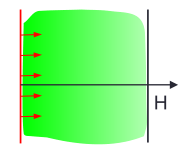
\includegraphics[width=2.5in]{images/dfs/plane-multiplying-geo.png}
  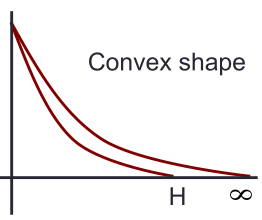
\includegraphics[width=2.5in]{images/dfs/plane-multiplying-phi.png}
  \caption{Plane Source in Finite Multiplying Medium with $\kinf < 1$}
\end{figure}
\end{enumerate}


\clearpage
\topic{Plane Source in Finite Multiplying Medium with $\kinf > 1$}
Consider a finite multiplying medium with $\kinf > 1$, it is a slab extending from $-H/2$ to $H/2$, it is subcritical with leakage, BC are from the current at center and the zero flux at the H/2 boundary. 
\eqn{ \dphidxn2 + B_m^2 \phi &= 0,  & B_m^2 &= \frac{\nu \Sigma_f - \Sigma_a}{D} = \frac{\kinf - 1}{L^2} > 0  &\phi(x) &= A \cos(B_mx) + B\sin(B_mx) }
BC1: $\phi(H/2) = 0$; BC2: $J(0) = \frac{S_0}{2}$. We can solve for the coefficients, and place absolute sign to represent the whole geometry: 
\eqn{ \phi(x) = \frac{S_0}{2DB_m \cos\left( \frac{B_m H}{2} \right)} \sin\left[ B_m \left(\frac{H}{2} - |x|\right) \right] }
Interpretations:
\begin{enumerate}
\item Because $\kinf > 1$, the flux shape is concave, that is, increasing negative slopes in the positive domain. In Fig.~\ref{approach-critical}, flux is convex when $\kinf < 1$ and concave when $\kinf > 1$, until we hit the cosine shape when $\keff = 1, \kinf = 1 + B^2L^2$ from 
  \eqn{ B^2 &= \frac{\frac{\nu \Sigma_f}{\keff} - \Sigma_a}{D} = \frac{\frac{\kinf}{\keff} - 1}{L^2}  & \kinf &= \keff + B^2 L^2}
\item If $H$ is increased to the critical dimension, that is, $H \to \frac{\pi}{B_m}$, then $\phi(0) \to \infty$; that is, if the reactor is critical, the flux at the source is infinite. That is, there is no steady-state solution for flux at the source site. In fact, if we place a fission detector at $x=0$ and measure source multiplication, 
  \eqn{M_s(0) = \frac{N_d \sigma_{f,d} V_d \phi(0)}{S_0} \propto \frac{\sigma_f}{2DB} \tan\left(\frac{BH}{2} \right) }
  Or the inverse source multiplication factor, 
  \eqn{ \frac{1}{M_s(0)} \propto \frac{1}{\tan\left(\frac{BH}{2} \right)} \to 0 }
\item To reach criticality, we can add fuel elements, withdraw control rods, and dilute boron. 1/M is useful for estimating criticality as shown in Figure~\ref{approach-critical}. 
  \begin{figure}[ht]
    \centering
    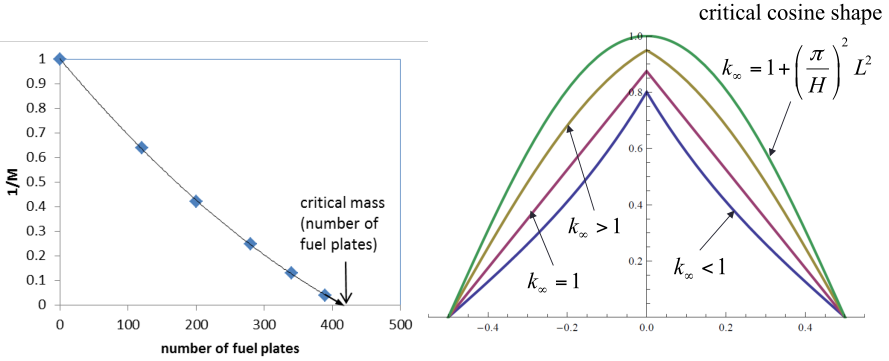
\includegraphics[width=5in]{images/dfs/approach-critical.png}
    \caption{1/M plot and Flux Shape In Approaching Criticality}\label{approach-critical}
  \end{figure}
\end{enumerate}




\clearpage
\topic{Summary}
\begin{enumerate}
\item \textbf{Super-positioning of sources}: if we are given a random source that is the sum of a couple of common forms of sources, we can super-position the flux from each of the common sources. This method works in any non-multiplying medium, and in multiplying medium in subcritical condition\footnote{Supercritical condition, as source increaes, flux inverts}. For instance, we can super-position point sources to get a line source. 

\item Diffusion theory is valid: 
  \begin{itemize}
    \item when there is little geometry heterogeneity;
    \item when $\Sigma_a \ll \Sigma_s$;
    \item when position is not too close to interface and source.
  \end{itemize}
  Diffusion theory is not valid near singularities. 

\item $\kinf$ is important\footnote{know this for the exams}: 
  \begin{itemize}
  \item $\kinf = 1$: flux is straight line;
  \item $\kinf < 1$ means $B^2 < 0$, flux is $\sinh, \cosh$ which is convex; 
  \item $\kinf > 1$ means $B^2 > 0$, flux is $\sin, \cos$ which is concave. 
  \end{itemize}
\end{enumerate}

  \begin{table}[ht]
    \centering
    \begin{tabular}{|c|c|c|c|c|} \hline
      Source & Geometry & Material &BCs & Flux \\ \hline \hline
      Point & $\infty$ Sphere & Non-multi.  & $\displaystyle \lim_{r\to\infty} \phi = 0, \lim_{r\to 0} 4 \pi r^2 J(r) = S_0$ & $\displaystyle \frac{S_0}{4\pi D} \frac{e^{-r/L}}{r}$ \\ \hline
      Plane & $\infty$ Slab & Non-multi. &$\displaystyle \lim_{x\to \infty} = 0, \lim_{x \to 0} J(x)  = \frac{S_0}{2}$ & $\displaystyle \frac{S_0 L}{2D} e^{-|x|/L}$ \\ \hline
      Plane & Finite Slab &Multi. $\kinf < 1$ & $\phi(0) = \phi_0, \phi(H) = 0$ & $\displaystyle \phi_0 \left[ \cosh(|B|x) - \coth(|B|H) \sinh(|B| x) \right]$ \\ \hline
      Plane & Finite Slab &Multi. $\kinf > 1$ & $\displaystyle \phi(H/2) = 0, J(0) = \frac{S_0}{2}$ & $\displaystyle \frac{S_0}{2D B_m \cos (BH/2)} \sin \left[ B \left( \frac{H}{2} - |x| \right) \right]$ \\ \hline
    \end{tabular}
    \caption{Subcritical System: Source and Flux} 
  \end{table}
  
  
\end{document}

\documentclass{school-22.211-notes}
\date{April  2, 2012}

\begin{document}
\maketitle

\lecture{Two-Group Diffusion: Numerical Solutions}
\topic{Simple Numerical Methods to Solve Diffusion Equations}
\subtopic{Derivation of Neutron Balance Equation}
Recall the two-group neutron balance equations:
\begin{itemize}
\item Total fission source is: 
  \eqn{S_f(r) = \mu \Sigma_{f1} (r) \phi_1 (r) + \mu \Sigma_{f2} (r) \phi_2(r) }
  $\xi_1 = 1, \xi_2 = 0$ which implies that fission source in the thermal group is zero.
\item Scattering source: we define effective down-scattering, so up-scattering is zero $\Sigma_{21}(r) = 0$. 
\item Two-group diffusion equations: 
\eqn{-\gradient D_1 \divergence \phi_1 + [\Sigma_{a1} + \Sigma_{s12}] \phi_1 = \nu \Sigma_{f1} \phi_1 + \nu \Sigma_{f2} \phi_2 + S_1} 
\eqn{-\gradient D_2 \divergence \phi_2 + \Sigma_{a2} \phi_2 = \Sigma_{s12} \phi_1 + S_2}
\end{itemize}

\subtopic{Derivation of Interface Flux}
Then we construct a finite spatial mesh in which cross sections are constant; integrate the neutron diffusion equations over each mesh cell $\Delta^n$,
\eqn{-\int \ddx D_1^n \ddx \phi_1^n \dx + \Sigma_{r1}^n  \phi_1^n \Delta^n = \nu \Sigma_{f1}^n \phi_1^n \Delta^n + \nu \Sigma_{f2}^n \phi_2^n \Delta^n + S_1 \Delta^n} 
\eqn{-\int \ddx D_2^n \ddx \phi_2^n  \dx + \Sigma_{a2}^n \phi_2^n \Delta^n = \Sigma_{s12}^n \phi_1^n \Delta^n + S_2 \Delta^n}
We evaluate the integral term\footnote{Lectuer says use the divergence theorem $\int \divergence \vec{F} \dV = \int_S \vec{F} \cdot \vec{n} \dS$, I think this is just manipulating integral and $\int \ddx A \dx \to A$}, 
\eqn{\int \ddx D_1^n \ddx \phi_1^n \dx  = \left. D_1^n \ddx \phi_1^n \right|_{n^+} - \left. D_1^n \ddx \phi_1^n \right|_{n^-} }
Then we have,
\eqn{\left. D_1^n \ddx \phi_1^n \right|_{n^-} - \left. D_1^n \ddx \phi_1^n \right|_{n^+} + \Sigma_{r1}^n  \phi_1^n \Delta^n = \nu \Sigma_{f1}^n \phi_1^n \Delta^n + \nu \Sigma_{f2}^n \phi_2^n \Delta^n + S_1 \Delta^n} 
\eqn{\left. D_2^n \ddx \phi_2^n \right|_{n^-} - \left. D_2^n \ddx \phi_2^n \right|_{n^+} + \Sigma_{a2}^n \phi_2^n \Delta^n = \Sigma_{s12}^n \phi_1^n \Delta^n + S_2 \Delta^n}
We notice that the $-D \ddx \phi$ terms are just flux terms (in fact, they are the interface fluxes):
\eqn{J_n^+ = - \left. D_g^n \ddx \phi_g^n \right|_{n+} = -D_g^n \frac{\phi_g^S - \phi_g^n}{\Delta/2} }
\eqn{J_n^- = - \left. D_g^{n+1} \ddx \phi_g^{n+1} \right|_{n-} = - D_g^{n+1} \frac{\phi_g^{n+1} - \phi_g^s}{\Delta/2} }
By continuity of the net current, we can set the above two equations to equal to each other, 
\eqn{  -D_g^n \frac{\phi_g^S - \phi_g^n}{\Delta/2} =  - D_g^{n+1} \frac{\phi_g^{n+1} - \phi_g^s}{\Delta/2} }
From where we can solve for the interface flux, 
\eqn{ \phi_g^s = \frac{D_g^{n+1} \phi_g^{n+1} + D_g^n \phi_g^n}{D_g^n + D_g^{n+1}}} 
Then we can get th net current in terms of mesh fluxes: 
\eqn{ J_n^+ = - \frac{2D_g^n}{\Delta} \left[ \frac{ D^{n+1} \phi^{n+1} + D^n \phi^n}{D^n + D^{n+1}} - \phi^n \right] = - \overbrace{\frac{2 D^n D^{n+1} }{\Delta (D^n + D^{n+1})}}^{\to \hat{D}^{n,n+1}} (\phi^{n+1} - \phi^{n}) }
That is, 
\eqn{J_n^+ &= - \hat{D}^{n,n+1} (\phi^{n+1} - \phi^n)  & J_n^- &= - \hat{D}^{n-1, n} (\phi^n - \phi^{n-1} ) \label{net-current}}


\subtopic{Derivation of Finite Difference Equations}
Plug Eq.~\ref{net-current} back into diffusion equations, we get, 
\eqn{ \hat{D}_1^{n-1,n} (\phi_1^n - \phi_1^{n-1})  - \hat{D}_1^{n,n+1} (\phi_1^{n+1} - \phi_1^n) + \Sigma_{r1}^n \phi_1^n \Delta^n &= \mu \Sigma_{f1}^n \phi_1^n \Delta^n + \mu \Sigma_{f2}^n \phi_2^n \Delta^n + S_1 \Delta^n} 
\eqn{ \hat{D}_2^{n-1,n} (\phi_2^n - \phi_2^{n-1})  - \hat{D}_2^{n,n+1} (\phi_2^{n+1} - \phi_2^n) + \Sigma_{a2}^n \phi_2^n \Delta^n &= \Sigma_{s12}^n \phi_1^n \Delta^n + S_2 \Delta^n} 
Rearranging terms by fluxes, we get, 
\eqn{ - \hat{D}_1^{n-1,n} \phi_1^{n-1} - \hat{D}_1^{n,n+1} \phi_1^{n+1} + [ \Sigma_{r1}^n \Delta^n + \hat{D}_1^{n-1, n} + \hat{D}_1^{n,n+1} ] \phi_1^n = \nu \Sigma_{f1}^n \phi_1^n \Delta^n + \nu \Sigma_{f2}^n \phi_2^n \Delta^n + S_1^n \Delta^n} 
\eqn{ - \hat{D}_2^{n-1,n} \phi_2^{n-1} - \hat{D}_2^{n,n+1} \phi_2^{n+1} + [\Sigma_{a2}^n \Delta^n + \hat{D}_2^{n-1.n} + \hat{D}_2^{n,n+1} ] \phi_2^n = \Sigma_{s12}^n \phi_1^n \Delta^n + S_2^n \Delta^n }


\subtopic{Derivation of Boundary Condition}
Interior of the geometry, the boundary conditions are implied. The exterior boundaries have to be specified. There are two types of boundary conditions:
\begin{enumerate}
\item Zero Flux BC: 
\eqn{ J_g^N = -D_g^N \frac{ -\phi_g^N - \phi_g^N}{\Delta^N}  = \frac{2 D_g^N}{\Delta^N} \phi_g^N }
\item Zero Incoming Current BC:
\eqn{ J^- = \frac{1}{4} \phi - \frac{1}{2} J_n = 0 }
which implies,
\begin{align}
  J_g^N &= \frac{\phi_g^s}{2} = -D_g^N \frac{\phi_g^s - \phi_g^N}{\Delta/2} \\
  &= - \frac{2 D_g^N}{\Delta^N} \frac{\frac{2D_g^N}{\Delta^N} - 1}{\frac{1}{2} + \frac{2D_g^N}{\Delta}} \phi_g^N \\
  &= \boxed{ \frac{2D_g^N}{\Delta^N} \left[ \frac{1}{1 + \frac{4 D_g^N}{\Delta^N}} \right] \phi_g^N } \label{JgN}
\end{align}
In Eqn.~\ref{JgN}, if $D \to 0$, we get zero flux boundary condition; if $D \to \infty$, we get zero current boundary condition. 
\end{enumerate}


\topic{Matrix Representation of 1D Slab Diffusion Equations}
\subtopic{Construct Matrix}
If we use $L$ for the $\phi^{n-1}$ term, $U$ for the $\phi^{n+1}$ term, $D$ for the $\phi^n$ term, $T$ for the transport term, we can express the finite difference equation in matrix form as: 
\begin{align}
[L_1 + D_1 + U_1] [\phi_1] &= [M_1] [\phi_1] + [M_2][\phi_2] + [S_1] \\
[L_2 + D_2 + U_2] [\phi_2] &= [T_2] [\phi_1] + [S_2] 
\end{align}
We define a vector of group fluxes, 
\begin{align}
\left[ \begin{array}{cc} 
[L_1 + D_1 + U_1] & [0] \\
-[T_2] & [L_2 + D_2 + U_2] \\
\end{array} \right] 
\left[ \begin{array}{c}
\phi_1 \\ \phi_2 \\ \end{array} \right] 
= \left[ {\begin{array}{cc} \left[M_1\right] & \left[M_2\right] \\ \left[0\right] & \left[0\right] \end{array}} \right] 
\left[ \begin{array}{c}
\phi_1 \\ \phi_2 \\ \end{array} \right] 
+ 
\left[ \begin{array}{c} 
S_1 \\ S_2 \\ \end{array} \right] 
\end{align}
Whose compressed form is, 
\eqn{ [A] [\phi] = [M] [\phi] + [S] }
The two matrix are plotted in Figure~\ref{matrix-form}. Notice there are missing points in A; explaination: Block matrix: there is no coupling of group 1 left flux to the group 2 right flux. 
\begin{figure}
  \centering
  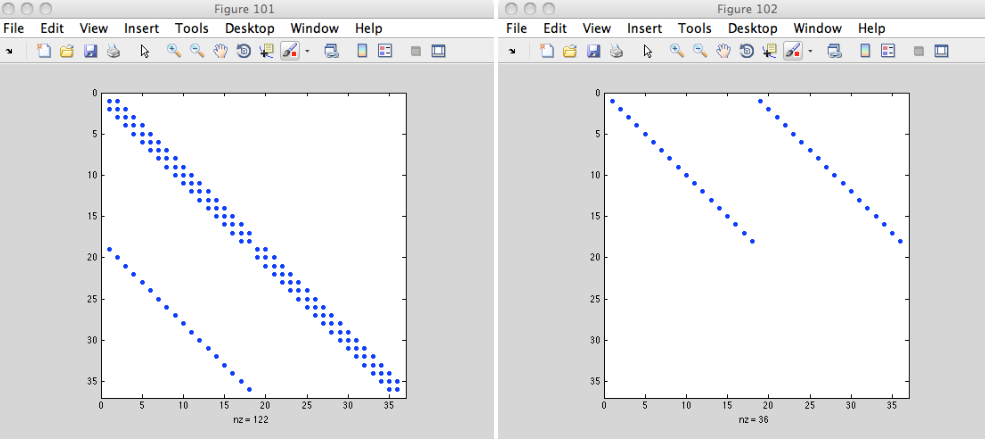
\includegraphics[width=4in]{images/dfs/matrix-form.png}
  \caption{Destruction and Production Matrix} \label{matrix-form}
\end{figure}


\subtopic{Method 1: Sequential Source/Fixed-Source Problem}
\begin{align}
[A] [\phi] &= [M] [\phi] + [S] \\
[A - M ] [\phi] &= [S] \\
[\phi] &= [A - M]^{-1} [S]
\end{align}
In this method, we guess $\keff$, and given a source we can solve for the flux. We never solve real questions this way, because 

If we have a super-critical problem, then the only way to get criticality with an additional source is through negative flux. 

A reactor is like an amplifier; the closer it is to criticality the more amplification it is; when critical, the amplification is infinity. 


\subtopic{Method 2: Direct Matlab Eigenvalue Solver}
We can solve for $\keff$ directly from: 
\begin{align}
[A] [\phi] &= \frac{1}{\keff} [M] [\phi] \\
[A]^{-1} [M] [\phi] &= \keff [\phi]
\end{align}
Notice that the eigenvectors are arbitrarily normalized; hence it is fine if the flux is negative. 



\subtopic{Method 3: Power Iterations}
\begin{align}
[A] [\phi]^{n+1} &= [M] [\phi]^n \\
\keff &= \frac{[M][\phi]^{n+1} }{[M] [\phi]^n} 
\end{align}
The rate our fission source converges depends on material, geometry etc. \hi{The dominance ratio} is defined as $\frac{\lambda_1}{\lambda_2}$; and it is 0.97 for this example. If we know the dominance ratio of the problem, we can estimate the number of iterations needed to converge. 
\begin{figure}
  \centering
  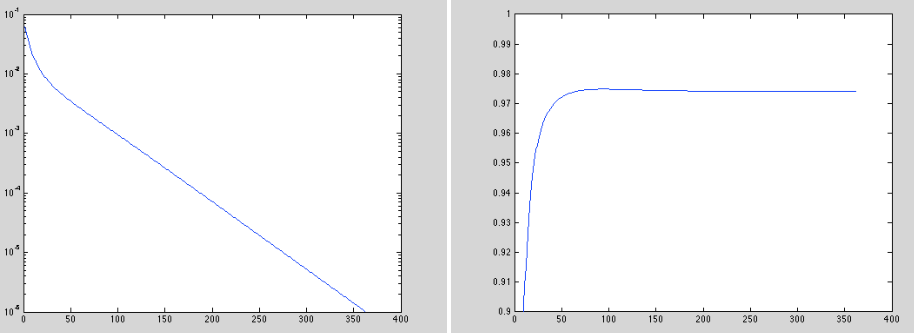
\includegraphics[width=4in]{images/dfs/power-iteration-convergence.png}
  \caption{The Convergence Rate of Power Iteration}
\end{figure}

\subtopic{Method 3+: Power Iterations with Gauss-Jacobi Numerical Inversion of Flux Matrix}
See Lec. 12 slide 21. In a steady-state problem, it does not matter whether we fully converge our flux iteration. 


\topic{HW5: Numerical Solution of Solving Two-Group Diffusion Problems}
It is not just iterative convergence that we care; spatial convergence is required as well. 

\topic{Summary}
Remember for real 3D problem,
\begin{itemize}
\item Matrix inversion if of order $N^3$, so in real applications no matrix inversion;
\item Finding all eigenvalues if at least order $N^2$;
\item Iterative inversion must be order $N$ to be practical for large problems;
\item Multi-level iteration is a practical necessity. 
\end{itemize}


\end{document}

\documentclass{school-22.211-notes}
\date{April  4, 2012}

\begin{document}
\maketitle

\lecture{Two-Group Diffusion: Analytical Solutions}
We are going to cover six classical examples to understand the mechanics, boundary conditions, and interface conditions. Know these for the exam. 
\topic{Point Source in Infinite Non-Multiplying Medium}


\topic{Plane Source in Infinite Non-Multiplying Medium}


\topic{Plane Source in Finite Multiplying Medium with $\kinf < 1$}




Notice in both finite and infinite case, the fluxes are convex; the finite curve is under the infinite curve. 



\topic{Plane Source in Finite Multiplying Medium with $\kinf > 1$}



If the reactor is critical, the flux at the source is is infinite. That is, there is no steady-state solution for flux at the source site. 



\topic{Critical Finite Cube}



\topic{Critical Finite Cylinder} 



\topic{Critical Reflected Slab Reactor}



\topic{Summary}
\begin{enumerate}
\item \textit{Super-positioning of sources}: if we are given a random source that is the sum of a couple of common forms of sources, we can super-position the flux from each of the common sources. This method works in any non-multiplying medium, and in multiplying medium in subcritical condition\footnote{Supercritical condition, as source increaes, flux inverts}. For instance, we can super-position point sources to get a line source. 
\item Diffusion theory is not valid near singularities. 
\item $\kinf$ is important\footnote{know this for the exams}: 
  \begin{enumerate}
  \item $\kinf = 1$: flux is straight line;
  \item $\kinf < 1$ means $B^2 < 1$, flux is $\sinh, \coshn$ which is convex; 
  \item $\kinf > 1$ means $B^2 > 0$, flux is $\sin, \cos$ which is concave. 
  \item Know how to get the critical buckling for different geometries. 
  \item Seperation of variables works as long as there is no one more than one direction that is heterogeneous. 
  \end{enumerate}

  \begin{table}
    \centering
    \begin{tabular}{|c|c|c|} \hline
      Source & Geometry & Flux \\ \hline \hline
      Point & Infinite Slab & \\ \hline
    \end{tabular}
    \caption{Subcritical System: Source and Flux} 
  \end{table}
  
  
\end{document}

% after exam 2:
\documentclass{school-22.211-notes}
\date{April  9, 2012}

\begin{document}
\maketitle

\lecture{Fission Product Poisoning} \label{fission-product-poisoning}
\topic{Fission Product Chain}
\begin{figure}[ht]
  \centering
  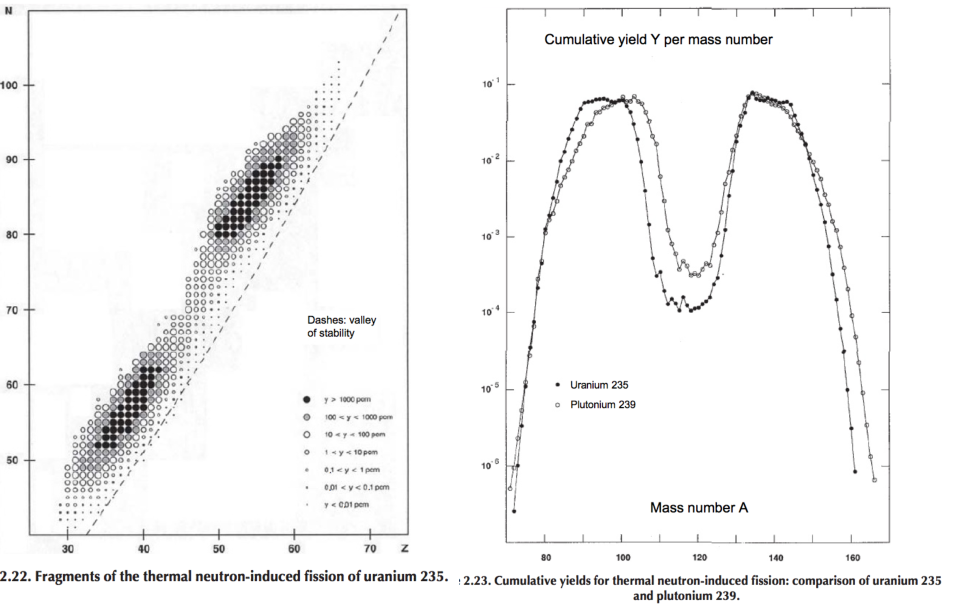
\includegraphics[width=5in]{images/dfs/fission-product-yield.png}
  \caption{Fission Product Yields, Fission Fragments}
\end{figure}

The fission products have the following properties: 
\begin{enumerate}
\item Number: almost all fissions produce precisely two fission produces per fission;
\item Unstability: most fission products are highly unstable and radially decay to other nuclides;
\item Thermal spectrum: some fission produces have large thermal absorption cross sections, which are important for thermal spectrum reactors as in Figure~\ref{major-capture};
\item Fast spectrum: fast reactors are much less sensitive to fission products, because thermal spectrum does not matter. 
\item Distribution: contributing factors are: which species are fissioned (U235, Pu239, etc), the incident fission neutron energy, random statistical fluctuations nuclide breakup.
\item Independent fission yield is a different concept from the cumulative fission yield: the former only accounts for fission yield, whereas the latter accounts for generation of the isotope from independent yield as well as all the precursor isotopes that decay into a specific isotope. 
\item Meda-stable state: an isotope may not directly decay into a stable state; it may branch into a meda-stable state. For our purpose, we are going to take the simplified approach.
\end{enumerate}
\begin{figure}
  \centering
  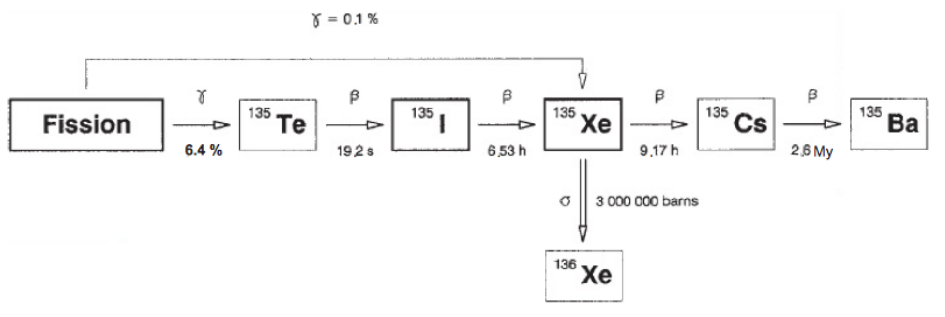
\includegraphics[width=5in]{images/dfs/Xe135.png}
  \caption{I135/Xe135 Chain} \label{Xe135} 
\end{figure}

As an example, we look at the Xenon-135 Chain in Figure~\ref{Xe135}. Typically very rapid transitions are not followed in details when modeling reactor behavior. For instance, because Te's half-life is 19s, we can assume that \ce{^{135}I} is producted instantenously. Most of the chains are similar and are dominated by beta decays until they are stable. 

\begin{figure}
  \centering
  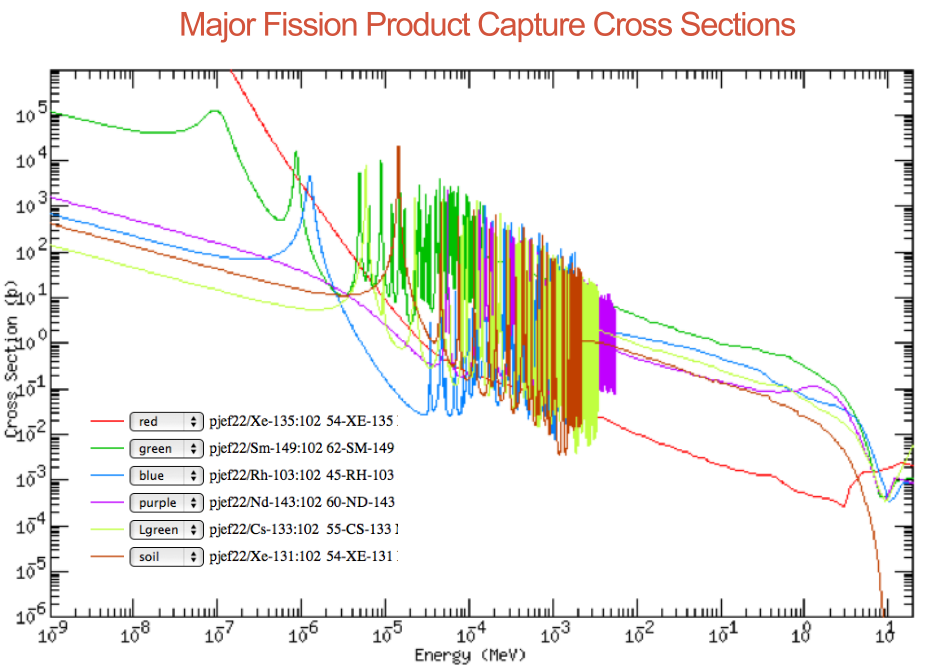
\includegraphics[width=0.59\textwidth]{images/dfs/fission-product-capture-xs.png}
  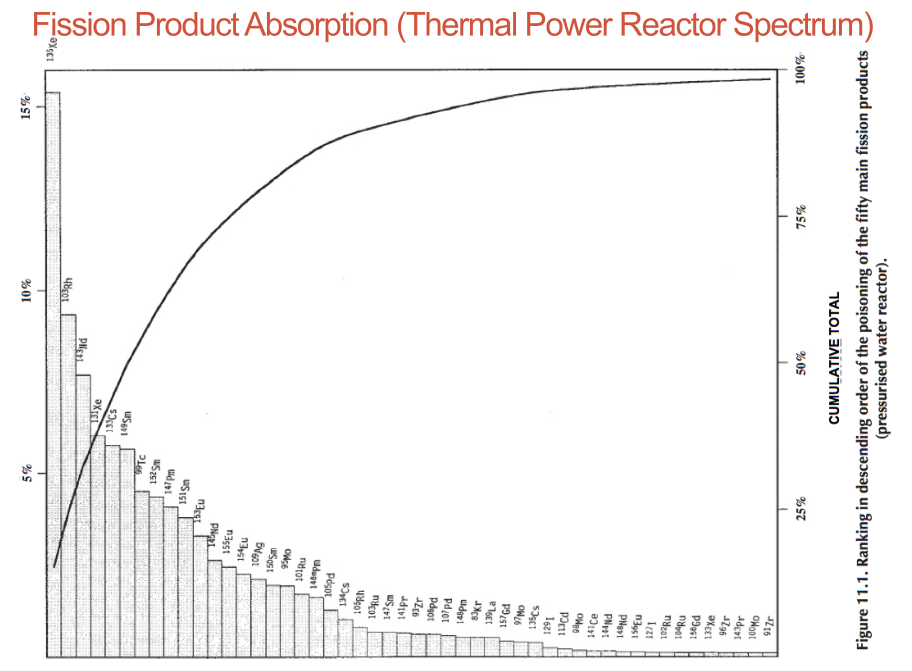
\includegraphics[width=0.59\textwidth]{images/dfs/fission-product-absorption.png}
  \caption{Major Fission Products Absorption} \label{major-capture} 
\end{figure}


\clearpage
\topic{Nuclide Depletion Equation/Neutron Balance Equation}
The numerical solution of nuclide depletion equation is:
\begin{align}
\dNdt + A(t) N(t) &= Y \\
\mbox{IF} &= e^{\int A(t) \dt} = e^{At} \\
e^{At} \dNdt + e^{At} A(t) N(t) &= e^{At} Y \\
\ddt[e^{At} N(t) ] &= e^{At} Y \\
e^{At} N(t) &= A^{-1} e^{At} Y + C 
\end{align}
Using the particular solution that $N_0 = N(t=0)$, then 
\eqn{ N_0 = A^{-1} Y + C \Rightarrow C = N_0 - A^{-1} Y } 
\eqn{ e^{At} N(t) = A^{-1} [e^{At} Y - Y ] + N_0 }
\eqn{ \boxed{ N(t) = e^{-At} N_0 + e^{-At} A^{-1} [e^{At} Y - Y ] } }
We can also write the above differential equation into the matrix form as in Figure~\ref{depletion-matrix}. Notice we asume fission yields, cross sections, and fluxes are constant over the time interval $t_{n-1}, t_n$,
\eqn{ [N(t_n)] = e^{-[A] \Delta t_n} [N(t_{n-1})] + e^{-[A]\Delta t_n} [A]^{-1} [e^{[A] \Delta t_n} Y - Y ] }
\begin{figure}[ht]
  \centering
  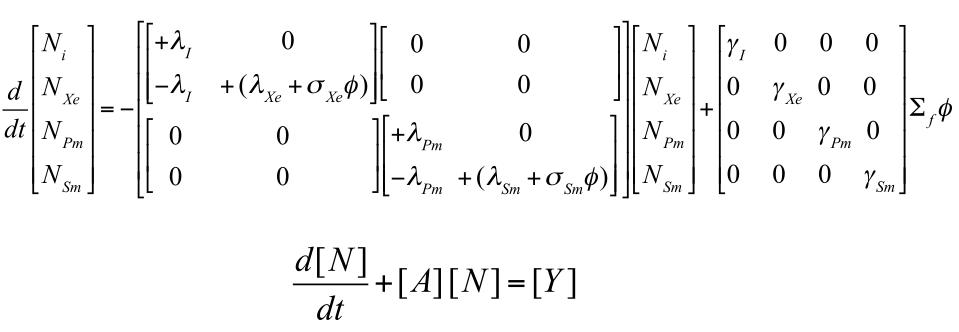
\includegraphics[width=5in]{images/dfs/depletion-matrix-form.png}
  \caption{Nuclide Depletion Equations in Matrix Form} \label{depletion-matrix} 
\end{figure}

\clearpage
\begin{figure}[ht]
  \centering
  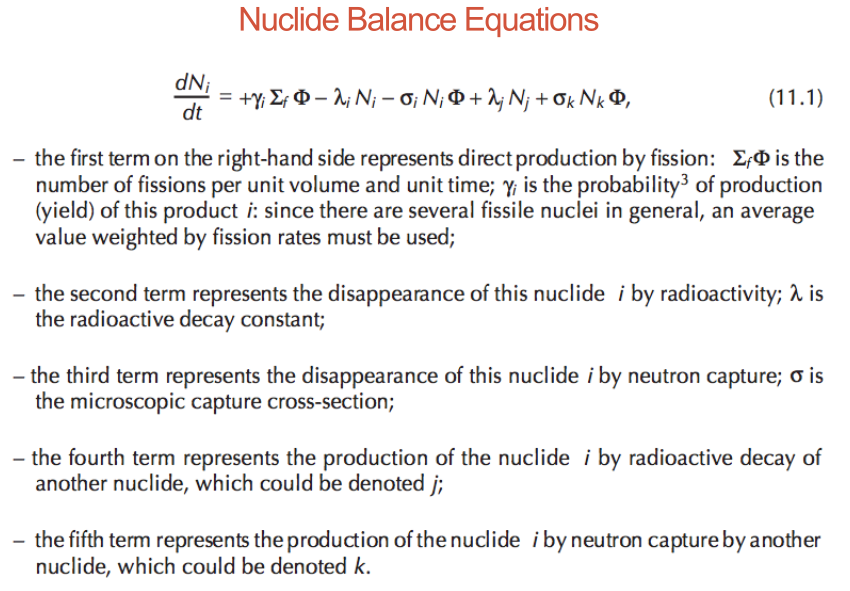
\includegraphics[width=4in]{images/dfs/nuclide-balance-equation.png}
  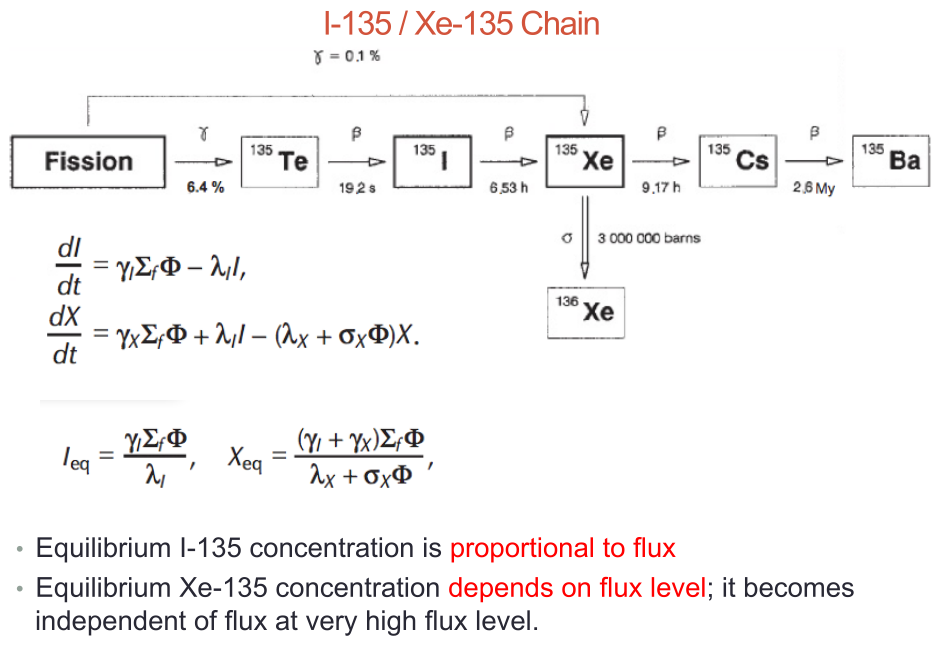
\includegraphics[width=4in]{images/dfs/I-Xe.png}
  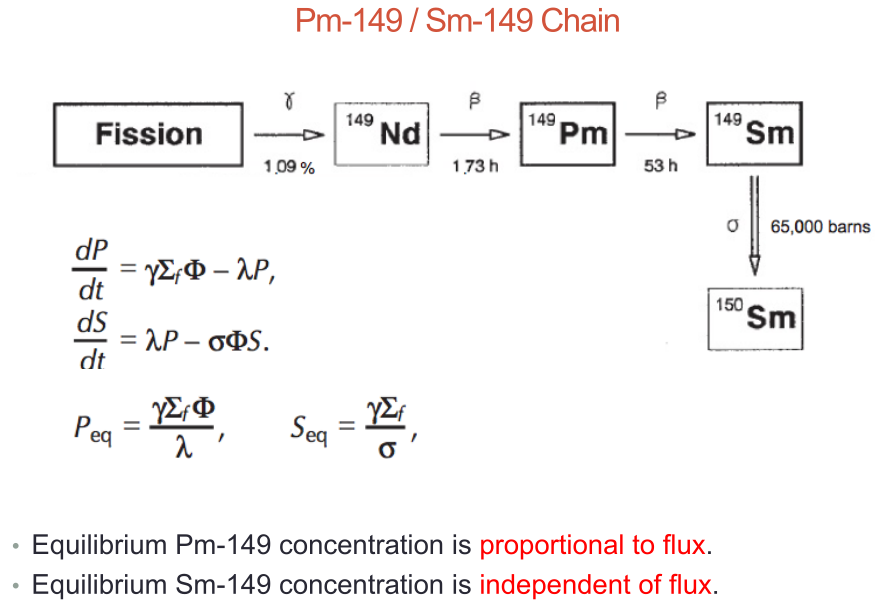
\includegraphics[width=4in]{images/dfs/Pm-Sm.png}
  \caption{Nuclide Balance Equation} \label{nbe} 
\end{figure}



\clearpage
\topic{Iodine/Xenon} \label{FP-Xenon}
Xe-135 has a thermal absorption cross section of $2.6\times 10^6$ barns. 
\begin{itemize}
\item Major source: Iodine decay; \ce{^{135} I ->^{\beta^-} ^{135}Xe} which happens with a half-life of 6.6 hours.
\item Major sink: burnup. Xe has a huge absorption xs ($10^6$ barns), so \ce{^{135} Xe + n -> ^{136} Xe}. Xe can also beta decay again with a half-life of 9.1 hours. 
\end{itemize}
Xenon peaking happens because after shutdown, the major sink is removed, but the major source remains, hence Xenon peaks until the Iodine depletes. Reactors must be designed with enough fuel to offset the effect of Xenon. At the end of core life, there may not be enough reactivity to override peak Xenon; such reactors are called `xenon-precluded.' If a scram occurs, a restart may not be possible for 30-40 hours. See Stacy's Example 6.2 (p.214) for an example of xenon reactivity worth and illustrating diagrams. 



\begin{table}
  \centering
  \begin{tabular}{|p{0.6\textwidth}|p{0.4\textwidth}|}\hline
    \begin{minipage}[b]{0.6\textwidth}
      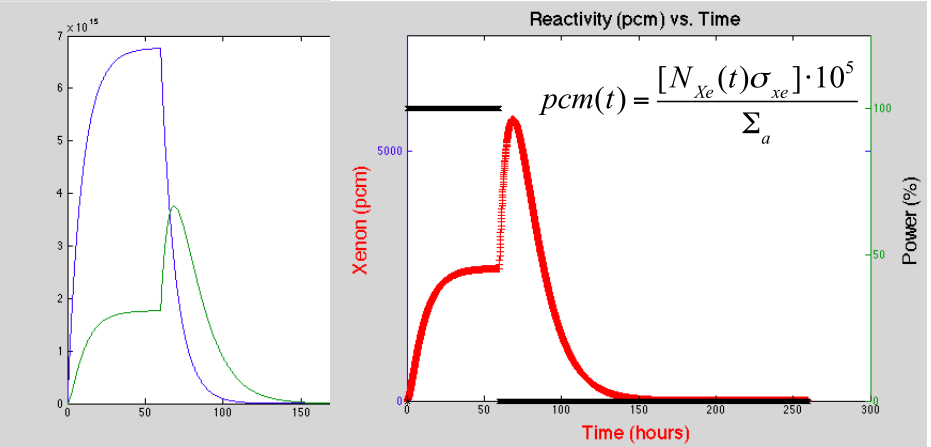
\includegraphics[width=3.5in]{images/dfs/I-Xe-1.png} 
    \end{minipage}
    & 
    \begin{minipage}[b]{0.4\textwidth}
      After startup: both I and Xe increases, and saturates after \hi{30 hrs}. After shutdown: I decays quickly, whereas Xe peaks \hi{9 hrs} after shutdown, and decays away in 60 hours. The peak happens because I coninues to decay into Xe, while Xe can no longer decrease through capture. 
There is a 2.5\% depress due to Xe; the higher the flux, the higher the peak is.
    \end{minipage}   \\ \hline
%
    \begin{minipage}[b]{0.6\textwidth}
      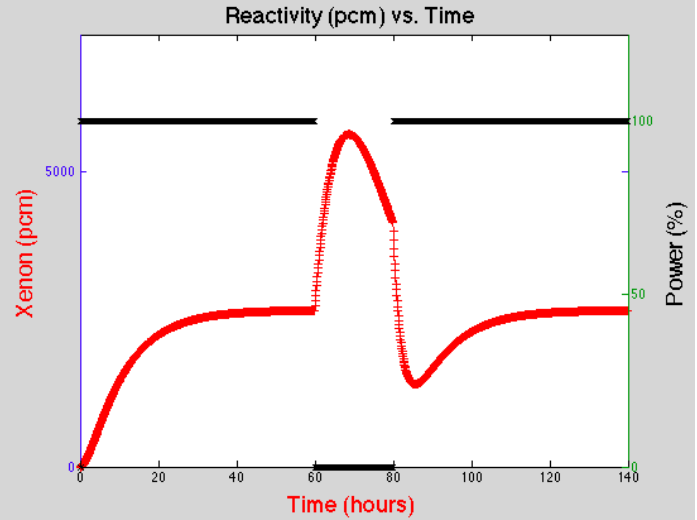
\includegraphics[width=3.5in]{images/dfs/I-Xe-2.png} 
    \end{minipage}
    & 
    \begin{minipage}[b]{0.4\textwidth}    
      A rapid startup after a scram: the concentration decreases immediately after the startup, because Xe absorption increases suddenely due to flux, which over-weights the amount from I decay. Xe would reach its equilibrium value again after about 40 hrs. 
    \end{minipage}  \\ \hline
%
    \begin{minipage}[b]{0.6\textwidth}
      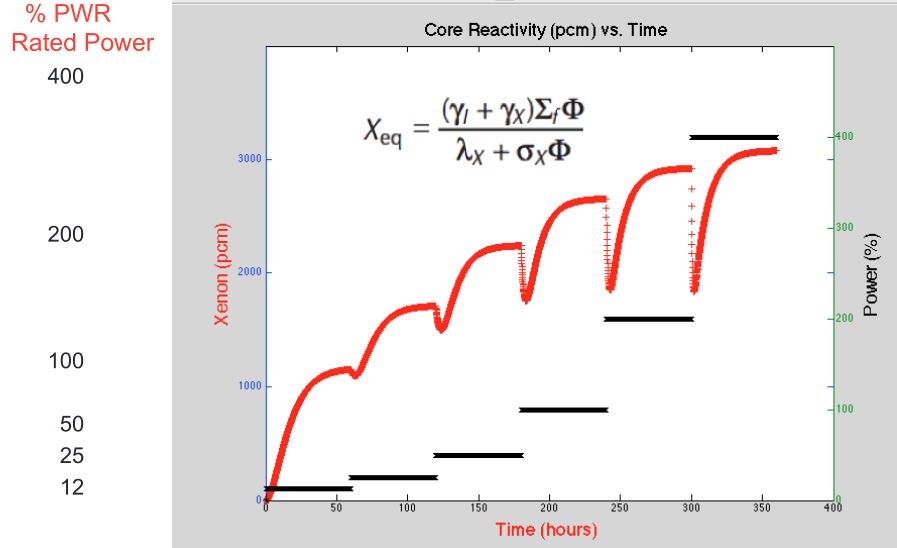
\includegraphics[width=3.5in]{images/dfs/I-Xe-3.png}
    \end{minipage}
 &  
    \begin{minipage}[b]{0.4\textwidth}    
      Equilibrium Xe Worth: if $\phi \to \infty$, then $X_{eq}$ is independent of $\phi$ as shown in the $X_{eq}$ expression; additionally, the Xenon concentration drops right after everytime power increases for the same reason as the previous case (flux increases, the destruction rate of Xe increases instantenously, but the Iodine decay rate has not increased yet). 
    \end{minipage} \\ \hline
%
    \begin{minipage}[b]{0.6\textwidth}
    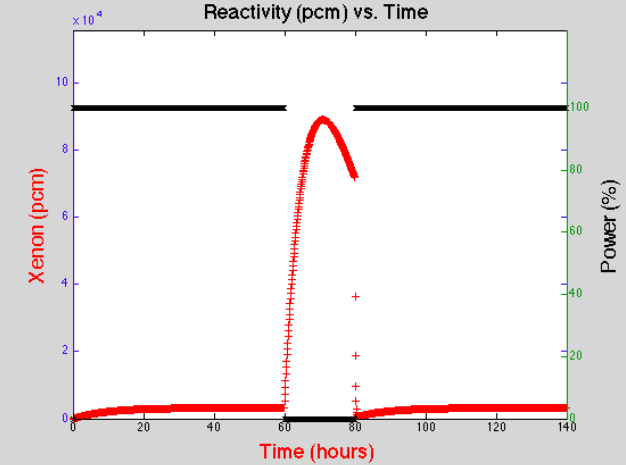
\includegraphics[width=3.5in]{images/dfs/I-Xe-4.png}
    \end{minipage}
 &  
    \begin{minipage}[b]{0.4\textwidth}
      Xe for high flux reactor: Xe peak gives rise to a control constraint. If the reactivity reserves (control rods or poisons that can be removed) are insufficient, the reactor cannot be restarted during this period of increased Xe poisoning. We have to wait till Xe drops to re-start. Alternatively, you can start before Xe builds up, which is pretty rare. 
      \end{minipage} \\ \hline
  \end{tabular}
\end{table}


\clearpage
\topic{Promethium/Samarium} \label{FP-Sm}
Samarium is another fission poisoner. It has one source: decay of Promethium; it has one sink: burnup. 

\begin{table}
  \centering
  \begin{tabular}{|p{0.6\textwidth}|p{0.4\textwidth}|}\hline
    \begin{minipage}[b]{0.6\textwidth}
      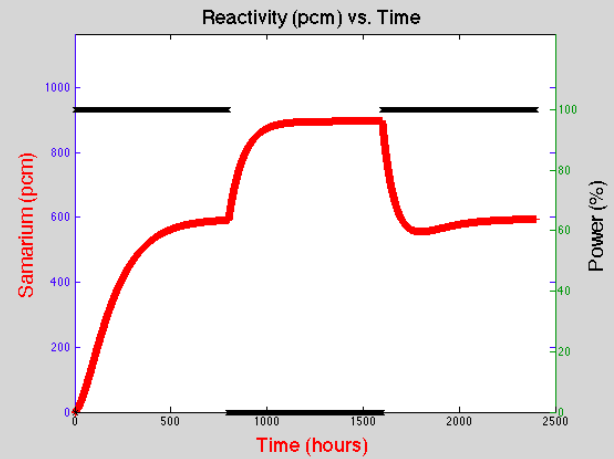
\includegraphics[width=3.5in]{images/dfs/Pm-Sm-1.png} 
    \end{minipage}
    & 
    \begin{minipage}[b]{0.4\textwidth}
      Promethium behaves normally: it builds up and reaches equilibrium when in operation, and it decays away after shutdown. 
Sm behaves similar to Xe in the sense that both peaks after reactor shutdown (Sm peaks \hi{200 hrs} after shutdown, Xe peaks 9 hrs after shutdown). But Sm is stable unlike Xe, and once Pm burns out, Sm would stay constant and never decay away. Sm reactivity peaks by 200-300 pcm after shutdown. 
    \end{minipage}   \\ \hline
%
    \begin{minipage}[b]{0.6\textwidth}
      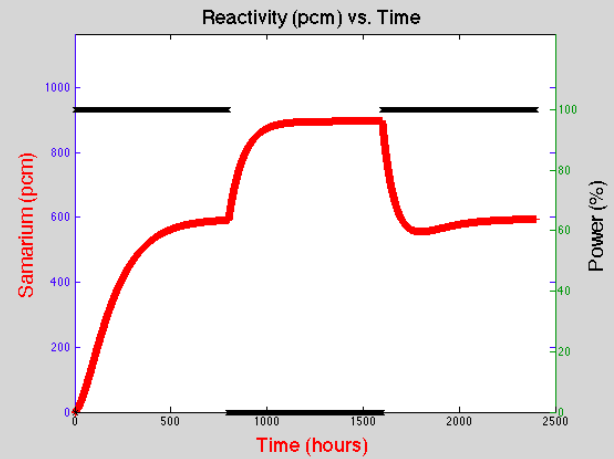
\includegraphics[width=3.5in]{images/dfs/Pm-Sm-2.png} 
    \end{minipage}
    & 
    \begin{minipage}[b]{0.4\textwidth}    
     Sm worth following a refueling outage: Over-write Xenon by pulling the control rods out for a couple of days; then insert the control rods for Sm. Sm returns to equilibrium about 100 hours after restart.
    \end{minipage}  \\ \hline
%
    \begin{minipage}[b]{0.6\textwidth}
      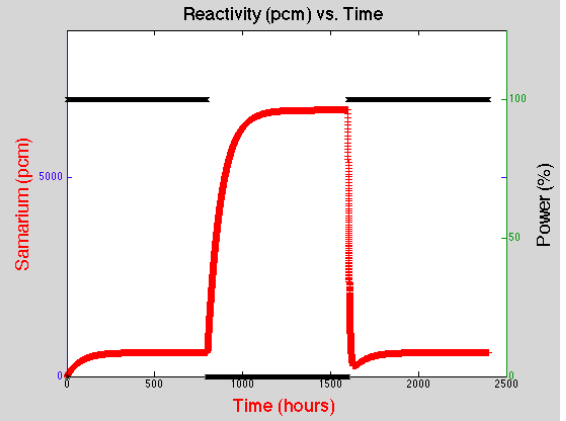
\includegraphics[width=3.5in]{images/dfs/Pm-Sm-3.png}
    \end{minipage}
    &  
    \begin{minipage}[b]{0.4\textwidth}    
      Sm for high flux reactor (20x PWR power density): Sm peaks a lot, which is bad because we may never be able to overrid Sm reactivity without refueling. Hence we should always have a controlled shutdown that burns out Xe/Sm before they build up. 
    \end{minipage} \\ \hline
  \end{tabular}
\end{table}

\clearpage
\topic{Spatial Xenon Oscillations}
When a flux tilt is introduced into a reactor, the Xe concentration will initially increase in the region whose flux is reduced, and initially decrease in the region of increased flux. This shift in the Xe distribution is such as to increase (decrease) the multiplication properties of the region in which the flux has increased (decreased), thus enhancing the flux tilt. After a few hours the increased Xe production due to the increasing I concentration in the high-flux region causes the high-flux region to have reduced multiplicative properties, and vise versa. This decreases, and may reverse, the flux tilt. In this manner it is possible under certain conditions for the delayed Xe production effects to induce growing oscillations in the spatial flux distribution\footnote{Quoted from Stacy's Section 16.6 on page 642}. 

Chasing Xenon, meaning placing the control rods where there are high concentration of Xenon, is wrong because we are nine hours out of sync then. 
\begin{figure}[ht]
  \centering
  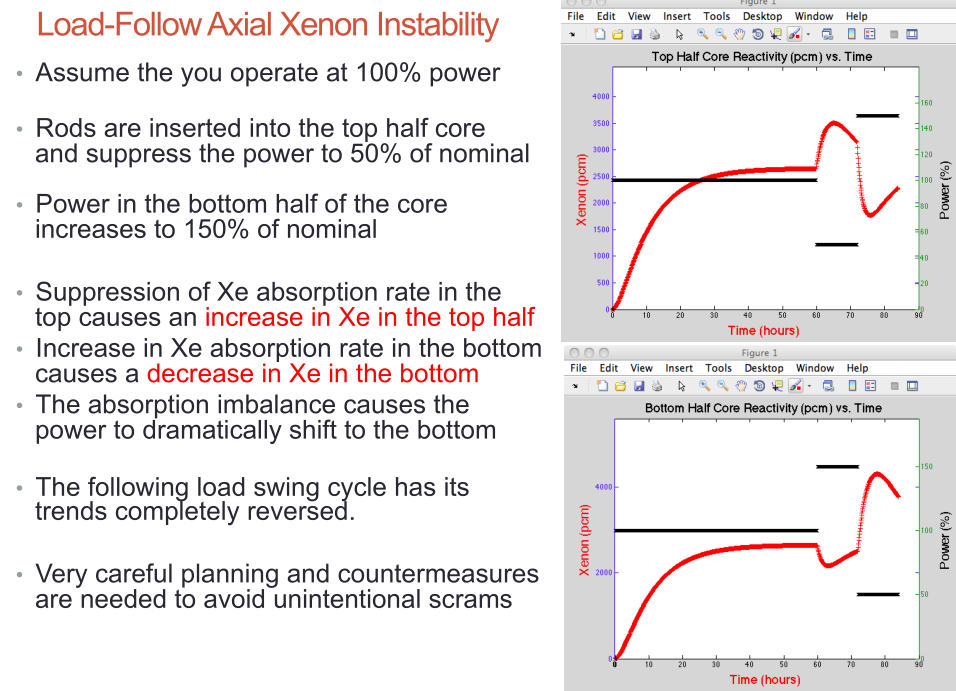
\includegraphics[width=5in]{images/dfs/axial-xenon-instability.png}
\end{figure}

\clearpage
\topic{Production Codes' Fission Product Modeling}
\begin{enumerate}
\item Point Fuel Models: ORIGEN: complete isotropic model. 
\item Lattice Physics: 
  \begin{itemize}
    \item Traditional models: 30 FPs, 2 lumped FPs (these fission products do not saturate; they increase as burnups).
    \item Latest codes: 250 FPs. 
  \end{itemize}
\item Core Models: 
  \begin{itemize}
    \item Traditionally: explicit I/Xe, Pm/Sm, all other FPs are resiual macros (depend on burnups);
    \item Latest codes: about 30 FPs, all other FPs count as residual macros vs. BU. 
  \end{itemize}
\end{enumerate}

Benchmark: Nd is a burnup marker term b/c of its low absorption cross section.   Each fission produces a fixed amount of Nd (Pu and U produces slightly different amount of Nd). Use Nd number density and the yield, you can back out the burnups. 

Gd156 and Gd157 are important for startups when using old rods (15 years old). Once operating, we don't really care about Gd that much. 


\end{document}

\documentclass{school-22.211-notes}
\date{April 11, 2012}

\begin{document}
\maketitle

\lecture{Fuel Depletion} \label{fuel-depletion}
For fuel assembly depletion, the reactivity of fuel changes dramatically with burnup. 

\topic{Actinide Chain Construction}
Normally we would model around 400 actinides; for this class, we only discuss 22 of them, which occupies the high-end of actinides (with large N, large Z). 

What happens during actinide chain construction? 
\begin{enumerate}
\item Fission product absorptions reduce reactivitiy of the fuel significantly, often 10-20\%;
\item \ce{^{235}U} depletion significantly ...

\item Fission cross section: isotopes have threshold energies, producing step-shape near higher energies (around 10 MeV)\footnote{Both even and odd isotopes have threshold energies, but odd isotopes have higher resonance fission cross section, hence even isotopes' threshold energy behavior is more pronoud.}. Remember Pu is very fissile material. Am242 is a funny one -- although it's an even isotope, its fission cross section is large. 

\item Simple actinide nuclide transmutation model. In Figure, the red arrors designate the actinide chains we model (chains end at isotopes that decay quickly compared with the phenomena we are trying to model); blue arrors designate beta decay. 

\item The higher you go up the chain (e.g., into the MA region), the worse the absorption would be. 

\item Branching ratio is a function of energy. Example: \ce{^{241}Am} can produce \ce{^{242}Am} with a half-life of 16 hrs, and the meta-stable \ce{^{242m}Am} with a half-life of 141 years. \ce{^{242}Am}'s thermal branching ratio is about 10\% that of \ce{^{242m}Am}. 
\end{enumerate}


\clearpage
\topic{Actinide Chain Solutions}
Recall our nuclide balance equation. For this model, we do not have the `direct production by fission' term anymore.  No fission yield term. 

Compare fission product matrix form vs. actinides matrix formin Fig.~\ref{fp-an-matrix-form} : 
\begin{figure}[ht]
  \centering
  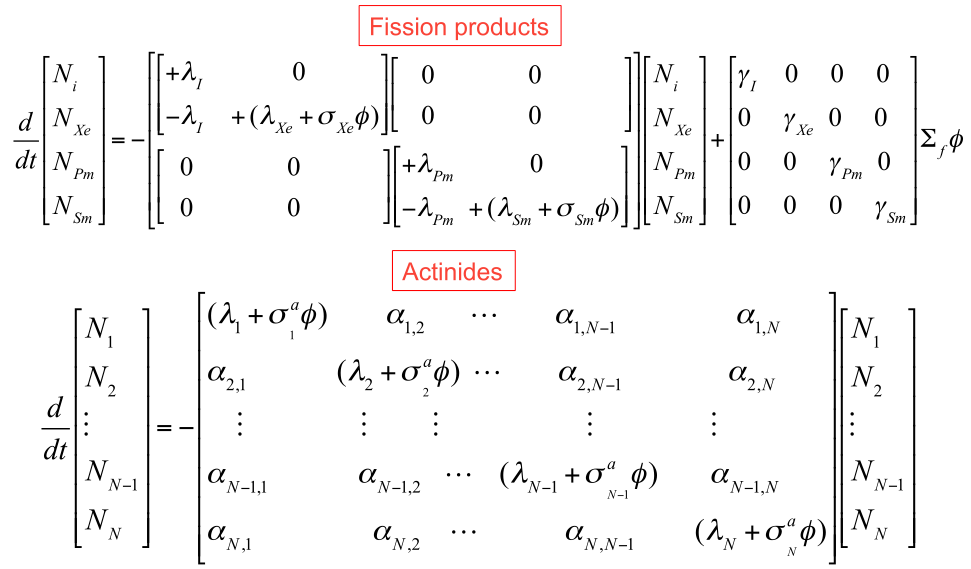
\includegraphics[width=5in]{images/dfs/fp-an-matrix-form.png}
  \caption{Nuclide Depletion Equations vs. Actinide in Matrix Form} \label{fp-an-matrix-form}
\end{figure}
\begin{itemize}
\item Actinides matrix form has no fission yield term;
\item Fission product matrix is decoupled; actinide matrix is not; 
\end{itemize}


More specifically, we focus on the actinides matrix, and notice: blue circles are decay coupling term; a n2n reaction with isotope 2 produces isotopes 1. 

\begin{figure}[ht]
  \centering
  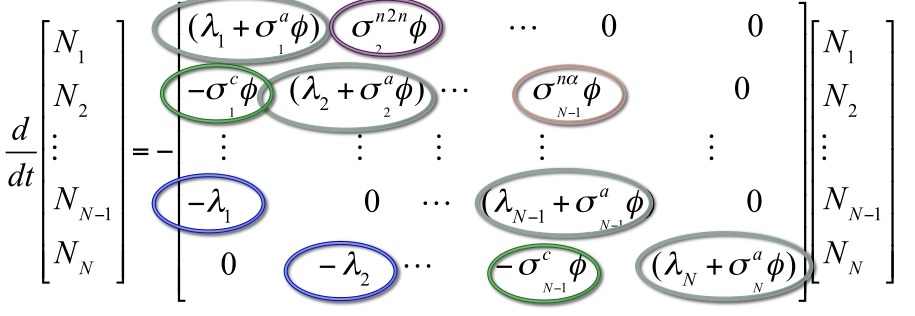
\includegraphics[width=5in]{images/dfs/nuclide-depletion-matrix-form.png}
  \caption{Nuclide Depletion Equations vs. Actinide in Matrix Form} \label{nuclide-depletion-matrix} 
    \end{figure}


There are 4 blocks for the 4 species as in Fig.~\ref{actinide-block}. 
\begin{figure}[ht]
  \centering
  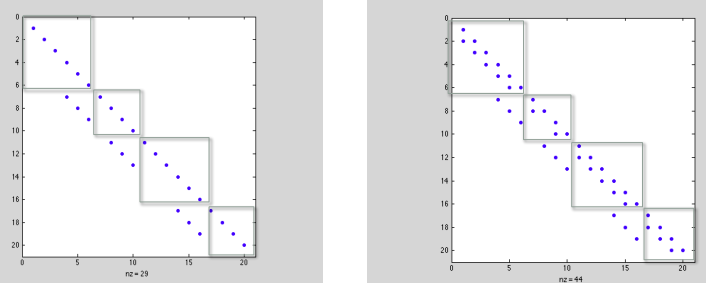
\includegraphics[width=5in]{images/dfs/actinide-block.png}
  \caption{Matrix Shape for Actinide Depletion Equations} \label{actinide-block} 
    \end{figure}
\begin{itemize}
\item The decay terms sit outside of the blocks; they couple the blocks.
\item  The capture terms are one line off the diagonal term (NP238 decays so quickly that its capture cross section is zero and is not shown throug the spy function in matlab); 
\item We don't have above the diagonal term because we ignore the $n2n$ reaction and the $n \alpha$ reaction. The reason we ignore them is that having a sub-diagonal matrix we can invert analytically; whereas having a full matrix is a lot harder to invert. Another simplification we made is to ignore all meta-stable states and only have the ground states, hence ignoring branching. 
\end{itemize}

\textbf{Understanding the solutions we obtained}:
\begin{enumerate}
\item U238 barely changes; there are a lot of it, and it probably decreases by 1\%; often time the nuclear concentration is plotted with respect to initial heavy metal inventory, that is, U238 concentration. 
\item U234, U235 does not have production, hence it decreases. 
\item U236 is produced as we burnup U235; U236 has almost no destruction rates;
\item U237 is produced as we burnup 
\item U239 is a constant because its capture from U238 is constant, and U239 decays so quickly (23 mins) that it's at equilibrium the whole time. 
\item (remember) Np has a half-life of 2 and 2.5 days; Np's cancels out Am etc, and they have the same half-life, so people use to ignore them. 
\item Production with Pu; 
\item Am244: takes a certain burnup to come up. Even though Am is a small concentration, we still care about them. 
\end{enumerate}

About 40-50\% of power would be produced from Pu instead of U by the time we shut down the reactor. 





\clearpage
\topic{Burnup Units}
\begin{enumerate}
\item FIFA = fission per initial fissile atoms;
\item FIMA = fission per initial (heavy) metal atoms;
\item Atom percent (A\%) = FIMA * 100;
\item Burnup: GWd/T = MWd/kg = thermal power per weight of heavy metal. 
  \begin{itemize}
    \item Advantages: we know the reactor power and 
    \item Disadvantages: `energy released' is not a very clean term; we don't really care about neutrino energy, gamma energy released from capture of neutrons; energy deposited in fuel assembly B from fissions in assembly A. In LWR, it is a good approximation to assume that energy is depositied where the fission is; in MITR it is a bad approximation, fission product energy (deposite locally), gamma heat energy (not necessarily deposited locally), etc. 
  \end{itemize}
\item EFPHs = Effective Full Power Hours; EFPD = Effective Full Power Days. 
\end{enumerate}

\clearpage
\topic{Numerous Subtle Effects}
\begin{enumerate}
 \item We didn't really cover the Thorium/U233 Chain in Kord's class. 
   \begin{itemize}
   \item The chain for Th is very complicated; there are n2n reactions at all different levels; there are multiple ways to get U232; 
   \item some of these isotopes have very rapid alpha decays; 
   \item Pa233 has 27 day half-life; 
   \item U232 has 70 year half-life; U232's daughter product Ta208 has 2.6 MeV gamma (which is the hardest gamma known). 
   \end{itemize}
   Coverage of Th/U233 comparison from Ben's class (11/29). [FIXME]


\item Burnable Poisons History Effect: hardern the spectrum, because it pushes some water away, BP history effect: you place BP in it at the beginning of the reactor, we take it out later hence to achieve flat power through time. The BP effect is about 250 pcm. 

\item Fuel Temperature Depletion History Effects: 
Initially, the instantenous temperature effect is almost independent of depletion; as the burnup increases, something happens. The moral of the story is, we not only need to know the burnup but also the temperature. 

\item Gadolinium burnable absorber: 
  \begin{itemize}
  \item Gadolinium has a huge thermal absorption cross section. It's almost as high as Zn, but we cannot use Zinon because it would ecay; 
  \item What we do with Gadolinium is to replace part of the fuel with Gad and reactivity would be flatter with respect to time. 
  \item Hold-down is the difference between the reactivity at the beginning of life-cycle. 
  \item Gad resdual: there is a little bit loss of reactivity due to Gad. Gad depletes from outside to inside. 
  \end{itemize}


\item Where do reaction rates come from? 
  \begin{itemize}
  \item ORIGEN uses point depletion, 
  \item Fuel pin radial shape: the outter region almost have 2 times the flux compared with the inner ones. 
  \end{itemize}

\item Benchmark: 
  \begin{itemize}
  \item data set is the single most important things in determine the accuracy of your codes.
  \item U235 has a pretty large error, but we don't care because there is so little of it;
  \item Accuracy tends to decrease the further up the decay chains. 
  \item Measurements also have an intrinsic uncertainty; do not rely on single measurement campaigns; systematic errors in measurements are common. 
  \item In performing `actinide burner' analysis, when we place the actinide at the end of one analysis into another one, the error builds up. 
  \end{itemize}
\end{enumerate} 



\clearpage
\topic{Spent Fuel and Recycling}
[FIXME] 11/29/12. 

\begin{enumerate}

\item Pu enrichment is higher than U enrichment for two reasons: a) only 60\% Pu is fissile \ce{^{239}Pu}, the rest of them are parisitic; b) Pu has a higher absorption rates. 

\item The majority of the spent fuel is U238 which is not real waste; the U and Pu in the spent fuel is sent back to the core. The real waste is limited to MA and is vitrified in a borosilicate glass form. 

\item Multi-recycling: we cannot recycle too many times. Reason: after 1st cycle the fissile content is 64.8\%, after 2nd cycle fissile is only 51.1\% and requires a higher Pu enrichment; and if Pu enrichment is pass xxx, then the void coefficient would become positive. 

\item DUPIC cycle (used in CANDU): it is an entirely mechanical process during which we grind up everything, the gas comes out, and re-construct the grinds into fuel which contains about 0.8\% U235 and 0.8\% Pu239, which is about twice the excess reactivity of natural uranium and is more than enough for a CANDU.

\item Fast reactor transmutation: at high energy, all MA are fissible (also high absorption cross section which is why we don't expect to get energy from MA), so we can transmutate MA.  


\item Th cycle advantages: 
\begin{enumerate}
\item Abundancy is 4x that of U. 
\item Less waste:  we start further bottom left from the chain, and Th cycle would generate less MA waste. 

\end{enumerate}
Companies that considers Th cycle: Thorium Power Inc which is a subsidiary of Lightbridge Corp. 
\end{enumerate}


\end{document}

\documentclass{school-22.211-notes}
\date{April 25, 2012}

\begin{document}
\maketitle

\lecture{Point Kinetics Without Feedback}
\topic{Physics of Delayed Neutrons}
\textbf{Prompt neutrons}: more than 99\% of all neutrons are emitted within $10^{-10}$ seconds after the fission. Prompt neutron lifetime in a PWR is about $2 \times 10^{-5}$s. Example: A reactor was operated at 1W, a control rod was moved to produce an excess reactivity of $0.0005 \Delta k$, what would the power be 1s later? 
\begin{align}
P(t) &= P_0 (1.0005)^{t/(2\times 10^{-5})} = 1 W (1.0005)^{1/(2\times 10^{-5})} = 70,000 MW 
\end{align}
The above calculation means that this reactor would be virtually impossible to control! Fortunately, delayed netrons exist and the reactor time constant depend on more than just prompt neutron lifetime. 

\textbf{Delayed neutrons}:
\begin{enumerate}
\item Measurement: delayed neutrons can be measured by counting neutrons emission after a pulsed irradiation of a pure U235 foil. Burst measurement represents the amount of prompt neutrons; saturated measurement represents the total amount of neutrons. 
\item Emission: delayed neutrons are emitted through the decay of fission products, of which Br-37 is a dominant FP that emits delayed neutrons. 
\item Delayed yields depend on fissioning species and neutron energy (keep in mind that U238 produce 4\% delayed neutron per fission, more than U235, making U238 a very important isotope when it comes to delayed neutrons). 
  \begin{itemize}
  \item Absolute yield: number of delayed neutrons per fission; 
  \item Relative yield: percentage: absolute yield of this isotope divided by total absolute yield; 
  \item Delayed neutron fraction: absolute yield divided by nu bar.  
  \end{itemize}
\item Modern trend: makes the 6-group to 8-group, and each group has a fixed decay constants (the one that dominants in the group, that is, largest half-life). This way, all isotopes have the same half-life for the same group; but different isotopes would still have different delayed neutron fraction. Remember the terms circled in blue.  
\item Delayed neutrons spectrum: average prompt neutron emission energy is 2MeV; average delayed neutron emission energy is 0.4MeV. Both spectrum comes out to be Maxwellian, except the delayed one is shifted. Delayed neutron comes out in the thermal energy range, which makes them more likely to fission. Delayed neutron spectra vary only slightly for different fissioning nuclides; but the spectra depends significantly on the delayed neutron group. 
\end{enumerate}

\clearpage
\topic{Derivation of Point Kinetics Equations (PKE)}
In steady-state transport or diffusion equation, we do not treat delayed neutrons directly. But the fission emission spectrum must be properly weighted with prompt and delayed contributions. Notice one issue is, we need fission rates to get $\chi$, and we need $\chi$ to get fission rates, so the real way to solve the balance equation is to iterate, though this is not how it is done normally.
\begin{enumerate}
\item We start from the diffusion equation: \hi{The steady-state diffusion equation}\footnote{Know this for the final}: 
\begin{align}
& - \divergence D(\vecr, E, t) \gradient \phi(\vecr, E, t) + \Sigma_t (\vecr, E, t) \phi(\vecr, E, t) = \int_0^{\infty} \Sigma_s (\vecr, E'\to E, t) \phi(\vecr, E', t) \dE' \\
&+ \Sum_j \chi_T^j (E) \int_0^{\infty} \nu \Sigma_p^j (\vecr, E', t) \phi(\vecr, E', t) \dE' + Q(\vecr, E, t) 
\end{align}

\item \hi{The time-dependent neutron diffusion equation}: where $\beta^j = \Sum_i \beta_i^j$ is the delayed fission fraction (0.66\% for instance), 
\begin{align}
\ppt \left[ \frac{1}{v} \phi(\vecr, E, t) \right] &= \divergence D(\vecr, E, t) \gradient \phi(\vecr, E, t) - \Sigma_t (\vecr, E, t) \phi(\vecr, E, t) \\
& + \int_0^{\infty} \Sigma_s (\vecr, E'\to E, t) \phi(\vecr, E', t) \dE' \\
&+ \Sum_j \chi_p^j (E) (1-\beta^j) \int_0^{\infty} \nu \Sigma_p^j (\vecr, E', t) \phi(\vecr, E', t) \dE' \\
&+ \Sum_i \chi_d^i (E) \lambda_i C_i (\vecr, t) + Q(\vecr, E, t)\\
\ppt C_i (\vecr, t) &= \Sum_j \beta_i^j \int_0^{\infty} \nu \Sigma_p^j (\vecr, E', t) \phi(\vecr, E', t) \dE' - \lambda_i C_i (\vecr, t) 
\end{align}

\item Assume that flux can be separated into a space/energy term and a time-dependent term: $\phi(\vecr, E, t) = S(\vecr, E) T(t)$. Then we can manipulate the time-dependent neutron diffusion equation, 
\begin{align}
\ppt \left[ \frac{1}{v} S(\vecr, E) T(t) \right] &= \divergence D(\vecr, E, t) \gradient \phi(\vecr, E, t) - \Sigma_t (\vecr, E, t) \phi(\vecr, E, t) \\
& + \int_0^{\infty} \Sigma_s (\vecr, E'\to E, t) \phi(\vecr, E', t) \dE' \\
&+ \Sum_j \chi_p^j (E) (1-\beta^j) \int_0^{\infty} \nu \Sigma_p^j (\vecr, E', t) \phi(\vecr, E', t) \dE' \\
&+ \Sum_i \chi_d^i (E) \lambda_i C_i (\vecr, t) + Q(\vecr, E, t)\\
\ppt C_i (\vecr, t) &= \Sum_j \beta_i^j \int_0^{\infty} \nu \Sigma_p^j (\vecr, E', t) \phi(\vecr, E', t) \dE' - \lambda_i C_i (\vecr, t) 
\end{align}

\item top of rho: diffusion equation, if steady state, top is zero. 
bottom of rho: fission rate (if all the neutrons show up instatenously, the bottom would be the fission rate). 

Gamma = 1/v of shape divided by almost-instantenous-fission-rate. 

\end{enumerate}

\clearpage
\topic{Simple Matlab Methods for Solving PKEs}

\begin{enumerate}
\item Instantaneous reactor scram ($\rho = - 8 \beta$): 

Question: does the 8 group happen to have half-lives from large to small? 
\item Two seconds rod drop ($\rho = - 8 \beta$):

\item Instantaneous rod withdraw ($\rho = 0.1 \beta$): 
The reactor wants to response immediately (hence it jumps) but it does not have enough delayed neutron to sustain that increase, hence the jump is not enough and it will increase for the rest of the way. To estimate the prompt jump, we do the prompt jump approximation (easy to do in 1 group)

\item 4b: if we wait long enough, we reach secular equilibrium between power and precursor rate that the precursor rates have the same shapes as the power, altough the rates may be off by a factor. 

\item 

\item Power does not come back to the same level, because we are solving for an eigenvalue problem, and what the asymptotic power is depends on how to get there. In the withdrawal case, the precursor builds up and is continuing to build up during the second phase, so the power ends up higher than initially. 


\item Super-prompt criticality: when reactivity exceeds beta, reactivity does not have to wait for the delayed neutrons anymore, changes can happen instantaneously.  
\end{enumerate}



\clearpage
\topic{Understanding Reactor Behavior with PKEs}
\subtopic{Negative Reactivity Excursions}


\subtopic{Positive Reactivity Excursions}


\subtopic{Prompt Excursions}

\clearpage
\topic{Approximate Solutions}
\subtopic{Prompt-Jump Approximations}


\subtopic{In-hour Equations: THe Simpliest Inverse Kinetics Application}
From the PKEs, know how to derive the In-hour Equation: 
\begin{align}
\Aboxed{ \rho &= \omega \Lambda + \Sum_i \frac{\beta_i \omega}{\omega + \lambda_i}}
\end{align}
That is, knowing every other term, we can back out reactivity $\rho$ assuming there is no feedback. The steps are: 


\clearpage
\topic{Reactivity Units}
\begin{table}[ht]
  \centering
  \begin{tabular}{|c|c|c|}
    $\Delta k$ & actual units of PKEs & 0.01 \\
    \% $\Delta k$ & & 1/% \\
  \end{tabular}
\end{table}

\clearpage
\topic{Derivation of Inverse Kinetics Equations (IK)}
Assume we know the amplitude function $T(t)$, we can solve for the pre-cursor function $C(t)$; then plugging back in the PKEs, we can get $\rho(t)$. 



\clearpage
\topic{Experimental Applications of IK}
\subtopic{PWR Boration/Dilution}

The red curve is measured by detectors. Prompt neutron life time is so short, so that even spatial distribution flux changes a lot, we can assume that it stabalizes already at each rod drop. 

Disadvantages: time concern; boration dilution increases cost with waste disposal.  

Alternatives: we use General Inverse Kinetics to get around about it. 

\subtopic{SCRAM/Rod Drop Analysis}
From scram, we measure power change, infer $T(t)$, and estimate reactivity.

The rough method use Prompt Jumpt Approximation,


More accurately, we need to model all the neutron sources, including ($\alpha,n$) reactions etc. It comes out to be, 


In reality, there are noisy signals in measured power and reactivity data; we need to smooth them out with a fitted function before we can apply IK with external neutron sources. 

This technique is not used in the US that much because it is harsh your system and it requires work to bring the system back to critical. But it is one of the best ways to demonstrate to the licensing committee that a reactor is capable to scram.  

\subtopic{Dynamic Rod Worth}
We start with a critical reactor, and drive a control rod in and out and repeat with a different rod. The advantages are: no need to do boron dilution, and it takes 15 mins for each rod. This technique is widely used by Westinghouse to estimate their rod worth. 




Alternatively, we can do sub-critical source multiplication, that is, IK with a source in the reactor. This way we don't even need to start with a critical reactor. This technique has only been used in experimental reactors but not so much in power reactors because it requires detailed knowledge about the source distribution. 

\subtopic{Oscillator Sample Worth Measurements}


\clearpage
\topic{Summary}
Shape function $S(\vecr, E)$, amplitude function, $T(t)$. 

PKT: the top of $\rho$ is just the steady-state diffusion equation; at steady state, $\keff = 1, \rho = 0$. 

There are four fundamental thing: diffusion equation, point-kinetics equation, derive the prompt-jump approximation, derive the in-hour equation. 


Questions:  p.12, steps. 
p.19, why don't image 1 match image 4: because step sizes are not uniform. 
p.27, 
p.29

\end{document}

\documentclass{school-22.211-notes}
\date{April 30, 2012}

\begin{document}
\maketitle

\lecture{Point Kinetics With Feedbacks}
Why we care about feedbacks? 
\begin{enumerate}
\item In a RIA safety analysis, if we perform a rod ejection at hot zero power, the local flux distribution changes. Also the magnitude of flux/power can change from a few Watt to 20,000 MW in less than 1s! 

\item It used to be we model all fuel fresh and assume an artificially high rod worth. Then people realize that the fuel enthalpy at failure is dependent on fuel BU (the higher the BU, the easier it is for the fuel to fail) as in Fig.~\ref{failure-depend-on-BU}. Thus we need to model control rods somewhat faithfully to get a reasonable safety analysis. 

  \begin{figure}[ht]
    \centering
    \includegraphics[width=4in}{images/pke/failure-depend-on-BU.png}
    \caption{Fuel Enthalpy at Failure Depends on Fuel BU} \label{failure-depend-on-BU}
  \end{figure}


\item The importance of modeling feedback can be illustrated in Fig.~\ref{feedback}. Without feedback, the reactor wants to be a bomb and the power would shoot up. With Doppler feedback, both the reactivity and the power would damp down. If correctly designed, reactors would use feedback effects to keep them from acting like bombs\footnote{There is no Doppler feedback for fast reactors, so fast reactors have to do all kind of tricks to get a negative feedback. Also fast reactors have positive sodium void worth, because as energy deposits in the sodium, voids are generated, pushing sodium away, generating a positive sodium void worth}. 
\end{enumerate} 
  \begin{figure}[ht]
    \centering
    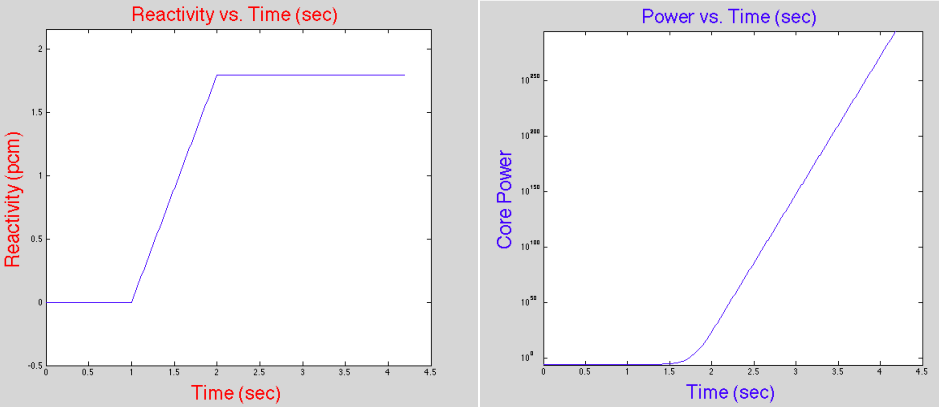
\includegraphics[width=4in]{images/pke/feedback1.png}
    \\
    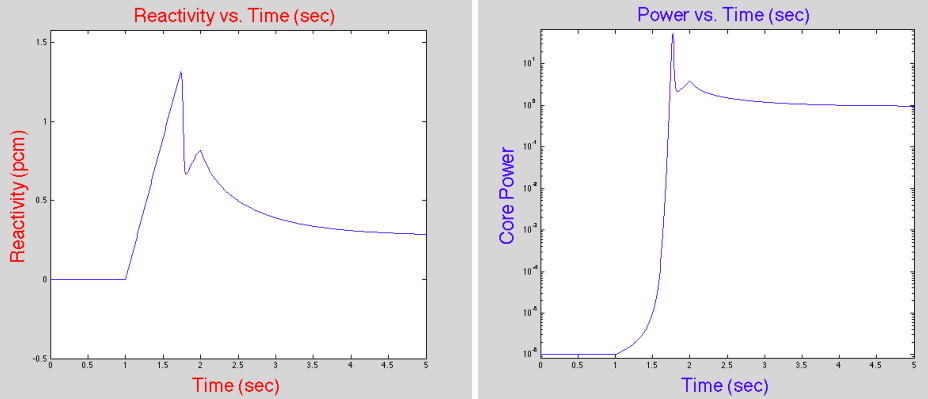
\includegraphics[width=4in]{images/pke/feedback2.png}
    \caption{\$1.5 RIA With or Without Doppler Feedback}\label{feedback}
  \end{figure}



\clearpage
\topic{Fuchs-Nordheim Model}
The Fuchs-Nordheim Model predicts the shape and the magnitude of the transient. We do not really solve the analytical solution of this model, but instead study some characteristics from it. 

\subtopic{Assumptions}
To start, we make three assumptions\footnote{The historical reason for these assumptions is that the model was developed for weapon use, hence $\rho \gg \beta$ and rapid transient.}, 
\begin{enumerate}
\item If $\rho \gg \beta$, we can ignore the delayed neutrons and hence write the power distribution $P(t)$ as the 1st equation in PKE (we use $P(t)$ instead of $T(t)$ for the shape function now to avoid the confusion with temperature $T$ that we would use repeatively in this section). 
  \eqn{ \ddt P(t) &= \frac{\rho(t) - \beta}{\Lambda} P(t) + \Sum_i \lambda_i C_i (t) \approx \frac{\rho(t) - \beta}{\Lambda} P(t) \label{fn-eq1}}
  It is fair to ignore the precursors, because as in Fig.~\ref{fn1} top row, we can see that the power with precursor is small enough that the F-N model provides good approximation. The bottom row of Fig.~\ref{fn1} is plotted on a log-log scale to show the small difference made by the precursors.  
\begin{figure}[ht]
  \centering
  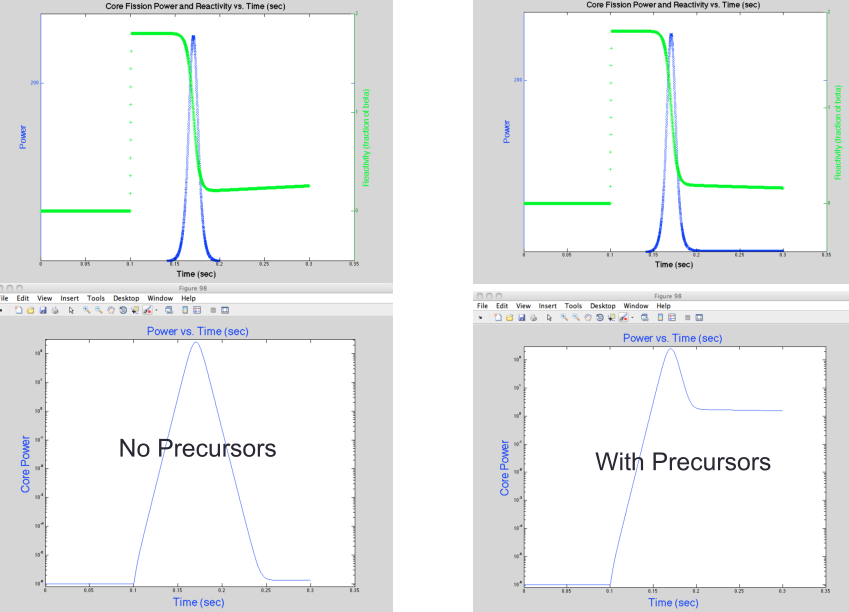
\includegraphics[width=6in]{images/pke/fn1.png}
  \caption{Assumption in Fuchs-Nordheim: No Precursors}\label{fn1}
\end{figure}

\item If transient is so rapid that no heat transferred form the fuel \footnote{The time constant for heat to be removed from \ce{UO_2} fuel is about 5 mins.}, 
  \eqn{ T_{fuel} = T_{fuel}^0 + \frac{1}{C_p} \int P(t) \dt \label{fn-eq2} }

\item Assume a Doppler Feedback coefficient independent of temperature (recall that the doppler we calculated is about 3 pcm), 
  \eqn{ \rho(t) = \rho_{rod} - \alpha (T_{fuel} - T_{fuel}^0) \label{fn-eq3} }
\end{enumerate}

\subtopic{First Derivation}
Then we solve a first order ODE. We differentiate Eq.~\ref{fn-eq2} to get,
\eqn{ \frac{\dT_{fuel} (t)}{\dt} = \frac{P(t)}{C_p} \label{fn-eq4}}
Plug Eq.~\ref{fn-eq3} into Eq.~\ref{fn-eq1} (omit $T_{fuel}^0$), 
\eqn{ \frac{\dP(t)}{\dt} = \frac{\rho_{rod} - \alpha T_{fuel} - \beta}{\Lambda} P(t) \label{fn-eq5} }
Eq.~\ref{fn-eq5} divided by \ref{fn-eq4}, 
\begin{align}
\frac{\dP(t)}{\dT_{fuel}} &= \frac{\frac{\dP(t)}{\dt}}{\frac{\dT_{fuel} (t)}{\dt}} =  \frac{(\rho_{rod} - \alpha T_{fuel} - \beta ) C_p}{\Lambda} \\
&= \frac{1}{\Lambda} \left[ C_p (\rho_{rod} - \beta) - \alpha C_p T_{fuel} (t) \right] \\
\Aboxed{ P(t) &= P_0 + \frac{1}{\Lambda} \left[ C_p (\rho_{rod} - \beta) T_{fuel} (t)  - \frac{\alpha C_p}{2} T^2_{fuel} (t) \right]  } \label{fn-power}
\end{align}
Eq.~\ref{fn-power} can be used to find peak power behavior. For peak power, we set $\frac{\dP}{dT_{fuel}} = 0$, thus, 
\begin{align}
0 &= \frac{1}{\Lambda} \left[ C_p (\rho_{rod} - \beta) - C_p \alpha T_{fuel}^{peak} \right] \\
\Aboxed{ T_{fuel}^{peak} &= \frac{\rho_{rod} - \beta}{\alpha} } \label{fn-11} \\
\Aboxed{ P^{peak} &= P_0 + \frac{C_p (\rho_{rod} - \beta)^2}{2 \Lambda \alpha} }
\end{align}
Take-away: 
\begin{enumerate}
\item \hi{Peak temperature is independent of neutron lifetime and heat capacity.} 
\item Peak power is proportional to $C_p$, and inversely proportional to $\Lambda$. That is, fast reactors with small $\Lambda$ are going to generate a lot of heat in a short amount of time. 
\item Also notice that all of these models are derived with at least $\rho > \beta$. As $\rho \to \beta$, the above equations become very sensitive.
\end{enumerate}


\subtopic{Second Derivation}
Alternatively, we use $\frac{\dP}{\dt}$ expression from the PKEs, and $\frac{\drho}{\dt}$ expression from Eq.~\ref{fn-power} that we derived, 
\begin{align}
\frac{\dP(t)}{\dt} &= \frac{\dP(t)}{\drho} \frac{\drho}{\dt}  \\
\frac{\dP(t)}{\drho} &= \frac{  \frac{\dP(t)}{\dt} }{  \frac{\drho}{\dt} } \\
&= \frac{ \frac{\rho(t) - \beta}{\Lambda} P(t) }{ - \frac{\alpha}{\Lambda C_p } P(t)} \\
&= - \frac{C_p}{\alpha} \left[ \rho(t) - \beta \right] 
\end{align}
We integrate with repsect to $\rho$ and evaluate the constant of integration by using the step reactivity $\rho_{rod}$, 
\eqn{ P(t) = P_0 + \frac{C_p}{2\alpha} \left[ - (\rho(t) - \beta)^2 + (\rho_{rod} - \beta)^2 \right]  }
If we consider the transient terminated when $P(t)$ returns to $P_0$, then 
\eqn{ \rho_{end} = 2 \beta - \rho_{rod} }
Using the constant fuel temperature feedback coefficient, 
\eqn{ 2 \beta - \rho_{rod}  = \rho_{rod} - \alpha (T_{fuel}^{end} - T_{fuel}^0 ) }
That is, 
\eqn{ \Aboxed{ T_{fuel}^{end} &= \frac{2 (\rho_{rod} - \beta)}{\alpha} + T_{fuel}^0 } }
  Compare $T_{fuel}^{end}$ in the above expression with $T_{fuel}^{peak}$ in Eq.~\ref{fn-11}, \textbf{the final temperature is twice the temperature rise at the time of the peak power,} and it is independent of neutron lifetime and heat capacity again. 


\clearpage
\topic{Fuchs-Nordheim Examples}
\begin{enumerate}
\item \hi{Asymptotic fuel temperature is independent of the reactivity insertion rate} as in Fig.~\ref{fn2}. The power vs. time shape changes as we alter reactivity insertion rate. For instance, for 2s, there is a second peak that happens when the rod is fully inserted.  F-N model provides pretty good estimation, because temperature is basically integrated power, and the reactivity insertion rate does not matter that much because we are integrating over time. Another way to think about is that there has to be something to balance out the reactivity change, and it is the Doppler feedback, thus temperature that balance out the reactivity change. Thus the asymptotic temperature only depends on the asymptotic reactivity. 

  \begin{figure}[ht] 
    \centering
    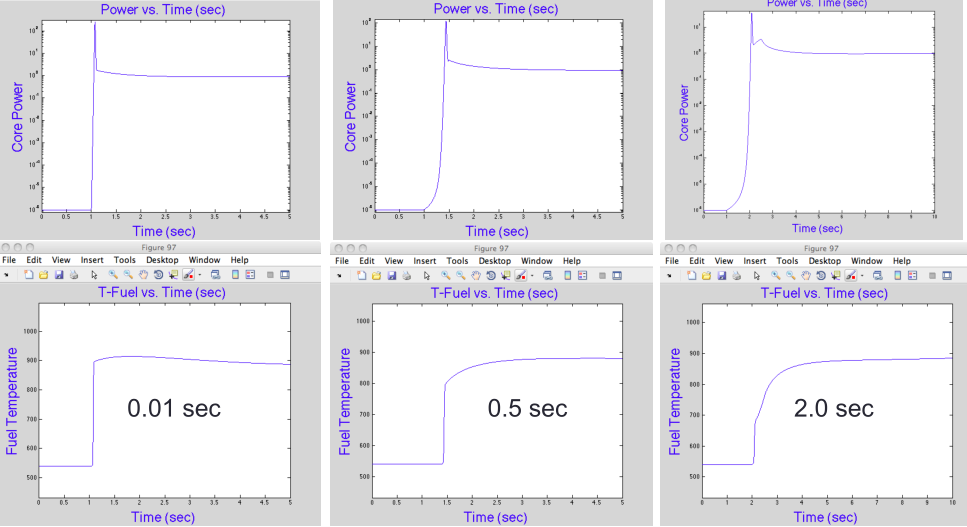
\includegraphics[width=7in]{images/pke/fn2.png}
    \caption{Fuel Temperature Independent Reactivity Insertion Rate} \label{fn2}
  \end{figure}

\item \$1.8 Insertion at Full Power: RIA at full power results in much smaller power increase because we are already at the point of sensible heat addition. Fuel temperature rise is similar to that of RIA from low power. 
  \begin{figure}[ht] 
    \centering
    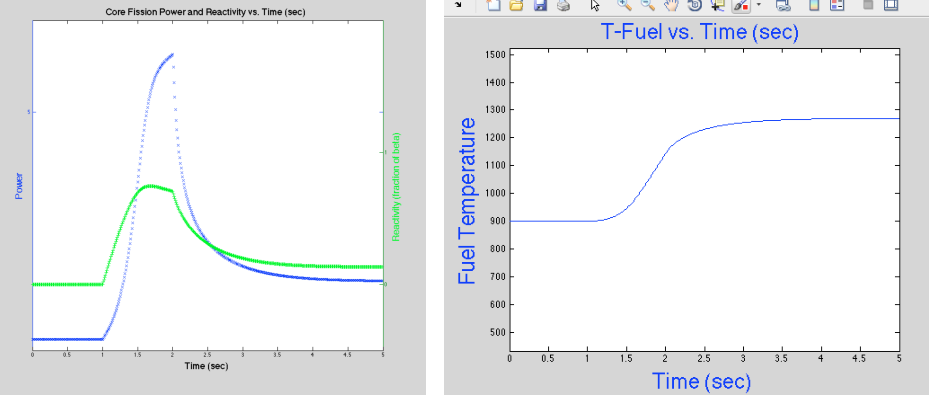
\includegraphics[width=4in]{images/pke/fn3.png}
    \caption{\$1.8 Insertion at Full Power using IK with Feedback}
  \end{figure}

\item As in Fig.~\ref{fn4}, about 3\% of the energy deposited into the coolant (about $2.5 \times 2$ MeV $=$5 MeV worth of neutrons from 200 MeV just from neutron slowing down that is deposited into the coolant), hence the coolant temperature would change slightly as well. Net reactivity comes back to zero.
  \begin{figure}[ht] 
    \centering
    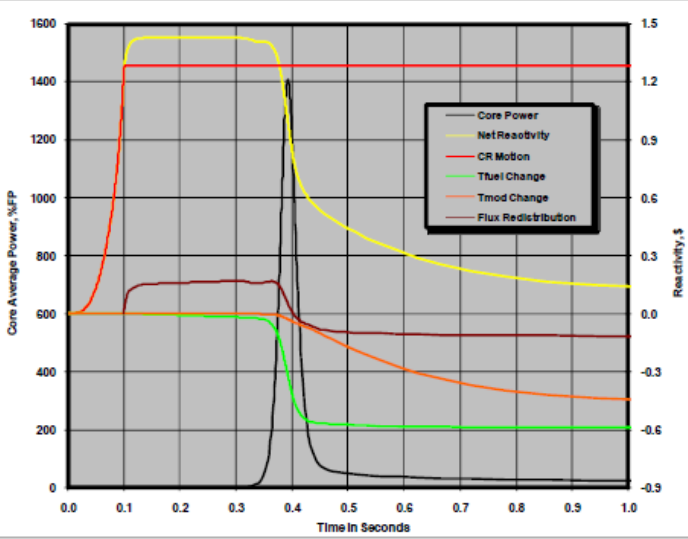
\includegraphics[width=4in]{images/pke/fn4.png}
    \caption{PWR Reactivity Insertion Accident} \label{fn4}
  \end{figure}

\item RIA Safety Analysis: Rod Ejection at HZP. If we have a 1.5\$ RIA without feedback, the power increases very rapidly with an asymptotic period. With Doppler feedback, the feedback is pronound when reactivity is above 1 dollar. A second peak is the characteristic of longer rod change. 
\end{enumerate}

\clearpage
\topic{PKEs with Simple Feedback}
Now we turn away from Fuchs-Nordheim and add some very simple feedbacks into PKEs. We have two first order ODEs, one for $T_{fuel}$, one for $T_{coolant}$. Basically each equation has a source term and a sink term. 
\begin{align}
\ddt T_{fuel} (t) &= a P(t) - b [T_{fuel}(t) - T_{coolant}(t)] \\
\ddt T_{coolant} (t) &= c [T_{fuel}(t) - T_{coolant} (t) ] - d [T_{coolant} (t) - T_{inlet} (t) ] 
\end{align}
Re-write in matrix form, 
\begin{align}
\ddt \left[ \begin{array}{c} T_{fuel}(t) \\ T_{coolant} (t) \end{array} \right]
+ \left[ \begin{array}{cc} b & -b \\ -c & c+d \end{array} \right] 
\left[ \begin{array}{c} T_{fuel} (t) \\ T_{coolant} (t) \end{array} \right] 
= 
\left[ \begin{array}{c} a P_{fuel}(t) \\ d T_{inlet}(t) \end{array} \right]
\end{align}
Using integrating factors to solve the above first order ODE system,  we get, 
\begin{align}
 \left[ \begin{array}{c} T_{fuel}^{n+1} \\ T_{coolant}^{n+1} \end{array} \right]
&= \exp \left\{ -  \left[ \begin{array}{cc} b & -b \\ -c & c+d \end{array} \right] \Delta_t^n \right\}
\left[ \begin{array}{c} T_{fuel}^n \\ T_{coolant}^n \end{array} \right] \\
&+ \exp \left\{ -  \left[ \begin{array}{cc} b & -b \\ -c & c+d \end{array} \right] \Delta_t^n \right\}
\left[ \begin{array}{cc} b & -b \\ -c & c+d \end{array} \right]^{-1}
\exp \left\{ \left[ \begin{array}{cc} b & -b \\ -c & c+d \end{array} \right] \Delta_t^n \right\}
\left[ \begin{array}{c} a P_{fuel}^{n+1} \\ d T_{inlet}^{n+1} \end{array} \right]
\end{align}
We make use of that we know at full power,  flow rate is 30 W/g, $C_p = 300$J/kg-s, $\alpha = -3$ pcm/K, $V_{coolant} = 2 \m/\s, T_{inlet}^0 = 540 \K, T_{coolant}^0 = 560 \K, T_{fuel}^0 = 900 \K$, core height is 4m. 


If power is increasing, we can do TH first and then neutronics. If power is decreasing, 




\clearpage
\topic{Examples of PKEs with Simple Feedbacks}
\begin{enumerate}
\item Ramp reactivity inertion of $0.5\beta$ with feedback. The power decreases because of Doppler feedback and of delayed neutrons. 

\begin{figure}[ht]
  \centering
  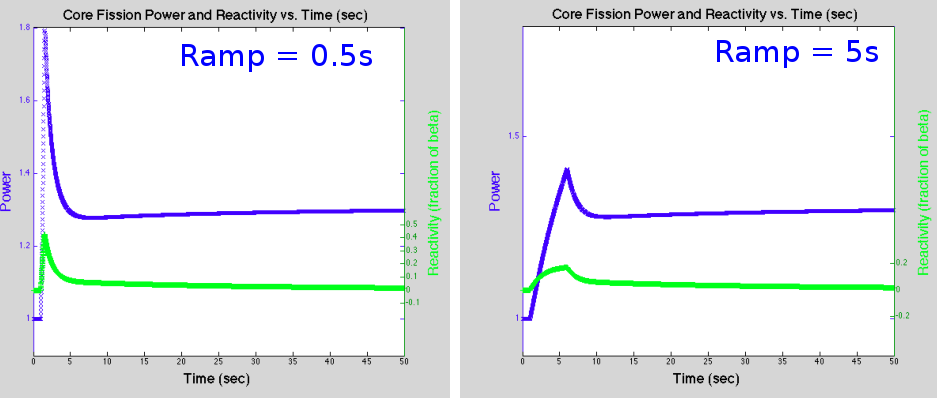
\includegraphics[width=6in]{images/pke/fn5.png}
  \caption{$0.5 \beta$ Reactivity Insertion with Feedback}
\end{figure}

\item Ramp reactivity removal of $0.5\beta$ with feedback. 
\begin{figure}[ht]
  \centering
  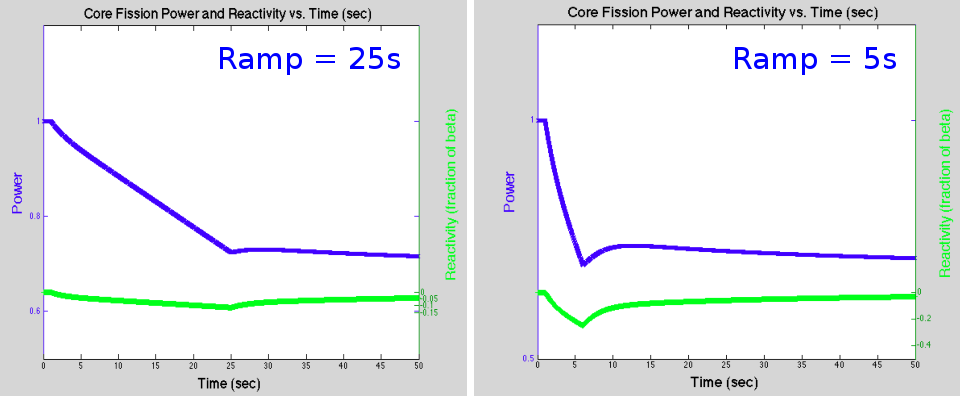
\includegraphics[width=6in]{images/pke/fn6.png}
  \caption{$-0.5 \beta$ Reactivity Insertion with Feedback}
\end{figure}
The slower ramping results in smaller reactivity change (hence smaller peak reactivity for reactivity insertion and larger power dip for negative reactivity insertion), thus smaller power change as well. That is, \textbf{The smaller rate of reactivity change is, the smaller the overshoot is.} But the final/asymptotic results are independent of rate of reactivity insertion, because system always finds stable state. 

Selective ramp insertion: 2 sec, power comes down quickly and recoveries, the radial heat gets high, close to an DNDF failure, makes sure to take into account the power rise. 

Again the asymptotic power level is independent of reactivity changing rate. 


\item 1.5 $\beta$ RIA from HZP with feedback. Power increases by about 100 times. 


\item 1.5 $\beta$ RIA from HFP with feedback. Power increases by about 70 times. Because we start at a higher power region, so we get feedback more quickly this way. The $\Delta T$ is about the same as the HZP because of the reactivity change is the same and our Doppler feedback coefficient is linear. 

\item 1.5 $\beta$ RIA  


\item $1.5 \beta$ bank withdrawal RIA from HFP with feedback: the ejection is so slow that the reactor is at equilibrium the whole time. 
\end{enumerate}
Take-away: we don't really care about the temperal difference/integration, because the asymptotic temperature only depends on the reactivity change, not on the time dependent behavior. 



\clearpage
\topic{Summary}
\begin{enumerate}
\item PKEs assume you are solving for the core average properties; PKEs assume flux spatial shape is constant. Thus PKEs are not very precise for large spatial flux changes. 
\item Peak temperature are proportionally larger than core average properties;
\item If we relly want spatial dynamics, we need to do 3D spatial dynamics to get correct predictions to complicated problems. 
\end{enumerate}
This thermal hydraulics model we have is very crude. For one thing, it has a huge diffusive property, that is, it would not predict any thermal shock behavior. 

\end{document}

\documentclass{school-22.211-notes}
\date{May  2, 2012}

\begin{document}
\maketitle

\lecture{Nodal Diffusion Methods} \label{nodal-methods}
\topic{3D Core Analysis Overview}
Reference: \href{www.oecd-nea.org/dbprog/documents/MC03Smith.pdf}{`Reactor Core Methods' by Smith, MC 2003}. 
There are a couple levels of complexity for performing 3D core analysis,
\begin{itemize}
\item One reactor at one state point: couple core neutronics/fuel heat conduction/coolant hydraulics/structural mechanics for 60,000 fuel pins and 100 axial levels to evaluate thermal margins;
\item Repeat for 50 depletion states and track 300 isotopes;
\item Repeat for 10,000s limiting conditional simulations and 100s of transient accident simulations for safety analysis;
\item Repeat for 1000s of startup and maneuver simulations;
\item Repeat for millions of cycle depletion simulation for designing loading design and optimization;
\item For operator training simulator in real time, 24/7 operation at 5-10 Hz. 
\end{itemize}
The challenges for 3D core calculation include,
\begin{itemize}
\item Predict pin power, axial shapes of pin power: as in Figure~\ref{3Dcore}, the spacers depress the flux. Though even without the spacers, the axial shape would still be more towards the bottom compare with a cosine shape due to the temperature coefficients; 
\item Predict core reactivity with core burnup: as in Figure~\ref{3Dcore}, burnable poisons deplete as burnup increases;
\item Predict in-core detector response;
\item Predict control rod worths and temperature coefficients. 
\end{itemize}
\begin{figure}[ht]
  \centering
  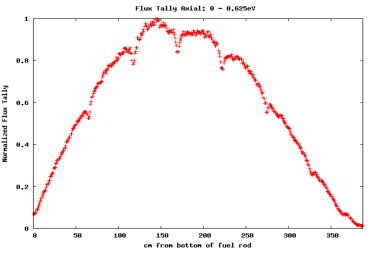
\includegraphics[width=3in]{images/methd/3Dcore-spacer.png}
  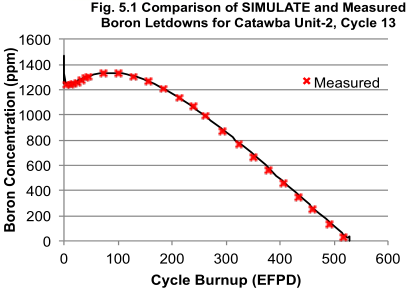
\includegraphics[width=3in]{images/methd/3Dcore-poison.png}
  \caption{3D Core Calculation Samples} \label{3Dcore}
\end{figure}

Approaches to 3D core problems:
\begin{enumerate}
\item S$_N$ Method: computational time problem. We are looking at 100 mesh per pin, 60,000 pins per core, 100 axial mesh, 100 energy groups, 1000 angles, that's about $6 \times 10^{13}$ unknowns. So even with perfect scaling, we are looking at 100,000 core hours for a full core, not to mention feedback, cross section evaluations, boron and control rod searches to critical, etc. Hence S$_N$ has never been done for a single LWR core. 

\item Pin-by-pin diffusion with homogenized pin cells: accuracy problem. There are only $6 \times 10^8$ unknowns, because we only have 1 mesh per pin instead of 100, and 1 angle instead of 1000. It brings the computing time down to 1 hour, but pin homogenization causes a loss of accuracy around strong absorbers. This is now a tractable problem, but not used for production.

\item Nodal method: this is what production codes typically use. There is a huge push towards nodal method, because nodal methods take a mesh size of 20cm to be accurate, whereas Finite Difference method requires a mesh size of about 1 cm. 
\end{enumerate}

\clearpage
\topic{Derivation of Nodal Methods}
Reference: Sutton and Aviles' `Diffusion Theory Methods for Spatial Kinetics Calculations' (1996). 
\begin{enumerate}
\item We start from 3D steady-state multigroup neutron diffusion equation, 
  \eqn{\divergence \vecJ_g(\vecr, E) + \Sigma_{rg} \psi_g (\vecr, E) = \frac{1}{\keff} \chi_g \Sum_{g' = 1}^G \nu \Sigma_{fg'} \psi_{g'}(\vecr, E) + \Sum_{g'=1}^G \Sigma_{sg'g} \psi_{g'}(\vecr, E) }
  Apply Fick's Law of diffusion for current out of flux, 
  \eqn{ \vecJ_g(\vecr, E) = - D_g(\vecr, E) \gradient \psi_g(\vecr, E) }

\item Assumptions: properties are constant in homogenized nodes. Then we find the volume-averaged terms for each node; that is, we integrate over the node volume and then divide by volume,

\item Volume average of diffusion equation for a node: we integrate every term over the node volume then divide by volume. The volume averaged flux becomes, 
  \eqn{ \bar{\psi} = \frac{1}{h_x h_y h_z} \int_0^{h_x} \int_0^{h_y} \int_0^{h_z} \psi(x,y,z) \dx \dy \dz }
  The leakage term becomes (after integrating the divergence term using Gauss Theorem), 
  \eqn{ \int_0^{h_x} \int_0^{h_y} \int_0^{h_z} \divergence \vecJ_g \dx \dy \dz &= \int_0^{h_y} \int_0^{h_z} (J_x(h_x,y,z) - J_x(0,y,z)) \dy \dz  \\
&+ \int_0^{h_x} \int_0^{h_z} (J_y (x,h_y, z) - J_y(x,0,z)) \dx \dz \\
&+ \int_0^{h_x} \int_0^{h_y} (J_z(x,y,h_z) - J_z(x,y,0)) \dx \dy }
  If we define surface-averaged currents, 
  \eqn{ \bar{J}_{gxl} &= \frac{1}{h_y h_z} \int_0^{h_y} \int_0^{h_z} J_x(0,y,z) \dy \dz, & \bar{J}_{gxr} &= \frac{1}{h_y h_z} \int_0^{h_y} \int_0^{h_z} J_x(h_x,y,z) \dy \dz }
  Then the leakage term becomes, 
  \eqn{ \Sum_{u=x,y,z} \frac{\bar{J}_{gur} - \bar{J}_{gul}}{h_u} }
  Together, the nodal balance equation with average terms is, 
  \eqn{ \Sum_{u=x,y,z} \frac{\bar{J}_{gur} - \bar{J}_{gul}}{h_u} + \Sigma_{rg} \bar{\psi}_g &= \frac{1}{\keff} \chi_g \Sum_{g'=1}^G \nu \Sigma_{fg'} \bar{\psi}_{g'} + \Sum_{g'=1}^G \Sigma_{sg'g} \bar{\psi}_{g'} \label{nodal-balance} }
  Notice, 
  \begin{itemize}
    \item The six surface-averaged currents are required to find the node-averaged flux which would determine nodal power;
    \item Surface-averaged currents are average of flux derivative on a surface, which equals derivative of average flux at the surface; 
    \item It is more efficient to work with diffusion equation for average flux rather than solving the diffusion equation for the point-wise fluxes in 3D. 
  \end{itemize}

\item Transverse Integration: we need a set of equations for the surface average currents instead of solving 3D finite different equations directly. To do so, we pick a direction of interest (eg., x direction), and perform integration within node over 2D plane normal to that direction (eg., the grey surface in Figure~\ref{nodal-current}), then devide by the planar area. The LHS of Eq.~\ref{nodal-balance} becomes, 
  \eqn{\Sum_{u=x,y,z} \frac{\bar{J}_{gur} - \bar{J}_{gul}}{h_u} + \Sigma_{rg} \bar{\psi}_g = \frac{1}{h_y h_z} \int_0^{h_z} \int_0^{h_y} (\divergence \vecJ_g(\vecr, E) + \Sigma_{rg} \psi_g (\vecr, E) ) \dy \dz }
\begin{figure}[ht]
  \centering
  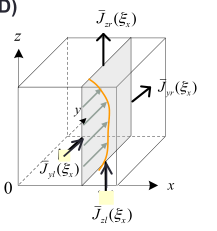
\includegraphics[width=0.28\textwidth]{images/methd/nodal-current.png}
  \caption{Integrate Within Node Over 2D Plane Normal to x-direction} \label{nodal-current}
\end{figure}
  \begin{enumerate}
  \item Define dimensionless independent variables,
    \eqn{ \xi_x &= \frac{x}{h_x}, & \xi_y &= \frac{y}{h_y}, & \xi_z &= \frac{z}{h_z} }
    and we can transform the integration and the derivative operator as well, 
    \eqn{ \frac{\du}{h_u} &= \derivative \xi_u, & \ddu &= \frac{1}{h_u}\frac{\derivative}{\dxi_u}, & u&= x,y,z}

  \item Simplify the averaging with dimensionless variables,
    \eqn{ J_{xgl} &= \int_0^1 \int_0^1 J_x(0,\xi_y, \xi_z) \dxi_y \dxi_z, &J_{gxr} &= \int_0^1 \int_0^1 J_x(1,\xi_y, \xi_z) \dxi_y \dxi_z }
    \eqn{ \bar{\psi} &= \int_0^1 \int_0^1 \int_0^1 \psi(\xi_x, \xi_y, \xi_z) \dxi_x \dxi_y \dxi_z }

  \item The normalized 3D diffusion equation becomes, 
    \eqn{ \left( - \Sum_{u=x,y,z} \frac{D_g}{h_u^2} \frac{\partial^2}{\partial \xi_u^2} + \Sigma_{rg} \right) \psi_g(\xi_x, \xi_y, \xi_z) &=  \frac{1}{\keff} \chi_g \Sum_{g'=1}^G \nu \Sigma_{fg'}\psi_g(\xi_x, \xi_y, \xi_z) + \Sum_{g'=1}^G \Sigma_{sg'g} \psi_g(\xi_x, \xi_y, \xi_z) }

  \item We look at the leakage term after the transverse integration, 
    \begin{align}
      &\int_0^1 \int_0^1 \divergence \vecJ \dxi_y \dxi_z = \int_0^1 \int_0^1 \left( \frac{1}{h_x} \frac{\partial J_x}{\partial \xi_x} + \frac{1}{h_y} \frac{\partial J_y}{\dxi_y} + \frac{1}{h_z} \frac{\partial J_z}{\dxi_z} \right) \dxi_y \dxi_z \\
      &= \int_0^1 \int_0^1 \left( -\frac{D_g}{h_x^2} \frac{\partial^2 \psi}{\partial \xi_x^2} + \frac{1}{h_y} \frac{\partial J_y}{\dxi_y} + \frac{1}{h_z} \frac{\partial J_z}{\dxi_z} \right) \dxi_y \dxi_z \\
      &= - \frac{D_g}{h_x^2} \frac{\partial^2 }{\partial \xi_x^2} \int_0^1 \int_0^1 \psi(\xi_x, \xi_y, \xi_z) \dxi_y \dxi_z \\
      &+ \frac{1}{h_y} \int_0^1 (J_y(\xi_x, 1, \xi_z) - J_y(\xi_x, 0, \xi_z) )\dxi_z + \frac{1}{h_z} \int_0^1 (J_z(\xi_x, \xi_y, 1) - J_z(\xi_x, \xi_y, 0) ) \dxi_y \\
      &= - \frac{D_g}{h_x^2} \frac{\partial \bar{\psi}_x (\xi_x)}{\partial \xi_x^2} + \frac{\bar{J}_{yr}(\xi_x) - \bar{J}_{yl} (\xi_x)}{h_y} + \frac{\bar{J}_{zr} (\xi_x) - \bar{J}_{zl} (\xi_x)}{h_z} 
    \end{align}
    where we defined the \textbf{plane-averaged 1D flux},
    \eqn{\bar{\psi}_x = \int_0^1 \int_0^1 \psi(\xi_x, \xi_y, \xi_z) \dxi_y \dxi_z }
    and \textbf{line-averaged surface current} at an arbitrary position $\xi_x$, 
    \eqn{ \bar{J}_{yr} (\xi_x) &= \int_0^1 J_y(\xi_x, 1, \xi_z) \dxi_z, &\bar{J}_{yl}(\xi_x) &= \int_0^1 J_y(\xi_x, 0, \xi_z) \dxi_z }
    \eqn{ \bar{J}_{zr} (\xi_x) &= \int_0^1 J_z(\xi_x, \xi_y, 1) \dxi_y, &\bar{J}_{zl}(\xi_x) &= \int_0^1 J_z(\xi_x, \xi_y,  0) \dxi_y }

  \item Collect all the terms, we get the transverse integration of 3D diffusion equation, 
    \eqn{ \Sum_{u=y,z} \frac{\bar{J}_{gur}(\xi_x) - \bar{J}_{gul}(\xi_x)}{h_u} - \frac{D}{h_x^2} \frac{\derivative^2}{\dxi_x^2} \bar{\psi}_{gx} (\xi_x) + \Sigma_{rg} \bar{\psi}_{gx} (\xi_x) &=  \frac{1}{\keff} \chi_g \Sum_{g'=1}^G \nu \Sigma_{fg'}\psi_g(\xi_x) + \Sum_{g'=1}^G \Sigma_{sg'g} \psi_g(\xi_x)  }
    If we define a \textbf{transverse leakage term} and move it to the RHS, 
    \eqn{ L_{gu}(\xi_x) &= \frac{1}{h_u} \left( \bar{J}_{gur}(\xi_x) - \bar{J}_{gul}(\xi_x) \right), & u &= y,z }
    and also define the \textbf{diffusion equivalent group constant}, 
    \eqn{ \Sigma_{Dg}^x  = \frac{D}{h_x^2} }
    We get the transverse integrated 1D diffusion equation,
    \eqn{ - \Sigma_{Dg}^x \frac{\derivative^2}{\dxi_x^2} \bar{\psi}_{gx} (\xi_x) + \Sigma_{rg} \bar{\psi}_{gx} (\xi_x) = \frac{1}{\keff} \chi_g \Sum_{g'=1}^G \nu \Sigma_{fg'} \bar{\psi}_{g'x} (\xi_x) + \Sum_{g'=1}^G \Sigma_{sg'g} \bar{\psi}_{g'x} (\xi_x) - L_{gy} (\xi_x) - L_{gz} (\xi_x)  } 

  \item Repeat for the other two directions, we get a set of 3 directional 1D diffusion equations.
    \begin{align}
      \boxed{ - \Sigma_{Dg}^x \frac{\derivative^2}{\dxi_x^2} \bar{\psi}_{gx} (\xi_x) + \Sigma_{rg} \bar{\psi}_{gx} (\xi_x) = \frac{1}{\keff} \chi_g \Sum_{g'=1}^G \nu \Sigma_{fg'} \bar{\psi}_{g'x} (\xi_x) + \Sum_{g'=1}^G \Sigma_{sg'g} \bar{\psi}_{g'x} (\xi_x) - L_{gy} (\xi_x) - L_{gz} (\xi_x) } \notag \\
   \boxed{ - \Sigma_{Dg}^y \frac{\derivative^2}{\dxi_y^2} \bar{\psi}_{gy} (\xi_y) + \Sigma_{rg} \bar{\psi}_{gy} (\xi_y) = \frac{1}{\keff} \chi_g \Sum_{g'=1}^G \nu \Sigma_{fg'} \bar{\psi}_{g'y} (\xi_y) + \Sum_{g'=1}^G \Sigma_{sg'g} \bar{\psi}_{g'y} (\xi_y) - L_{gz} (\xi_y) - L_{gx} (\xi_y) }  \notag \\
     \boxed{ - \Sigma_{Dg}^z \frac{\derivative^2}{\dxi_z^2} \bar{\psi}_{gz} (\xi_z) + \Sigma_{rg} \bar{\psi}_{gz} (\xi_z) = \frac{1}{\keff} \chi_g \Sum_{g'=1}^G \nu \Sigma_{fg'} \bar{\psi}_{g'z} (\xi_z) + \Sum_{g'=1}^G \Sigma_{sg'g} \bar{\psi}_{g'z} (\xi_z) - L_{gx} (\xi_z) - L_{gy} (\xi_z) } \notag
    \end{align}

  \item Interpretations: we turn a 3D partial differential equation into three 1D ordinary differential equation that are coupled through average transverse leakage term. It is exact if the transverse leakage shape is known. 
  \end{enumerate}

\item Approximation on transverse leakage: from observation, flux is insensitive to the transverse leakage shape, so we are going to perform a quandrature polynomial with 2nd order polynomials of the leakage term, and iteratively update them. Quadratic approximation in each node, 
  \eqn{ L(\xi) = \bar{L} + l_1 P_1(\xi) + l_2 P_2(\xi) }
  We apply average TL conservation scheme to determine $l_1, l_2$. We use three node average transver leakages (the values of each node and its two adjacent nodes), and impose constraint of conserving the averages of two adjacent nodes. About how we handle the rest of this method, we present three methods in the following section. 
\end{enumerate}


%%%%%%%%%%%%%%%%%%%%%%%%%%
\clearpage
\topic{Three Nodal Methods}
\begin{enumerate}
\item Nodal Expansion Method (NEM) developed by Finnemann (KWU 1975). 
  \begin{enumerate}
  \item We approximate 1D flux by 4th order polynomial, 
    \eqn{ \bar{\psi}(\xi) = \Sum_{i=0}^4 a_i P_i (\xi) }
    where the basis functions are, 
    \begin{align}
      P_0(\xi) &= 1 \\
      P_1(\xi) &= 2 \xi - 1\\
      P_2(\xi) &= 6 \xi (1-\xi) - 1 \\
      P_3(\xi) &= 6 \xi (1-\xi)(2\xi-1) \\
      P_4(\xi) &= 6 \xi (1-\xi)(5\xi^2 -5\xi +1)
    \end{align}
    Notice these basis functions are not orthogonal, and integration from 0 to 1 would result in zero. Keep in mind that our transverse leakage is 2nd order (because the result is not very sensitive to the expansion of the transverse leakage). 

  \item BCs: In a two nodes case, we have 16 unknowns from: 4 flux moments $\times$ 2 nodes $\times$ 2 energy groups. But we only have 8 knowns, 
    \begin{itemize}
      \item 4 node average fluxes: 2 groups $\times$ 2 nodes;
      \item 2 interface continuity conditions: from 2 energy groups;
      \item 2 current continuity conditions: from 2 energy groups. 
    \end{itemize}
    Hence we need 8 additional constraints because polynomials can not satisfy the differential equations exactly. 

  \item To find the next 8 constrains, we use \textbf{weighted residual method} for each group in the 1D diffusion equation, 
    \eqn{ \int_0^1 w(\xi) \left( -\Sigma_D \frac{\derivative}{\dxi^2} \psi(\xi) + \Sigma_r \psi(\xi) \right) \dxi = \int_0^1 w(\xi) \left( \frac{1}{\keff} \chi \psi(\xi) + S(\xi) - L(\xi) \right) \dxi }
    The closure relationship basically forces the $P_1, P_2$ integration to go to zero. Forcing the 1st spatial moment of diffusion equation to go to zero gives us, 
    \eqn{ \int_0^1 P_1(\xi) \left( - \Sigma_D \frac{\derivative}{\dxi^2} \psi(\xi) + \Sigma_r \psi(\xi) - Q(\xi) \right) \dxi &= 0, & a_3 &= \frac{5 q_1 + 3 q_3 - 5 a_1 \Sigma_r}{3(60 \Sigma_D + \Sigma_r)} }
    Forcing the 2nd spatial moment of diffusion equation to go to zero gives us, 
    \eqn{ \int_0^1 P_2(\xi) \left( - \Sigma_D \frac{\derivative}{\dxi^2} \psi(\xi) + \Sigma_r \psi(\xi) - Q(\xi) \right) \dxi &= 0, & a_4 &= \frac{-7 q_2 + 3 q_4 + 7 a_2 \Sigma_r}{420(\Sigma_D + 3\Sigma_r)} }    
    Notice we don't know $a_1, a_2$. But we get two pieces of information from the spatial moments. That gives us in total 2 spatial moments $\times$ 2 nodes $\times$ 2 groups $= 8$ constraints. Together that's 16 constraints for 16 unknowns. 

  \item The choice of the weighted residual equations is flexible -- the results are not very sensitive to the weights. For instance, we can choose the same expansion coefficients for $P_i$. 

  \item Two-node 2-group NEM is different from finite-difference methods in terms of: 
    \begin{itemize}
      \item Flux shapes in each group affects coupling equations for other group;
      \item The coupling equations depend on transverse leakages;
      \item Final form of the equations can be made similar to 3D finite difference. 
    \end{itemize}
  \end{enumerate}


\clearpage
\item 2-Group Analytic Nodal Method (ANM) developed at MIT by Henry (1978). 
  \begin{enumerate}
  \item We start from the 1D 2-Group transverse-integrated diffusion equations, and move all terms except the transverse leakage on the LHS, 
    \begin{align}
      -D_1 \frac{\derivative^2 \psi_1(x)}{\dx^2} + \Sigma_{r1} \psi_1(x) - \frac{1}{\keff} (\nu \Sigma_{f1} \psi_1 (x) + \nu \Sigma_{f2} \psi_2 (x) ) &= - L_1(x) \\
      -D_2 \frac{\derivative^2 \psi_2(x)}{\dx^2} + \Sigma_{r2} \psi_2(x) - \Sigma_{12} \psi_1 (x) &= - L_2 (x) 
    \end{align}

  \item The analytic solution is in the form of, 
    \eqn{ \psi_g(x) = \psi_g^H (x) + \psi_g^P (x)}
    where the trial homogeneous solution is, 
    \eqn{ \psi_g^H (x) = \hat{\psi}_g^H \exp(i Bx) }
   
\item We find the homogeneous solution first. The characteristic equation is, 
    \eqn{ \left[ \begin{array}{cc} 
          D_1 B^2 + \Sigma_{r1} - \frac{1}{\keff} \nu \Sigma_{f1} & -\frac{1}{\keff} \nu \Sigma_{f2} \\ 
          -\Sigma_{12} & D_2 B^2 + \Sigma_{r2} 
          \end{array} \right] 
      \left[ \begin{array}{c} 
          \hat{\psi}_1^H \\ \hat{\psi}_2^H 
        \end{array} \right] = 
      \left[ \begin{array}{c} 0 \\ 0 \end{array} \right] }
    For nontrivial solution, we set the determinant to zero, and re-write the expression in terms of $B^2$: 
    \eqn{ (B^2)^2 + \overbrace{\left( \frac{\Sigma_{r1}}{D_1} + \frac{\Sigma_{r2}}{D_2} - \frac{\frac{\nu \Sigma_{f1}}{\keff}}{D_1} \right)}^{2b} B^2 + \overbrace{ \left( 1 - \frac{\kinf}{\keff} \right) \frac{\Sigma_{r1}}{D_1} \frac{\Sigma_{r2}}{D_2} }^{c} = 0 }
    The roots of characteristic equations are the \textbf{eigen-buckling}; more specifically, one of them is the \hi{fundamental mode}, and the other is the \hi{harmonic mode}\footnote{recall quadratic roots for $ax^2 + bx + c = 0$ are $x = \frac{-b \pm \sqrt{b^2 - 4ac}}{2a}$}, 
    \begin{align}
      &\mbox{Fundamental Mode} &B_1^2&= b\left(-1 + \sqrt{1 - \frac{c}{b^2}} \right) = \left\{ \begin{array}{cc} > 0 & \kinf > \keff \\ < 0 & \kinf < \keff \end{array} \right. \\
      &\mbox{Harmonic Mode} &B_2^2&=b\left(-1 - \sqrt{1 - \frac{c}{b^2}} \right) <0
    \end{align}
    The homogeneous solution for group $g$ is: 
     \begin{align}
      &\mbox{Fundamental Mode} &\psi_{g1}^H(x)&= \left\{ \begin{array}{cc} a_{g1} \sin(B_1 x) + a_{g2} \cos(B_1x) & \kinf > \keff \\ a_{g1} \sinh(B_1 x) + a_{g2} \cosh(B_1 x) & \kinf < \keff \end{array} \right. \\
      &\mbox{Second-Harmonic Mode} &\psi_{g2}^H&=a_{g3} \sinh(B_2 x) + a_{g4} \cosh(B_2 x) 
    \end{align}   
     The combined homogeneous solution shows that group 1 and group 2 equations are linearly dependent, 
     \eqn{ \left[ \begin{array}{c} \psi_1^H(x) \\ \psi_2^H (x) \end{array} \right] = \left[ \begin{array}{c} a_{11} \sin(B_1 x) + a_{12} \cos (B_1 x) \\ a_{21} \sinh(B_2 x) + a_{22} \cosh(B_2 x) \end{array} \right] =  \left[ \begin{array}{cc} r_1 & r_2 \\ 1 & 1 \end{array} \right] \left[ \begin{array}{c} a_{21} \sin(B_1 x) + a_{22} \cos (B_1 x) \\ a_{23} \sinh(B_2 x) + a_{24} \cosh(B_2 x) \end{array} \right] }
     where the fast-to-thermal flux ratio is defined as,
     \eqn{ r_m &= \frac{a_{11}}{a_{21}} = \frac{a_{12}}{a_{22}} = \frac{D_2 B_m^2 + \Sigma_{r2}}{\Sigma_{12}} }

\item Next we find the particular solution, which is determined solely by quadratic transverse leakage, 
  \eqn{ \psi_g^P (\xi) = c_{0g} + c_{1g} P_1(\xi) + c_{2g} P_2(\xi) }
  where  
\eqn{ \left[ \begin{array}{c} c_{1p} \\ c_{2p} \end{array} \right] &= A^{-1} \left[ \begin{array}{c} -b_{1p} \\ -b_{2p} \end{array} \right], &p &=1,2.
 &\left[ \begin{array}{c} c_{10} \\ c_{20} \end{array} \right] &= A^{-1} \left[ \begin{array}{c} -b_{10} + 6 D_1 c_{12} / \Delta x^2 \\ -b_{20} + 6 D_2 c_{22} / \Delta x^2 \end{array} \right]. }


\item Hence the general solution in a node is, 
     \eqn{ \left[ \begin{array}{c} \psi_1^H(x) \\ \psi_2^H (x) \end{array} \right] = \left[ \begin{array}{cc} r_1 & r_2 \\ 1 & 1 \end{array} \right] \left[ \begin{array}{c} a_{21} \sin(B_1 x) + a_{22} \cos (B_1 x) \\ a_{23} \sinh(B_2 x) + a_{24} \cosh(B_2 x) \end{array} \right] + \left[ \begin{array}{c} \psi_1^P(x) \\ \psi_2^P (x) \end{array} \right] }
     That is, we have 4 coefficients to determine for a 2 group problem. 
     
   \item BCs: quadratic transverse leakage for two nodes, node-average fluxes for two nodes. We have 8 unknown coefficients (4 per node times 2 nodes), and we have 9 constraints coming from: 
     \begin{itemize}
       \item 4 node-averaged fluxes: 2 groups times 2 nodes;
       \item 2 flux interface continuity from 2 energy groups;
       \item 2 current interface continuity from 2 energy groups.
     \end{itemize}
     Hence there is no need for weighted residual equations because we have the exact solution to the 1D diffusion equation. Then all groups are solved simultaneously.

   \item Pros and Cons: no need for weighted residual equations because we have exact solution to the 1D diffusion equation. The drawback is, all groups are solved simultaneously, so the generalization is very hard. But with the help of modal expansion, now we can do ANM for any number of energy groups. 
  \end{enumerate}

\clearpage
\item Semi-Analytic Nodal Method (SANM) developed at Studsvik (1985). 
  \begin{enumerate}
  \item SANM uses NEM equations for the fast group, and performs transverse integrated 1D neutron diffusion equation for the thermal group, 
    \eqn{ -D_2 \frac{\derivative^2}{\dx^2} \psi_2(x) + \Sigma_{r2} \psi_2(x) &= \Sigma_{s12} \psi_1(x) - L_{y2} (x) = Q_2 (x) }

  \item We approximate the source $Q$ with 4th order Legendre Polynomial, 
    \eqn{ Q_g(x) = \Sum_{i=0}^4 q_i P_i\left(\frac{2x}{h}\right) }
    
  \item The analytic solution of thermal group diffusion equation is, 
    \eqn{ \psi_g(x) &= A \sinh(\kappa_g x) + B \cosh(\kappa_g x) + \Sum_{i=0}^4 c_i P_i \left(\frac{2x}{h}\right), &\kappa_g&=\sqrt{\frac{\Sigma_g}{D_g}} }
    We end up with \textit{exponential homogeneous solution and polynomial particular solution}. 

\item We differentiate to get expression for net current at the interface: 
    \eqn{ J_g(x) &= -D_g \ddx \psi_g(x) }
    We use the continuity of net currents/flux to get analytic expression for coupling. 
    \begin{figure}[ht]
      \centering
      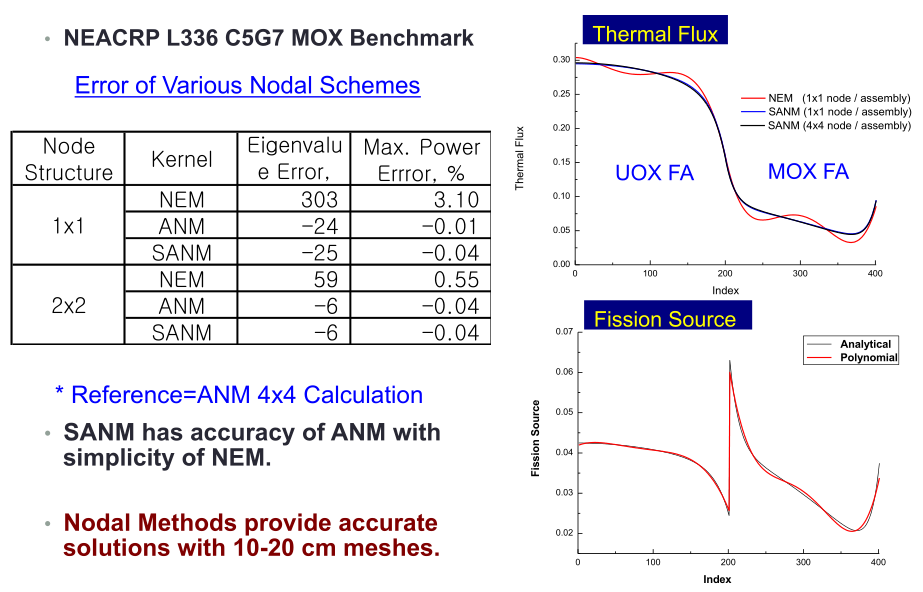
\includegraphics[width=5in]{images/methd/SANM-accuracy.png}
      \caption{Accuracy of SANM in Two-Group Application}
    \end{figure}
  \end{enumerate}
\end{enumerate}


\clearpage
\topic{Iterative Solution Technique}
In this section we show how the three nodal methods come down to be pretty much the same. The classic solution sequance involves,
\begin{enumerate}
\item Guess $\keff$, approximate transverse leakages as zero.
\item Evaluate all coupling terms for 1-node equation,
  \eqn{ \left[ \begin{array}{c} J_1 \\ J_2 \end{array} \right] = \left[ \begin{array}{cc} a_{11} & a_{12} \\ a_{21} & a_{22} \end{array} \right] \left[ \begin{array}{c} \bar{\psi}_1^+ \\ \bar{\psi}_2^+ \end{array} \right]  - \left[ \begin{array}{cc} b_{11} & b_{12} \\ b_{21} & b_{22} \end{array} \right] \left[ \begin{array}{c} \bar{\psi}_1^- \\ \bar{\psi}_2^- \end{array} \right] + \Sum_{m=1,4} \left[ \begin{array}{cc} c_{11} & c_{12} \\ c_{21} & c_{22} \end{array} \right] \left[ \begin{array}{c} L_{m1} \\ L_{m2} \end{array} \right] }

\item Setup global matrix equation,
\eqn{ \left[ \begin{array}{cccc} 
 [A] & [B] & [C] & [D] \\
 \left[E\right] & [1] & [F] & [G] \\
 \left[H\right] & [I] & [1] & [J] \\
 \left[K\right] & [L] & [M] & [1] \\
\end{array} \right]  
\left[ \begin{array}{c} 
[\bar{\psi} ] \\ 
\left[L_x\right] \\ 
\left[L_y\right] \\ 
\left[L_z\right] \end{array} \right] = \frac{1}{\keff} 
\left[ \begin{array}{cccc} 
[m] & [0] & [0] & [0] \\ 
\left[0\right] & [0] & [0] & [0] \\ 
\left[0\right] & [0] & [0] & [0] \\ 
\left[0\right] & [0] & [0] & [0] 
\end{array} \right] 
\left[ \begin{array}{c} 
[\bar{\psi} ] \\ 
\left[L_x\right] \\ 
\left[L_y\right] \\ 
\left[L_z\right] \end{array} \right] }

\item We solve the 3D balance equation by fission source and flux/leakage iteration, similar to finite difference, but leakate term has group-to-group coupling. 

\item Update $\keff$ and return to 2 until converged. 
\end{enumerate}

Next \textbf{the non-linear iterative solution} sequence was developed,
\begin{enumerate}
\item  Guess $\keff$, solve the standard 3D finite difference equations. 

\item Evaluate all interface currents from 2-node equations,
  \eqn{ \left[ \begin{array}{c} J_1 \\ J_2 \end{array} \right] = \left[ \begin{array}{cc} a_{11} & a_{12} \\ a_{21} & a_{22} \end{array} \right] \left[ \begin{array}{c} \bar{\psi}_1^+ \\ \bar{\psi}_2^+ \end{array} \right]  - \left[ \begin{array}{cc} b_{11} & b_{12} \\ b_{21} & b_{22} \end{array} \right] \left[ \begin{array}{c} \bar{\psi}_1^- \\ \bar{\psi}_2^- \end{array} \right] + \Sum_{m=1,4} \left[ \begin{array}{cc} c_{11} & c_{12} \\ c_{21} & c_{22} \end{array} \right] \left[ \begin{array}{c} L_{m1} \\ L_{m2} \end{array} \right] }
It's almost finite difference, but higher order in the sense that we say if flux has already converged, what would the current be. 

\item Redefine equivalent coupling terms to preserve nodal solution for current. Notice the coefficients $\alpha, \beta, \gamma, \delta$ are non-linear functions of the solution. 
  \eqn{ \left[ \begin{array}{c} J_1 \\ J_2 \end{array} \right] = \left[ \begin{array}{cc} \alpha & 0 \\ 0 & \gamma \end{array} \right] \left[ \begin{array}{c} \bar{\psi}_1^+ \\ \bar{\psi}_2^+ \end{array} \right]  
- \left[ \begin{array}{cc} \beta & 0 \\ 0 & \delta \end{array} \right] \left[ \begin{array}{c} \bar{\psi}_1^- \\ \bar{\psi}_2^- \end{array} \right] }

\item Set up global matrix equation,
  \eqn{ [A] [[\bar{\psi}]] = \frac{1}{\keff} [M] [[\bar{\psi}]] }

\item Solve 3D balance equations by fission source and flux iteration (same as finite-difference, and no group-to-group spatial coupling term). 

\item Update $\keff$ and return to 2 until converged. 
\end{enumerate}
This method is almost the same as CMFD, but with slightly different coefficients $\alpha, \beta, \gamma, \delta$. The point is, whether we do any one of the three nodal methods, we get a slightly different net current, the rest of the iteration looks the same. Mechanically, it is the same as the two-node two-group finite difference solution that we've already done. 



\clearpage
\topic{Summary of Transverse Integration Methods}
\begin{enumerate}
\item Transverse integration method is an innovative way to solve 3D diffusion equation by converting 3D PDE into 3 ODEs: 
  \begin{itemize}
    \item Solutions are only weakly dependent on the leakage shapes;
    \item Transverse leakage is approximated by a second order polynomial and iteratively updated.
  \end{itemize}

\item NEM is simple and efficient; it facilitates multi-group calculations, but loses accuracy for highly varying flux problems. 

\item ANM has the best accuracy, but it is not easy (though has been done) for general multi-group problems.

\item SANM is the most practical for LWR applications, because it has simple algebra, is multi-group applicable, and is comparable in accuracy to ANM. 

\item Non-linear solution method (eg, iterative) can be easily applied to all three methods. 
\end{enumerate}



\end{document}

\documentclass{school-22.211-notes}
\date{May  7, 2012}

\begin{document}
\maketitle

\lecture{Homogenization Methods} \label{homogenization}
We continue our discussion on nodal methods, and would cover spatial dependency of cross sections and homogenization methods. This lecture follows closely on Smith's `Assembly Homogenization Techniques for Light Water Reactor Analysis' (Prog. in Nulear Energy, 1986). 




\topic{Spatial Dependence of Nodal Cross Sections}
\begin{enumerate}
\item Spatial configuration of nodal cross sections matters because of the following three terms vary with respect to space:
\begin{itemize}
\item Burnup gradients: cross sections vary quadratically with respect to exposure, and we integrate bundle surface burnups;

\item Fuel temperature gradients $\to$ Doppler feedback: fuel temperature is related to the local fission rate; and Doppler feedback is from fuel temperature variations;

\item Non-uniform density gradients $\to$ coolant feedback: coolant feedback is caused by density distribution.

\item Spectral interaction between assemblies: for instance, leakage and MOX/UO2 interface depends on cross sections.
\end{itemize}
For instance, if we know the fuel temperature gradient, from any library we know the cross section change with respect to temperature, then we can compue the cross section distribution. Space-dependent nodal xs is very easy to integrate in NEM nodal method, but not so easy with ANM and SANM because of the polynomials. 

\item Space-dependent XS Changes Flux. Recall that for 1 nodal balance equation and 2 incoming current BCs, and the two additional conditions come from the weighted residual method. Now that we add in the spatial dependency of the cross sections, the weighted residual method for 1D neutron diffusion equation remains the same: 
\eqn{ \int_0^1 w(\xi) \left( - \Sigma_D \ddxin2 \psi(\xi) + \Sigma_r (\xi) \psi(\xi) \right) \dxi   \int_0^1 \left( \frac{1}{\keff} \chi(\xi) \psi(\xi) + S(\xi) - L(\xi) \right) \dxi  }
Again, we set the 1st moment of neutron diffusion equation to zero, hence deriving an expression for $a_3$, 
\eqn{ \int_0^1 P_1(\xi) \left( - \Sigma_D \ddxin2 \psi(\xi) + \Sigma_r (\xi) \psi(\xi) - Q(\xi) \right) \dxi &= 0, &a_3&=\frac{5 q_1 + 3 q_3 - 5a_1 \Sigma_r + \cdots}{3(60 \Sigma_D + \Sigma_r) + \cdots} }
Similarly we set the 2nd moment of neutron diffusion equaion to zero, hence deriving an expression for $a_4$, 
\eqn{ \int_0^1 P_2(\xi) \left( - \Sigma_D \ddxin2 \psi(\xi) + \Sigma_r (\xi) \psi(\xi) - Q(\xi) \right) \dxi &= 0, &a_4&=\frac{-7q_2 + 3 q_4 + 7 a_2 \Sigma_r + \cdots}{420(\Sigma_D + 3\Sigma_r) + \cdots} }
Interpretations: flux distribution changes after we add in the spatial dependency of cross sections; but mechanically there is nothing tricky: we are just adding more terms, designated by $\cdots$, to the expressions in the above two equations. 

\item KWU depletion benchmark using BOC-2 Powers: without space-dependent xs, the error on $\keff$ is about 12pcm (on the edge); with space-dependent xs, the error on $\keff$ drops to about 4pcm (on the edge). The error on the interior is always smaller. Basically if we do not model the space-dependent xs, then our assembly is solved using zero current BC and is not accurate when the location and/or the orientation of the assembly is changed. Alternatively we can further sub-divide the node to get a reduced error as well. 
\end{enumerate}

\clearpage
\topic{Homogenization of Fuel Assemblies}
Homogenization can be done on either pins or assemblies. We are mostly going to talk about assembly level because they are harder. 
\begin{enumerate}
\item Given a reference solution, we build a heterogeneous reactor using,
\eqn{ \divergence \vecJ_g(\vecr) + \Sigma_{tg}(\vecr) \phi_g(\vecr) &= \Sum_{g'=1}^G \left( \frac{1}{\keff} M_{gg'} (\vecr) + \Sigma_{gg'} (\vecr) \right) \phi_{g'} (\vecr) }
and analogous equation for the homogenized model using homogenized parameters,
\eqn{ \divergence \hat{\vecJ}_g(\vecr) + \hat{\Sigma}_{tg}(\vecr)\hat{\phi}_g(\vecr) &= \Sum_{g'=1}^G \left( \frac{1}{\keff} \hat{M}_{gg'} (\vecr) + \hat{\Sigma}_{gg'} (\vecr) \right) \hat{\phi}_{g'} (\vecr) }

\item We need to decide what terms to preserve. For instance, if we preserve the scalar flux, reaction rates (for every reaction type and every energy $\alpha = t, gg'$ etc) and the leakage term, $\keff$ will be preserved. 
\begin{align}
\int_{V_i} \hat{\Sigma}_{\alpha g} \hat{\phi}_g \dr &= \int_{V_i} \Sigma_{\alpha g} \phi_g \dr  & \hat{\Sigma}_{\alpha g}^i &= \frac{\int_{V_i} \Sigma_{\alpha g} \phi_g \dr}{\int_{V_i} \hat{\phi}_g \dr} \\
\int_{S_i^k} \divergence \hat{J}_g \dS &= \int_{S_i^k} \divergence \vecJ_g \dS & \hat{J}_g &= - \hat{D}_g \gradient \hat{\phi}_g, \mbox{ where } \hat{D}_g^i = \frac{-\int_{S_i^k} \vecJ_g \dS}{\int_{S_i^k} \gradient \hat{\phi}_g \dS}
\end{align}

\item What happens is that we don't really know the true heterogeneous flux, so we further approximate heterogeneous flux using results from assembly results.
\begin{align}
\int \hat{\phi}_g \dr &= \int \phi_{Ag} \dr  \\
\hat{D}_g^i &= \frac{-\int_{S_i^k} \vecJ_g \dS}{\int_{S_i^k} \gradient \hat{\phi}_{Ag} \dS}
\end{align}
Using the assembly results give us AXS (assembly flux-weighted cross section). 

\item AXS (assembly flux-weighted cross sections): in a HAFAS BWR benchmark case, notice that the error (-0.44\% for $\keff$, 5.5\% for average assembly power) is somewhat independent of the mesh size (1x1 vs. 3x3) and angular expansion (P1 vs. P3), which suggests that \hi{the error comes from homogenization of the cross sections} . 

\item RXS (reference cross sections): the errors mentioned above do not go away neither if we use perfect cross sections (RXS): -0.34\% for $\keff$, 4.1\% for average assembly power. As we will examine in the next section, the errors have to do with the discontinuity of scalar flux. 

\item Flux discontinuity: since the homogenized flux distribution in each node is affected by the diffusion coefficients, and the choice of flux weighted diffusion coefficients is in a sense entirely arbitrary, the interface fluxes can be different as in Figure~\ref{1Dnodal-flux}(c). As a direct result, the homogenized flux in nodes $i, i+1$ when the two-node homogenized diffusion problem is solved with BCs $J_i^-, J_{i+1}^+$ and continuity of flux and current interface conditions would yield Figure~\ref{1Dnodal-flux}(d), which is different from Figure~\ref{1Dnodal-flux}(c). That is, the homogeneous flux is not continuous across the surface anymore. 
\begin{figure}[ht]
  \centering
  \includegraphics[width=4in]{images/methd/1Dnodal-flux.png}
  \caption{Nodal Flux Distribution} \label{1Dnodal-flux}
\end{figure}

\item Heterogeneity factor(HF): Koebke introduced the \hi{Heterogeneity Factor}(Lugano, 1978), which states,
\eqn{ \hat{\phi}_i f_i^+ &= \hat{\phi}_{i+1}^- f_{i+1}^-  \label{nodal-hh}}
where the equivalence factors are defined as (and computed from reference solution), 
\eqn{ f_i^+ &= \frac{\phi_i^+}{\hat{\phi}_i^+}, &f_{i+1}^-&= \frac{\phi_{i+1}^-}{\hat{\phi}_{i+1}^-}}
which says that the heterogeneous flux is continuous across the interface and that there exists a direct relationship between the heterogeneous and homogenized surface fluxes. When the homogenized two-node problem is solved, the homogenized flux is made discontinuous (by a factor of $f_i^+/f_{i+1}^-$) and the homogenized flux distribution will be the same as that in Fig.~\ref{1Dnodal-flux}(c), which results in the \hi{preservation of interface current / net current by adding a degree of freedom which essentially relaxes boundary conditions}. 

\item Nodal equivalence theory and discontinuity factor(DF): Koebke's method of constraining the diffusion coefficients such that the heterogeneity factors are identical on both surfaces of a node requires an iterative method to determine diffusion coefficients. A variation of Koebke's method takes advantage of the fact that exact heterogeneity factors can be defined from Eq.~\ref{nodal-hh} for any value of the diffusion coefficient. Note that unless the diffusion coefficients are found iteratively, the values of the heterogeneity factors on the opposite faces of a node will be different. These two factors are referred to as \hi{discontinuity factor}(DF) to distinguish them from heterogeneity factors, 
  \eqn{ f_{gi,j}^{u-} &= \frac{\phi_{gi,j}^u (u_l)}{\hat{\phi}_{gi,j}^u (u_l)}, &f_{gi,j}^{u+} &= \frac{\phi_{gi,j}^u (u_{l+1})}{\hat{\phi}_{gi,j}^u (u_{l+1})} }
  where $u_l, u_{l+1}$ are the lower and upper $u$-direction boundaries of node $i,j$. 

\item Application of DF: Koebke modified the NEM code, demonstrating that heterogeneous reference solutions could be reproduced by using heterogeneity factors; Smith modifed the QUANDRY code, demonstrating that even CMFD method could reproduce heterogeneous reference solution using discontinuity factors. The updated nodal interface current on the upper $u$-direction surface of node $i,j$ in the CMFD approximation is,
  \eqn{ \hat{J}_{gi,j}^u = \frac{2D_{i,j} D_{i+1,j}}{h_i h_{i+1}} \frac{f_{gi,j}^{u+} \hat{\phi}_{gi,j} - f_{gi+1,j}^{u-} \hat{\phi}_{gi+1,j}}{h (f_{gi+1,j}^{u-} + f_{gi,j}^{u+})} }
  which is different from the traditional CMFD current, 
  \eqn{ \hat{J}_{gi,j}^u = \frac{2D}{h} \left[ \hat{\phi}_{gi,j} - \hat{\phi}_{gi+1,j} \right] }
  Notice the heterogeneity-modified-CMFD is different from the traditional CMFD in the sense that the coefficients in front of the two flux are not the same anymore. 

\item Assembly Discontinuity Factor (ADF). Coming from the realization that the discontinuity factors are not very sensitive to positions etc and mostly dependent on material distribution, we can simply approximate the homogenized results using a single node with homogenized cross section and zero flux boundary condition. That is, there exists a homogeneous analogy to the heterogeneous assembly calculation: a single-node problem with zero net current boundary conditions. In the analogous problem, the homogenized fluxes are spatially flat. Since the assembly-averaged fluxes in the homogeneous and heterogeneous assembly calculations are by definition equal, \textbf{the DFs are simply ratios of the surface-averaged fluxes to the cell-averaged fluxes in the heterogeneous assembly calculation.} Notice this is not true in general; this is just one approximation. 
  \begin{itemize}
  \item It is thus possible to approximate all of the equivalence parameters, assembly discontinuity factors (ADFs), by perfoming assembly calculations for each type of assembly. 
  \item For the HAFAS problem, the ADFs are within a few percent of the mean values of the reference discontinuity factor (RDFs) for all assembly types. Moreover, the fast group DFs are much closer to unity than are the thermal group DFs; the wide gap DFs are much different than the narrow gap DFs. 
  \item The good agreement between ADFs and RDFs suggests that DFs are insensitive to the assembly position, and ADFs can be computed directly from the information available in standard assembly calculations. 
  \item ADFs dramaticaly reduce errors in both PWRs and BWRs. 
  \item The AXS-ADF combination is important in that it is more accurate than either RXS-ADF or AXS-RDF. Part of the reason AXS-ADF is more accurate is that ADF and AXS tend to have erros opposite in signs. Keep in mind that reference xs (RXS) is not sufficient to reduce errors. 
  \end{itemize}


\item ZION benchmark results. Reflector data mostly depends on boron distribution and do not depend much on enrichment. 
\end{enumerate}



\topic{Application of Homogenization Methods in 2D/1D MOC Solvers}
Reference: M\&C 2013 at Sun Valley, ID. 
\begin{enumerate}
\item PROTEUS-MOC by Abel Marin-Lafleche and Michael Smith (ANL). 

\item nTRACER by Prof. Hang Gyu Joo (Seoul National University): radial: pins each with homogenized xs and coefficients coupling adjacent nodes; when solving MOC on the planar level, we now treat source as a function of $z$ plane and of polar angles. Axial SP3 nodal method (high order spatial accuracy). 300 core hours to solve one step (compare with 50,000 core hours for MC21). Measured data is from Radian reaction rates. 
  \begin{figure}[h]
    \centering
    \includegraphics[width=0.46\textwidth]{images/methd/nTRACER.png}
    \includegraphics[width=0.46\textwidth]{images/methd/nTRACER-1.png}
    \includegraphics[width=0.46\textwidth]{images/methd/nTRACER-2.png}
    \includegraphics[width=0.46\textwidth]{images/methd/nTRACER-3.png}
    \caption{nTRACER's 2D/1D MOC Method} \label{nTRACER} 
  \end{figure}

\item MICADO by Francois Fevotte and Bruno Lathuiliere (EDF R\&D). 
\end{enumerate}



\clearpage
\topic{Application of DFs: Reflector Modeling}
PWR baffle/reflector (about 1.5in thick stainless steel outside the core) is non-trival to model because historically nodal models have used empirical albedos to replace the baffle and reflector. Determination of albedos involves a length trial and error procedure until the nodal power matches that of some higher-order solution. After improvements in nodal models, the difficulty became finding appropriate homogenized parameters for baffle/reflector nodes. Since the baffle is a strong absorber, using flux-volume weighted cross sections distributes the absorption over the entire baffle/reflector region, which can lead to error in power distribution as large as 10-15\%. 

We turn to DFs because they are less spatially sensitive than albedos (as shown in Table 12 in Smith's paper, DF is more or less the same at different nodes). A typically treatment involves, 
\begin{itemize}
\item Use an assembly homogenization code (for instance CASMO) to model one or more fuel assemblies, the baffle, and reflector; 
\item Collapse baffle cross sections into two groups to assure that finite difference diffusion calculation would reproduce the transport results;  
\item Use flux, current distribution and reaction rates directly to define homogenized cross sections and DFs, which accurately model the baffle and reflector. 
\end{itemize}
The inherent advantage of HFs or DFs is that they are chosen in such a way that the nodal model would reproduce the net currents at the core/baffle interface and the net reaction rates in both the fuel assembly and the homogenized baffle/reflector without explicitly representing the baffle. It turns out that for reflector purpose, the fast neutron leakage makes up for 90\% of the leakage, and it is very insensitive to enrichment, burnup etc. 

Application and Limitation of DFs:
\begin{itemize}
\item Other geometries: Assembly/Reflector DFs also work in hexagonal geometry. 
\item Other reactor types: DFs may not work because graphite or gas or fast reactor the mean free path is long. DFs work well mostly for thermal LWRs. 
\end{itemize}

Other applications of homogenization theory: 
\begin{itemize}
\item Fine mesh data generation for 3D/1D axial models. Basically we homogenize axial fuel asembly, and depens on how we define the node, the DFs come out to be different. 
\item Nonlinear acceleration of fine-mesh transport methods. 
\item Nonlinear acceleration of Monte Carlo. 
\end{itemize}



\clearpage
\topic{Example}
\begin{itemize}
\item Fast flux peaks in fuel; thermal flux peaks in moderator. 
\item Energy-in on every term, energ-out for the terms on the RHS. Working with $\Sigma_a$ be careful about the (n,2n) reactions. That is, 
\eqn{ \Sigma_t &= \Sigma_s + \Sigma_a + \Sigma_{n,2n} + \Sigma_{n,3n} + \cdots  & \nu_s \Sigma_s = \Sigma_s + 2 \Sigma_{n,2n} + 3 \Sigma_{n,3n} + \cdots }
\item Loop over all the surfaces, solve a fixed-source diffusion equation for each region (that is, given the current on the boundary, we can solve each region separately). To get an accurate solution, we need to control $D$. 
\item If we use the heterogeneous reference solution divided by single assembly (SA) solution, we get sort of like the reference energy shape. It is almost the same as what we get out of the diffusion theory, except at the interface, which has two reasons: 1) diffusion coefficient is off in diffusion theory; 2) we assume we can separate form function and background behavior. 
\item Full core diffusion eigenvalue solver: we need to preserve both leakage rate (DFs) as well as reaction rates (XSs). 
\item Apply DFs to spatial discretization method: puts $f$ terms in there. Only the ratio matters. $f$'s are different for the two surfaces of the same node. 
\item Diffusion coefficient: spatial first then energy to treat spatial void. 
  \begin{enumerate}
    \item Spatial: we first do calculate resolve the spatial dependency of diffusion coefficient, if there is a void, we average out the diffusion coefficient.
    \item Energy: then we resolve the energy dependency by performing $\displaystyle \frac{\int \frac{1}{3\Sigma_{tr}} \phi}{\int \phi}$. In Monte Carlo, we cannot really perform this in fine energy space, because for materials like hydrogen we quickly run into $\Sigma_{tr} \to 0$ for hydrogens. Instead, we do a two-step process: 
      \begin{itemize}
        \item First flux collapse $\Sigma_{tr}$, get an approximate of $D_g$ in fine groups. 
        \item Then flux collapse $D_g$ for few groups.
      \end{itemize}
  \end{enumerate}

\item It is not important for preserving $\keff$ what diffusion coefficient you use. Because $\keff$ only captures the average behavior as it is integrated over all space. 

\item Reconstruction: need to re-normalize the convolution flux, because the integral of the product is not the same as the product of the integrals. 

\item Subtle point: net down-scattering can be more accurate for certain single assembly calculation. 

\item Recap: this DF is the physical DF that preserves the leakage in assembly calculation; whereas as the $\tilde{D}$ that we talked about before is a pure mathematical concept that we come up with to do non-linear iteration to preserve physics between the high-order and low-order calculation. We need both to get it right. For instance, the $f$ terms going into computing $\hat{D}$ terms to force our low order finite difference model to match the higher order model. CMFD is effectively the physics MG. 

\item On-the fly Re-homogenization: can generate the integrated form functions ahead of the time, and construct the higher-order correction terms on the fly onece we resolve the coefficients on each basis. 

\item Exact homogenization parameters depend on reference solution (which we do not have), and depend on details of the nodal spatial model slightly. Homogenization for transport methods is not as simple as for diffusion methods, because now we have to have DFs for the higher moments as well. Noweverday everyone uses AXS/ADF (assembly cross section and assembly discontinuity factors) in production tools. The advantage of the ADFs are that they are almost free as they are just edits; we do need to tally them as functions of temperature, etc. 
\end{itemize}



\clearpage
\topic{Summary of Homogenization Theories}
Homogenization theories:
\begin{enumerate}
\item We would love to solve for the reference fluxes with all the detailed up and downs; but we can only solve down to the level of nodal fluxes; to estimate the discontinuity conditions of nodal fluxes in two neihboring nodes, we use HF/DFs. We don't care that the nodal fluxes are discontinuous; all we care is the re-constructed fluxes. 
\item Homogenization is required any time spatial reduction is employed, be it at the pin-cell level, assembly level, assembly clusters (BWRs); 
\item Exact homogenization parameters depend on reference solutions, which are seldome available and certainly self-defeating;
\item Exact homogenization parameters depend slightly on details of the nodal spatial model;
\item Homogenization for transport methods is not as simple as for diffusion methods;
\item Methods more accurate than simple AXS/ADFs are very desirable to further improve accuracy. 
\end{enumerate}

\end{document}

\documentclass{school-22.211-notes}
\date{May  9, 2012}

\begin{document}
\maketitle

\lecture{Reconstruction/De-homogenization Methods}
In this lecture we consider given a homogenized solution, how to we re-construct the heterogeneous solution. Three references: Scott Palmtag's MIT PhD thesis `Advanced Nodal Methods for MOX Fuel Analysis' for good detailed math, Ken Rempse' NSE paper `SIMULATE-3 Pin Power Reconstruction: Methology and Benchmarking,' Qunlei Jiang's NCS MS thesis for detailed plots of complex terms `Intra-nodal Study for the Mixed LEU-MOX Cores.' 

\topic{Superposition Assumptions}
Basically we assume that the detailed flux distribution can be approximated by superposition of homogeneous nodal fluxes and lattice fluxes. That is, 
\eqn{ \phi_g^{het} (x,y) &= \phi_g^{hom}(x,y) \phi_g^{SA} (x,y) }
Keep in mind that, as the example in Fig.~\ref{dehom-supercomposing}, the heterogeneous flux should be continuous acorss the material boundary now, 
\eqn{\left. \phi_g^{SA, UO2} (x)  \phi_g^{hom, UO2} (x) \right|_{x=0} = \left. \phi_g^{SA, MOX} (x)  \phi_g^{hom, MOX} (x) \right|_{x=0} }
\begin{figure}[ht]
  \centering
  \includegraphics[width=4in]{images/methd/dehom-supercomposing.png}
  \caption{Supercomposing Thermal Flux in a 1D UO2/MOX problem} \label{dehom-supercomposing}
\end{figure}
In a similar fashion, we can superposition the pin power as well, in which case would need to know the pin-wise fission cross section form functions as well as the group-wise flux form functions. This would be a lot of data considering that form function, like cross sections and discontinuity factors have to be built into giant libraries vs. burnup, temperature, density etc). 

Consequently, most often powers are reconstructed be approximated by a superposition of homogeneous nodal powers and lattice pin powers. 
\eqn{ P^{het} (x,y) = P^{hom} (x,y) P^{SA} (x,y) }
where
\eqn{ P^{hom} (x,y) = \Sigma_{f1}^{hom} (x,y) \phi_1^{hom} (x,y) + \Sigma_{f2}^{hom} (x,y) \phi_2^{hom} (x,y) }
For detailed pin power reconstruction, one needs 2D $(x,y)$ shapes of fluxes -- which are not directly available. Nodal methods only provide flux shape information for the 1D shape in each direction. Cross section shapes are also only 1D averages. 


\clearpage
\topic{Non-Separable Flux Expansion}
\begin{enumerate}
\item We asume nodal solution is known and construct a non-separable flux expansion for each group, analogous to the 1D SANM expansions as the following:
\begin{figure}[ht]
  \centering
  \includegraphics[width=5in]{images/methd/dehom-fast.png} 
  \\
  \includegraphics[width=5in]{images/methd/dehom-thermal.png}   
  \caption{Non-Separable Flux Expansion} \label{dehom-energy-group}
\end{figure}

\item Using 5th order polynomial, there are 25 unknown coefficients in the fast group ($a_{mn}$, where $m,n$ each goes from $0$ to $4$). For the thermal group, because of the polonomial and the hyperbolic functions, there appear to be 50 unknowns $b_{mn}, c_{mn}$; but it is really 25, because the other 25 for the specific colution can be solved from the fast group.

\item We have 9 constrains provided by the nodal solution, 
  \begin{itemize}
    \item 1 node average flux per group; 
    \item 4 surface-averaged fluxes per group;
    \item 4 surface-averaged net currents per group. 
  \end{itemize}
  
\item To supplement, the four corner point flux conditions are often used using the KWU method (non-iterative, second-order accurate): 
  \begin{itemize}
    \item Assume fluxes have quadratic shape on each node surface;
    \item Constrain average surface value to be the known nodal surface-averaged flux;
    \item Demand continuity of current in x-direction at the corner point; 
    \item Demand continuity of current in y-direction at the corner point;
    \item Perform post-nodal iteration to simultaneously determine all corner point fluxes;
  \end{itemize}

\item For each energy group, we have $9 + 4 = 13$ constrains and 25 unknowns. What we do is that we disregard the 12 highest order cross terms. 
\end{enumerate}

\clearpage
\topic{Corner Point Constraints}
Nodal corner-point fluxes are approximated by assuming that intra-nodal flux distributions are separable: 
\eqn{ \phi_{g,i,j}(x,y) = \frac{\phi_{g,i,j} (x) \phi_{g,i,j} (y)}{\bar{\phi}_{g,i,j}} }
Since the expansion has been performed about the corner point, the error in each estimator of the corner-point flux can be determined to be second-order; for instance, one of the corners has an error like, 
\eqn{ \epsilon = \frac{1}{4 \phi_{cp}} \frac{\partial \phi}{\partial x} \frac{\partial \phi}{\py} - \frac{1}{4} \frac{\partial^2 \phi}{\px \py} + O \left( \frac{\partial^3 \phi}{\partial^3 u} \right) }
Another important point is that the \textit{heterogeneous corner point flux has to be continuous}. Thus we need corner point ratios that are analogous to discontinuity factors that can be edited from lattice calculations. 
\begin{itemize}
\item In the general case, the corner-point fluxes are determined by averaging the four estimates of the heterogeneous corner-point flux, $cp$ is corner point, 
  \eqn{ \phi_g^{het,cp} &= \frac{1}{4} \left[ \phi_{g,i,j}^{hom,cp} \phi_{g,i,j}^{fct,cp} + \phi_{g,i+1,j}^{hom,cp} \phi_{g,i+1,j}^{fct,cp} + \phi_{g,i,j+1}^{hom,cp} \phi_{g,i,j+1}^{fct,cp} + \phi_{g,i+1,j+1}^{hom,cp} \phi_{g,i+1,j+1}^{fct,cp} \right] }

\item In order to satisfy the continuity conditions of reconstructed fluxes, the best-estimate homogeneous corner-point fluxes for each node are computed by, 
  \eqn{ \hat{\phi}_{g,i,j}^{hom,cp} = \frac{\phi_g^{het,cp}}{\phi_{g,i,j}^{fct,cp}} }
  The reconstructed corner point fluxes are then continuous. \textit{CP ratio is the corner point analogue of ADF for assembly edges.}
\end{itemize}
Surface constrains preserve flux shape. \textcolor{red}{each node has 4 surface constraints?} 


\clearpage
\topic{Basic Reconstruction Steps}
\begin{enumerate}
\item Solve normal nodal model global equations.
\item Determine corner point fluxes. 
\item Compute 2D fluxe expansions coefficients. 
\item Compute 2D fission cross section shapes.
\item Integrate flux shape times cross section shape over each pin cell location to get `homogenized' pin powers. 
\item Evaluate lattice `pin power form function' at the nodal exposure. 
\item Multiply homogenized pin power by the pin power form function to get the `heterogeneous' pin powers.
\item Integrate the heterogeneous pin powers over time (usually exposure) to get heterogeneous pin burnups. 
\item Determine pin-wise thermal margins (DNBR, CPR, LHGR, etc). 
\end{enumerate}




\clearpage
\topic{Homogeneous Cross Section Shape}
The reconstructed pin powers have errors. The first thing we want to check is the 2 group cross sections, which turn out to be only approximately correct as in Fig.~\ref{dehom-2g-err}. Errors arise from spatially constant cross section approximation, not from inadequancies of the spatial flux representations. 
\begin{figure}[ht]
  \centering
  \includegraphics[width=5in]{images/methd/dehom-2gxs.png}
  \\
  \includegraphics[width=5in]{images/methd/dehom-2gxs-err.png}
  \caption{2 Group Cross Section Errors} \label{dehom-2g-err}
\end{figure}
To adjust the cross sections, we use \hi{instantaneous leakage and spectral corrections}, where SA means single assembly, 
\eqn{ \frac{\Sigma_{\alpha 1}^B (x) - \Sigma_{\alpha 1}^{SA}}{\Sigma_{\alpha 1}^{SA}} &= B_{\alpha} \left[ \frac{-D_1 \nabla^2 \phi_1(x)}{\Sigma_{a1}(x) \phi_1(x) + \Sigma_{21} (x) \phi_1(x)} \right] } 
\eqn{\frac{\Sigma_{\alpha g}^S(x) - \Sigma_{\alpha g}^B(x)}{\Sigma_{\alpha g}^B(x)} &= \pm C_{\alpha g} \left| \frac{\Gamma(x) -\Gamma^{SA}}{\Gamma^{SA}} \right|^{P_{\alpha g}}  }
where $\Gamma(x) = \frac{\phi_2(x)}{\phi_1(x)}$. As in Fig.~\ref{approx-xs}, we can see the cross section after approximation corrections. 
\begin{figure}[ht]
  \centering
  \includegraphics[width=5in]{images/methd/approx-xs.png}
  \caption{Approximate Cross Section Corrections vs. More Groups} \label{approx-xs}
\end{figure}
To measure power of a core, we pull out individual pins and measure the gamma deposited in it to get the power profile of it. The uncertainty comes out to be about 1.5\%, which is considered to be high precision. 

Advanced topic: fixing Cross-sections On The Fly/`Adhop' Method. 

This method is somewhat an empiracle one; hence it is not very robust. Nowadays, nodal methods just go to higher order of energy groups. 

\clearpage
\topic{Nodal Method Summary}
Basically a production-grade nodal code must have, 
\begin{itemize}
\item Accurate lattice data;
\item Coupling to an accurate thermal-hydraulic model;
\item Accurate nodal flux model;
\item Accurate re-homogenization model for cross section heterogeneity;
\item Accurate spatial cross section (homogenized) representation;
\item Accurate non-separable flux (homogenized) model;
\item Accurate pin power form functions;
\item Accumulated pin exposure models. 
\end{itemize}


\lecture{Adjoint Fluxes}
The general idea of adjoint problem is that we can get a pretty accurate prediction of reactivity without knowning $\delta \psi$. There is no reactivity associated with a space and a time (it has a reactivity contribution). Reactivity is always integrated over the entier system because of the denominator. 

\topic{Adjoint Fluxes for Critical Reactor Systems}
We express the transport of diffusion equation in operator notation, 
\eqn{ A\psi &= \frac{1}{k} M \psi &A^*\psi^* &= \frac{1}{k^*} M^* \psi^*  }
We multiply the forward equation by adjoint flux, multiply the adjoint equation by real flux, subtract the two and integrate over the phase space to get, 
\eqn{ \expect{ \psi^*, A\psi}  - \expect{\psi, A^* \psi^*} - \frac{1}{k} \expect{ \psi^*, M \psi} + \frac{1}{k^*} \expect{ \psi, M^* \psi^*} &= 0 }
But recalling the definition of the adjoint operating on any operator $f$, 
\eqn{ \expect{ \psi^*, f\psi} &= \expect{\psi, f^* \psi^*} }
Consequently, 
\eqn{ \expect{ \frac{1}{k} - \frac{1}{k^*} } \expect{ \psi^*, M \psi} &= 0 }
The fundamental mode solution, which is the one we are interested in, has everywhere positive real and adjoint fluxes, and since the fission operator is an everywhere positive operator, we find that the real and adjoint eigenvalus must be identical,
\eqn{ k^* &= k }

\clearpage
\topic{Perturbation Theory Expression for Reactivity}
\begin{enumerate}
\item Again we start from the operator forms, 
\eqn{ A \psi &= \frac{1}{k} M \psi &A^*\psi^* &= \frac{1}{k^*} M^* \psi^*  }
We perturb the operators such that, 
\eqn{ A^* &= A + \delta A   &M^*&=M + \delta M  &\psi^*&=\psi + \delta \psi }
Then the perturbed system using expanded operators becomes, 
\eqn{ (A + \delta A) (\psi + \delta \psi) - \frac{1}{k+\delta k} (M + \delta M) (\psi + \delta \psi) &=0 \label{perturbed-sys}}

\item We expand the $\keff$ term, 
\eqn{ \frac{1}{k+\delta k} = \frac{1}{k} \frac{1}{1 + \delta k /k} = \frac{1}{k} - \frac{\delta k}{k^2} + O(\delta k^2)  }
Plug back into Eq.~\ref{perturbed-sys}, 
\begin{align}
(A + \delta A) (\psi + \delta \psi) &= \frac{1}{k+\delta k} (M + \delta M) (\psi + \delta \psi) \\
(A + \delta A) (\psi + \delta \psi) &= \left( \frac{1}{k} - \frac{\delta k}{k^2}  \right) (M + \delta M) (\psi + \delta \psi) \\
A \psi + A \delta \psi + \delta A \psi &= \frac{1}{k} M \psi + \frac{1}{k} M \delta \psi + \frac{1}{k} \delta M \psi - \frac{\delta k}{k^2} M \psi + O(\delta^2)  
\end{align}
\eqn{ \overbrace{ \left( A - \frac{1}{k} M \right) \psi}^{\to 0} + \left( A - \frac{1}{k} M \right) \delta \psi + \left( \delta A - \frac{1}{k} \delta M \right) \psi &= - \frac{\delta k}{k^2} M \psi + O(\delta^2)  }
\eqn{ -\frac{\delta k}{k^2} M \psi &= \left( \delta A - \frac{1}{k} \delta M \right) \psi + \left( A - \frac{1}{k} M \right) \delta \psi + O (\delta^2) }
Multiply by $\psi^*$ and integrating over phase space, 
\eqn{ - \frac{\delta k}{k^2} \expect{ \psi^*, M \psi} &= \expect{ \psi^*, \left( \delta A - \frac{1}{k} \delta M \right) \psi } + \overbrace{ \expect{\psi^*, \left( A - \frac{1}{k} M \right) \delta \psi} }^{\textcircled{1}} + O(\delta^2) \label{perturbed-sys2} }

\item First-order perturbation theory: we use the definition of adjoint operator for any operator, 
\eqn{ \textcircled{1} =  \expect{\psi^*, \left( A - \frac{1}{k} M \right) \delta \psi} =  \expect{\delta \psi, \left( A^* - \frac{1}{k^*} M^* \right) \psi^*} = 0 }
because $\left( A^* - \frac{1}{k^*} M^* \right) \psi^* = 0$. Then Eq.~\ref{perturbed-sys2} becomes, 
\eqn{ - \frac{\delta k}{k^2} &= \frac{\expect{ \psi^*, \left( \delta A - \frac{1}{k} \delta M \right) \psi }}{\expect{ \psi^*, M \psi} } + O(\delta^2) \label{perturbed-sys3} }
Notice that, 
\begin{itemize}
 \item There are only second order errors in reactivity. 
 \item Notice Eq.~\ref{perturbed-sys3} is clearly much more accurate than our previous expression, which has a first order error in reactivity without knowing $\delta \psi$, 
   \eqn{ - \frac{\delta k}{k^2} &= \frac{ \left(\delta A - \frac{1}{k} \delta M\right) \psi + \left( A - \frac{1}{k} M \right) \delta \psi}{M \psi} + O (\delta^2) }
\end{itemize}

 \item Finally making use of the definition of reactivity, 
   \eqn{ \rho &= \frac{k-1}{k} &\Rightarrow \rho^* - \rho &= \frac{k^* - 1}{k^*} - \frac{k-1}{k} = \frac{\delta k}{k^* k} &\delta \rho &= \frac{\delta k}{k^2} + O(\delta k^2) }
   One obtains the first order perturbation (FOP) expression for reactivity, 
   \eqn{ \boxed{\delta \rho \approx \frac{\expect{\psi^*, \left( \frac{1}{k} \delta M - \delta A \right) \psi }}{\expect{\expect{\psi^*, M \psi}}}  } }
\end{enumerate}
Interpretations of the $\delta \rho$ equation, 
\begin{itemize}
\item One can evaluate reactivity resulting from any changes in operator, e.g., fuel temperature, coolant density, boron concentration, by simply evaluating delta cross sections convoluted on unperturbed real and adjoint fluxes. 

\item Because of the linearility of the first-order perturbation theory, we can super-impose: 
  \begin{itemize}
  \item reactivity contributions from perturbations in different spatial regions;
  \item reactivity effects from perturbations in different phenomenon, e.g., coolant density and temperature. 
  \end{itemize}

\item Each reactivity perturbation can be computed without need for solving for perturbed spatial flux distributions. 
\end{itemize}

\clearpage
\topic{Relating Adjoint Flux to Neutron Population}
Recall from the point kinetics that the neutron population is given by, 
\begin{align}
  \ddt N(t) &= \frac{\rho(t) - \Sum_i \beta_i}{\Gamma} N(t) + \Sum_i \lambda_i C_i(t) + Q \\
  \ddt C_i (t) &= \frac{\beta_i}{\Gamma} N(t) - \lambda_i C_i (t)
\end{align}
For reactivity equals zero, 
\eqn{ \ddt N(t) = Q \Rightarrow N(t) = N_0 + Q(t-t_0)}
Thus neutron polulation grows linearly in time with an external source (Q = neutrons per second). But consider introducing $Q$ neutrons: at time zero at position, energy, and direction $(\vecr, \Omegahat, E)$ then
\eqn{ \ddt N(t) &= Q  \delta (t - t_0) \Rightarrow N(\infty) = N_0 + Q x} 
Or 
\begin{align}
 \ddt N(t) &= Q \delta (t - t_0) \Rightarrow N(\infty) = N_0 + Q \psi^* (\vecr, \Omegahat, E)  \\
 \Aboxed{\frac{N(\infty) - N_0}{Q} &= \psi^* (\vecr, \Omegahat, E)  }
\end{align}
\hi{The adjoint flux is defined as the asymptotic increase in total neutron population of a critical reactor for a neutron introduced a position r, direction omega, and energy E.} The adjoint is only defined for what reaction that we are interested in: in a critical reactor, that is neutron population; in a subcritical system, like the one in detector, then it is whatever purpose, like detector response, that we are interested in. 


\clearpage
\topic{Multi-Group Real and Adjoint Flux Equations}
\begin{align}
- \gradient D_g (\vecr) \gradient \phi_g(\vecr) + \Sigma_{tg} (\vecr) \phi_g(\vecr) &= \chi_g \Sum_{g'=1}^G \nu \Sigma_{fg'} (\vecr) \phi_{g'}(\vecr) + \Sum_{g'=1}^G \Sigma_{sg'\to g} (\vecr) \phi_{g'}(\vecr) \\
 \gradient D_g (\vecr) \gradient \phi_g^* (\vecr) + \Sigma_{tg} (\vecr) \phi_g^* (\vecr) &= \chi_{g'} \Sum_{g'=1}^G \nu \Sigma_{fg} (\vecr) \phi_{g'}^* (\vecr) + \Sum_{g'=1}^G \Sigma_{sg\to g'} (\vecr) \phi_{g'}^*(\vecr)
\end{align}
For two group, infinite medium case, with effective downscatter only, 
\begin{align}
\left[ \begin{array}{cc}
\Sigma_{a1} + \Sigma_{12} - \frac{1}{\kinf} \nu \Sigma_{f1} & - \frac{1}{\kinf} \nu \Sigma_{f2} \\
- \Sigma_{12} & \Sigma_{a2} \end{array} \right] 
\left[ \begin{array}{c}
\phi_1 \\ \phi_2 \end{array} \right] &= 0  
&\frac{\phi_2}{\phi_1} &= \frac{\Sigma_{12}}{\Sigma_{a2}}  
&\kinf &= \frac{\nu \Sigma_{f1} \phi_1 + \nu \Sigma_{f2} \frac{\Sigma_{12}}{\Sigma_{a2}} }{\Sigma_{a1} + \Sigma_{12}}   \\
\left[ \begin{array}{cc}
\Sigma_{a1} + \Sigma_{12} - \frac{1}{\kinf^*} \nu \Sigma_{f1} & - \Sigma_{12} \\
- \frac{1}{\kinf^*} \nu \Sigma_{f2} & \Sigma_{a2} \end{array} \right] 
\left[ \begin{array}{c}
\phi_1^* \\ \phi_2^* \end{array} \right] &= 0  
&\frac{\phi_2^*}{\phi_1^*} &= \frac{\frac{1}{\kinf^*} \nu \Sigma_{f2}}{\Sigma_{a2}}  
&\kinf^* &= \frac{\nu \Sigma_{f1} \phi_1 + \nu \Sigma_{f2} \frac{\Sigma_{12}}{\Sigma_{a2}} }{\Sigma_{a1} + \Sigma_{12}} 
\end{align}
The above expressions show that knowing cross sections, we know $\kinf$, hence we know $\kinf^* = \kinf$, then we can solve for $\frac{\phi_2^*}{\phi_1^*}$. 
\end{document}

\begin{figure}[ht]
  \centering
  \includegraphics[width=5in]{images/methd/adjoint-spec.png}
  \caption{PWR Lattice Adjoint Spectrum}
\end{figure}

\begin{figure}[ht]
  \centering
  \includegraphics[width=5in]{images/methd/adjoint-weighted-reactivity.png}
  \\
  \includegraphics[width=5in]{images/methd/adjoint-weighted-reactivity-2.png}
  \caption{Adjoint Weighted Reactivity}
\end{figure}

\begin{figure}[ht]
  \centering
  \includegraphics[width=5in]{images/methd/beta-effective.png}
  \caption{LWR Beta Effective}
\end{figure}

\documentclass{school-22.211-notes}
\date{May 12, 2012}

\begin{document}
\maketitle


%%%%%%%%%%%%%%%%%%%%%%%%%%%%%%%%%%
\lecture{Adjoint Fluxes, Perturbation Theory}\label{adjoint-fluxes}
Perturbation theory provides us a pretty accurate prediction of reactivity without knowning $\delta \psi$. There is no reactivity associated with a space and a time (it has a reactivity contribution). Reactivity is always integrated over the entier system because of the denominator. 

\topic{Adjoint Fluxes for Critical Reactor Systems}
We express the transport of diffusion equation in operator notation, 
\eqn{ A\psi &= \frac{1}{k} M \psi &A^*\psi^* &= \frac{1}{k^*} M^* \psi^*  }
We multiply the forward equation by adjoint flux, multiply the adjoint equation by real flux, subtract the two and integrate over the phase space to get, 
\eqn{ \expect{ \psi^*, A\psi}  - \expect{\psi, A^* \psi^*} - \frac{1}{k} \expect{ \psi^*, M \psi} + \frac{1}{k^*} \expect{ \psi, M^* \psi^*} &= 0 }
But recalling the definition of the adjoint operating on any operator $f$, 
\eqn{ \expect{ \psi^*, f\psi} &= \expect{\psi, f^* \psi^*} }
Consequently, 
\eqn{ \expect{ \frac{1}{k} - \frac{1}{k^*} } \expect{ \psi^*, M \psi} &= 0 }
The fundamental mode solution, which is the one we are interested in, has everywhere positive real and adjoint fluxes, and since the fission operator is an everywhere positive operator, we find that the real and adjoint eigenvalus must be identical,
\eqn{ k^* &= k }

\clearpage
\topic{First Order Perturbation Theory (FOP)}
\begin{enumerate}
\item We start from an unperturbed system 
\eqn{ A_0 \psi_0 &= \frac{1}{k_0} M_0 \psi_0 &A_0^*\psi_0^* &= \frac{1}{k_0^*} M^* \psi_0^*  }

\item The perturbed system has operators, 
\eqn{ A &= A_0 + \delta A   &M &=M_0 + \delta M  &\psi &=\psi_0 + \delta \psi &k&=k_0+\delta k}
and approximate the perturbed system with, 
\eqn{ (A_0 + \delta A) (\psi_0 + \delta \psi) &= \frac{1}{k_0+\delta k} (M_0 + \delta M) (\psi_0 + \delta \psi) \label{perturbed-sys}}
We first expand the $\keff$ term, 
\eqn{ \frac{1}{k_0+\delta k} = \frac{1}{k_0} \frac{1}{1 + \delta k /k_0} = \frac{1}{k_0} - \frac{\delta k}{k_0^2} + O(\delta k^2)  }
Plug back into Eq.~\ref{perturbed-sys}, 
\begin{align}
(A_0 + \delta A) (\psi_0 + \delta \psi) &= \left( \frac{1}{k_0} - \frac{\delta k}{k_0^2}  \right) (M_0 + \delta M) (\psi_0 + \delta \psi) \\
A_0 \psi_0 + A_0 \delta \psi + \delta A \psi_0 &= \frac{1}{k_0} M_0 \psi_0 + \frac{1}{k_0} M_0 \delta \psi + \frac{1}{k_0} \delta M \psi_0 - \frac{\delta k}{k_0^2} M_0 \psi_0 + O(\delta^2)  
\end{align}
\eqn{ \overbrace{ \left( A_0 - \frac{1}{k_0} M_0 \right) \psi_0}^{\to 0} + \left( A_0 - \frac{1}{k_0} M_0 \right) \delta \psi + \left( \delta A - \frac{1}{k_0} \delta M \right) \psi_0 &= - \frac{\delta k}{k_0^2} M_0  \psi_0 + O(\delta^2)  }
\eqn{ -\frac{\delta k}{k_0^2} M_0 \psi_0 &= \left( \delta A - \frac{1}{k_0} \delta M \right) \psi_0 + \left( A_0 - \frac{1}{k_0} M_0 \right) \delta \psi + O (\delta^2) }
Multiply by $\psi^*$ and integrating over phase space, 
\eqn{ - \frac{\delta k}{k_0^2} \expect{ \psi^*, M_0 \psi_0} &= \expect{ \psi^*, \left( \delta A - \frac{1}{k_0} \delta M \right) \psi_0 } + \overbrace{ \expect{\psi^*, \left( A_0 - \frac{1}{k_0} M_0 \right) \delta \psi} }^{\textcircled{1}} + O(\delta^2) \label{perturbed-sys2} }

\item We use the definition of adjoint operator for any operator, 
\eqn{ \textcircled{1} =  \expect{\psi_0^*, \left( A_0 - \frac{1}{k_0} M_0 \right) \delta \psi} =  \expect{\delta \psi, \left( A_0^* - \frac{1}{k_0^*} M_0^* \right) \psi_0^*} = 0 }
Then Eq.~\ref{perturbed-sys2} becomes, 
\eqn{ - \frac{\delta k}{k_0^2} &= \frac{\expect{ \psi_0^*, \left( \delta A - \frac{1}{k_0} \delta M \right) \psi_0 }}{\expect{ \psi_0^*, M_0 \psi_0} } + O(\delta^2) \label{perturbed-sys3} }
Notice that, 
\begin{itemize}
 \item There are only second order errors in reactivity, because the term multiplying $\delta \psi$ is zero, hence the first order error vanishes in the reactivity expression. 
 \item Thus Eq.~\ref{perturbed-sys3} is clearly much more accurate than the 1st order accurate expression we had before we multiply by $\psi_0^*$ and integrate,
   \eqn{ - \frac{\delta k}{k_0^2} &= \frac{ \left(\delta A - \frac{1}{k_0} \delta M\right) \psi_0 + \left( A_0 - \frac{1}{k_0} M_0 \right) \delta \psi}{M_0 \psi_0} + O (\delta^2) }
\end{itemize}

 \item Finally making use of the definition of reactivity, 
   \eqn{ \rho &= \frac{k-1}{k} &\Rightarrow \rho - \rho_0 &= \frac{k - 1}{k} - \frac{k_0-1}{k_0} = \frac{\delta k}{k k_0} &\delta \rho &= \frac{\delta k}{k_0^2} + O(\delta k^2) }
   One obtains the first order perturbation (FOP) expression for reactivity, 
   \eqn{ \boxed{\delta \rho \approx \frac{\expect{\psi_0^*, \left( \frac{1}{k_0} \delta M - \delta A \right) \psi_0 }}{\expect{\psi_0^*, M_0 \psi_0}}  } }
\end{enumerate}
Interpretations of the $\delta \rho$ equation, 
\begin{itemize}
\item One can evaluate reactivity resulting from any changes in operator, e.g., fuel temperature, coolant density, boron concentration, by simply evaluating delta cross sections convoluted on unperturbed real and adjoint fluxes. 

\item Because of the linearility of the first-order perturbation theory, we can super-impose: 
  \begin{itemize}
  \item reactivity contributions from perturbations in different spatial regions;
  \item reactivity effects from perturbations in different phenomenon, e.g., coolant density and temperature. 
  \end{itemize}

\item Each reactivity perturbation can be computed without need for solving for perturbed spatial flux distributions. 
\end{itemize}

\clearpage
\topic{Relating Adjoint Flux to Neutron Population}
We consider the same problem two ways.
\begin{enumerate}
\item From the point kinetics that the neutron population is given by, 
\begin{align}
  \ddt N(t) &= \frac{\rho(t) - \Sum_i \beta_i}{\Lambda} N(t) + \Sum_i \lambda_i C_i(t) + Q \\
  \ddt C_i (t) &= \frac{\beta_i}{\Lambda} N(t) - \lambda_i C_i (t)
\end{align}
For criticality $\rho=0$, precursor populations are not changing $\frac{\beta_i}{\Lambda}N(t) = \lambda_i C_i(t)$, hence the RHS of $\ddt N(t)$ only have the source term left, 
\eqn{ \ddt N(t) = Q}
That is, for a constant external source $Q$ (unit: neutrons/s), neutron polulation grows linearly in time with $Q$,
\eqn{  N(t) = N_0 + Q(t-t_0)}

\item Now consider introducing $Q$ neutrons: at time zero at position, energy, and direction $(\vecr, \Omegahat, E)$ then
\eqn{ \ddt N(t) &= Q  \delta (t - t_0) \Rightarrow N(\infty) = N_0 + Q \cdot X} 
Or 
\eqn{ \ddt N(t) &= Q \delta (t - t_0) \Rightarrow N(\infty) = N_0 + Q \psi^* (\vecr, \Omegahat, E)  }
\end{enumerate}

Combining the two methods, we get
\eqn{  \Aboxed{\frac{N(\infty) - N_0}{Q} &= \psi^* (\vecr, \Omegahat, E)  } }
\hi{The adjoint flux is defined as the asymptotic increase in total neutron population of a critical reactor for a neutron introduced in a phase space (position $r$, direction $\omega$, and energy $E$).} The adjoint is only defined for what reaction that we are interested in: in a critical reactor, that is neutron population; in a subcritical system, like the one in detector, then it is whatever purpose, like detector response, that we are interested in. 


\clearpage
\topic{Multi-Group Real and Adjoint Flux Equations}
Hebert states that the general rules for creating the adjoint of an operator are (p.77): 
\begin{enumerate}
\item Transpose the matrix operators. 
\item Change the sign of odd-parity differential operators. E.g., $\vec{\Omega} \cdot \gradient \phi \to - \vec{\Omega} \cdot \gradient \phi^*$. 
\item Interchange the arguments of the kernels of integral operators. 
\end{enumerate}

\begin{align}
 -\gradient D_g (\vecr) \gradient \phi_g(\vecr) + \Sigma_{tg} (\vecr) \phi_g(\vecr) &= \chi_g \Sum_{g'=1}^G \nu \Sigma_{fg'} (\vecr) \phi_{g'}(\vecr) + \Sum_{g'=1}^G \Sigma_{sg'\to g} (\vecr) \phi_{g'}(\vecr) \\
 -\gradient D_g (\vecr) \gradient \phi_g^* (\vecr) + \Sigma_{tg} (\vecr) \phi_g^* (\vecr) &= \nu \Sigma_{fg} (\vecr)\Sum_{g'=1}^G \chi_{g'} \phi_{g'}^* (\vecr) + \Sum_{g'=1}^G \Sigma_{sg\to g'} (\vecr) \phi_{g'}^*(\vecr)
\end{align}
For two group, infinite medium case, with effective downscatter only, 
\begin{align}
\left[ \begin{array}{cc}
\Sigma_{a1} + \Sigma_{12} - \frac{1}{\kinf} \nu \Sigma_{f1} & - \frac{1}{\kinf} \nu \Sigma_{f2} \\
- \Sigma_{12} & \Sigma_{a2} \end{array} \right] 
\left[ \begin{array}{c}
\phi_1 \\ \phi_2 \end{array} \right] &= 0  
&\frac{\phi_2}{\phi_1} &= \frac{\Sigma_{12}}{\Sigma_{a2}}   \\
\left[ \begin{array}{cc}
\Sigma_{a1} + \Sigma_{12} - \frac{1}{\kinf^*} \nu \Sigma_{f1} & - \Sigma_{12} \\
- \frac{1}{\kinf^*} \nu \Sigma_{f2} & \Sigma_{a2} \end{array} \right] 
\left[ \begin{array}{c}
\phi_1^* \\ \phi_2^* \end{array} \right] &= 0  
&\frac{\phi_2^*}{\phi_1^*} &= \frac{\frac{1}{\kinf^*} \nu \Sigma_{f2}}{\Sigma_{a2}}  
\end{align}
where 
\eqn{ \kinf^* = \kinf = \frac{\nu \Sigma_{f1}  + \nu \Sigma_{f2} \frac{\Sigma_{12}}{\Sigma_{a2}} }{\Sigma_{a1} + \Sigma_{12}} } 
The above expressions show that knowing cross sections, we know $\kinf$, hence we know $\kinf^* = \kinf$, then we can solve for $\frac{\phi_2^*}{\phi_1^*}$. 
\end{document}

\begin{figure}[ht]
  \centering
  \includegraphics[width=5in]{images/methd/adjoint-spec.png}
  \caption{PWR Lattice Adjoint Spectrum}
\end{figure}
We are also interested in adjoint weighted reactivity expression as in Fig.~\ref{adjoint-weighted-reactivity}. Recall that PKE assumes flux shape does not change with respect with time. We use adjoint flux weighted PKE to account for the flux change. \hi{$\beta$ is very sensitive to adjoint flux.} 

\begin{figure}[ht]
  \centering
  \includegraphics[width=5.5in]{images/methd/adjoint-weighted-reactivity.png}
  \\
  \includegraphics[width=5.5in]{images/methd/adjoint-weighted-reactivity-2.png}
  \caption{Adjoint Weighted Reactivity} \label{adjoint-weighted-reactivity}
\end{figure}

\begin{figure}[ht]
  \centering
  \includegraphics[width=5in]{images/methd/beta-effective.png}
  \caption{LWR Beta Effective and I-bar}
\end{figure}

\end{document}

\documentclass{school-22.211-notes}
\date{May 14, 2012}

\begin{document}
\maketitle

\lecture{LWR Core Design and Optimization} 

This lecture combines Jeremy Robert's PWR core loading pattern lecture
given for 22.211 on 05/14/2012 and Prof. Smith's LWR core design
lecture given for 22.39 on 10/02/2012, 10/04/2012. The last section on
core loading optimization also incorporates Prof. Smith's 22.251
Lecture 10 on 10/07/2013.

%%%%%%%%%%%%%% 10/02/12 22.39 Neutronics Lecture 1 %%%%%%%%%%%%
\topic{Objectives \& Constrain}
We have 3 objectives:
\begin{enumerate}
\item Meet the cycle length requirement provided by the finance people; typically 18-20 months. Assure core criticality for desired cycle operation. 
\item Maximize economy, for instance, BU. 
\item Assure plant availability: minimize vessel fluence, minimize back end costs. 
\end{enumerate}
and one constrain: Safety!
  \begin{itemize}
    \item Assure control for steady state operation behavior. 
    \item Assure reactivity control for safe shutdown margin or any other operational transients. 
    \item Assure acceptable core behavior in accidents. 
  \end{itemize}
Reactor physics interacts with other disciplines: 
\begin{itemize}
\item Thermal hydraulics: 
  \begin{itemize}
  \item Temperature field and fluid density affects core neutronics. 
  \item Temperature impact materials properties. 
  \item Balance of plant affects core operating conditions (and vise versa). 
  \end{itemize}
  For instance, the grid spacers are one of the most important factors, because the more fluid mixing we get, the better performance we get out of the core. 

\item Chemistry and materials: 
  \begin{itemize}
    \item Material interact: oxidation, corrosion, hydriding, PCI.
    \item Radiation environment changes materials properties and affects chemical interactions (radiolysis). 
  \end{itemize}
\end{itemize}


\clearpage
\topic{Design Tools: Lattice Code, Nodal Code}
Overview of reactor physics tools: 
\begin{enumerate}
\item Fuel pin performance code: FRAPTRAN, FALCON, etc. 
\item Lattice physics code: CASMO, TGBLA, PARAGON, etc. 
\item 3D steady state nodal code: SIMULATE, ANC, PANIC-x, etc.
\item Stability analysis tool: SIMULATE-3K, LAPUR, etc.
\item Transient system codes: RETRAN, RELAP, TRACE, etc.
\end{enumerate}
Overview of reactor physics methods:
\begin{enumerate}
\item Monte Carlo: 75 hours on 750 CPU to get 1\% 95/95 accuracy for the Hoogenboom/Martin problem. 

\item Discrete transport method (eg: SN method): 
  \begin{itemize}
    \item Lots of unknowns need to be solved from the energy groups, angles, axial mesh etc. For example, we can estimate the number of unknowns for a LWR core: (100 mesh/pin)(300 pins/assembly) (200 assemblies/core) (100 axial mesh) (100 energy groups) (1000 angles) = $6 \times 10^{13}$ unknowns. 
    \item Fine mesh transport takes roughly the same time with Monte Carlo. For instance, the best parallel transport `Grind time' SN code is Texas A\&M's PDT code which takes 300 nanosecond/unknown. Then assuming perfect scaling, the time required to solve a full core is, (6E13 unknowns)(3E-7 s/unknown)(20 fission source iterations/case) = 100,000 hours. Not to mention we haven't consider any feedback, cross section evaluations, boron search to criticality, equilibrium Xenon, control rod searches to criticality etc. 
    \item Hence discrete transport method has never been used for full core calculation. 
  \end{itemize}

\item Lattice code and nodal code (see Fig.~\ref{lattice-nodal-code}: we start with basic cross sections (for instance, from ENDF), generate multi-group library, perform an unit-cell calculation, perform a lattice calculation, and perform a whole core calculation. \hi{Basically we go towards coarser energy groups in exchange for more spatial dimensions/details(1D to 2D to 3D).}
\end{enumerate}
\begin{figure}[ht]
  \centering
  \includegraphics[width=6in]{images/design/lattice-nodal-code.png}
  \caption{Lattice Code Nodal Code Flowchart} \label{lattice-nodal-code}
\end{figure}


\clearpage
\subtopic{Lattice Code}
A lattice code calculation includes:
\begin{enumerate}
\item Pin spectrum calculation (energy domain, see Fig.~\ref{lattice-energy}). Lattice code solves for fine energy fluxes (1000s to 10,000s groups) with treatment of resolved resonances, and condense the cross sections to intermediate group cross sections (100s groups): 
  \eqn{ \sigma_{g} = \frac{\int_{E_{g-1}}^{E_{g}} \sigma(E) \phi(E) \dE  }{\int_{E_{g-1}}^{E_{g}} \phi(E) \dE}   }
\begin{figure}[ht]
  \centering
  \includegraphics[width=4in]{images/design/lattice-energy.png}
  \caption{Lattice Code: Pin Spectrum Calculation} \label{lattice-energy}
\end{figure}

\item Intermediate group pin spatial calculation (spacial domain, see Fig.~\ref{lattice-space}). Lattice code solves for radial distributions of nuclides and fluxes in each type of pin. For a lattice depletion code, we want to know is the pin-wise isotropic inventories vs. BU. Lattice code produces data library as a function of fuel BU, coolant density, fuel temperature, void, etc (so lattice code does not just solve for a steady state condition, it solves for about 2000 cases). 
\begin{figure}[ht]
  \centering
  \includegraphics[width=4in]{images/design/lattice-space.png}
  \caption{Lattice Code: Pin Spatial Calculation} \label{lattice-space}
\end{figure}

\item Solve full assembly neutronics. Lattice code solves for pin-wise distribution of neutron fluxes (10-100 energy groups, homogenized pins). That's about 5000 spatial regions per assembly; MOC would take about 20 energy groups, 1000 angles, 0.05cm ray spacing. Then we compute $\keff$. 
\end{enumerate}

Comments: 
\begin{itemize}
\item One example of how lattice codes generate many lattices for possible uses: in PWRs, $\rho$ vs. BU (with no burnable poisons) are just straight lines depending on enrichment as in Fig.~\ref{lattice-rho-vs-BU}. Thus to achieve desirable long cycle and high BU, we need high enrichment, which is why almost all US fuel is around the 4-5\% enrichment level (currently fuels are made at 4.4\% enrichment; US regulation requires less than 5.2\% for trasportation reason).  
\begin{figure}[ht]
  \centering
  \includegraphics[width=4in]{images/design/lattice-rho-vs-BU.png}
  \caption{Lattice Code: PWR Assembly Reactivity vs. Burnup, Enrichment} \label{lattice-rho-vs-BU}
\end{figure}
\item Corner pin power peaking in PWRs: about 15\%.
\item Fission products absorption reduces reactivity of the fuel. 
\item U235 depletion significantly reduces reactivity as fissile inventory is reduced. 
\item Transmutation (particularly of U238) leads to complicated isotopic inventory. 
\item Pu239 production offsets part of the U235 reactivity depletion effects. 
\end{itemize}


\subtopic{Nodal Code}
A quick review of 3D advanced nodal codes: 
\begin{itemize}
\item 2D lattice transport/depletion calculation with approximated boundary conditions. 
\item 3D simulation using few group diffusion models with homogenization/condensation approximations. 
\item Fuel depletion on node-averaged basis: smooth intra-nodal spatial depletion representation. 
\item Local detail by superposition-based reconstruction. 
\item Pin conduction/bundle hydraulics: one characteristic pin and channel per bundle, no fluid cross flow between parallel channels, correlation-based heat transfer and void fraction models. 
\end{itemize}
Know the basic idea of the Transverse-integrate method: we transverse integrate 1D diffusion equation for the thermal group, approximate the source with 4th order Legendre polynomial, and solves for an analytical solution for the thermal group. Then we differentiate to get the net current at the interface, and use continuity of net currents/flux to get analytic expression for coupling. 




\clearpage
\topic{Uncertainty Analysis: Measurements}
We have a number of ways to determine the accuracy/uncertainty of core physics methods,
\begin{enumerate}
\item In-core flux mapping system: 58 instrumented locations and 61 (or 610) axial point measurements (through 58 tubes coming in from the bottom of the vessel). 
  \begin{itemize}
    \item Measurement should agree with simulation at core loading time to assure proper core loading. 
    \item Measurements will be performed monthly afterwards to assure compliance of power distribution with technical specifications (LHGR): verify peak LHGR with tech spec limits, verify pin/assembly burnup limits, determine 95/95 reliability factors for predictive models. 
    \item Zr spacers depress the flux because it displaces some water/moderator. 
    \item CMS codes provide very accurate power distribution, $\pm 300$pcm HFP core reactivity with depletion, and about 300pcm bias from CFP to HFP reactivity (Doppler, MTC) as see in Table~\ref{CMS-accuracy}. Notice TIP stands for Traversing In-core Probes, which are sensors inserted in the calibration tube of the LPRM assemblies to perform periodic calibration. Instrument tubes bend easily in BWRs, so BWRs tend to sample gamma for a more even distribution. 
      \begin{table}[ht]
        \centering
        \includegraphics[width=4in]{images/design/CMS-accuracy.png}
        \caption{BWR Predictive Accuracy of Nodal Codes} \label{CMS-accuracy}
      \end{table}
  \end{itemize}

\item Ex-core detector: calibrate based on flux maps, used to monitor core flux (power level) and axial power shape. 

\item HZP rod worth measurements. We solve IKE (given power extracted from the ex-core detector, we can back out $\rho (t)$ etc). Though when we are moving the rods, we cannot believe the point kinetics. That's why to perform a HZP rod worth measurement we have to wait: after a boron dilution, we move the rod in small number of steps, then wait. This takes more than 1 hours/rod, that's why dynamic rod worth calculation gets popular. Control rod worth has to be within 10\%.

\item Dynamic rod worth:  you pull rod out a little bit, then you drive your rod all the way in called banking (takes 2 minutes), then you pull the rod out again.  A subtle point here is that the power does not start to go up until the control rod is back in its criticality position (the power actually goes up a bit faster because of the delayed neutrons). Caution: flux should be high enough that statistics is reliable, but cannot be too high that the reactor goes critical.  See Section~\ref{dynamic-rod-worth} for more details. 
\end{enumerate}
Side note: Westinghouse designs have 228 notches in a control rod, CE has 100 notches. 



%%%%%%%%%%%%%% 10/04/12 22.39 Neutronics Lecture 2 %%%%%%%%%%%%
\clearpage
\topic{PWR Core Designs}
\subtopic{Reactivity Effects} 
We consider some common reactivity effects (negative effects): 
\begin{enumerate}
\item CZP $\to$ HZP: moderator temperature coefficients must satisfy limits.
  \begin{itemize}
  \item Moderator temperature coefficient cannot be too high; that is, boron concentration cannot be to high. Reason: when boron is high, adding more boron decreases the moderator density and increases the power. Sidenote: PWRs not only have boron in the coolant, but also in the rods.
  \item Moderator temperature coefficient cannot be too low (otherwise steamlines may break: the huge amount of secondary loop flow would remove all the heat out of the primary loop); that is, we need to be careful when we increase power/burnup, because the following terms contribute to a more negative moderator temperature coefficient: Doppler feedback, Xe build-up, balance out the change brought by Boron. 
  \end{itemize}
  \begin{figure}[ht]
    \centering
    \includegraphics[width=6.5in]{images/design/moderator-temp-coeff.png}
    \caption{PWR Reactivity Effects: Moderator Temperature Coefficients} \label{PWR-rho}
  \end{figure}

\item \hi{HZP to HFP: $\rho \down$ due to resonance absorption (characterized by Doppler coefficient of reactivity).} As temperature increases, the thermal motion of the nuclei increases, causing a broadening of the cross section resonances and a lowering of their peaks. Because of the self-shielding of the nuclei in a material, the effective reaction rate $\up$ as temperature $\up$. Common isotopes that have large near thermal resonances: Xe135, Gd. 

\item \hi{During HFP: Xe and Sm build-up decreases $\rho$.} Recall Fig.~\ref{major-capture}, where Xe and Sm are most important when it comes to poisoning effect. We arrive at the following conclusions for the equilibrium concentration: 
  \eqn{ \left\{ \begin{array}{cc} I_{\infty} \propto \phi_0 & \phi_0 \up, I_{\infty} \up \\ X_{\infty} = \frac{(\gamma_I + \gamma_X) \Sigma_f \phi_0}{\lambda_X + \sigma_a^X \phi_0} & \phi_0 \up, X_{\infty} \mbox{ saturates.}   \end{array} \right. }

  Important concepts about Iodine/Xe:
  \begin{itemize}
  \item After startup, it takes about 30 hours for the two isotopes to reach saturation. 
  \item After shutdown, Xe peaks in 9 hours (because Iodine decays into Xe, adding about 3000 pcm reactivity) and decays away in 60 hours. 
  \item If we perform a rapid startup after a scram, Xe would be too high, thus the flux may be too high, which immediately burn out Xe and causing an \textbf{overshoot}. 
  \item Long term, a PWR core burns about 1000 pcm/month. So the 3000 pcm Xenon peak takes about 3 months to burn out. 
  \end{itemize}

  Important concepts about Pm/Sm: 
  \begin{itemize}
  \item After startup, it takes about 600 hours for the two isotopes to reach saturation. 
  \item After shutdown, Sm peaks in 200 hours, but never decay away unlike Xe. 
  \item Following a refueling outage, Sm reactivity peaks by 200-300 pcm after shutdown, and then return to equilibrium about 100 hours after restart. 
  \end{itemize}
  See Section~\ref{FP-Xenon} and \ref{FP-Sm} for more details.

\item \hi{HFP Xe equilibrium: fuel depletion decreases $\rho$.}
\end{enumerate}

\begin{table}[ht]
  \centering
  \begin{tabular}{c|c|c} \hline
    Condition & Reactivity effects & Decrease in $\Delta \rho$ \\ \hline
    CZP to HZP & Moderator density change & 2-5\% \\ \hline
    HZP to HFP & Resonance Absorption/Doppler Coefficient & 1-2\% \\ \hline
    \multirow{2}{*}{HFP, no Xe to Eq. Xe} & 0 to equil. Xe & 2-3\% \\ 
    & 0 to equil. Sm & 0.6\% \\ \hline
    HFP with Eq. Xe & Fuel depletion & 5-10\% \\ \hline \hline
    Total during startup &   & 4600-10,000 pcm \\ \hline
  \end{tabular}
  \caption{Summary of PWR Reactivity Effects} \label{PWR-reactivity}
\end{table}

\clearpage
\subtopic{Lattice Designs}
Step 1 of PWR core design includes picking the enrichment, number of assemblies, and cycle length. As illustrated in Fig.~\ref{areva-lattice-design}, if we pick 330 days as cycle length, then we need about 4\% enrichment and a reload fraction of 1/4.02. Take-away message: \hi{the average number of U235 is kind of conserved in the sense that enrichment $\up$, number of assembly $\down$} (which is good because less disposal cost). 

  \begin{figure}[ht]
    \centering
    \includegraphics[width=4in]{images/design/areva-lattice-design.png}
    \caption{Areva's Chart Of Cycle length, \# Assemblies, Enrichment for PWRs} \label{areva-lattice-design}
  \end{figure}


\subtopic{Core Loading Patterns}
Step 2 of PWR core design is to pick a core loading pattern. One example is in Fig.~\ref{PWR-core-loading}, where it is important to surround new fuel with burned fuel to reduce local peaking, as we know fresh fuels can have a $\keff = 1.3$. 

\begin{figure}[ht]
  \centering
  \includegraphics[width=4in]{images/design/PWR-core-loading.png}
  \caption{Sample PWRs Core Loading Pattern} \label{PWR-core-loading}
\end{figure}

We consider two famous patterns: 
\begin{enumerate}
\item Out/In Pattern. Notice the depletion terminates when boron becomes zero. Also the power peaking factor as a function of time increases first and then decreases. 
\begin{figure}[ht]
  \centering
  \includegraphics[width=5in]{images/design/PWR-out-in.png}
  \includegraphics[width=5in]{images/design/PWR-out-in-2.png}
  \caption{PWR Out/In Loading Pattern} \label{PWR-out-in}
\end{figure}

\item In/In/Out Pattern (low leakage): the center fuel is taken from ancient batch; new fuels are surrounded by burned fuel; power at periphery is reduced. 
\begin{figure}[ht]
  \centering
  \includegraphics[width=5in]{images/design/PWR-in-in-out.png}
  \includegraphics[width=5in]{images/design/PWR-in-in-out-2.png}
  \caption{PWR In/In/Out Loading Pattern} \label{PWR-in-in-out}
\end{figure}
\end{enumerate}


\subtopic{PWR Reactivity Control} 
In PWRs, about 1/2 assemblies have no control rods, so we need to use burnable absorbers etc. 
\begin{enumerate}
\item Burnable absorber. To control reactivity/power peaking in the In/In/Out pattern, we place burnable absorber (30,000pcm) in the interior fresh assemblies, and place no burnable absorber in the exterior assemblies (without burnable absorber, the power may be peaking by a factor of 3). 

\item IFBA: pro is that it can be placed anywhere as it is just a thin layer of coating outside of fuel pins. The drawback is that IFBA produces He, which pressurizes the fuel pin and thus we need to design the core with extra platinum space or to use empty blanket. 
\end{enumerate}


\subtopic{Cycle Length and Equilibrium Cycle}
We want to cluster fresh fuels (which is a good thing for $\keff$), but could lead to bad power peaking. To estimate cycle length though, we can place ALL fresh fuels on the inside and the depleted on the outside for a pretty accurate estimate of cycle length. 

An important fact is (know how to calculate the following for the qual), 
\eqn{ \boxed{ \mbox{1 Gwd/MT} = 30 \mbox{ days} = 30 \mbox{ million dollars} } }

Equilibrium cycle: we repeat the same core shuffle pattern cycle after cycle until the cycle length stops changing as in Fig.~\ref{PWR-equil-cycle}. Desirable features we are looking for: very flat peak power, and power peaks moves from assembly to assembly between cycles. In practice, it is also common to design a 2-3 cycle pattern and repeat the pattern until equilibrium.
\begin{figure}[ht]
  \centering
  \includegraphics[width=5in]{images/design/PWR-equil-cycle.png}
  \caption{PWR Equilibrium Cycle} \label{PWR-equil-cycle}
\end{figure}


\clearpage
\topic{BWR Core Designs} 
Now we move to BWR core designs. A major difference is that BWRs are bigger than PWRs and thus reducing the power density from PWRs' 100 kW/L to BWRs' 50 kW/L. Reference: \href{http://www.ne.doe.gov/np2010/pdfs/ABWRReactorCoreNeutronics.pdf}{GE's ABWR seminar by LE Fennern}.

\subtopic{Design Criteria} 
Table~\ref{BWRs-criteria} lists the most important reactor physics core design criteria translated into plant technical specifications.
\begin{table}[ht]
  \begin{tabular}{|l|l|l|} \hline
    Condition & Criteria & Abbreviation \\ \hline
    \multirow{3}{*}{Pseudo Steady State} & Shut down margin (cold, highest worth rod out)  & SDM \\ 
    & Max notch worth for startups &  \\
    & Max linear heat generate rate & MLHGR \\ \hline
    Normal Operations & Min critical power ratio & MCPR \\ \hline
    LOCA Limits & Max average planer heat generation rate & MAPHGR \\ \hline
    RIA Limits & Max calories per g enthalpy limit & CPG \\ \hline
  \end{tabular}
  \caption{BWRs Design Criteria and Acceptance Criteria} \label{BWRs-criteria}
\end{table}
For instance, 
\begin{itemize}
\item LOCA limit describes local behavior which is related to local power generated. 
\item CPR is sensitive to spacers (because of dryout condition). When power increases or flow decreases, CPR tells us what thermal margin we have. 
\item MCPR is chosen from generic transient analysis. Core design is performed to satisfy those limits. 
\item Linear heat generation rate limits.
  \begin{figure}[ht]
    \centering
    \includegraphics[width=4in]{images/design/BWR-LHGR.png}
    \caption{Linear Heat Generation Rate Limits} 
  \end{figure}
\item MAPLHGR tech spec are designed to cover LOCA (eg., peak cladding temperature). 
  \begin{figure}[ht]
    \centering
    \includegraphics[width=4in]{images/design/BWR-MAPLHGR.png}
    \caption{MAPLHGR Designed to Cover LOCA} 
    \end{figure}
\end{itemize}



\subtopic{Core Designs}
Overall BWR core designs (lattice designs, core loading patterns) are nightmares because: BWRs have 800 assemblies compare with PWRs' 193; BWRs runs with CR inserted, while PWRs do not run with CR inserted; BWRs have no soluble boron (because we do not want to boil boron everywhere) thus we have to rely on other control mechanism. 
\begin{enumerate}
\item Modern trend has been pushing the fuel limits (increasing the power density from 40 kW/L to 50 kW/L to even higher as seen in Fig.~\ref{BWR-fuel-limits}. The issue with higher power density is that we need to install bigger pumps and deal with more vibration issues. 
  \begin{figure}[ht]
    \centering
    \includegraphics[width=4in]{images/design/BWR-fuel-limits.png}
    \caption{BWR Fuel Limits} \label{BWR-fuel-limits} 
    \end{figure}

\item Also 7x7 bundle are being pushed towards 11x11 bundle, which means linear heat generation rate decrease, though CPR may or may not increase. 

\item Simple Control Cell Core (CCC) has been used by many annual cycles (common in Europe). The motivation is, when CRs are pulled out, local peaking factor would increase, thus a CCC with 20\% fresh fuel and low BU would be easy for an annual cycle. Though this is not the case in the US as there are not enough locations for CCC because we need to put about 37\% fresh fuel to sustain a longer cycle length. Again in CCC notice the check board pattern in which fresh fuels are surrounded by depleted fuel. 
  \begin{figure}[ht]
    \centering
    \includegraphics[width=4in]{images/design/BWR-CCC.png}
    \caption{BWR Control Cell Core (CCC) Layout} \label{BWR-CCC} 
    \end{figure}
\end{enumerate}



\subtopic{Operational Analysis, Reactivity Control}
Keep in mind that BWRs can operate at various flow rate (unlike PWRs whose flow rate is fixed).  There are three modes we consider for BWRs (to extend cycle length): 
\begin{enumerate}
\item Spectrum shifted operation: operate at reduced flow (70\%) to increase void, thus decreasing fuel density, hardening the spectrum, increasing U238 resonance absorption and produce more Pu, which would extend the cycle length. 
\item Increase core flow operation.
\item Coast down: maximize flow to increase reactivity, thus lowering feed water temperature and the power would coast. Coast down can last as long as 3 months down to 50\% power. 
\end{enumerate}
  \begin{figure}[ht]
    \centering
    \includegraphics[width=4in]{images/design/BWR-excess-rho.png}
    \caption{BWRs Need to Have Hot Excess Reactivity} \label{BWR-excess-rho} 
    \end{figure}

There is a need to have hot excess reactivity, though we want to keep the reactivity swing flatter. Eg., \hi{PWRs have 20\% $\Delta k$ reactivity hold-down, whereas BWRs only have 2\% $\Delta k$ (the additional comes from Gd)}. Gd is integrated with fuel, very self-shielding with huge $\Sigma_a$, and behave like onion skin burning\footnote{Onion skin burning is used to describe when the cross section is very large ($\sigma_{Gd} = 10^6$b), a thin layer of the material would be burned out, then another thin layer slightly inside would be burned out, etc, like an onion peeling}. So the advantage of Gd over IFBA is the Gd can control burning by density as in Fig.~\ref{BWR-Gd} whereas IFBA can only burn constantly. We pick the Gd concentration and number of pins to flatten the reactivity vs. BU plot. Notice in Fig.~\ref{BWR-Gd}, 
\begin{itemize}
\item Know how to extrapolate to get no-Gd curve thus the hold-down. 
\item 10 times Gd concentration only produces 25\% more hold-down due to self-shielding. 
\item If put in enough Gd, the curve could be totally flat. 
\item In one bundle, we can put multiple concentration of Gd. For instance, Sweden has done pellet-by-pellet design where every other pellet is all Gd. 
\end{itemize}
  \begin{figure}[ht]
    \centering
    \includegraphics[width=4in]{images/design/BWR-Gd.png}
    \caption{BWRs Reactivity Flattening using Gd} \label{BWR-Gd} 
    \end{figure}

BWRs generate high void at top of the core which means that the bottom fuel is more burned, there are more fuel left on the top, and the flow is reduced at the top. To compensate for the bottom-heavy flux, we consider: 
\begin{enumerate}
\item Add water rods to keep more coolant in the top. 
\item Add part length fuel rods to allow for more water at the top. 
\item Have more absorber rods in the bottom of the bundle. 
\item Use axial enrichment zoning to flatten the power. 
\item Insert some shallow rods in the bottom of the core. 
\end{enumerate}

Comments:
\begin{enumerate}
\item PLRs make lattice more over-moderated when cold and lower reactivity (which is a shutdown margin improvement). 
\item Deep inserted CR controls reactivity; shallowly inserted CR controls power peaking. 
\item Towards the end of the cycle, we slowly remove all CRs, suddenly all the power rolls to the top, in which case we can lose all CPR margin. Thus end-of-cycle condition can be more limiting for BWRs as in Fig.~\ref{BWR-end}. 
  \begin{figure}[ht]
    \centering
    \includegraphics[width=2in]{images/design/BWR-BOC.png}
    \includegraphics[width=2in]{images/design/BWR-MOC.png}
    \includegraphics[width=2in]{images/design/BWR-EOC.png}
    \caption{BWRs Axial Power Shapes at BOC, MOC, and EOC} \label{BWR-cycle} 
    \end{figure}



  \begin{figure}[ht]
    \centering
    \includegraphics[width=4in]{images/design/BWR-limiting-end.png}
    \caption{BWRs MFLCPR More Limiting Near End of Cycle} \label{BWR-end} 
    \end{figure}
\end{enumerate}



The last step is illustrated in Fig.~\ref{BWR-startup}, as we design the startup sequence (power, flow and rods) when the core design is finished.
  \begin{figure}[ht]
    \centering
    \includegraphics[width=6in]{images/design/BWR-startup-seq.png}
    \caption{BWRs Design for Startup Sequence} \label{BWR-startup} 
    \end{figure}


\clearpage
\topic{PWR Core Loading Pattern Optimization} 

Reference: Turinsky's `Core Isotopic Depletion and Fuel Management' in
\textit{Handbook of Nuclear Engineering}, Springer (2010). Objectives: 
\begin{itemize}
\item Limit on power peaking. 
\item Increased margins to thermal limits (CHF, T$_{\mathrm{fuel}}$). 
\item Maximize economics. 
\end{itemize}


\subtopic{Fundamentals}

The \textbf{fundamental trade off} is between economics (maximize energy) and
minimize safety risks (minimize peaking):

\begin{itemize}
\item Maximize energy: maximize EOC reactivity, maximize cycle length,
  maximize fuel burnup.
\item Minimize peaking: minimize maximum enthalpy rise hot-channel
  factor F$_{\Delta H}$, minimize heat flux hot-channel factor.
\end{itemize}

\textbf{Common loading patterns}: 

\begin{enumerate}
\item Out-in: most burned fuel bundles are loaded on the
  inside. Result: reduced peaking factor (e.g., 1.404), but bad
  economy (for instance, when an outer ring fresh fuel bundle has a
  kinf of 1.25, and the whole core has a keff of 1, that implies that
  about 25\% of the neutrons leak out).

\item In-out: most burned on the outside. good peaking factor, bad economics.

\item Ring of fire (or low leakage pattern, in/in/out pattern):
  checker board pattern of fresh and one cycle fuel, with a ring of
  burned one near the out-side most. We get about 3 months additional
  operating time compared with the traditional out-in pattern.
\end{enumerate}

A note here is that a big difference between PWRs and BWRs is that: 

\begin{itemize}

\item PWRs: density is almost constant; a fuel shuffle affects the
  global problem and can produce flux tilting very easily.

\item BWRs: because of the existence of void, effects tend to be local. 

\end{itemize}


On a high level, a loading pattern problem

\begin{itemize}
\item is a nonlinear, mixed-integer problem (so no derivatives).
\item is inherently a multi-objective problem. 
\item is highly constrained. 
\item has disjoint feasible regions.
\item has an extremely large decision space. 
\end{itemize}



\clearpage

\subtopic{XIMAGE: Loading Pattern Design} 

\href{http://www.studsvik.com/Business-Areas/Operating-Efficiency/Nuclear-Fuel-Analysis-Software/Loading-Pattern-Design/XIMAGE/}{XIMAGE}
is basically a graphical tool that runs CASMO and SIMULATE underneath
and displays the results nicely for easy visualization. For this class
we use X-IMAGE to optimize PWR loading pattern (quarter core
shuffling). BWR loading pattern is more difficult because:

\begin{itemize}

\item BWRs typically do half core shuffling. There are four times as
  many bundles as in PWRs.

\item Multiple rod patterns are always possible, and rods must be
  moved for criticality.

\item Flow is a variable. It is common to drive pump speed to control
  reactivity (review load-follow). Because a harder spectrum is
  beneficial for extending cycle length, typically we want to run the
  core with a low flow rate for as long as we can, then slowly
  increasing the flow rate.
\end{itemize}


There are a couple of terms used in XIMAGE: 

\begin{enumerate}

\item \textbf{Boron search}: at each cycle exposure, a search is
  performed to find the Boron concentration that achieves a $\keff =
  1$.

\item \textbf{F-Delta h}: $F$ is the power peaking factor, and $\Delta h$ is
  the entropy increase. This is a good measurement because it takes
  into account that not all energy generated from fission would be
  deposited locally. For instance, gamma interactions in the
  structural material generate heat which is then picked up by the
  fluid and reflected in $\Delta h$. The analog in BWR is the MCPR
  (Minimum Critical Power Ratio).

\item \textbf{Equilibrium cycle calculation}: assume the shuffling
  pattern (called the equilibrium cycle) stays identical from cycle to
  cycle. The cycle length converges fairly quickly (e.g., in this case
  5 cycles for a PWR). Though in real life, the condition never stays
  perfectly identical from cycle to cycle, so small variation
  exists. Typically a year before start-up, someone designs the core
  loading pattern, and this design finalizes about 6 months before the
  actual start-up of the plant.
\end{enumerate}


\clearpage

\subtopic{Greedy Binary Random Swap in Quarter Core}

It takes XIMAGE about 2 seconds to perform a 24-axial-node cycle
depletion. That is about 14,400 patterns per workday. But the limiting
factor is on the human side that we have limited decision speed,
limited persistence, unable to recognize already searched space, and
we tend to be greedy. That is why we move to automated optimization
that avoids the above limitations. The simpliest method is to perform
a greedy binary random swap in quarter-core:

\todo[inline]{add in greedy binary random swap} 

\begin{algorithm}
  \begin{algorithmic}
    \STATE Intialize $x, C_0, L_0$.  $k=0$. 
    \WHILE{not converged} 
    \STATE do 
    \ENDWHILE
  \end{algorithmic}
  \caption{Basic Greedy Binary Random Swap Algorithm}
\end{algorithm}

The question is, how do we make search faster? 

There are a couple of issues we need to keep in mind: 

\begin{enumerate}

\item No removable BPs under control rods. 

\item Rods have to have limited burnup (say 30 MWd/kg) under control
  rod positions). The main reason is that guide tube distorts when
  burnup is high, and the control rods may not go in. The secondary
  reason is that we want the reasonable rod worth underneath the
  control rods.

\item We prefer quadrant/octant symmetry in the fresh fuel. Likely
  wise we can maintain batch symmetry in the depleted fuel.

\item Use heuristics to eliminate unattractive patterns: 
  \begin{itemize}
    \item No fresh fuel on periphery. 
    \item Template heuristics. 
  \end{itemize}

\item Use `surrogate model' to replace expansive function
  evaluation. In most optimization, it takes more time to decide the
  next step than to perform the function evaluation. For our problem,
  the function evaluation takes significantly longer than the decision
  for next step.
  \begin{itemize}
  \item Early stages we can use 2D rather than 3D.
  \item Early stages we can use neural network. 
  \item Don't complete cycle depletion if first state point is not
    acceptable. 
  \end{itemize}
\end{enumerate}





\clearpage
\subtopic{Stochastic Optimization Schemes}

\textbf{Casting the objectives}: A common way for using multiple objectives is
the \hi{augmented (weighted) objective}. Example for $k, p$: 

\eqn{ f(k,p) = (1.5 - p) - 100 H (1.15 - k) }

This is an easy way to include constrains as penalties. A better
approach would the Pareto optimal which is not covered in this lecture
(Ask stephano for questions).


Stochastic optimization schemes are only real options, 

\begin{enumerate}
\item \textbf{Simulated Annealing}: The physical process of annealing
  means bringing metals to a high temperature and let it cool slowly;
  if it cools slowly enough eventually it would get to its minimum
  energy.

\begin{algorithm}
  \begin{algorithmic}
    \STATE Intialize $x, C_0, L_0$.  $k=0$. 
    \WHILE{not converged} 
    \STATE do 
    \ENDWHILE
  \end{algorithmic}
  \caption{Basic Simulated Annealing Algorithm} 
\end{algorithm}

\item \textbf{Genetic Algorithm}
  \begin{algorithm}
    \begin{algorithmic}
      \STATE Create and evaluate an initial population of $N$ chromosomes.
      \WHILE{not converged} 
      \STATE Select $n$ chromosomes to reproduce (crossover); 
      \STATE Crossover and/or Mutate chromosomes;
      \STATE Replace $n$ least fit chromosomes with $n$ offsprings;
      \STATE Evaluate the population.
      \ENDWHILE
    \end{algorithmic}
    \caption{Basic Genetic Algorithm}
  \end{algorithm}

  \begin{enumerate}
  \item  Selection criteria: survival of the fittest. 
    \begin{enumerate}
    \item Proportional selection, Russian-Roulette. 
    \item Find the fittest one? 
    \end{enumerate}

  \item Crossover: breeding patterns. This type of problem is called
    ordering problems: we have finite number of something that need to
    be conserved in the crossover. A typically way to do it is the
    Heuristic Tie-Breaking crossover:

  \item Mutation: add a bit of local refinement to the global scopes of GA. 

  \item Replacement: 
    \begin{enumerate}
    \item Delete all (generational): replace all $N$ parents with $N$
      offspring.  

    \item Steady state: replace some subset of $n$ parents with or
      without avoiding duplication.
    \end{enumerate}
  \end{enumerate}


\item Swarm intelligence (ant colony, particle swarm, etc). 
\item Greedy Exhaustive Dual Binary Swaps (GEDBS). 
\end{enumerate}

\textbf{Comparison between SA and GA}: 

\begin{itemize}
\item SA is simpler to understand. SA is harder to parallelize (because
  at each temperature you are making up a $L$ that depends on the
  previous steps).

\item GA is natural for true `multiobjective' optimization. GA is
  trivial to parallelize.

\item Both are heuristic and need some tuning. Both can be improved
  with hill-climbing heuristics (eg, greedy exhaustive single binary
  swaps).
\end{itemize}

A subtle point: once you put the most burned cores on the outside-most
ring, how the inside pattern does not affect the cycle length anymore
because the power on the outside is so small. But the peaking power is
very sensitive on the inner pattern.



\clearpage
\end{document}

% summary: 
\documentclass{school-22.211-notes}
\date{March 14, 2012}

\begin{document}
\maketitle

%%%%%%%%%%%%%%%%%%%%%%%%%%%% Exam 1 Review Begin %%%%%%%%%%%%%%%%%%%%%%%%%%%%%%%%%%%%%%%%%%
\lecture{Exam 1 Review: Spectral Calculation}
\topic{Basics}
\begin{enumerate}
\item Know 1.0 kT correspond to 0.0253 eV. Know $\displaystyle u = \ln \frac{E_{\mathrm{ref}}}{E}$. 

\item Know number density $\displaystyle N = \frac{\rho N_A}{M}$, where $N_A$ is  avogado's number, take $0.6022$, $\rho$ is density in g/cc, $M$ is atomic mass (unitless). 

\item In an elastic scattering
  \eqn{ \alpha = \frac{E_{\mathrm{min}}}{E_0} = \left( \frac{A-1}{A+1} \right)^2 < 1 }

\item Mean log energy decrement. Know maximum $\xi$ is $1$ for hydrogen. $A \up, \xi \down$. 
  \eqn{ \xi = 1 + \frac{\alpha \ln \alpha}{1-\alpha} }

\item Number of collisions to slow neutrons from $E_i \to E_f$: $\displaystyle n = \frac{ \ln (E_i/E_f)}{\xi}$. 

\item Moderating power = $\frac{\xi \sigma_s}{\sigma_a}$, a measurement of the slowing down ability. 

\item Flux disadvantage factor (HW4) $\displaystyle = \frac{\phi^M}{\phi^F}$, and thermal group has $>1$, fast group has $<1$. 

\item Spectrum summary:
  \begin{enumerate}
  \item $E < 1$ eV (thermal range): a hardened Maxwellian distribution (hardened because the temperature equilibrium has not been perfectly achieved) plus a 1/E correction at higher energies, $\phi(E) = \phi_M (E, T_n) + \frac{ \lambda \Delta (E/kT_n) }{E}$. 

  \item $1 \eV < E < 50$ keV (slowing-down domain): $\phi(E) \sim \frac{1}{\xi(E) \Sigma_t(E) E}$. 

  \item $E > 0.5$ MeV: $\phi(E) = \frac{\chi(E)}{\Sigma_t(E)}$.
  \end{enumerate}

\item Spectrum peaks:   
  \begin{enumerate}
  \item A hump in high energy. Reason: fission spectrum, degraded due to scattering; 
  \item A slight decrease in the epithermal region. Reason: resonant capture losses, esp. U238; 
  \item A hump in low energy. Reason: Maxwell distribution of the thermal agitation but a little harder because the temperature equilibrium has not been perfectly achieved. 
  \end{enumerate}
\end{enumerate}


\clearpage
\topic{Elastic Scattering Cross Section} 
\begin{enumerate}
\item Elastic Scattering
  \begin{enumerate}
  \item Asymptotic elastic scattering for high energy (above 4eV): assume isotropic scattering in COM. Generate $1/E$ spectrum; asymptotic flux value is $\Phi_{as} (u) = \frac{S}{\xi \Sigma_s (u)}$ according to Reuss (7.2.3). 
  \item Thermal elastic scattering (below 4eV): use elastic scattering for monatomic (Maxwellian) free gas; may up-scatter. 
  \end{enumerate}

\item Lab system: $\theta$ is uniformly distributed, front favored. 
  \eqn{ \frac{E_f}{E_i} = \frac{1}{2} \left[ 1 + \alpha + (1-\alpha) \cos \theta \right] } 

\item CMCS: $\cos \theta$ is uniformly distributed, that is, elastic scattering is isotropic in CMCS. 
  \eqn{ P(E_i \to E_f) &= \frac{1}{(1-\alpha) E_i}  &  E_f &\in [\alpha E_i, E_i] }
  \eqn{ \sigma_s (E_i \to E_f) = \sigma_s (E_i) P(E_i \to E_f) }
  \begin{figure}[ht]
    \centering
    \includegraphics[width=4in]{images/sl-d/prob.png}
  \end{figure}


  This concept was tested multiple times:
  \begin{itemize}
    \item  \textbf{12 Qual \#1c}: what's the probability of neutrons slowing down from 1 MeV to 100 keV from elastically scattering off Hydrogen? 

      Answer: recall hydrogen has a flat distribution, so $P = \frac{100 \mathrm{keV}}{1 \MeV} = 10\%$. 
    \item \textbf{12 Exam 1 \#11}: what's the probability that a neutron scattering off a hydrogen atom at 10 eV will have its next collision within the energy interval of Absorbium's $E_0$ = 6.67 eV resonance? 

      Answer: Absorbium's resonance is from 6.17eV to 7.17eV. That's asking starting from 10eV what's the chance of falling in between 6.17eV and 7.17eV. Answer is 10\%. 

    \item \textbf{12 Exam 1 \#12}: what's the probability that a neutron scattering off a hydrogen atom at 200 eV will have its next collision within the energy interval of Absorbium's $E_0$ = 57.3 eV resonance? 

      Answer: the exact same thing as the last problem, we get $P = \frac{1 \eV}{200 \eV} = 0.0005$. 
  \end{itemize}

\end{enumerate}


\clearpage
\topic{Slowing Down Equation to Solve For Spectrum} 
\begin{enumerate}
\item Slowing down equation (omitting the $E$ dependency): 
  \eqn{ \Sigma_t \phi = \int_0^{\infty} \Sigma_s (E' \to E) \phi (E') + \chi (E) S_f} 
  
\item Fast range: sl-d equation simplifies to, 
  \eqn{ \Sigma_t \phi &= \chi S_f   & \phi(E) &= \frac{\chi(E) S_f}{\Sigma_t} }
  
\item Intermediate range: we define a slowing down density/current, 
  \eqn{ q(E) = \mbox{\# neutrons cross energy $E$ per time per volume} }
  sl-d equation simplifies to, 
  \eqn{ \frac{\dq (E)}{\dE} = - \Sigma_a (E) \phi (E) }
  For regions that we can assume $\Sigma_a = 0$ (e.g., between resonances), 
  \eqn{ q(E) &= \mbox{constant},  & \phi(E) &= \frac{q(E)}{\xi \Sigma_s (E) E} }

\item Thermal range: assume thermal equilibrium, pure scattering xs, infinite medium, we get a Maxwellian spectrum. See next section for more details.
\end{enumerate}

\clearpage
\topic{Doppler Effect on Cross Sections}
We only discuss thermal range for now. Resonance range is reserved for next time. 
\begin{enumerate}
\item Basic: Maxwellian spectrum $+$ stationary target $+$ free target. We get $\sigma_s$ depends on $A, E, T$. Using free gas model, now upscattering is possible. This is where we implemented those erf() functions and get plots like, 
  \begin{figure}[ht]
  \centering
  \includegraphics[width=3in]{images/sl-d/ts_H.uncrop.pdf}
  \includegraphics[width=3in]{images/sl-d/ts_C.uncrop.pdf}
\end{figure}
 
\textbf{12 Exam 1 \# 8}: we are given a pdf symmetric about $E'/E = 1$. What's the probability that a 0.0253 eV neutron would be scattered to a higher energy in a collision with this thermal gas at 293K? 

Answer: 0.5, because of the symmetry. 

\textbf{12 Exam 1 \# 9}: the cdf of this kernel predicts a probability of 0.0333 for a 0.025 eV neutron to be scattered to energies greater than 0.05 eV in a material at 300K. If one uses the same curve to model the gas at 1200K, what would be the probability that 0.10 eV neutrons would be scattered above 0.20 eV in the same gas at 1200K? 

Answer: 0.0333. The ratio is all it matters. 

\textbf{12 Exam 1 \# 10}: draw and label the scattering kernel that you would predict for $kT = 20$. 

Answer: the plot is probability vs. $E_{out}/E_{in}$, and it should be a box. 

\item Add target motion/Doppler temperature effects: 
\begin{figure}[ht]
  \centering
  \includegraphics[width=1.6in]{images/sl-d/Doppler.png}
\end{figure}
\textbf{12 Exam 1 \#4,5}: If the neutron cross section is independent of energy at a temperature of 0K, what energy shape do you expect for the neutron xs at 1200K? Why? 

Answer: $1/v$ shape, thermal motion/vibration.

\item Add chemical bond. $\displaystyle \sigma_{\mathrm{bound}} = \left( \frac{A+1}{A} \right)^2 \sigma_{\mathrm{free}}$.   Know the $S(\alpha, \beta)$ term. 
\end{enumerate}

\clearpage
\topic{Resonances and Doppler} 
\begin{enumerate}
\item SLBW Model for cross sections: the SLBW scattering cross section is, 
  \eqn{ \sigma_s (x) &= \frac{2}{\Gamma} (r \psi(x) + q \chi(x)) + \sigma_p}
  where 
  \eqn{ x &= \frac{2(E -E_0)}{\Gamma} &\psi &= \frac{1}{1+x^2} &\chi&= \frac{2x}{1+x^2} }
  \textbf{Spring 2012 Exam 1 \#6:} given $r,q, \Gamma,T$, at what energy does the scattering cross section peak? 
  \begin{itemize}
  \item Solve for $\frac{\dsigma_s}{\dx} = 0$ for $x$, then plug into the definition for $x$ for $E$.
  \item Alternatively, in this problem $r \ll q$, $\chi$ dominate the scattering cross section, and $\chi$ maximize at $x=1$, hence $x=1$. 
  \end{itemize}

\item Doppler effects
  \begin{enumerate}
    \item Psi/chi functions

      \begin{figure}[ht]
        \centering
        \includegraphics[width=6in]{images/r-m/psi-chi-plot.png}
      \end{figure}

    \item Finite dilution: $\boxed{U/H \down, \RIeff \down}$ because of energy self-shielding: as U/H increases, more and more self-shielding, the flux is more depressed, result in smaller $\RIeff$. A second consequence is that the higher energy range becomes more important. See Section~\ref{spectral-hardening-section}. 
    \item Temperature effects: $\boxed{T \up, \RIeff \up}$ becasue the broadened resonance increases the energy range over which abosprtion occurs. There is less flux depression, whereas the area under the cross section is about the same, result in an increase in the $\RIeff$. 

\textbf{Spring 2012 Exam 1 \#16:} What is the value of the 300K infinite dilute RI for absorbium integrated from 0 to 20 keV? (we calculated in the previous problem the RI for 0K.)

Answer: \hi{the infinite dilute RI is independent of temperature because in Doppler broadening the area under the resonance is constant.}
  \end{enumerate}
\end{enumerate}

\clearpage
\topic{Homogeneous Resonance Self-sheilding}
  \begin{enumerate}
    \item Infinite media: In infinite medium, the flux shape near resonance depends only on the ratio of the number density of the moderator to the resonance absorber and the moderator cross section. The absolute numbers are not needed until we move into a finite medium and start to worry about leakage. 

    \item Know how to calculate group cross sections. \textbf{2012 Spring Exam 1, \#14}: what is the value of the Absorbium infinite dilute microscopic absorption cross section (in barns) integrated from 100 eV to 20 keV? Answer: 
      \eqn{ \Aboxed{ \expect{\sigma} &= \frac{\int_{E_1}^{E_2} \sigma(E) \phi(E) \dE}{\int_{E_1}^{E_2} \phi(E) \dE} = \frac{\int_{E_1}^{E_2} \sigma(E) \frac{1}{E} \dE}{\int_{E_1}^{E_2} \frac{1}{E}  \dE} = \frac{RI}{\ln\left(\frac{E_2}{E_1} \right)} } }
      Infinite dilute implies that here is no neutrons being absorbed by the resonances. Recall that in HW2 when our U/H is small, the flux is not perturbed by U238 resonances at all, suggesting that the resonance escape probability is one.

    \item Dilution factors/dilution cross section/background cross section, where $r$ is resonance material, $m$ is moderator, $ \displaystyle \boxed{\sigma_d = \frac{N_m \sigma_m}{N_r} }$. 

    \item Resonance Integral
      \begin{enumerate}
      \item Calculation, \textbf{2012 Spring Exam 1, \#13,\#15}, notice $\sigma$ is given independent of E for simplicity,
        \eqn{ \boxed{ \RIeff = - \int_{u1}^{u2} \sigma(u) \du = \int_{E_1}^{E_2} \sigma(E) \frac{1}{E} \dE = \sigma \ln \left( \frac{E_2}{E_1} \right) } }
        where $\sigma$ is the resonance xs, not including potential xs. If there are multiple resonances, sum them up with flux-weighting. 

      \item RI represents the average absorption xs characterizing the resonance, averaged over the flux within the resonance. It conserves the reaction rate/collision density. 
        
      \item Relating to $\sigma_g, \sigma_d$: 
        \eqn{ \RIeff &= \sigma_g \ln \left(\frac{E_2}{E_1} \right)  & \RIeff^{u1\to u2} &= \int_{u1}^{u2} \sigma_a^R (u) \frac{\sigma_d}{\sigma_a^R(u) + \sigma_d} \du  }

      \item Narrow resonance $\RIeff$ approximation: assume any scattering with the resonant material scatters neutrons below the resonance energy. 
        \textbf{Spring 2012 Exam 1 \#18}, assuming $1/E$ spectrum, homogeneous mixture of a scattering material and a resonance absorpting material. 
        \eqn{ \RI_{NR} = \int_{E_1}^{E_2} \sigma_r (E) \frac{\sigma_{pr} + \sigma_d}{\sigma_r(E) + \sigma_{pr} + \sigma_d} \frac{1}{E} \dE = \sigma_r \frac{\sigma_{pr} + \sigma_d}{\sigma_r + \sigma_{pr} + \sigma_d} \ln \left(\frac{E_2}{E_1} \right) }        
        
      \item Wide resonance $\RIeff$ approximation: assume scattering with the resonance material leaves the neutron within the resonance energy and they will be absorbed. \textbf{Spring 2012 Exam 1 \#19}.
        \eqn{ \RI_{WR} = \int_{E_1}^{E_2} \sigma_r (E) \frac{\sigma_d}{\sigma_r(E) + \sigma_d} \frac{1}{E} \dE = \sigma_r \frac{ \sigma_d}{\sigma_r +  \sigma_d} \ln \left(\frac{E_2}{E_1} \right) }  
      \end{enumerate}
  \end{enumerate}

\clearpage
\topic{Heterogeneous Self-Shielding} 
  \begin{enumerate}
    \item Homogeneous/heterogeneous equivalence: 
      \begin{align*}
        \mbox{Homogeneous mixture energy shape of flux } \phi(u) &= \frac{\sigma_{pot, f} + \sigma_d}{\sigma_{r,f} (u) + \sigma_{pot, f} + \sigma_d}   & \sigma_d &= \frac{N_m \sigma_m}{N_r}  \\
       \Aboxed{ \mbox{Heterogeneous energy shape of flux in the fuel } \phi_f(u) &= \frac{\sigma_{pot, f} + \sigma_e}{\sigma_{r,f} (u) + \sigma_{pot, f} + \sigma_e}}   & \Aboxed{ \sigma_e &= \frac{S_f}{4 V_f N_r}  }
      \end{align*}

    \item Escape probabilities $p$: only depends on effective RI and dilution xs: 
      \eqn{ p \approx \exp \left( - \frac{\RI_{\eff}}{\zeta \sigma_d} \right) = \exp \left( - \frac{N_r \RI_{\eff}}{\zeta \Sigma_m} \right)  }
      Escape cross section $\sigma_e$:      $ \sigma_e = \frac{1}{l N_f} = \frac{S}{4V N_f}$. 

      \textbf{Spring 2012 Exam 1 \#17:} what is the resonance escape probability for infinitely dilute material 1 in 1 gm/cc material 2? 
 
      Answer: Material 1 is infinitely dilute, so we assume the flux is shaped entirely by material 2 and hence is not affected by the resonances. $p = 1$. 
 
    \item 2-region reciprocity relation: $\displaystyle \boxed{ P_{1\to 2} \Sigma_1 V_1 = P_{2\to 1} \Sigma_2 V_2}$. 

    \item Collision probability: the most basic form is, 
      \eqn{ P_{ff} = \frac{\sigma_{t,f}(u)}{\sigma_e + \sigma_{t,f}(u)} }

    \item Bell's refinement of the Wigner's rational models, where $b$ depends on geometry and material (opacity) as plotted in Fig.~\ref{bell}.
      \eqn{ P_{ff} = \frac{\sigma_{t,f}(u)}{b \sigma_e + \sigma_{t,f}(u) } }     
      and with Dancoff correction factor, 
      \eqn{ P_{f\to f}  = \frac{\sigma_{t,f} (u)}{\frac{(1-C)b}{(1-C) + Cb} \sigma_e + \sigma_{t,f} (u)}  } 
      where escape cross section is calculated for a cylinder to be $\Sigma_e = \frac{1}{2r}$.  Upon getting $P_{ff}$, we find $P_{fm} = 1 - P_{ff}$, then use reciprocity to find $P_{mf}$. See \textbf{Spring 2012 Exam 1: \#20}. 

    \item Dancoff factors: ratio of probability of next collision happens in a different rod over probability of next collision in any rod. See Fig.~\ref{dancoff} for plot. 
      \begin{itemize}
      \item If the moderator is opaque, the Dancoff factor becomes zero; if transparent, the Danoff factor trends to 1.0. 
      \item $r \up, C \down$. 
      \item $P/D \up C \down$. 
      \end{itemize}

    \item Solving for spatially averaged energy shape of flux in the fuel\footnote{not on the official review sheet} from the first collision rate balance equation.  We construct a first collision rate balance equation (next collision for neutrons in fuel from slowing down source and uncollided flux): 
      \eqn{ N_f \sigma_{t,f} \phi_f V_f = Q_f V_f P_{ff} + Q_m V_m P_{mf} }
      where $Q$ is the slowing down source, and it is assumed to arise from the $1/E$ constant lethargy flux above the resonance energy, 
      \eqn{ Q_m &= N_m \sigma_{s,m} \Phi &Q_f &= N_f \sigma_{pot, f} \Phi }
      Substuiting and dividing by $\Phi$, we get an expression of the fine structure energy shape of flux $f_f = \phi_f / \Phi$, 
      \eqn{ N_f \sigma_{t,f} f_f V_f = N_f \sigma_{pot,f} V_f P_{ff} + N_m \sigma_{s,m} V_m P_{mf} }
      Using reciprocity relation and plug in $P_{ff} = \frac{\sigma_{t.f}}{\sigma_{t,f} + \sigma_e}$, we get the \uline{heterogeneous energy shape} of flux in the fuel: 
      \eqn{ f_f(u) = \frac{\sigma_{pot,f} + \sigma_e}{\sigma_{r,f}(u) + \sigma_{pot,f} + \sigma_e} }
     Comparing with the narrow resonance expression for the homogeneous mixture's energy shape of flux, we notice the only difference the two $\sigma_e$ are replaced by $\sigma_d$. 
  \end{enumerate}



\clearpage
\topic{Other Concepts}
\begin{enumerate}




\item Monte Carlo
  \begin{enumerate}
    \item Physical process:  see Table~\ref{plot-MC}
    \item Collision estimators: \textbf{Spring 2012 Exam 1 \#22:}  \ce{U^{238}} absorption  rate per atom, absorption rate is, respectively, 
      \eqn{ &\Sum \frac{\sigma_a^{238}}{\Sigma_t} & N^{238} \Sum \frac{\sigma_a^{238}}{\Sigma_t} & }
    \item Simple statistics:  need enough to provide resolution, but not too many that each bin does not get enough particles.
  \end{enumerate}
  
\item Pin-cell code: 
  \begin{enumerate}
    \item Flux disadvantage factors: $\frac{\psi^M}{\psi^F}$. 
    \item Fine structure effects. 
    \item Scattering kernel: for larger than 4eV, asymptotic down scattering. For less than 4eV, thermal scattering, approximaetd by elastic scattering for Monatomic/Maxwellian free gas. 
    \item Data: 
      \begin{itemize}
        \item Source from fission spectrum: chi, Maxwell spectrum.
        \item $\sigma_s^H$: read in.
        \item $\sigma_a^H$: $1/v$ absorber.
        \item $\sigma_s^U$: resonance scattering cross section using $\psi, \chi$. 
      \end{itemize}
  \end{enumerate}

\item $1/v$ absorption cross section: 
  \begin{itemize}
  \item Wave-particle duality suggests that slow neutrons see a larger portion of space than fast neutrons, which means that slow neutrons often have larger cross sections, which leads to the 1/v rule for absorption (Reuss, 2.4.1). 
  \item Reason: Breit-Wigner states that absorption cross section is ($i = \gamma$ for radiative capture and $f$ for fission etc):
    \eqn{ \sigma_i = \pi \bar{\lambda}^2 g \frac{\Gamma_n \Gamma_i}{(E - E_0)^2 + \Gamma^2/4}  }
    \begin{itemize}
    \item $\Gamma_f, \Gamma_{\gamma}, \Gamma_{\alpha}$ etc are independent to energy E; $\Gamma_n \sim \sqrt{E}$ (for s-wave);
    \item $\bar{\lambda}^2 \sim \frac{1}{E}$;
    \item The denominator is approximately equal to the constant $E_0^2$ assuming that $E, \Gamma$ are small compared to $E_0$.
    \end{itemize}
    Thus $\sigma_f, \sigma_c \sim \frac{1}{\sqrt{E}} \sim \frac{1}{v}$. Even if several resonances make a contribution, the reasoning remains valid. This reasoning is not valid if $E_0$ is close to zero. 
  \item Henry (p. 202) has a derivation for why $\sigma_a(E_r) \approx \frac{1}{v_r}$, but it is using Breit-Wigner for resonance xs. 
  \end{itemize}
  \textbf{Spring 2012 Exam 1:} if the neutron cross section is independent of energy (flat) at a temperature of 0K, what energy shape would you expect for the neutron cross section at 1200K? why? 
  \begin{itemize}
    \item $\sigma(E) \propto 1/v$.
    \item Phenomenon: neutron energy is on the same order as the thermal vibration of the interaction material. 
  \end{itemize}


\item $1/E$ fluxes: true except when resonant absorber is present (recall we keep using 1/E for spectrum above the resonance). 
  \begin{itemize}
  \item It is characteristic of the scalar flux in the slowing down energy range, as long as there is no up-scattering and no fission source. 
  \item It arises basically from the kinematics of the scattering interaction (asymptotic elastic scattering, more specifically). However it gets distorted by the energy behavior of the scattering cross sections and by neutron-absorption processes (Henry, p. 90). 
  \item Stacy (p.103) derives from slowing-down equation that, with Hydorgen as the only moderator, and very heavy nuclei with $\alpha_j = \left(\frac{A-1}{A+1} \right)^2$:
    \begin{align}
      \Sigma_t(E) \Phi(E) &= \int_E^{\infty} \Sigma_s^H \Phi(E')\frac{\dE'}{E'} + \Sum_{j\neq H} \int_E^{E/\alpha_j} \frac{\Sigma_s^j (E') \Phi(E')}{E'(1-\alpha_j)} \dE' \\
      &=  \int_E^{\infty} \Sigma_s^H \Phi(E')\frac{\dE'}{E'} + \Sum_{j\neq H} \frac{1}{\alpha_j} \Sigma_s^j (E) \Phi(E) \\
      \left[ \Sigma_a (E) + \Sigma_s^H \right] \Phi(E) &= \int_E^{\infty} \Sigma_s^H \frac{\Phi(E')}{E'} \dE' \\
      \phi(E) &= \frac{(\Sigma_a (E_1) + \Sigma_s^H) E_1 \Phi (E_1) }{(\Sigma_a(E) + \Sigma_s^H) E} \exp \left[ - \int_E^{E_1} \frac{\Sigma_a (E') \dE'}{(\Sigma_a(E') + \Sigma_s^H) E'} \right]
    \end{align} 
    suggesting that the neutron energy distribution varies with energy as $\Phi(E) \sim \frac{1}{(\Sigma_a(E) + \Sigma_s^H) E}$. 
  \end{itemize}



\item Maxwellian shapes.
  \begin{itemize}
  \item Fission emission spectrum: peak occurs at 1.7 MeV, average occurs at 2 MeV.
  \item Thermal flux spectrum: for an infintie source-free medium with small absorption cross section (as long as $\Sigma_a(E)$ is small compare to $\Sigma_s(E)$), the thermal spectrum is Maxwellian. The higher energy portion of the thermal region is approximately 1/E with slowing down source and absorption present (Henry, p.98). Stacy (p. 109) provides a more detailed reasoning for why neutron energy distribution in the thermal range can be approximately by Maxwellian distribution: the neutron balance equation in the thermal energy range is, 
    \eqn{ \Sigma_t(E) \phi(E) = \int_0^{E_{th}} \Sigma_s (E' \to E) \phi(E') \dE' + S(E) }
    For the thermal range, we assume no absorption $\Sigma_a(E)$ and no slowing-down source $S(E)$, and we extend the upper limit on the integral to infinity under the assumption that the scattering to energies greater than $E_{th}$ is zero; then the neutron flux balance is,
    \eqn{ \Sigma_s (E) \phi(E) = \int_0^{\infty} \Sigma_s (E' \to E) \phi(E') \dE' }
   It can be shown that a Maxwellian distribution satisfies the above equation. However, absorption, leakage and a slowing-down source would distort the actual spectrum from a Maxwellian. Since most absorption xs vary as 1/v, absorption preferentially removes lower-energy neutrons, effectively shifting the spectrum to higher energies than a Maxwellian at the moderator temperature T. 
  \end{itemize}
  
\item Group cross sections: the contribution of the resonance to a flux-weighted multigroup cross section for reaction type $\gamma$:
  \eqn{ \sigma_{\gamma}^g = \frac{\int_{E_g}^{E_{g-1}} \sigma_{\gamma} (E) \phi(E) \dE}{\int_{E_g}^{E_{g-1}} \phi(E) \dE}  }
  Assume $\phi \sim \frac{1}{E}$,
  \eqn{ \sigma_g = \frac{\RI_{\eff}}{\ln(E_2/E_1)} = \frac{\Sum_{i \in g} RI_i }{\ln{\frac{E_{g-1}}{E_g} }}   }
 

\end{enumerate}

\begin{table}
  \centering
  \begin{tabular}[h]{cl}
    \includegraphics[width=0.3\textwidth]{images/sl-d/spec-1.uncrop.pdf} & asymptotic elastic scattering in hydrogen with source neutrons from 2 MeV \\ 
    \includegraphics[width=0.3\textwidth]{images/sl-d/spec-2.uncrop.pdf} & replace source neutrons with neutron emission spectrum \\
    \includegraphics[width=0.3\textwidth]{images/sl-d/spec-3.uncrop.pdf} & add in real H elastic scattering xs (to divide the flux counter by) \\
    \includegraphics[width=0.3\textwidth]{images/sl-d/spec-4.uncrop.pdf} & add in thermalization in hydrogen ($<$ 4 eV, thermal scattering) \\
    \includegraphics[width=0.3\textwidth]{images/sl-d/spec-5.uncrop.pdf} & add in $1/v$ H absorber (effective only in the thermal range) \\
    \includegraphics[width=0.3\textwidth]{images/sl-d/spec-7.uncrop.pdf} & add in U238 resonance absorption cross section \\
  \end{tabular}
  \caption{Physics and Their Corresponding Spectra in MC code} \label{plot-MC}
\end{table}
%%%%%%%%%%%%%%%%%%%%%%%%%%%% Exam 1 Review End %%%%%%%%%%%%%%%%%%%%%%%%%%%%%%%%%%%%%%%%%%



\end{document}
 % exam 1
\documentclass{school-22.211-notes}
\date{April 12, 2012}

\begin{document}
\maketitle

\lecture{Exam 2 Review}
\topic{General Background}
\begin{enumerate}

\item Material $\kinf$: depend on integrated cross section only (cross sections that treat pin-cells as homogenized preserve exactly the MC fuel reactivity for infinite repeating lattices): 
  \eqn{ \kinf &= \frac{\nu \bar{\Sigma}_f }{\bar{\Sigma}_a},  
    &\kinf &= \frac{\nu \bar{\Sigma}_{f1} + \nu \bar{\Sigma}_{f2} \frac{\hat{\Sigma}_{s12} }{\bar{\Sigma}_{a2}}}{\bar{\Sigma}_{a1} + \hat{\Sigma}_{s12} }   }

\item $\keff$: take into account leakage, notice $\keff$ does not depend on volume or flux. The one group and two group expressions are, 
  \eqn{ \keff &= \frac{\nu \Sigma_f}{DB^2 + \Sigma_a}, &\kinf &= \frac{\nu \bar{\Sigma}_{f1} + \nu \bar{\Sigma}_{f2} \frac{\hat{\Sigma}_{s12} }{D_2 B^2 + \bar{\Sigma}_{a2}}}{D_1 B^2 + \bar{\Sigma}_{a1} + \hat{\Sigma}_{s12} }  } 

\item Materials bucklings,
\eqn{ B_m^2 = \frac{\frac{\nu \Sigma_f}{\keff} - \Sigma_a}{D} }
If $\keff = 1$, the material buckling is uniquely determined by the cross sections. See infinite medium critical buckling for more details. 

\item Geometrical buckling: the allowable values that satisfy the boundary conditions are uniquely determined reactor geometry. See Table~\ref{diffusion-table}. 

\item Infinite medium critical buckling: where migration area $M^2$ is a measurement of the distance travelled before absorption. 
  \eqn{ B_m^2 = \frac{\nu \Sigma_f - \Sigma_a}{D} = \frac{\frac{\nu \Sigma_f}{\Sigma_a} - 1 }{\frac{D}{\Sigma_a}} = \frac{\kinf - 1}{M^2} }

\item Divergence theorem: $\int_V (\divergence \vec{\phi} ) \dV = \int_S (\vec{\phi} \cdot \vecn) \dS$. In deriving the diffusion theorem from transport theorem, we use the divergence theorem to turn the surface integral into the volume integral,
  \eqn{ \int \vecJ \cdot \vec{n} \dS = \int \divergence \vecJ \dV }
  From there we use the Fick's law, $\vecJ = - D \gradient \phi$ to get the leakage term $-D \laplacian \phi$. 

\item Laplacian: see Table~\ref{diffusion-table}.

\item Eigenvalues/eigenfunctions: 1D multi-group diffusion equations can be written as a matrix system, and $\keff$ is the eigenvalue of the system, and the flux is the eigenfunction: 
  \eqn{ [A] [\phi] &= \frac{1}{\keff} [M] [\phi], & [A]^{-1} [M] [\phi] &= \keff [\phi] }
  If using power iteration, we solve for $[A][\phi]^{n+1} = [M] [\phi]^n$, and $\keff$ can be solved from,
  \eqn{ \keff = \frac{[M] [\phi]^{n+1} }{[M] [\phi]^n} }


\item Fission yields. General properties of fission products: most are highly unstable and rapidly decay; certain fission products are important to thermal spectrum ($\up$ thermal absorption xs, top three are: \ce{^{135} Xe}, \ce{^{103} Rh}, \ce{^{143} Nd}), but have little contribution to the fast spectrum. 
\begin{figure}[ht]
  \centering
  \includegraphics[width=5in]{images/dfs/fission-product-yield.png}
\end{figure}

\item Transient fission product equations: 
 \eqn{ \frac{\derivative N_i}{\dt} = \overbrace{\gamma_i \Sigma_f \phi}^{\mbox{fission gain}} - \overbrace{\lambda_i N_i}^{\mbox{decay}} - \overbrace{\sigma_i N_i \phi}^{\mbox{n capture}}  + \overbrace{ \lambda_j N_j}^{\mbox{decay of j}} + \overbrace{\sigma_k N_k \phi}^{\mbox{n capture of k}} }
 Solving the above equation, we find that: 
 \begin{itemize}
   \item Equilibrium I-135 concentration is proportional to flux: $I_{eq} = \frac{\gamma_I \Sigma_f \phi}{\gamma_I}$;
   \item Equilibrium Xe-135 concentration depends on flux at low flux, and it is independent at high flux level: $X_{eq} = \frac{(\gamma_I + \gamma_X) \Sigma_f \phi}{\gamma_X + \sigma_X \phi}$;
   \item Equilibrium Pm-149 concentration is proportional to flux: $P_{eq} = \frac{\gamma \Sigma_f \phi}{\gamma}$;
   \item Equilibrium Sm-149 concentration is independent of flux: $S_{eq} = \frac{\gamma \Sigma_f}{\sigma}$. 
 \end{itemize}

\item I/Xe, Pm/Sm reactivity effects: Xe and Sm both are fission poisoners\footnote{Xe-135 has a thermal absorption cross section of $2.6\times 10^6$ barns.}. 
\begin{itemize}
\item Major source of Xe: Iodine decay; Source of Sm: Pm decay;
\item Major sink of Xe: burnup; Sink of Sm: burnup. 
\end{itemize}
Xenon peaking happens because after shutdown, the major sink is removed, but the major source remains, hence Xenon peaks until the Iodine depletes. Reactors must be designed with enough fuel to offset the effect of Xenon. At the end of core life, there may not be enough reactivity to override peak Xenon; such reactors are called `xenon-precluded.' If a scram occurs, a restart may not be possible for 30-40 hours. See Stacy's Example 6.2 (p.214) for an example of xenon reactivity worth and illustrating diagrams. 


\begin{table}
  \centering
  \begin{tabular}{|p{0.6\textwidth}|p{0.4\textwidth}|}\hline
    \begin{minipage}[b]{0.6\textwidth}
      \includegraphics[width=3.5in]{images/dfs/I-Xe-1.png} 
    \end{minipage}
    & 
    \begin{minipage}[b]{0.4\textwidth}
      After startup: both I and Xe increases, and saturates after 30 hours. After shutdown: I decays quickly, whereas Xe peaks 9 hours after shutdown, and decays away in 60 hours. The peak happens because I coninues to decay into Xe, while Xe can no longer decrease through capture. 
There is a 2.5\% depress due to Xe; the higher the flux, the higher the peak is.
    \end{minipage}   \\ \hline
%
    \begin{minipage}[b]{0.6\textwidth}
      \includegraphics[width=3.5in]{images/dfs/I-Xe-2.png} 
    \end{minipage}
    & 
    \begin{minipage}[b]{0.4\textwidth}    
      A rapid startup after a scram: the concentration decreases immediately after the startup, because Xe absorption increases suddnely due to flux and the over-weight the amount from I decay. Xe would reach its equilibrium value again after about 40 hours. 
    \end{minipage}  \\ \hline
%
    \begin{minipage}[b]{0.6\textwidth}
      \includegraphics[width=3.5in]{images/dfs/I-Xe-3.png}
    \end{minipage}
 &  
    \begin{minipage}[b]{0.4\textwidth}    
      Equilibrium Xenon Worth: if $\phi \to \infty$, then $X_{eq}$ is independent of the flux as in the $X_{eq}$ expression; additionally, the Xenon concentration drops right after everytime power increases for the same reason as the previous case (flux increases, the destruction rate of Xe increases instantenously, but the Iodine decay rate has not increased yet). 
    \end{minipage} \\ \hline
%
    \begin{minipage}[b]{0.6\textwidth}
    \includegraphics[width=3.5in]{images/dfs/I-Xe-4.png}
    \end{minipage}
 &  
    \begin{minipage}[b]{0.4\textwidth}
      Xenon for high flux reactor: xenon peak gives rise to a control constraint. If the reactivity reserves (control rods or poisons that can be removed) are insufficient, the reactor cannot be restarted during this period of increased xenon poisoning. We have to wait till Xe drops to re-start. Alternatively, you can start before Xenon builds up, which is pretty rare. 
      \end{minipage} \\ \hline
  \end{tabular}
\end{table}

\begin{table}
  \centering
  \begin{tabular}{|p{0.5\textwidth}|p{0.5\textwidth}|}\hline
    \begin{minipage}[b]{0.5\textwidth}
      \includegraphics[width=3in]{images/dfs/Pm-Sm-1.png} 
    \end{minipage}
    & 
    \begin{minipage}[b]{0.5\textwidth}
      Pm behaves normally: it builds up and reaches equilibrium when in operation, and it decays away after shutdown. 
Sm behaves similar to Xe in the sense that both peaks after reactor shutdown (Sm peaks 200 hours after shutdown, Xe peaks 9 hours after shutdown). But Sm is stable unlike Xe, and once Pm burns out, Sm would stay constant and never decay away. Sm reactivity peaks by 200-300 pcm after shutdown. 
    \end{minipage}   \\ \hline
%
    \begin{minipage}[b]{0.5\textwidth}
      \includegraphics[width=3in]{images/dfs/Pm-Sm-2.png} 
    \end{minipage}
    & 
    \begin{minipage}[b]{0.5\textwidth}    
     Sm worth following a refueling outage: Over-write Xenon by pulling the control rods out for a couple of days; then insert the control rods for Sm. Sm returns to equilibrium about 100 hours after restart.
    \end{minipage}  \\ \hline
%
    \begin{minipage}[b]{0.5\textwidth}
      \includegraphics[width=3in]{images/dfs/Pm-Sm-3.png}
    \end{minipage}
    &  
    \begin{minipage}[b]{0.5\textwidth}    
      Sm for high flux reactor (20x PWR power density): Sm peaks a lot, which is bad because we may never be able to overrid Sm reactivity without refueling. Hence we should always have a controlled shutdown that burns out Xe/Sm before they build up. 
    \end{minipage} \\ \hline
  \end{tabular}
\end{table}
\end{enumerate}


%%%%%%%%%%%%%%%%%%%%%%%%%%%%%%%%%%%%%%%%%%%%%%%%%%%%%%%%%%%%%%%%%%%%%%%%%%%%%%%%
\clearpage
\topic{Analytical Diffusion Concepts} 
\begin{enumerate}
\item Transport cross section and diffusion coefficients: from the net current equation, assume the scattering is isotropic in the COM system, and use transport correction $P_0$ approximation, 
  \eqn{ D &= \frac{1}{3 \Sigma_{tr} }, & \Sigma_{tr} &= \Sigma_t - \Sigma_{s1} = \Sigma_t - \frac{2}{3A} \Sigma_s }

\item Effective down-scattering cross section: 
  \eqn{ \hat{\Sigma}_{s12} = \bar{\Sigma}_{s12} - \bar{\Sigma}_{s21} \frac{\phi_2}{\phi_1} }
  Typically we can assume the up-scattering is zero: $\Sigma_{s21}  = 0$.

\item Removal cross section
  \eqn{ \Sigma_{rg} = \Sigma_{tg} - \Sigma_{sgg} = \Sigma_{ag} + \Sum_{g'=1, g'\neq g}^G \Sigma_{sgg'}  }

\item Two-group diffusion equations,
  \begin{enumerate}
    \item General expression: 
      \begin{align}
        \left\{ \begin{array}{c}
          - D_1 \laplacian \phi_1 + (\Sigma_{a1} + \Sigma_{s12}) \phi_1 = \nu \Sigma_{f1} \phi_1 + \nu \Sigma_{f2} \phi_2 + S_1  \\
          - D_2 \laplacian \phi_2 + \Sigma_{a2} \phi_2 = \Sigma_{s12} \phi_1 + S_2
        \end{array} \right. 
      \end{align}

      \item Infinite medium: $\laplacian \phi \to 0$ for no leakage,
       \begin{align}
         \left\{ \begin{array}{c}
         (\Sigma_{a1} + \Sigma_{s12} ) \phi_1 = \frac{1}{\kinf} ( \nu \Sigma_{f1} \phi_1 + \nu \Sigma_{f2} \phi_2 )   \\
      \Sigma_{a2} \phi_2 = \Sigma_{s12} \phi_1
      \end{array} \right. 
         \end{align}
      \begin{align}
        \left[ \begin{array}{cc} 
            \frac{\nu \bar{\Sigma}_{f1}}{\kinf} -  \bar{\Sigma}_{a1}  - \hat{\Sigma}_{s12} & \frac{\nu \bar{\Sigma}_{f2}}{\kinf}   \\
            \hat{\Sigma}_{s12} &  - \bar{\Sigma}_{a2}  
          \end{array} \right] 
        \left[ \begin{array}{c} \phi_1 \\ \phi_2 \end{array} \right] = 0
      \end{align}

    \item Finite medium: has leakage term $DB^2$, 
       \begin{align}
         \left\{ \begin{array}{c}
           (D_1 B^2 + \Sigma_{a1} + \Sigma_{s12} ) \phi_1 = \frac{1}{\keff} ( \nu \Sigma_{f1} \phi_1 + \nu \Sigma_{f2} \phi_2 )  \\
           (D_2 B^2 +  \Sigma_{a2}) \phi_2 = \Sigma_{s12} \phi_1 
         \end{array} \right. 
       \end{align}
      \begin{align}
        \left[ \begin{array}{cc} 
            \frac{\nu \bar{\Sigma}_{f1}}{\keff} - D_1 B^2 -  \bar{\Sigma}_{a1}  - \hat{\Sigma}_{s12} & \frac{\nu \bar{\Sigma}_{f2}}{\keff}   \\
            \hat{\Sigma}_{s12} &  - D_2B^2 - \bar{\Sigma}_{a2}  
          \end{array} \right] 
        \left[ \begin{array}{c} \phi_1 \\ \phi_2 \end{array} \right] = 0
      \end{align}

\end{enumerate}

\item Multi-group diffusion equations: See Section~\ref{multi-group-diffusion}. 
\begin{align}
& - \overbrace{\int_{E_g}^{E_{g-1}} \dE \divergence D(\vecr, E) \gradient \phi(\vecr, E)}^{\mbox{leakage/diffusion term }\textcircled{1}} + 
\overbrace{\int_{E_g}^{E_{g-1}} \dE \Sigma_t(\vecr, E) \phi(\vecr, E)}^{\mbox{total interaction term }\textcircled{2}} = \overbrace{\int_{E_g}^{E_{g-1}} \dE S(\vecr, E)}^{\mbox{source term } \textcircled{3}}  \\
& + \overbrace{\int_{E_g}^{E_{g-1}} \dE \chi(E) \int_{E'} \dE' \nu \Sigma_f (\vecr, E') \phi(\vecr, E')}^{\mbox{fission source term }\textcircled{4}} 
 + \overbrace{\int_{E_g}^{E_{g-1}} \dE \int_{E'} \dE' \Sigma_s(\vecr, E'\to E) \phi(\vecr, E')}^{\mbox{scattering source term }\textcircled{5}} 
\end{align}
Cancel the within group scattering cross section and define the group-wise removal cross section, we get the final form,
\eqn{ \boxed{- \divergence D_g(\vecr) \gradient \phi_g(\vecr) + \Sigma_{rg} (\vecr) \phi_g(\vecr) = \chi_g \Sum_{g'=1}^G \nu \Sigma_{fg'} (\vecr) \phi_{g'} (\vecr) + \Sum_{g'=1,g'\neq g}^G \Sigma_{sg'g} (\vecr) \phi_{g'} (\vecr) + S_g(\vecr) } }

\item Partial currents and albedos: use $\psi = \frac{1}{4\pi} [\phi + 3 \vecOmega \cdot \vecJ]$, 
  \begin{align}
    J^+ &= \frac{1}{4} \phi + \frac{1}{2} J_n = \frac{1}{4} \phi - \frac{D}{2} \gradient \phi, & J^- &= \frac{1}{4} \phi - \frac{1}{2} J_n = \frac{1}{4} \phi + \frac{D}{2} \gradient \phi \\
    \phi &= 2[J^+ + J^-], & J_n &= J^+ - J^- =  -\frac{1}{3 \Sigma_{tr}} \gradient \phi  = - D \gradient \phi
  \end{align}
  Albedo coefficient, the coefficient of reflection, is the measurement of how much flux is reflected back: 
  \eqn{ \alpha = \frac{J^-}{J^+} = \frac{\mbox{neutrons reflected back to the core}}{\mbox{neutrons leaving the core}} }
  
\item Boundary conditions:
  \begin{enumerate}
  \item Zero flux boundary condition: $\phi(X) = 0$. 
  \item `Zero Incoming Flux' bc; if integrating over all angles in half space, it gives us `Zero Incoming Partial Current':
    \eqn{ \left. \psi(\vecr, E, \vecOmega) \right|_{\vecn \cdot \vecOmega < 0} &= 0, & J^- (\vecr_i, E) &= 0}
    There are two formulism to solve this:
    \begin{itemize}
    \item Kord's formulism: 
      \eqn{ J^- (\vecr, E) &= \frac{1}{4} \phi(\vecr, E) - \frac{1}{2} J_n (\vecr, E)  = 0, & \Aboxed{ \frac{J}{\phi} &= \frac{1}{2} } }
    \item The more conventional approach is to approximate with extropolation boundary condition: 
      \begin{align}
        J^- &= \frac{1}{4} \phi + \frac{D}{2} \gradient \phi_n \\
        \Aboxed{ \frac{\gradient \phi}{\phi} &= - \frac{1}{2D} = - \frac{3\Sigma_{tr}}{2} = - \frac{1}{d_{\mathrm{extrap}}}} 
        \mbox{   where } d_{\mathrm{extrap}} = \frac{2}{3 \Sigma_{tr}}  = \frac{2}{3} \lambda_{\mathrm{tr}}
      \end{align}
      where $D$ is the property of the material inside, and $\lambda_{tr}$ is transport mean free path. The coefficient before $\lambda_{tr}$ can be 0.711 in other formulism. 
    \end{itemize}
  \end{enumerate}

\item Interface conditions: 
  \begin{enumerate}
    \item Continuity of scalar flux: 
      \eqn{ \phi(\vecr_i^-, E) = \phi(\vecr_i^+, E) }
    \item Continuity of normal current:
      \eqn{ \vecn \cdot D(\vecr_i^-, E) \gradient \phi(\vecr_i^-, E) = \vecn \cdot D(\vecr_i^+, E) \gradient \phi(\vecr_i^+, E) }
  \end{enumerate}
\end{enumerate}


%%%%%%%%%%%%%%%%%%%%%%%%%%%%%%%%%%%%%%%%%%%%%%%%%%%%%%%%%%%%%%%%%%%%%%%%%%%%%%%%
\clearpage
\topic{Other Diffusion-Related Equations}
\begin{enumerate}
\item Balance equation derived from transport equations,
  \eqn{ \divergence \vecJ (\vecr, E) + \Sigma_t (\vecr, E) \phi(\vecr, E) = \Sum_i \int_{E'} \dE' \Sigma_s^i (\vecr, E'\to E) \phi(\vecr, E') + S_0 (\vecr, E) }
This expression is exact, because we haven't approximate $\vecJ$ yet. 

\item Using $P_1$ angular flux expansion,
  \eqn{ \psi (\vecr, E, \Omegahat) = \frac{1}{4\pi} \left[ \phi(\vecr, E) + 3 \Omegahat \cdot \vecJ(\vecr, E) \right] }
  We can get the net current equation,
  \eqn{ \frac{1}{3} \gradient \phi(\vecr, E) + \Sigma_t (\vecr, E) \vecJ(\vecr, E) = \Sum_i \int_{E'} \dE' \Sigma_{s1}^i (\vecr, E'\to E) \vecJ(\vecr, E') + \vec{S}_1(\vecr, E) }

\item From net current equation, assume no source and isotropic scattering in lab system, we can approximate the transport equation as, 
  \eqn{ \Sigma_{tr}^i (E) = \Sigma_t^i (E) - \frac{2}{3A^i} \Sigma_s^i (E) }
  Then we can solve for diffusion coefficient $D = \frac{1}{3 \Sigma_{tr}}$. 

\item Steady-state continuous energy diffusion equation:
  \eqn{ - \divergence D(\vecr, E) \gradient \phi(\vecr, E) + \Sigma_t (\vecr, E) \phi(\vecr, E) = \chi(E) \int_{E'} \dE' \nu \Sigma_f (\vecr, E') \phi(\vecr, E') + \int_{E'} \dE' \Sigma_s (\vecr, E'\to E) \phi(\vecr, E') + S(\vecr, E) }

\item One-group diffusion equation,
  \eqn{ -\divergence D(\vecr) \gradient \phi(\vecr) + \Sigma_a(\vecr) \phi(\vecr) = \frac{1}{\keff} \nu \Sigma_f(\vecr) \phi(\vecr) }

\item Helmoltz Equation: from one-group diffusion equation, we assume spatial constant cross section and use buckling term, 
  \eqn{ \laplacian \phi(\vecr) + B^2 \phi(\vecr) = 0 }
  This equation is important in showing that $\phi(\vecr)$ has a constant curvature. 
\end{enumerate}


%%%%%%%%%%%%%%%%%%%%%%%%%%%%%%%%%%%%%%%%%%%%%%%%%%%%%%%%%%%%%%%%%%%%%%%%%%%%%%%%
\clearpage
\topic{Sample Diffusion Problems}
\begin{enumerate}
\item \textbf{Homogeneous (single-region) criticality problems:}
 only the lowest node remains after the source is gone. For any positive value of material buckling, there is a unique critical size for each geometry. 
  \begin{enumerate}
  \item 1D slab $\in  \left[- \frac{L_0}{2}, \frac{L_0}{2} \right]$, no source, critical. 
    \eqn{ \dphidxn2 + B^2 \phi (x) &= 0, &\phi(x) &= A \cos (Bx) + C \sin(Bx) }
    BCs: $\phi(\pm L/2) = 0$, where $\frac{L}{2} = \frac{L_0}{2} + 0.711 \lambda_{tr}$. Two equations two unknowns, 
    \eqn{ \left[ \begin{array}{cc} \cos(BL/2) & \sin(BL/2) \\ \cos(BL/2) & -\sin(BL/2) \end{array} \right] \left[ \begin{array}{cc} A \\ C \end{array} \right] = 0 }
    Set the determinant to be zero, we get $-2 \cos (BL/2) \sin (BL/2) = 0$. There are two possibilities: 
    \eqn{ B_n&= \frac{n\pi}{L}  & \phi(x) &= \left\{ 
      \begin{array}{cc} 
        A_n \cos (B_n x) & n=1,3,5, \cdots \\
        A_n \sin (B_n x) & n=2,4,6, \cdots 
      \end{array} \right. }
    But in order for $\phi(x) \ge 0$ everywhere, only $n=1$ is possible; that is, 
    \eqn{ \phi(x) = A \cos \frac{\pi x}{L} }
    and the criticality condition implies that, 
    \eqn{ \frac{\nu \Sigma_f - \Sigma_a}{D}  = \left( \frac{\pi}{L} \right)^2 }

  \item Consider a finite cube with the dimensions $-a/2 \le x \le a/2, -b/2 \le y \le b/2, -c/2 \le z \le c/2$. The Helmholtz equation is,
    \eqn{ \pphipxn2 + \pphipyn2 + \pphipzn2 + B^2 \phi = 0}
    Assume separation of variables,
    \eqn{ \phi(x,y,z) = X(x) Y(y) Z(z) }
    \eqn{ \dXdxn2 + B_x^2 X &= 0, &\dYdyn2 + B_y^2 Y &= 0, &\dZdzn2 + B_z^2 Z &=0}
    The solution is, 
    \eqn{ \phi &= A \cos \left( \frac{\pi x}{L_x} \right)\cos \left( \frac{\pi y}{L_y} \right)\cos \left( \frac{\pi z}{L_z} \right) ,  &B^2 &= \left(\frac{\pi}{a}\right)^2 + \left(\frac{\pi}{b}\right)^2 + \left(\frac{\pi}{c}\right)^2 }


  \item Consider a finite cylinder from $-H/2$ to $H/2$ with radius $R$. We assume azmimuthal symmetry of Helmholtz Equation, 
    \eqn{\frac{1}{r} \ddr \left( r \pphipr\right) + \pphipzn2 + B^2 \phi = 0 }
    Assume separation of variables,
    \eqn{ \phi(r,z) = R(r) Z(z) }
    We plut the sepration of variables into the Helmholtz Equation, break $B^2 = B_r^2 + B_z^2$, and we get two equations one for each direction, 
    \eqn{ \frac{1}{R} \left( \dRdrn2 + \frac{1}{r} \dRdr \right) + B_r^2 = 0 }
    \eqn{ \dZdzn2 + B_z^2 Z = 0 }
    In $r$ direction, we can consider an infinite cylinder, 
    \eqn{ R(r) &= A_1 J_0 (B_r r), & B_r&= \frac{2.405}{R} }
    In $z$ direction, we can consider an infinite slab,
    \eqn{ Z(z) &= A_2 \cos(B_z z), & B_z &= \frac{\pi}{H} } 
    We combine the two directions,
    \eqn{ \phi(r,z) &= A J_0 \left( \frac{2.405}{R} r\right) \cos \left( \frac{\pi z}{H} \right), &B^2 &= B_r^2 + B_z^2 = \left( \frac{2.405}{R} \right)^2 + \left( \frac{\pi}{H} \right)^2 }
    Problems with less than one direction that is non-homogeneous can be solved this way with separation of variables.

  \item Summary for a couple of geometries
    \begin{table}[ht]
      \small
      \makebox[\textwidth][c]{
        \begin{tabular}{|l|l|l|l|} \hline
          Geometry & Diffusion Equation & Flux & Geometrical Buckling \\ \hline
          Slab $\in  \left[- \frac{L}{2}, \frac{L}{2} \right]$ &$\dphidxn2 + B^2 \phi = 0$ & $\phi = A \cos \left( \frac{\pi x}{L} \right)$ & $B^2 = \left( \frac{\pi}{L} \right)^2$ \\ 
          Sphere $\in [0, R]$  & $\dphidrn2 + \frac{2}{r} \dphidr + B^2 \phi = 0$& $\phi= \frac{A}{r} \sin \left( \frac{\pi r}{R} \right)$ & $B^2 = \left( \frac{\pi}{R} \right)^2$ \\
          Cylinder ($z: \infty$) & $\dphidrn2 + \frac{1}{r} \dphidr + B^2 \phi = 0$ & $\phi = A J_0 \left( \frac{2.405 r}{R} \right)$ & $B^2 = \left( \frac{2.405}{R} \right)^2$ \\ 
          Cylinder (z: $\pm H/2$) & $\dphidrn2 + \frac{1}{r} \dphidr + \dphidzn2 + B^2 \phi = 0$ & $\phi = A J_0\left( \frac{2.405 r}{R} \right) \cos \left( \frac{\pi z}{H} \right)$ & $B^2 = \left( \frac{2.405}{R} \right)^2 + \left( \frac{\pi}{H} \right)^2$ \\ 
          Parallelepiped ($\pm \frac{L_i}{2}$) & $\dphidxn2 + \dphidyn2 + \dphidzn2 + B^2 \phi = 0$ & $\phi = A \cos \left( \frac{\pi x}{L_x} \right) \cos \left( \frac{\pi y}{L_y} \right) \cos \left( \frac{\pi x}{L_z} \right)$ & $B^2 = \left( \frac{\pi}{L_x} \right)^2 + \left( \frac{\pi}{L_y} \right)^2 + \left( \frac{\pi}{L_z} \right)^2$ \\ \hline
        \end{tabular}
      }
      \caption{Finite Geometries With Zero Flux BC} \label{diffusion-table}
    \end{table}

  \item Find the height-to-diameter that would minimize the leakage from a fixed-volume cylinder. To minimize leakage, we need to maximize $B_m^2$ hence $B_g^2$. For a finite cylinder, we know
    \eqn{B_g^2 = \left( \frac{2.405}{R} \right)^2 + \left( \frac{\pi}{H} \right)^2 }
    and we solve $\frac{\derivative B_g^2}{\dr} = 0$. The optimal H/D ratio comes out to be 0.9236. 
    
  \end{enumerate}


\clearpage  
\item \textbf{Homogeneous (single-region) source problems:}
  \begin{enumerate}
  \item Consider a non-multiplying medium, slab geometry from $0$ to $l$, no source in the slab: 
    \eqn{ D \dphidxn2 - \Sigma_a \phi = 0 }
    The general solution is in the form of, 
    \eqn{ \phi(x) = A e^{x/L} + C e^{-x/L} = A' \sinh((l-x)/L) + C' \cosh((l-x)/L) }
    BC1: $\phi(l) = 0 \Rightarrow C' = 0$. Then we are left with, 
    \eqn{ \phi(x) = A' \sinh((l-x)/L) }
    We can find the albedo coefficient: 
    \eqn{ \alpha &= \frac{1 - \gamma}{1 + \gamma}, & \gamma &= \frac{2D}{L} \coth(l/L) }
    The parameter $\gamma$ is minus twice the current/flux ratio at the interface. The albedo improves as the thickness of the reflector increases. Eventually an asymptote is reached from a thickness of 2 or 3 $L$, 
    \eqn{ \alpha &= \frac{1 - 2D/L}{1 + 2D/L} }

  \item Consider a subcritical multiplying medium, slab geometry from $-L/2$ to $L/2$, and with a source\footnote{See Section~\ref{one-group-source-problem-subcritical}.}. 
    \begin{align}
      - D \dphidxn2 + \Sigma_a \phi(x) &= \nu \Sigma_f \phi(x) + S(x) \\
      \dphidxn2 + B_m^2 \phi(x) &= -\frac{S(x)}{D} 
    \end{align}
    Given $\Sigma_a > \nu \Sigma_f$, $B^2 = \frac{\nu \Sigma_f - \Sigma_a}{D} < 0 $, we re-write $B^2 = - |B|^2$,
    \eqn{ \dphidxn2 - |B|^2 \phi(x) = \tilde{S}(x) }
    The general/homogeneous solution is,
    \eqn{ \phi_H (x) = A e^{|B|x} + C e^{-|B|x} = A' \cosh (|B|x) + C' \sinh (|B| x) }
    The particular solution depends on source $\tilde{S}(x)$. Apply BCs $\phi \left( \pm \frac{L}{2} \right) = 0$, we get the boundary conditions in the matrix form,
    \eqn{ \left[ \begin{array}{cc} 
          \cosh(|B|L/2) & \sinh(|B|L/2) \\
          \sinh(|B|L/2) & \cosh(|B|L/2) 
        \end{array} \right] 
      \left[ \begin{array}{c}
          A' \\ C' \end{array} \right] 
      = - \left[ \begin{array}{c} 
          \phi_p(L/2) \\ \phi_p(-L/2) \end{array} \right] }
    The coefficients are uniquely determined for a given source distribution: 
    \begin{itemize}
    \item There always exists a physically realizable solution (no critical buckling!);
    \item In the limit of $S\to 0$, the only physical solution is the trivial solution. 
    \end{itemize}



    \clearpage
  \item Conside an infinite non-multiplying medium with a point source. 
    \eqn{ \dphidrn2 + \frac{2}{r} \dphidr - \ols\phi = -\frac{S_0}{D} \delta(\vecr) }
    We look for the homogeneous solution, and set $w = r \phi$, 
    \eqn{ \dphidrn2 + \frac{2}{r} \dphidr - \ols\phi &= 0, &\dwdrn2 - \ols w &= 0}
    The solution is, 
    \eqn{ w &= Ae^{r/L} + B e^{-r/L}, & \phi(r) = A\frac{e^{r/L}}{r} + B \frac{e^{-r/L}}{r} }
    BC1: $\lim_{r\to \infty} \phi = 0, \Rightarrow A=0$. BC2: $\lim_{r\to 0} 4 \pi r^2 J(r) = S_0$ (specific solution), that is, 
    \begin{align}
      J &= -D \dphidr = DBe^{-r/L} \left( \frac{1}{r^2} + \frac{1}{rL} \right), 
      &\lim_{r\to 0} 4 \pi r^2 J(r) &= 4 \pi DB = S_0 \\
      B &= \frac{S_0}{4 \pi D}, & \phi(r) &= \frac{S_0}{4\pi D} \frac{e^{-r/L}}{r} 
    \end{align}

  \item Consider an infinite non-multiplying medium with a line source along the z-axis. Use cylindrical coordinates, only $\rho$ is involved:
    \eqn{ D\left[ \frac{\dphi^2}{\derivative^2 \rho} + \frac{1}{\rho} \frac{\dphi}{\drho} \right] - \ols \phi = - \frac{S}{D} }
    The solution is in terms of Bessel functions, 
    \eqn{ \phi(\rho) = A K_0(\rho/L) + B I_0(\rho/L) }
    BC1: $\lim_{\rho \to \infty} \phi = 0, \Rightarrow B = 0$, BC2: $\lim_{\rho \to 0} 2 \pi J = S$, that is, 
    \eqn{ \phi(\rho) = \frac{S}{2\pi D} K_0(\rho/L) }


  \item Consider an infinite non-multiplying medium with a plane source at $x=0$. Since the geometry is symmetric, we can solve for $x>0$ first. 
    \eqn{ \phi(x) = Ae^{x/L} + B e^{-x/L}} 
    BC1: $\lim_{x \to \infty} \phi(x) = 0, \Rightarrow \phi(x) = B e^{-x/L}$; BC2: $\lim_{x\to 0} J(r)  = \frac{S_0}{2}$, 
    \eqn{ J = -D \dphidx = B D e^{-x/L} }
    \eqn{ \phi(x) = \frac{S_0 L}{2D} e^{-x/L}}
    For the total geometry, we can simply place an absolute sign on $x$:
    \eqn{ \phi(x) = \frac{S_0 L}{2D} e^{-|x|/L}}
    If the source is placed at $x=b$, the solution becomes,
    \eqn{ \phi(x) = \frac{S_0 L}{2D} e^{-|x-b|/L} } 

  \item Consider a finite multiplying medium with $\kinf > 1$, it is a slab extending from $-H/2$ to $H/2$, it is subcritical with leakage, BC are from the current at center and the zero flux at the H/2 boundary. 
    \eqn{ \dphidxn2 + B_m^2 \phi &= 0,  & B_m^2 &= \frac{\nu \Sigma_f - \Sigma_a}{D} = \frac{\kinf - 1}{L^2} > 0}
    \eqn{ \phi(x) = A \cos(B_mx) + B\sin(B_mx) }
    BC1: $\phi(H/2) = 0$; BC2: $J(0) = \frac{S_0}{2}$. We can solve for the coefficients, and place absolute sign to represent the whole geometry: 
    \eqn{ \phi(x) = \frac{S_0}{2DB_m \cos\left( \frac{B_m H}{2} \right)} \sin\left[ B_m \left(\frac{H}{2} - |x|\right) \right] }
    \begin{figure}
      \centering
      \includegraphics[width=5in]{images/dfs/approach-critical.png}
    \end{figure}

    \item Consider a finite multiplying medium with $\kinf < 1$, a slab geometry from $0$ to $H$, and a plane source at $0$, 
      \eqn{ B_m^2 = \frac{\nu \Sigma_f - \Sigma_a}{D} &= \frac{k_{\infty} - 1}{L^2} < 0, & B_m^2 &\to -|B_m|^2}
      The homogeneous solution is, 
      \eqn{\dphidxn2 - |B_m|^2 \phi &= 0, &\phi(x) &= A\cosh(|B_m|x) + B \sinh(|B_m|x) }
      BCs: $\phi(0) = \phi_0, \phi(H) = 0$, we can solve for the coefficients, 
      \eqn{ \phi(x) = \phi_0 \left[ \cosh(|B_m|x) - \frac{\cosh(|B_m|x)}{\sinh(|B_m|x)} \sinh(|B_m|x) \right] }
  \end{enumerate}

\clearpage  
\item Multi-region diffusion problems
\begin{enumerate}
\item Consider a critical reflected slab reactor in the following image. 
  \begin{figure}[ht]
    \centering
    \includegraphics[width=2in]{images/dfs/reflected-slab.png}
  \end{figure}
  \eqn{-D^c \laplace \phi^c + \Sigma_a^c \phi^c &= \frac{1}{\keff} \nu \Sigma_f^c \phi^c,  &-D^r \laplace \phi^r + \Sigma_a^r \phi^r &= 0 }
  \eqn{ B^2 &= \frac{\frac{\kinf}{\keff} - 1}{L_c^2}, & \kappa^2 &= \frac{1}{L_r^2} = \frac{\Sigma_a^r}{D^r} = -B_{m,r}^2 }
  \eqn{ \laplace \phi^c + B^2 \phi^c &= 0, &\laplace \phi^r - \kappa^2 \phi^r &= 0}
  The solutions are in the forms of,
  \eqn{ \phi^c(x) &= C_1 \cos(Bx) + C_2 \sin(Bx), &\phi^r(x) &= C_3 \cosh(\kappa x) + C_4 \sinh (\kappa x) }
  BC1: reflective boudnary condition at $x=0$, BC2: zero flux at reflector surface, 
  \eqn{ J^c(0) &= 0 \Rightarrow C_2 = 0, & \phi(H'/2) &= 0 \Rightarrow C_3 = 0} 
  We have: 
  \eqn{ \phi^c (x) &= C_1 \cos (Bx), & \phi^r (x) &= C_4' \sinh[\kappa(H'/2 - x)] }
  Apply two interface conditions: 
  \eqn{ \phi^c (H/2) &= \phi^r (H/2), & J^c(H/2) &= J^r (H/2) }
  which can be written in the matrix form, 
  \begin{align}
    \left[ \begin{array}{cc}
        \cos (BH/2) & -\sinh(\kappa \tau) \\
        D^c B \sin(BH/2) & -D^r \kappa \cosh(\kappa \tau) 
      \end{array} \right] 
    \left[ \begin{array}{c} 
        C_1 \\ C_4' \end{array} \right] = 0
  \end{align}
  We define the reflector thickness $\tau = \frac{H' - H}{2}$, then the coefficients can be solved,
  \eqn{ C_1 &= \phi^c (0), & C_4' &= C_1 \frac{\cos (BH/2)}{\sinh(\kappa \tau) } }
  which gives us the criticality condition,
  \eqn{ D^c B \tan \left(\frac{B H}{2} \right) = D^r \kappa \coth (\kappa \tau) }
  Interpretation:
  \begin{enumerate}
  \item Since $B$ is defined with $\keff$, 
    \eqn{ B^2 = \frac{\frac{\kinf}{\keff} - 1}{L^2} }
    we need to satisty an expression between $\keff$ and $H$. We can either,
    \begin{enumerate}
    \item Given $H$, search for the $\keff$ that satisfies the equivalence;
    \item Given $\keff$, search for the $H$ that satisfies the equivalence,
      \eqn{H = \frac{2}{B_m} \tan^{-1} \left[ \frac{D^r \kappa}{D^c B_m} \coth (\kappa \tau) \right] }
      That is, as $H \down, \tau \up$. For large $\tau$, like $\kappa \tau > 3, \coth (\kappa \tau) \to 1$, the smallest $H$ to reach criticality is,
      \eqn{H = \frac{2}{B_m} \tan^{-1} \left[ \frac{D^r \kappa}{D^c B_m} \right] }
    \end{enumerate}
  \item Critical dimension is reduced by the presence of the reflector: 
    \eqn{   s = \frac{\tilde{H}}{2} - \frac{H}{2}   = \frac{1}{B_m} \left\{ \frac{\pi}{2} - \tan^{-1} \left[ \frac{D^r \kappa}{D^c B_m} \coth(\kappa \tau) \right] \right\} }
    \eqn{   \tan\left[ \frac{\pi}{2} - \tan^{-1} x \right] &= \cot [\tan^{-1} x ] = \frac{1}{\tan[\tan^{-1} x]} = \frac{1}{x}, & \frac{\pi}{2} - \tan^{-1} x &= \tan^{-1} \left( \frac{1}{x} \right) }
    \eqn{  \Aboxed{ s &= \frac{1}{B_m} \tan^{-1} \left[ \frac{D^c B_m}{D^r \kappa} \tanh(\kappa \tau) \right] } }
  \item For larger cores, $B_m \to 0$ and $\tan^{-1} x \approx x $, that is, 
    \eqn{ s = \frac{D^c}{D^r \kappa} \tanh(\kappa \tau) = \frac{D^c}{D^r} L^r \tanh\left( \frac{\tau}{L^r} \right)  }
    That is, 
    \begin{align}
      \left\{ \begin{array}{ccc} 
        \tau \ll L^r & s \approx \frac{D^c}{D^r} \tau &  (\tanh x \approx x \mbox{ for }x\ll 1) \\
        \tau \gg L^r & s \approx \frac{D^c}{D^r} L^r &  (\tanh x \approx 1 \mbox{ for }x > 3) 
      \end{array} \right. 
    \end{align}
  \end{enumerate} % end of two-region slab problem



\end{enumerate} % end of multi-region diffusion problem
\end{enumerate} % end of practise problems


%%%%%%%%%%%%%%%%%%%%%%%%%%%%%%%%%%%%%%%%%%%%%%%%%%%%%%%%%%%%%%%%%%%%%%%%%%%%%%%%
\clearpage
\topic{Numerical Diffusion Theory}
\begin{enumerate}
\item Finite-difference diffusion equation: 
  \begin{enumerate}
  \item Interface flux: 
    \eqn{J_n^+ &= - \hat{D}^{n,n+1} (\phi^{n+1} - \phi^n)  & J_n^- &= - \hat{D}^{n-1, n} (\phi^n - \phi^{n-1} ), & \hat{D}^{n,n+1} &= \frac{2 D^n D^{n+1}}{\Delta (D^n + D^{n+1})}   }

  \item Finite-difference equation: 
    \begin{align*}
      - \hat{D}_1^{n-1,n} \phi_1^{n-1} - \hat{D}_1^{n,n+1} \phi_1^{n+1} + [ \Sigma_{r1}^n \Delta^n + \hat{D}_1^{n-1, n} + \hat{D}_1^{n,n+1} ] \phi_1^n 
      &= \nu \Sigma_{f1}^n \phi_1^n \Delta^n + \nu \Sigma_{f2}^n \phi_2^n \Delta^n + S_1^n \Delta^n \\
      - \hat{D}_2^{n-1,n} \phi_2^{n-1} - \hat{D}_2^{n,n+1} \phi_2^{n+1} + [\Sigma_{a2}^n \Delta^n + \hat{D}_2^{n-1.n} + \hat{D}_2^{n,n+1} ] \phi_2^n 
      &= \Sigma_{s12}^n \phi_1^n \Delta^n + S_2^n \Delta^n 
    \end{align*}

  \item BC: 
    \begin{align}
      \mbox{Zero Flux BC:} & J_g^N = -D_g^N \frac{ -\phi_g^N - \phi_g^N}{\Delta^N}  = \frac{2 D_g^N}{\Delta^N} \phi_g^N \\
      \mbox{Zero Incoming Flux BC:} & J_g^N = \frac{2D_g^N}{\Delta^N} \left[ \frac{1}{1 + \frac{4 D_g^N}{\Delta^N}} \right] \phi_g^N 
    \end{align}

    \item Matrix form: 
      \begin{align}
        \left[ \begin{array}{cc} 
            [L_1 + D_1 + U_1] & [0] \\
            -[T_2] & [L_2 + D_2 + U_2] \\
          \end{array} \right] 
        \left[ \begin{array}{c}
            \phi_1 \\ \phi_2 \\ \end{array} \right] 
        = \left[ {\begin{array}{cc} \left[M_1\right] & \left[M_2\right] \\ \left[0\right] & \left[0\right] \end{array}} \right] 
        \left[ \begin{array}{c}
            \phi_1 \\ \phi_2 \\ \end{array} \right] 
        + 
        \left[ \begin{array}{c} 
            S_1 \\ S_2 \\ \end{array} \right] 
      \end{align}
      Whose compressed form is, 
      \eqn{ [A] [\phi] = [M] [\phi] + [S] }
\end{enumerate}


\item Fission source iterations: the equation we are trying to solve is,
\eqn{ [A] [\phi]^{n+1} &= [M] [\phi]^n }
An initial guess of the flux $\phi_i^{(0)}$ at each point and of the eigenvalue $\lambda^{(0)}$ is made and an initial fission source at each point is constructed $S_i^{(0)} = M \phi_i^{(0)}$. The Gaussian elimination is performed to determine $\phi_i^{(1)} = A^{-1} S_i^{(0)}$. Then we update the source term as well based on the flux. A new estimate of the eigenvalue is made from: 
\eqn{ \keff = \frac{S_i^{(1)}}{S_i^{(0)}} }
The process is continued until the eigenvalues obtained on two successive iterates differ by less than a threshold level. The rate our fission source converges depends on material, geometry etc.

\item Gauss-Jacobi flux inner iterations: 
\begin{figure}[ht]
  \centering
  \includegraphics[width=5in]{images/dfs/power-iteration-Gauss-Jacobi.png}
\end{figure}

\item Dominance ratio estimation: 
Given an eigenvalue problem, if we specify the solved eigenvalues to be:
\eqn{ |\lambda_1| > |\lambda_2| \ge |\lambda_3| \ge \cdots }
then $|\lambda_1|$ is the spectral radius of the iteration matrix, and every mode has a dominance ratio,
\eqn{ \dr_n = \frac{\lambda_n}{\lambda_1} }
and power iteration kills of the lowest dominance ratio modes. The last remaining mode is the fundamental mode $dr = \frac{\lambda_2}{\lambda_1}$. If $|\lambda_1| \ge 1$, the ietration scheme is unstable and it would not converge. Convergence of the power method is slow when $d$ is close to unity; in fact in most numerical methods, convergence rate = 1 - dominance ratio.

Dominance ratio measures the spatial decoupling, and it depends on: symmetric mode, core size (size $\up$, $\dr \up$, takes longer), decoupling of the radial zones, and of the axial zones. 

\item Order of operations (not included in official list): Matrix inversion is of $N^3$, finding all eigenvalues is at least $N^2$, iterative inversion must be order $N$ to be practical, multi-level iteration is a necessity. 
\end{enumerate}


%%%%%%%%%%%%%%%%%%%%%%%%%%%%%%%%%%%%%%%%%%%%%%%%%%%%%%%%%%%%%%%%%%%%%%%%%%%%%%%%
\clearpage
\topic{Math Reviews}
\begin{enumerate}
\item Trigonometry:
 \begin{align}
  \sin(x) &= \mathrm{Im}(e^{ix}) = \frac{e^{ix} - e^{-ix}}{2i} & \cos(x) &= \mathrm{Re}(e^{ix})\frac{e^{ix} + e^{-ix}}{2} \\
  \sin(ix) &= -i \sinh(x) & \cos(ix) &= \cos (x) \\
  e^{\pm ix} &= \cos(x) \pm i\sin(x) 
\end{align}


\item Hyperbolic functions:
\begin{align}
  \sinh(x) &= \frac{e^x - e^{-x}}{2} & \cosh(x) &= \frac{e^x + e^{-x}}{2} \\
  \sinh(x) &= -i \sin(ix) & \cosh(x) &= \cos (ix)  \\
  e^{\pm x} &= \cosh(x) \pm \sinh(x)
\end{align}

\begin{figure}[ht]
  \centering
  \includegraphics[width=4in]{images/dfs/sinh-cosh.png}
\end{figure}

\end{enumerate}


\end{document}
 % exam 2
\documentclass{school-22.211-notes}
\date{May 22, 2012}

\begin{document}
\maketitle


\lecture{Exam 3 Review: Dynamics \& Kinetics}
\begin{enumerate}
\item Fission happens very quickly but depletion effects are felt on much longer time scales. 
  \begin{itemize}
    \item Fission: $\sim 10^{-12}$s. 
    \item Prompt neutron life time: $\sim 10^{-5 \sim -4}$s. 
    \item Temperature effects: fuel $\sim 10^{-2}$s, coolant $\sim 100$s. 
    \item Fuel depletion: Xe $\sim$ hours, Pu$\sim$ days, fuel depletion is on the order of months.
    \item Spent fuel decay: $\sim$ 1000s years. 
  \end{itemize}

\item Delayed neutrons concepts: 
  \begin{itemize}
  \item Dominant FP that emits delayed neutrons is Br-87: we use Br-87 with a 55.6s half-life to represent group 1 in 8-group model. 
  \item Burst vs. saturated measurement. Burst means prompt neutrons; saturated means total neutrons. 
  \item Delayed yields $\nu_d$ depend on: fissioning species, neutron energy ($E \up, \nu \up$). 
    \begin{itemize}
    \item Absolute yield: \# delayed neutrons per fission; unit: neutrons/fission. Know: \hi{U238 = 0.04, U235= 0.016.} \textbf{13 S904 Exam \#1}: What is the mean number of delayed neutrons emitted per U235 thermal fission? Answer: 0.016.  
    \item Relative yield: absolute yield of an isotope divided by total absolute yield by all isotopes; unit: percentage. 
    \end{itemize}

  \item Delayed neutron fraction $\beta = \frac{\nu_d}{\nu}$: \# delayed neutrons divided by total \# fission neutrons. Know: 
    \begin{itemize}
    \item U-235 thermal: $\beta = 0.0067$; Pu-239: thermal $\beta = 0.0022$ fast $\beta = 0.0020$\footnote{less delayed neutrons, could make control harder}; U-238: fast $\beta = 0.0164$. 
    \item We talk about $\beta_{\mathrm{effective}}$ that is weighted by flux. 
    \item $\beta$ can vary with BU, though the variations in BU are on a much larger time scale than usual range of application of PKEs. 
    \end{itemize}
    \begin{table}[h]
      \centering
      \begin{tabular}{|c|c|c|} \hline
        & $\nu_d$ (thermal/fast) & $\beta$ (thermal/fast) \\ \hline
        U-235 & 0.01668/0.01673 & 0.0067/0.0064 \\ \hline
        U-238 & -/0.046 & -/0.0164 \\ \hline
        Pu-239 & 0.0157/0.0152 & 0.0022/0.0020 \\ \hline
      \end{tabular}
    \end{table}


  \item Neutron emission spectra $\chi$: 
    \begin{itemize}
    \item Average neutron emission energy: \textbf{2 MeV} for prompt neutrons, \textbf{0.4 MeV} for delayed neutrons. Both spectrum are Maxwellian, except delayed neutrons are more thermal, which makes them more likely to fission. \textbf{13 S904 Exam \#2, \#3} asks for the mean emission energy of prompt and delayed neutrons from U235 thermal fission. 
    \item Strong energy dependency week isotope dependency: delayed neutron spectra vary very slightly for different fissioning nuclides, but very significantly on energy groups.
    \item Know U238 is extremely important for delayed neutrons. 
    \end{itemize}
  \end{itemize}

\item Know 8-group models: basically we don't have good theories to treat each isotope separately, thus we homogenize similar isotopes with one fixed decay constant (typically of the largest half-life in this group). 
\end{enumerate}

\clearpage
\topic{PKE Without Feedback}
\begin{enumerate}
\item Reactivity definitions: 
\begin{itemize}
  \item Static $\rho$ comes from steady-state transport equation, and it indicates excess (or lack) of reactivity present in the system. 
  \item Dynamic $\rho$ changes as a function of time and indicates changes from an initially stable system. 
    \eqn{ \rho(t) &= \frac{\keff - 1.0}{\keff} & \rho(t) &= \frac{\rho_f - \rho_i}{\rho_f} }
\end{itemize}
\begin{table}[ht]
  \centering
  \begin{tabular}{|c|c|c|} \hline
    Unit & Definition & Example \\ \hline
    $\Delta k$ & actual units of PKEs & 0.01 \\
    \% $\Delta k$ & & 1\% \\
    pcm & $10^5 \Delta k $ & 1000 pcm \\ \hline
    Dollars & $\frac{\Delta k}{\beta}$ & \$1.5 \\
    Cents & 100 Dollars & 150 cents \\ 
    Milli-beta & 1000 Dollars & 1500 milli-beta \\ \hline
  \end{tabular}
\end{table}

\item PKE assumptions: 
  \begin{itemize}
  \item Flux is separable $\phi(\vecr, E, t) = S(\vecr, E) T(t)$ ($S$ is the shape function, $T$ is the amplitude function). Classical PKE further assumes $S(\vecr, E)$ to remain constant with respect to $t$. 
  \item Assume no leakage, no external source of neutrons, no feedback. 
  \item Average properties, by integrate over all space and energy and normalize. 
  \item Classical PKE further assumes constant $\beta_i, \lambda_i$. 
  \item Minor: $\chi_p^j \to \chi_p, \beta^j \to \Sum_j \beta^j = \beta$ independent of fissioning species $j$; $\chi_d^i \to \chi_d$ independent of delayed neutron energy group $i$; $\beta (\vecr) \to \beta$ aka no spatial dependency. 
\end{itemize}

\item 2-group general PKE (dropped $\vecr$ for every term, and $t$ for $\Sigma, T, C$:
  \small
  \begin{align}
  \ddt \left[ T_1\right] &=   \int \dr  \phi_1^*  \left\{  - \Sigma_{r,1}  S_1 T_1  + (1-\beta) (\nu \Sigma_{f,1} S_{1}  T_{1} + \nu \Sigma_{f,2} S_2 T_2 ) \right\} + \int \dr \phi^*  \Sum_i \lambda_i C_i     \\
   \ddt \left[ T_2 \right] &=  
    \int \dr  \phi_2^*  \left[ - \Sigma_{a,2}  S_2 T_2 + \Sigma_{s12}  S_1 T_1  \right]   \\
   \ddt \left[ \int \dr C_i \right] &=   \int \dr \beta_i\left[ \nu \Sigma_{f,1} S_1 T_1 + \nu \Sigma_{f,2}  S_2  T_2 \right]   - \lambda_i \int \dr C_i 
  \end{align}
  \normalsize
  Implications:
  \begin{itemize}
  \item \textbf{$\rho(t)$ does not describe how much neutrons there are at a specific time; it describes how much neutrons there would be eventually.} 
  \item $\beta$ has no $T(t)$ temporal dependency. 
  \item $\beta$ only depends on $\phi_1^*$ but not $\phi_2^*$, because all delayed neutrons are born in group 1, hence we do not care about the neutron importance in group 2. 
  \item Similarly $\Lambda$ is the prompt neutron life time, thus only the importance of group 1 neutrons matters. 
  \end{itemize}

\item Classical PKE:
    \eqn{ \Aboxed{ \dTdt &= \frac{\rho- \Sum_i \beta_i }{\Lambda} T + \Sum_i \lambda_i C_i  + Q}  &  \Aboxed{ \ddt C_i &= \frac{\beta_i }{\Lambda} T - \lambda_i C_i }  }
    PKE parameters: 
    \eqn{ \rho(t) &= \frac{\expect{w, (F-M) \phi_0}}{\expect{w, F\phi_0}} & \Lambda &= \frac{\expect{w, v^{-1} \phi_0}}{\expect{w, F\phi_0}} & \beta_{\mathrm{eff}} &= \frac{\expect{w, F_d \phi_0}}{\expect{w, F \phi_0}}}
      \begin{enumerate}
      \item Reactivity $\rho$, where the top is the diffusion equation (or say the net production), and the bottom is fission rate if all neutrons show up instantaneously. $\displaystyle  \rho(t) = \frac{\nu \Sigma_f - \Sigma_a(1 + M^2 B_g^2)}{\nu \Sigma_f} = \frac{\keff - 1.0}{\keff},$ where $\keff = \frac{\frac{\nu \Sigma_f}{\Sigma_a}}{1 + M^2 B_g^2}$. 
        \scriptsize
        \begin{align}
          \rho (t) &= \frac{\int \bsp \dE \! \int \bsp \dr \Bigg\{ \!\divergence \! D  \gradient S  - \! \Sigma_t S  + \! \int \bsp \Sigma_s (\vecr \!, E' \bsp \to \bsp E, t) S \! \dE'   
            + \! \Sum_j \left( \! \chi_p^j (E) (1 \! - \! \beta^j) +  \! \Sum_i \chi_d^i (E) \beta_i^j \! \right) \! \int \bsp \nu \Sigma_f^j  S \dE'  }{\int \bsp \dE \int \bsp \dr \Sum_j \left( \chi_p^j (E) (1-\beta^j) + \Sum_i \chi_d^i (E) \beta_i^j \right) \int \bsp \nu \Sigma_f^j S \dE'} 
        \end{align}
        \normalsize

      \item The delayed neutron fraction (notice there is prompt neutron dependent $\chi_p^j(E)$ term in it). If ignore fissioning spectrum, $\beta \approx \Sum_i \beta_i$. 
        \begin{align}
          \beta_i (t) &= \frac{\int \bsp \dE \int \bsp \dr \left[ \Sum_j \chi_d^j (E) \beta^j \int_0^{\infty} \nu \Sigma_f^j (\vecr, E', t) S(\vecr, E') \dE' \right] }{\int \bsp \dE \int \bsp \dr \Sum_j \left( \chi_p^j (E) (1-\beta^j) + \Sum_i \chi_d^i (E) \beta_i^j \right) \int \bsp \nu \Sigma_f^j S \dE'} 
        \end{align}

      \item Prompt neutron lifetime, which is $\sim 1/v$ of shape divided by almost-instantenous-fission-rate. Know $\Lambda \sim 10^{-5}$ for LWRs; smaller for SFR, and larger for CANDU. 
\eqn{ \Lambda (t) = \frac{\int \bsp \dE \int \bsp  \dr \left[ \frac{1}{v} S(\vecr, E) \right] }{\int \bsp \dE \int \bsp \dr \Sum_j \left( \chi_p^j (E) (1-\beta^j) + \Sum_i \chi_d^i (E) \beta_i^j \right) \int \bsp \nu \Sigma_f^j S \dE'}  
\boxed{ \approx \frac{1}{v \nu \Sigma_f} \xrightarrow{\mathrm{criticality}} \frac{1}{v \Sigma_a} }   \notag }

      \item The $i$-th precursor, $C_i (t) = \int \dE \int \dr C_i (\vecr, t)$. The total external source, $Q(t) = \int \dE \int \dr Q (\vecr, t)$. 
      \end{enumerate}

%%%%%% Classical %%%%%



%%%%%%% %%%%%%%
\item Steady state solution of classical PKE: 
  \begin{align}
    \ddt C_i (0) &= 0  &\Rightarrow  C_i (0) &= \frac{\beta_i}{\Lambda \lambda_i} T_0  &  \ddt T(0) &= 0  &\Rightarrow \rho(0) &= 0  \label{in-hour}
  \end{align}

\item The matrix form of the 1st order ODE is (assuming three precursor groups, can be easily extend for more precursor groups),  
\begin{align}
N &= \left[ \begin{array}{c} T \\ C_1 \\ C_2 \\ C_3 \end{array} \right]  
& \ddt N(t) &= \left[ \begin{array}{cccc} 
\frac{\rho(t) - \beta}{\Lambda} & \lambda_1 & \lambda_2 & \lambda_3 \\
\frac{\beta_1}{\Lambda} & - \lambda_1 & & \\
\frac{\beta_2}{\Lambda} & & -\lambda_2 & \\
\frac{\beta_3}{\Lambda} & & & -\lambda_3 \end{array} \right] 
\left[ N(t) \right] 
\end{align}

\item Numerical examples: the interesting cases: 
  \begin{itemize}
  \item Instantaneous $\rho = 0.1 \beta$: reactor wants to response immediately, hence the jump, though it does not have enough delayed neutron to sustain that increase, so the power would increase for the rest of the way (curve up) till time constant reaches the longest precursor group (55s). 
  \item Insert rod for 2s, hold for 20s, re-position to original position. Power would stabilize again but not to the original value, b/c we are solving for an eigenvalue problem, and what the asymptotic power is depends on how we get there. 
  \item Super-prompt critical: power ascension very sensitive as $\rho \approx \beta$. When $\rho > \beta$, reactivity does not have to wait for the delayed neutrons and change happens instantaneously. 
  \end{itemize}

\item \textbf{Prompt-jump approximation}: assumptions: subcritical $\rho < \beta$ (the smaller $\rho$ is, the more accurate the approximation is), precursor population does not respond instantaneously ($C_i^+ = C_i^-$), prompt neutron changes negligible ($\left. \dTdt \right|_{t = 0^-} = 0, \left. \dTdt \right|_{t = 0^+} = 0$), no source. 
  \begin{align}
    \ddt T(t) &\approx 0 = \frac{\rho - \beta}{\Lambda} T(t) + \lambda C(t) = \frac{\rho- \beta}{\Lambda} T(0^+) + \frac{\beta}{\Lambda} T_0 \\
    \Aboxed{ \frac{T(0^+)}{T_0} &= \frac{\beta}{\beta - \rho} }
  \end{align}
  More general, if initial reactivity is not exactly zero (but small), $\displaystyle \frac{T_1}{T_0} = \frac{\beta - \rho_0}{\beta - \rho_1}$. 

\item In-hour equation: assume solutions take the form of, $T(t) \approx C_i (t) \approx e^{\omega t}$, plug into PKE. Basically if we know $\beta_i, \omega, \lambda_i$ we can find $\rho$. Know $\omega$ is typically small except super prompt critical when $\omega$ is huge. 
  \eqn{ \Aboxed{ \rho &= \omega \Lambda + \Sum_i \frac{\beta_i \omega}{\omega + \lambda_i}} }
  Issues:
  \begin{itemize}
  \item A small reactivity range such that ignoring feedback is valid. 
  \item In-hour assumes constant $\beta_i$ which is not very accurate for, e.g. we drive the control rod in the center of a core. 
  \item \textbf{Asymptotic periods $T_0 = \frac{1}{\omega}$}: we can only use Inhour equation for asymptotic period, that is, a stable condition indicated by a constant period. Thus to use Inhour equation, we have to make the reactor stable first. For any time dependent problem, we have to use the more general IK. 
  \end{itemize}

\item Inverse Kinetics Equation: 1st order ODE again. First given $T(t)$ we solve for the precursor concentration, using $[A] = \mathrm{diag}[\lambda_i], [Y(t)] = \frac{\mathrm{diag}[\beta_i]}{\Lambda} T(t)$. 
\eqn{ \Aboxed{ [C(t)] &= [e^{-At}][C_0] + [e^{-At}] [A]^{-1} \left( [e^{At}][Y(t)] - [Y_0] \right) } }
Then manipulating PKEs, we can get $\rho(t)$ in terms of $T(t), C(t)$, 
\begin{align}
\Aboxed{\rho(t) &= \frac{\Lambda}{T(t)} \ddt T(t) + \beta - \frac{\Lambda}{T(t)} \Sum_i \lambda_i C_i(t) - \frac{\Lambda}{T(t)} Q(t) } \\
\Aboxed{ \rho_n &= \frac{\Lambda}{T_n} \frac{T_n - T_{n-1}}{t_n - t_{n-1}} + \beta - \frac{\Lambda}{T_n} \Sum_i \lambda_i C_{i,n} - \frac{\Lambda}{T_n} Q_n } 
\end{align}
\end{enumerate}


\clearpage
\topic{PKE with Feedback}
\begin{enumerate}
\item Why model feedbacks? 
  \begin{itemize}
  \item Magnitude of flux/power very sensitive (can grow very quickly): without feedback power shoots up with an asymptotic period; with Doppler feedback, both the reactivity and power decreases before the rod is even fully inserted.   
  \item Safety analysis: fuel enthalpy at failure depends on BU so we need to model rod worth accurately for safety analysis. 
  \end{itemize}

\item Fuchs-Nordheim model for RIAs: nice for intuition
  \begin{enumerate}
    \item 3 assumptions: 
      \begin{itemize}
      \item $\rho \gg \beta$, ignore the delayed neutrons thus drop all $C_i(t)$; 
      \item rapid transient thus no heat transfer from the fuel: $T_{\mathrm{fuel}} = T_{\mathrm{fuel}}^0 + \frac{1}{C_p} \int P(t) \dt$; 
      \item Doppler coefficient independent of temperature: $\rho(t) = \rho_{\mathrm{rod}} - \alpha (T_{\mathrm{fuel}} - T_{\mathrm{fuel}}^0)$. 
      \end{itemize}
    \item First method to derive $P(t)$: $\frac{\dP}{\dT_{fuel}} = \frac{\dPdt}{\dTdt}$, integrate over temperature and get
      \eqn{ P(t) &= P_0 + \frac{1}{\Lambda} \left[ C_p (\rho_{rod} - \beta) T_{fuel} (t)  - \frac{\alpha C_p}{2} T^2_{fuel} (t) \right]  }
      At peak power, we set $\frac{\dP}{\dT_{fuel}} = 0$, 
      \begin{align}
        \Aboxed{ T_{fuel}^{peak} &= \frac{\rho_{rod} - \beta}{\alpha} }  &  \Aboxed{ P^{peak} &= P_0 + \frac{C_p (\rho_{rod} - \beta)^2}{2 \Lambda \alpha} }
      \end{align}

    \item Second method to derive $P(t)$: $\frac{\dP}{\drho} = \frac{\dPdt}{\drhodt}$, integrate over $\rho$, 
      \eqn{ P(t) = P_0 + \frac{C_p}{2\alpha} \left[ - (\rho(t) - \beta)^2 + (\rho_{\mathrm{rod}} - \beta)^2 \right]  }
      Assume the transient terminates when $P(t)$ returns to $P_0$, then $\rho_{end} = 2 \beta - \rho_{rod}$, 
      \eqn{ \Aboxed{ T_{fuel}^{end} &= \frac{2 (\rho_{rod} - \beta)}{\alpha} + T_{fuel}^0 } }

    \item Take-away messages:
      \begin{itemize}
      \item Peak fuel temperature is independent of neutron lifetime $\Lambda$ and heat capacity $C_p$. Peak temperatures are proportionally larger than core average. 
      \item Peak power $\propto \frac{C_p}{\Lambda}$; consequence: FRs with smaller $\Lambda$ would generate tons of heat rapidly. 
      \item $\Delta T_{fuel}^{end} = 2 \Delta T_{fuel}^{peak}$. Reason: power is symmetric around peak; temperature is integrated results. 
      \item Asymptotic fuel temperature is independent of: reactivity insertion rate, neutron lifetime, heat capacity. 
      \item F-N model is a good estimation because temperature is basically integrated power, hence the speed of reactivity insertion does not matter, it is the amount of reactivity inserted over time that matters. 
      \item Using PKEs with feedback, we demonstrate that reactivity change rate $\down$, the smaller the overshoot is. Though teh asymptotic results are independent of the reactivity change rate (as also seen in the F-N model). 
      \item A second peak in power is characteristic of slow insertion. 
      \end{itemize}
  \end{enumerate}

\item PKEs with simple feedback: 
  \begin{align}
    \ddt T_{\mathrm{fuel}} (t) &= a P(t) - b [T_{\mathrm{fuel}}(t) - T_{\mathrm{coolant}}(t)] \\
    \ddt T_{\mathrm{coolant}} (t) &= c [T_{\mathrm{fuel}}(t) - T_{\mathrm{coolant}} (t) ] - d [T_{\mathrm{coolant}} (t) - T_{\mathrm{inlet}} (t) ] 
  \end{align}

\item Transient feedback effects
  \begin{enumerate}
  \item Time constants: recall the asymptotic power decay time constant is just that of the longest precursor. 
  \item $< \beta$ insertion/withdrawal: power overshoot/undershoot is proportional to the reactivity change rate (rate $\down$, overshoot/undershoot $\down$), and the asymptotic value is independent of the reactivity change rate. 
  \item $> \beta$ insertion/withdrawal: power and temperature would turn around due to Doppler feedback. 
  \item Asymptotic temperature only depends on the reactivity change, not the change rate. 
  \end{enumerate}

  \item Problem with our neutronics model: not accurate for large spatial flux changes. Problem with our TH model: very huge diffusive property, would not predict any thermal shock behavior. 
\end{enumerate}

%%%%%%%%%%%%%%%%%% Nodal %%%%%%%%%%%%%%%%%%%%
\clearpage
\topic{Homogenization \& Dehomogenization} 
Nodal methods\footnote{weighted residual is not on the final}. The point of Nodal methods is that we can achieve high accuracy with large node size (compared with finite difference methods). We turn a 3D PDE into 3 1D ODE that are coupled through averaged transverse leakage terms. 
    \begin{align*}
      \boxed{ - \Sigma_{Dg}^x \frac{\derivative^2}{\dxi_x^2} \bar{\psi}_{gx} (\xi_x) + \Sigma_{rg} \bar{\psi}_{gx} (\xi_x) = \frac{1}{\keff} \chi_g \Sum_{g'=1}^G \nu \Sigma_{fg'} \bar{\psi}_{g'x} (\xi_x) + \Sum_{g'=1}^G \Sigma_{sg'g} \bar{\psi}_{g'x} (\xi_x) - L_{gy} (\xi_x) - L_{gz} (\xi_x) }    \\
   \boxed{ - \Sigma_{Dg}^y \frac{\derivative^2}{\dxi_y^2} \bar{\psi}_{gy} (\xi_y) + \Sigma_{rg} \bar{\psi}_{gy} (\xi_y) = \frac{1}{\keff} \chi_g \Sum_{g'=1}^G \nu \Sigma_{fg'} \bar{\psi}_{g'y} (\xi_y) + \Sum_{g'=1}^G \Sigma_{sg'g} \bar{\psi}_{g'y} (\xi_y) - L_{gz} (\xi_y) - L_{gx} (\xi_y) }  \\
     \boxed{ - \Sigma_{Dg}^z \frac{\derivative^2}{\dxi_z^2} \bar{\psi}_{gz} (\xi_z) + \Sigma_{rg} \bar{\psi}_{gz} (\xi_z) = \frac{1}{\keff} \chi_g \Sum_{g'=1}^G \nu \Sigma_{fg'} \bar{\psi}_{g'z} (\xi_z) + \Sum_{g'=1}^G \Sigma_{sg'g} \bar{\psi}_{g'z} (\xi_z) - L_{gx} (\xi_z) - L_{gy} (\xi_z) } 
    \end{align*}
  \begin{enumerate}
    \item NEM: expand $\bar{\psi}(\xi)$ by 4th order polynomial, 
          \eqn{ \bar{\psi}(\xi) = \Sum_{i=0}^4 a_i P_i (\xi) }

    \item Analytical: we solve 1D 2-group transerse-integrated diffusion equation, 
      \begin{align}
      -D_1 \frac{\derivative^2 \psi_1(x)}{\dx^2} + \Sigma_{r1} \psi_1(x) - \frac{1}{\keff} (\nu \Sigma_{f1} \psi_1 (x) + \nu \Sigma_{f2} \psi_2 (x) ) &= - L_1(x) \notag \\
      -D_2 \frac{\derivative^2 \psi_2(x)}{\dx^2} + \Sigma_{r2} \psi_2(x) - \Sigma_{12} \psi_1 (x) &= - L_2 (x)  \label{ANM-1}
    \end{align}
      We assume the solution is in the form of, 
      \eqn{ \psi_g (x) &= \hat{\psi}_g^H e^{iBx} + \psi_g^P(x) }
      such that $\dpsidxn2 = - B^2$. Plug in Eq.~\ref{ANM-1}, we get a system of two equations $[A] [\hat{\psi}^H] = 0$. For non-trival solution, we set det$[A] = 0$, thus getting a quadratic equation of $B^2$ that we can find the harmonic mode to be, 
      \eqn{ B_1^2&= b\left(-1 + \sqrt{1 - \frac{c}{b^2}} \right) = \left\{ \begin{array}{cc} > 0 & \kinf > \keff \\ < 0 & \kinf < \keff \end{array} \right. }
      and the harmonic mode to be, 
      \eqn{ B_2^2&=b\left(-1 - \sqrt{1 - \frac{c}{b^2}} \right) <0 }
      We need both modes because $B_1^2$ and $B_2^2$ are different. In this case fast group uses fundamental mode, thermal group uses harmonic mode, thus the solution is, 
      \eqn{ \left[ \begin{array}{c} \psi_1^H(x) \\ \psi_2^H (x) \end{array} \right] = \left[ \begin{array}{c} a_{11} \sin(B_1 x) + a_{12} \cos (B_1 x) \\ a_{21} \sinh(B_2 x) + a_{22} \cosh(B_2 x) \end{array} \right] =  \left[ \begin{array}{cc} r_1 & r_2 \\ 1 & 1 \end{array} \right] \left[ \begin{array}{c} a_{21} \sin(B_1 x) + a_{22} \cos (B_1 x) \\ a_{23} \sinh(B_2 x) + a_{24} \cosh(B_2 x) \end{array} \right] }
     where the fast-to-thermal flux ratio is defined as,
     \eqn{ r_m &= \frac{a_{11}}{a_{21}} = \frac{a_{12}}{a_{22}} = \frac{D_2 B_m^2 + \Sigma_{r2}}{\Sigma_{12}} }
     We know the particular solution from the $L$ terms. 

    \item SAMN: uses NEM for fast group, transverse integrated 1D diffusion equation for the thermal group. Approximate source with 4th order Legendre polynomial. Analytical solution of the thermal group is, 
      \eqn{ \psi_g(x) &= A \sinh(\kappa_g x) + B \cosh(\kappa_g x) + \Sum_{i=0}^4 c_i P_i \left(\frac{2x}{h}\right), &\kappa_g&=\sqrt{\frac{\Sigma_g}{D_g}} }
      That is, we have exponential homogeneous and polynomial particular solutions. 
  \end{enumerate}

\begin{enumerate}
\item Transverse-integration procedure
  \begin{enumerate}
    \item 3D to coupled 1D: we pick a direction of interest, perform integration within node over the plane normal to that direction, then devide by the planar area. For instance, the transverse leakage term is, 
          \eqn{ L_{gu}(\xi_x) &= \frac{1}{h_u} \left( \bar{J}_{gur}(\xi_x) - \bar{J}_{gul}(\xi_x) \right), & u &= y,z }
          where the line-averaged surface current is, 
          \eqn{ \bar{J}_{yr} (\xi_x) &= \int_0^1 J_y(\xi_x, 1, \xi_z) \dxi_z, &\bar{J}_{yl}(\xi_x) &= \int_0^1 J_y(\xi_x, 0, \xi_z) \dxi_z }
          \eqn{ \bar{J}_{zr} (\xi_x) &= \int_0^1 J_z(\xi_x, \xi_y, 1) \dxi_y, &\bar{J}_{zl}(\xi_x) &= \int_0^1 J_z(\xi_x, \xi_y,  0) \dxi_y }
          Flux distribution is not sensitive to transverse leakage shape, so we approximate transverse leakage with quadratic shape (2nd order polynomial): 
          \eqn{ L(\xi) = \bar{L} + l_1 P_1(\xi) + l_2 P_2(\xi) }
          and then use average TL conservation scheme to determine $l_1, l_2$. 
          
    \item Weighted residuals: in NEM, we have for each energy group 16 unknowns and 8 knowns, the rest 8 comes from weighted residual method: 
    \eqn{ \int_0^1 w(\xi) \left( -\Sigma_D \frac{\derivative}{\dxi^2} \psi(\xi) + \Sigma_r \psi(\xi) \right) \dxi = \int_0^1 w(\xi) \left( \frac{1}{\keff} \chi \psi(\xi) + S(\xi) - L(\xi) \right) \dxi }
    The closure relationship basically forces the $P_1, P_2$ integration to go to zero: 
    \eqn{ \int_0^1 P_1(\xi) \left( - \Sigma_D \frac{\derivative}{\dxi^2} \psi(\xi) + \Sigma_r \psi(\xi) - Q(\xi) \right) \dxi &= 0, & a_3 &= \frac{5 q_1 + 3 q_3 - 5 a_1 \Sigma_r}{3(60 \Sigma_D + \Sigma_r)} }
    \eqn{ \int_0^1 P_2(\xi) \left( - \Sigma_D \frac{\derivative}{\dxi^2} \psi(\xi) + \Sigma_r \psi(\xi) - Q(\xi) \right) \dxi &= 0, & a_4 &= \frac{-7 q_2 + 3 q_4 + 7 a_2 \Sigma_r}{420(\Sigma_D + 3\Sigma_r)} } 
  \end{enumerate}


%%%%%%%%%%%%%%%%%%% Homogenenization methods %%%%%%%%%%%%%%%%%%%%%%%%%%
\item Homogenization methods
  \begin{enumerate}
    \item \textbf{Discontinuity factors}: since the homogenized flux distribution in each node is affected by $D$, and the choice of the flux weighted $D$ is somewhat arbitrary, the interface fluxes can be different. We define DF: 
      \eqn{ f_{gi,j}^{u-} &= \frac{\phi_{gi,j}^u (u_l)}{\hat{\phi}_{gi,j}^u (u_l)}, &f_{gi,j}^{u+} &= \frac{\phi_{gi,j}^u (u_{l+1})}{\hat{\phi}_{gi,j}^u (u_{l+1})} }
      ADFs are the homogeneous analogy to the heterogeneous assembly calculation (which is calculating a single-node problem with zero net current BC). ADFs are simply ratios of the surface-averaged fluxes to the cell-averaged fluxes in the heterogeneous assembly calculation.

    \item Reflector modeling: 
      \begin{itemize}
      \item Using empiracal albedos to replace the baffle and reflector is bad because using flux-volume weighted cross section distribute the strong absorption xs over the entire region. 
      \item We use DFs because they are less spatially sensitive than albedos. It is advantagous in that DFs are chosen so that the nodal model wouold reproduce the net currents at the core/baffle interface and the net reaction rates in both the assembly and the homogenized baffle without explicitly representing the baffle. 
      \item Fast neutron leakage makes up for 90\% of all leakage, so leakage is insensitive to enrichment, burnup etc. 
      \end{itemize}
  \end{enumerate}

\item Pin power reconstruction
  \begin{enumerate}
    \item Form functions: we multiple homogeneous solution by the form function to get the heterogeneous solution. 
      \eqn{ \phi_g^{het} (x,y) &= \phi_g^{hom}(x,y) \phi_g^{SA} (x,y) }

    \item Corner point discontinuity factors. 
      \begin{itemize}
      \item Corner point fluxes are approximated by assuming that intra-nodal flux distributions are separable: 
        \eqn{ \phi_{g,i,j}(x,y) = \frac{\phi_{g,i,j} (x) \phi_{g,i,j} (y)}{\bar{\phi}_{g,i,j}} }
      \item Heterogeneous corner point flux has to be continuous. Thus we need corner point ratios that are analogous to DFs that can be obtained from the lattice calculations. 
      \item In general, the corner-point fluxes are determined by averaging the four estimates of the heterogeneous corner-point flux, 
        \eqn{ \phi_g^{het,cp} &= \frac{1}{4} \left[ \phi_{g,i,j}^{hom,cp} \phi_{g,i,j}^{fct,cp} + \phi_{g,i+1,j}^{hom,cp} \phi_{g,i+1,j}^{fct,cp} + \phi_{g,i,j+1}^{hom,cp} \phi_{g,i,j+1}^{fct,cp} + \phi_{g,i+1,j+1}^{hom,cp} \phi_{g,i+1,j+1}^{fct,cp} \right] }
      \item In order to satisfy the continuity conditions of reconstructed fluxes, the best-estimate homogeneous corner-point fluxes for each node are computed by, 
        \eqn{ \hat{\phi}_{g,i,j}^{hom,cp} = \frac{\phi_g^{het,cp}}{\phi_{g,i,j}^{fct,cp}} }
      \item  The reconstructed corner point fluxes are then continuous. \textbf{CP ratio is the corner point analogue of ADF for assembly edges.}
      \end{itemize}
  \end{enumerate}
  Side note: there are two entirely different problems. One is an eigenvalue problem, using homogenized cross section, and output $k$, and the flux computed would be continuous. The other is a fixed-source problem, using $\keff$ as input (hence $J$ at interface), and generate discontinuous flux. 
\end{enumerate}

\clearpage
\topic{Perturbation, Adjoint}
%%%%%%%%%%%%%%%%%%% Perturbation Theory %%%%%%%%%%%%%%%%%%%%%%%%%%
\begin{enumerate}
\item  First-Order Perturbation (FOP): the point is to solve for reactivity resulted from a perturbation without have to solving for the perturbed spatial flux. There are three sets of expressions, one for unperturbed forward problem, one for the unperturbed adjoint problem,
\eqn{ A_0 \psi_0 &= \frac{1}{k_0} M_0 \psi_0 &A_0^*\psi_0^* &= \frac{1}{k_0^*} M^* \psi_0^*  }
and a third set of perturbed forward problem, 
\eqn{ A \psi &= \frac{1}{k} M \psi \label{pertb3}}
FOP approximate the perturbed problem using, 
\eqn{ A &= A_0 + \delta A   &M &=M_0 + \delta M  &\psi &=\psi_0 + \delta \psi &k&=k_0+\delta k}
Plug the above approximation into Eq.~\ref{pertb3} and simplify, we reach the FOP which is 2nd order accurate, 
   \eqn{ \boxed{\delta \rho \approx \frac{\expect{\psi_0^*, \left( \frac{1}{k_0} \delta M - \delta A \right) \psi_0 }}{\expect{\psi_0^*, M_0 \psi_0}}  } }

\item Adjoint fluxes physical meaning: if we put a neutron at this place this energy, what is the probability it would cause fission.

  \item Balance equations:
    \begin{align}
      -\gradient D_g  \gradient \phi_g + \Sigma_{tg} \phi_g &= \chi_g \Sum_{g'=1}^G \nu \Sigma_{fg'}  \phi_{g'} + \Sum_{g'=1}^G \Sigma_{sg'\to g} \phi_{g'} \\
      -\gradient D_g  \gradient \phi_g^* + \Sigma_{tg}  \phi_g^* &= \nu \Sigma_{fg}  \Sum_{g'=1}^G  \chi_{g'} \phi_{g'}^*  + \Sum_{g'=1}^G \Sigma_{sg\to g'}  \phi_{g'}^*
    \end{align}

  \item For two group, infinite medium case, with effective downscatter only, 
    \begin{align}
      \left[ \begin{array}{cc}
          \Sigma_{a1} + \Sigma_{12} - \frac{1}{\kinf} \nu \Sigma_{f1} & - \frac{1}{\kinf} \nu \Sigma_{f2} \\
          - \Sigma_{12} & \Sigma_{a2} \end{array} \right] 
      \left[ \begin{array}{c}
          \phi_1 \\ \phi_2 \end{array} \right] &= 0  
      &\frac{\phi_2}{\phi_1} &= \frac{\Sigma_{12}}{\Sigma_{a2}}   \\
      \left[ \begin{array}{cc}
          \Sigma_{a1} + \Sigma_{12} - \frac{1}{\kinf^*} \nu \Sigma_{f1} & - \Sigma_{12} \\
          - \frac{1}{\kinf^*} \nu \Sigma_{f2} & \Sigma_{a2} \end{array} \right] 
      \left[ \begin{array}{c}
          \phi_1^* \\ \phi_2^* \end{array} \right] &= 0  
      &\frac{\phi_2^*}{\phi_1^*} &= \frac{\frac{1}{\kinf^*} \nu \Sigma_{f2}}{\Sigma_{a2}}  
    \end{align}
    where 
    \eqn{ \kinf^* = \kinf = \frac{\nu \Sigma_{f1} + \nu \Sigma_{f2} \frac{\Sigma_{12}}{\Sigma_{a2}} }{\Sigma_{a1} + \Sigma_{12}} } 
    In the above example, we effectively have $M \phi = 0, M^* \phi^* = 0$, and by definition, the adjoint of Hermitean conjugate of a mtatrix is just complex-conjugating each of its element and then transposing, 
    \eqn{ M^* = \left[ \begin{array}{cc} a_{11} & a_{12} \\ a_{21} & a_{22} \end{array} \right]^* = \left[ \begin{array}{cc} a_{11}^* & a_{12}^* \\ a_{21}^* & a_{22}^* \end{array} \right]^T = \left[ \begin{array}{cc} a_{11}^* & a_{21}^* \\ a_{12}^* & a_{22}^* \end{array} \right] }
 
  \item Boundary conditions: $\psi, \psi^*$ are any two functions satisfying the appropriate boundary and continuity conditions for the angular flux and adjoint flux. If $\psi(\vecr, \Omega, E) = 0$ for all $\hat{n} \cdot \Omegahat < 0$, then the adjoint satisfying $\psi^*(\vecr, \Omegahat, E) = 0$ for $\hat{n} \cdot \Omegahat > 0$. 


  \item Meaning:
    \begin{itemize}
    \item Fundamental mode solution: adjoint eigenvalue is the same as the real eigenvalue: $k^* = k$. 
    \item Adjoint flux is defined as the asymptotic increase in total neutron population of a critical reactor for a neutron introduced a phase space (position $r$, direction $\omega$, and energy $E$): 
      \eqn{\frac{N(\infty) - N_0}{Q} &= \psi^* (\vecr, \Omegahat, E)  }
    \end{itemize}

  \item Spectra: 
    \begin{itemize}
    \item The PWR spectrum: . 
    \item For a typical two group problem, the adjoint flux should have the same shape for the two groups, except the magnitude is offset by $\frac{\phi_2^*}{\phi_1^*}$. 
    \end{itemize}

\item Adjoint fluxes in kinetics parameters\footnote{In operating reactors, they measure the control rod worth; they are no better than the delayed spectra}
  \begin{enumerate}
  \item Delayed spectra: 10 times that of the prompt for up to 0.1 MeV; then approahces prompt until smaller than prompt spectrum for 1 MeV and above. 

  \item $\bar{I}$ is the ratio of the adjoint weighted delayed chi to prompt chi, and it has a value of about 0.97.
   \eqn{ \bar{I} = \frac{\expect{S_0^* (E), \chi_d (E)}}{\expect{S_0^*(E), \chi_p (E)}} }
  \end{enumerate}

\end{enumerate}

\clearpage
\topic{Past Problems}
\begin{enumerate}
  \item Qual 2012 \#3. 
  \begin{enumerate}
    \begin{figure}[ht]
      \centering
      \includegraphics[width=6in]{images/qual/transient.png}
    \end{figure}
  \item $\displaystyle \rho = \frac{\keff - 1}{\keff}, \Lambda = \frac{1}{v \nu \Sigma_f}.
    $
  \item $\Lambda$ is prompt neutron lifetime, $\lambda$ is decay constant. 
  \item We use the inhour equation, and can ignore the $\omega \Lambda$ term can go away because $\Lambda$ is so small, 
    \eqn{ \rho &= \omega \Lambda + \Sum_i \frac{\beta_i \omega}{\omega + \lambda_i} \approx \Sum_i \frac{\beta_i \omega}{\omega + \lambda_i} }
    Because we only have one group cross section, 
    \eqn{ \rho = 0.1 \beta = \frac{\beta \omega}{\omega + \lambda}}
    where $\lambda = \frac{\ln 2}{\tau}$. Thus $\omega = 7.7 \times 10^{-3}, T = \frac{1}{\omega} = 130$s. 
  \item We use prompt jump approximation, 
    \eqn{ \frac{T(0^+)}{T_0} = \frac{\beta}{\beta - \rho} = \frac{\beta}{\beta - 0.1 \beta} = 1.111}

  \end{enumerate}
\end{enumerate}
%%%%%%%%%%%%%%%%%%%%%%%%% Final Exam End %%%%%%%%%%%%%%%%%%%%%%%%%%%%

\end{document}
 % final review
\documentclass{school-22.211-notes}
\date{May 23, 2012}

\begin{document}
\maketitle

%%%%%%%%%%%%%%%%%%%%%%%%% Qualify Exam Start %%%%%%%%%%%%%%%%%%%%%%%%%%%%
\lecture{Qualify Exam Recap}
%Kord mentioned 09/10/12 that Prompt jump approximation is a classical qual problem.

\topic{Basics (with questions)}
\begin{enumerate}
\item Common units, see Table~\ref{units}. Angular flux is scalar quantity and the term with angular dependency is $n$ not $v$. 
\begin{table}[ht]
  \centering
  \begin{tabular}{|c|c|c|c|c|c|} \hline
   $\sigma$ & $\Sigma$ & $\phi = nv$  & $J$ & $R = \phi \Sigma$ & RI  \\ \hline
   $\cm^2$ & $1/\cm$ & $\frac{n}{\cm^2 \s}$  & $\hat{e} \frac{n}{\cm^2 \s}$ & $\frac{\mathrm{reactions}}{\cm^3 \s}$ & barns \\ \hline
  \end{tabular}
  \caption{Units of Common Terms} \label{units}
\end{table}
\item 1 GWd/MT = 30 days = 30 million dollars. 
\item Boron worth: -16 pcm/ppm. Approximate as -10 pcm/ppm. 
\item PWRs have 20\% $\Delta k$ reactivity hold-down, whereas BWRs only have 2\% (b/c the use of Gd; Gd behaves like onion skin burning; Gd can control burning by density). 
\item Fast flux in hydrogen is around $10^{14}$ n/cm$^2$s, and on the order of $10^{12}$n/cm$^2$s for thermal flux. 
\item Average energies prompt neutrons are released: 2 MeV (peak prompt neutron energies: 0.7 MeV). Average energies delayed neutrons are released: 0.4 MeV. 
\item Core decay heat after 1 day is about 1\% rated. 
\item Constants to know: 1u = 931.5 MeV. 
\item The effect of U238 energy self-shielding is about an effect of 10, that is, going from infinite dilution to U/I = 0.1. 

\item Reactivity units. 
\begin{table}[ht]
  \centering
  \begin{tabular}{|c|c|c|} \hline
    Unit & Definition & Example \\ \hline
    $\Delta k$ & actual units of PKEs & 0.01 \\
    \% $\Delta k$ & & 1\% \\
    pcm & $10^5 \Delta k $ & 1000 pcm \\ \hline
    Dollars & $\frac{\Delta k}{\beta}$ & \$1.5 \\
    Cents & 100 Dollars & 150 cents \\ 
    Milli-beta & 1000 Dollars & 1500 milli-beta \\ \hline
  \end{tabular}
\end{table}
\end{enumerate}



\clearpage
\topic{Cross Section}
\begin{enumerate}
\item* If the neutron cross section is independent of energy at 0K, at 1200K the cross section would have a 1/v energy shape because of thermal motion. 
  
\item* Resonance absorption cross section dominates resonance scattering cross section most of the time (except U238). 

\item* Fission cross section: U235 fission xs at 0.1 eV and 300K is about 200 barns (200-300 barns); Pu239 fission xs is about 475 barns (380-570 barns). Hence in thermal reactors, Pu absorption should be about twice that of uranium. 

\item Elastic scattering cross section as in Figure~\ref{scatter-xs}
\begin{figure}
  \centering
  \includegraphics[width=6in]{images/intro/scatter-xs-moderator.png}
  \\
  \includegraphics[width=6in]{images/intro/scatter-xs-LWR.png}
  \caption{Elastic Scattering Cross Sections} \label{scatter-xs}
\end{figure}

\item Capture cross section as in Figure~\ref{capture-xs}: 
  \begin{figure}
    \centering
    \includegraphics[width=6in]{images/intro/capture-xs.png}
    \\
    \includegraphics[width=6in]{images/intro/capture-xs-2.png}
    \caption{Capture Cross Section} \label{capture-xs}
  \end{figure}
  \begin{enumerate}
  \item H has no resonance; it has the highest scattering xs in LWR, so we can ignore any other isotopic's neutron scattering.   
  \item Na has a huge resonance in 23 keV, and more resonances at higher energies because it is a heavy isotope.
  \item Near zero energy,
    \eqn{ \sigma(E\to 0) \propto \sqrt{\frac{kT}{AE}}    }
  \item Resonance at 6 to 7 eV: U238. 
  \item U235's thermal elastic xs is larger than 238's, and they both have resonance around the same range.   
  \item A small resonance at .3 eV: Pu239 (its signiture is a super low energy scattering xs). 
  \end{enumerate}

\item Given an unknown material type, all we care is to count the nucleus density of each material and look at it's xs. 
\end{enumerate}


\clearpage
\topic{Exam Problems}
\begin{enumerate}
\item (Qual 2012). 
\begin{enumerate}
\begin{figure}[ht]
  \centering
  \includegraphics[width=6in]{images/qual/general_knowledge.png}
\end{figure}
\item We approximate 1 GWd/MT (that is 1 MWd/kg) as 30 days of operation. 

\item Fission cross section at 0.1eV and 300K for \ce{U^{235}} is 250b, for \ce{Pu^{239}} is about 475b. 

\item The pdf is a flat distribution, so it is equally likely to get anywhere below 1.0 MeV, then the change of below 100 keV is 100 keV/1 MeV = 10\%. 

\item We treat this as a fuel to moderator two-region problem. Then we can calculate fuel to fuel probability. First we calculate chord length $l = \frac{4V}{S} = \frac{4 \pi r^2 H}{2 \pi r H} = 2r = 1\fsp \cm.$
\eqn{ P_{FF} = \frac{\Sigma_t^F (u)}{\Sigma_t^F (u) + \Sigma_e}  = \frac{10}{10 + 1} = 0.909 } 
Thus the probability of escaping the cylinder is just 9.09\%. 
\end{enumerate}

\item (12 Final \#1-20) 
  \begin{enumerate}
  \item What are the average energies at which prompt and delayed fission neutrons are emitted? \\
    \textbf{Answer:} 2 MeV for prompt neutrons, 0.4 MeV for delayed neutrons. 

  \item What are the units of real and adjoint flux?\\
    \textbf{Answer:} Real flux has a unit of neutrons per cm$^2$ per second. Adjoint flux is typically unitless. 

  \item What is the difference between true and `effective' downscatter in two-group cross sections? \\
    \textbf{Answer:} True down-scattering cross section $\Sigma_{s,1\to 2}$ measures the probability of scattering from group 1 to group 2. Effective down-scattering cross section $\displaystyle \hat{\Sigma}_{s,1\to 2} = \Sigma_{s,1\to 2} - \Sigma_{s, 2 \to 1} \frac{\phi_2}{\phi_1}$ is like combining flux-weighted up-scattering and down-scattering into one down-scattering term. 

  \item What phenomenon is responsible for the $1/v$ tail of thermal scattering cross sections for isotopes with constant elastic cross sections at higher energies?\\
    \textbf{Answer:} Thermal motion/thermal vibration of the interaction material. 

  \item What is the mean number of isotropic elastic scattering collisions with Livermorium, \ce{Lv_{116}^{293}}, required to slow neutrons from 1 MeV to 1.0 eV? \\
    \textbf{Answer:} $\displaystyle A = 293, \alpha = \left( \frac{A-1}{A+1} \right)^2 = 0.986, \xi = 1 + \frac{\alpha \ln \alpha}{1 - \alpha} = 6.8 \times 10^{-3}, n = \frac{\ln (E_2 / E_1)}{\xi} = 2028.6.$ Hence it requires 2029 collisions. 

  \item What is the average spacing (in eV) of \ce{U^{238}} resolved capture resonances? \\
    \textbf{Answer:} 25 eV. 

  \item For Einsteinium \ce{Es^{253}} in the energe range from 11.102 eV to 99.653 eV, what is the ratio of group absorption cross section to resonance integral? \\
    \textbf{Answer:} Recall that $\RIeff$ and $\sigma_g$ are related through: $\displaystyle \RIeff = \sigma_g \ln \left(\frac{E_2}{E_1} \right)$, hence the ratio is, $\displaystyle \frac{\sigma_g}{\RIeff} = \frac{1}{\ln  \left(\frac{E_2}{E_1} \right) } = 0.456$. 

  \item What is the definition and units of `dilution cross section' for resonance absorbers? \\
    \textbf{Answer:} Dilusion cross section is defined as, 
    \eqn{ \sigma_d = \frac{N_m r_m}{N_r} }
    where $N_m, r_m$ are the number density and cross section of the moderating material, and $N_r$ is the number density of the resonant material. $\sigma_d$ has the unit of $\cm^2$. 

  \item What is the approximate flux disadvantage factor at 0.5 eV for a 17x17 PWR lattice? \\
    \textbf{Answer:} Notice flux disadvantage factor seem to be defined two ways: 
    \begin{itemize}
    \item The moderator flux over the fuel flux (as in Reuss' book, e.g. Fig. 9.4) in which case the flux disadvantage factor would be about 1.05 for standard fuel, 1.1 for MOX fuel. 
    \item The fuel flux over the moderator flux as in Kord's lectures, in which case the flux disadvantage factor would be around 0.9
    \end{itemize}
    Hence results within 0.9 to 1.1 receive credits for this problem. 

  \item What is the approximate Doppler temperature coefficient in pcm/K in an LWR? \\
    \textbf{Answer:} -3 pcm/K (it is important that the Doppler coefficient is negative), see slide 17, Lecture 10. 

  \item What are the two primary sources for the production of \ce{Xe^{135}}? \\
    \textbf{Answer:} Iodine decay (major source), fission/burnup (minor source). 

  \item What is resonance escape probability for a material with a resonance integral of 100 barns, a dilution cross section of 2000 barns, and a mean logarithmic energy decrement of 0.333? \\
    \textbf{Answer:} Recall the expression for resonance escape probability: 
    \eqn{ p \approx \exp \left( - \frac{\RIeff}{\xi \sigma_d} \right) = \exp \left( - \frac{100 b}{0.333 \times 2000 b} \right) = 0.861 }

  \item What is Dancoff factor for unclad PWR fuel rods with radius 0.5cm in a voided uniform infinite lattice with a pitch of 1.99 cm? \\
    \textbf{Answer:} When the moderator is void, that is the opacity is zero, hence Dancoff factor is 1.0. 

  \item What is the difference between delayed neutron fraction and delayed neutron yield? \\
    \textbf{Answer:} Absolute delayed neutron yield is the number of delayed neutrons per fission. Relative delayed neutron yield is the number of delayed neutrons per fission for an isotope divided by number of delayed neutrons per fission for all isotopes. Delayed neutron fraction is the absolute yield divided by $\bar{\nu}$. 

  \item What are the approximate delayed neutron fractions for \ce{U^{235}}, \ce{U^{238}}, and \ce{Pu^{239}}? \\ 
    \textbf{Answer:} \ce{U^{235}}: 0.00665. \ce{U^{238}}: 0.01650. \ce{Pu^{239}}: 0.00225. 

  \item What is an approximate expression for the extrapolation distance in diffusion theory for one-group bare homogeneous reactor? \\
    \textbf{Answer:} $\displaystyle \frac{2}{3 \Sigma_{tr}} = \frac{2}{3} \lambda_{tr} = 2D$. 

  \item What is an expression for the mean cosine of the scattering angle in the lab system for an isotope with atomic mass $A$, if scattering is isotropic in the CM system? \\
    \textbf{Answer:} In 3D it would be $\overline{\cos \theta} = 0, \overline{\cos \phi} = \frac{2}{3A}$. 

  \item For dense matrices of size $N$, what is the order of numerical operations required to find the full matrix inverse, as $N$ becomes large? \\
    \textbf{Answer:} $N^3$. 

  \item  If an infinite-repeating lattice calculation that is used to produce flux form functions and discontinuity factors has assembly-averaged flux of $0.9 \times 10^{13}$ and an surface-averaged flux of $1.1 \times 10^{13}$, what is the assembly discontinuity factor (ADF)? \\
    \textbf{Answer:} Recall that $\displaystyle \mathrm{ADF} = \frac{\mbox{surface-averaged flux}}{\mbox{asembly-averaged flux}} = \frac{1.1 \times 10^{13}}{0.9 \times 10^{13}} = 1.22$. 

  \item If two neighboring nodes have ADFs of 1.30 and 1.25 in the thermal group, what is the percentage discontinuity in homogeneous thermal flux at the shared interface when the nodal diffusion equations are solved using the NEM method? \\
    \textbf{Answer:} Recall $\displaystyle f_n \phi_n^{HOM} = \phi_n^{HET} = \phi_{n+1}^{HET} = f_{n+1} \phi_{n+1}^{HOM}$, then $\displaystyle \frac{\phi_{n+1}^{HOM}}{\phi_n^{HOM}} = \frac{f_n}{f_{n+1}}$. Thus the percentage difference in the homogeneous thermal flux is, $\displaystyle \frac{1.30 - 1.25}{(1.30 + 1.25)/2} = 3.9\%$. 
  \end{enumerate}

\item (12 Exam 2 \#3) What are the approximate values of Xe-135 and Sm-149 capture cross sections at 0.1 eV and temperature of 300K?  \\
\textbf{Answer}: Xe-135: $2\times 10^6$ b. Sm-149: $1.15 \times 10^5$ b. 

\item (12 Exam 2 \#4) Explain the difference between independent and cumulative fission yields for a given nuclide. \\
\textbf{Answer}: The independent yield is the yield of a specific isotope directly from fission and nothing else. The cumulative yield includes the independent yield plus all of the precursor isotopes that decay into a specific isotope. 

\item (12 Exam 2 \#5) Definition of dominance ratio for a critical reactor? 
\end{enumerate}



\clearpage
\topic{Steady State} 
\begin{enumerate}
\item A PWR typically have a Doppler coefficient of -3 pcm/K. 

\item One Group $\kinf$: in one group $k_{\infty}$ only depends on cross sections $k_{\infty} = \frac{\nu \Sigma_f}{\Sigma_a}$ and has no flux dependency. The flux is buried in the calculation of cross section.

\item Two group $\kinf$: we start with neutron balance equation:
  \begin{align}
    \frac{\nu \Sigma_{f1}}{k_{\infty}} \Phi_1 - \Sigma_{a1} \Phi_1 - \Sigma_{s12} \Phi_1 + \frac{\nu \Sigma_{f2}}{k_{\infty}} \Phi_2 + \Sigma_{s21} \Phi_2 &= 0 \\
\Sigma_{s12} \Phi_1 - \Sigma_{s21} \Phi_2 - \Sigma_{a2} \Phi_2 &= 0 
  \end{align}
  Typically what we do is to write it in a matrix form and solve for a coupled system. But even better, we can define the \hi{effective removal rate} $\bar{\Sigma}_{s12}$, and re-write the two-group balance equation: 
  \begin{align}
    \frac{\nu \Sigma_{f1}}{k_{\infty}} \Phi_1 - \Sigma_{a1} \Phi_1 - \bar{\Sigma}_{s12} \Phi_1 + \frac{\nu \Sigma_{f2}}{k_{\infty}} \Phi_2 &= 0 \\
    \bar{\Sigma}_{s12} \Phi_1- \Sigma_{a2} \Phi_2 &= 0 
  \end{align}
  Then we can solve for $\frac{\Phi_1}{\Phi_2}$ from the second equation in terms of cross section, plug in the first equation, and get $k_{\infty}$ from there. Notice that we only know the relative magnitude of $\Phi$ and $\Phi_2$. 

\item Know Two-group diffusion model: group 1 is the fast group larger than 0.625 eV, and group 2 is the thermal group. 
\begin{enumerate}
\item $D_1 = 1.5, D_2 = 0.5$.
\item Total fission source: $\chi_1 = 1.0, \chi_2 = 0.0$ implies that the fission source in thermal group is zero,
  \eqn{ S_f(\vecr) = \chi_g \Sum_g \nu \Sigma_{fg} (\vecr) \phi_g(\vecr) }
\item Scattering source: define effective down-scatter, so up-scattering is zero $\Sigma_{s21} (\vecr) = 0$. 
\item Final Two-Group Diffusion Equations: 
  \eqn{\boxed{ -\divergence D_1 \gradient \phi_1 + [\Sigma_{a1} + \Sigma_{s12} ] \phi_1 = \nu \Sigma_{f1} \phi_1 + \nu \Sigma_{f2} \phi_2 + S_1} }
  \eqn{\boxed{ -\divergence D_2 \gradient \phi_2 + \Sigma_{a2} \phi_2 = \Sigma_{s12} \phi_1 + S_2} }
\end{enumerate}

\item Know the one-group fundamental mode eigenvalues and eigenvectors as in Table~\ref{eigen-values}. 
\begin{table}[ht]
  \centering
  \begin{tabular}{|l|l|l|} \hline
     Slab $\in  \left[- \frac{L}{2}, \frac{L}{2} \right]$ & $\phi(x) = A \cos \left( \frac{\pi x}{L} \right)$ & $B^2 = \left( \frac{\pi}{L} \right)^2$ \\ \hline
     Sphere $\in [0, R]$ & $\phi(r)= A\frac{\sin \left( \frac{\pi r}{R} \right)}{r} $ & $B^2 = \left( \frac{\pi}{R} \right)^2$ \\ \hline
     Infinite cylinder $\in [0, R]$ & $\phi(r) = A J_0 \left( \frac{2.405 r}{R} \right)$ & $B^2 = \left( \frac{2.405}{R} \right)^2$ \\ \hline
     Finite cylinder $r \in [0, R], z \in \left[ -\frac{H}{2}, \frac{H}{2} \right]$ & $\phi(r,z) = A J_0\left( \frac{2.405 r}{R} \right) \cos \left( \frac{\pi z}{H} \right)$ & $B^2 = \left( \frac{2.405}{R} \right)^2 + \left( \frac{\pi}{H} \right)^2$ \\ \hline
     Parallelepiped $\in \left[ -\frac{L_i}{2}, \frac{L_i}{2} \right]$ & $\phi(x) = A \cos \left( \frac{\pi x}{L_x} \right) \cos \left( \frac{\pi y}{L_y} \right) \cos \left( \frac{\pi x}{L_z} \right)$ & $B^2 = \left( \frac{\pi}{L_x} \right)^2 + \left( \frac{\pi}{L_y} \right)^2 + \left( \frac{\pi}{L_z} \right)^2$ \\ \hline
  \end{tabular}
\end{table}

\end{enumerate}




\end{document}
 % qual
\end{document}
